\documentclass[12pt]{ociamthesis}

\setlength{\topmargin}{0.0in}
\setlength{\oddsidemargin}{0.33in}
\setlength{\textheight}{9.0in}
\setlength{\textwidth}{6.0in}
\renewcommand{\baselinestretch}{1.25}

\usepackage[backend=bibtex,style=numeric,sorting=none]{biblatex}
\usepackage{amsmath}
\usepackage{amsfonts}
\usepackage{graphicx}
\usepackage{listings}
\usepackage{xcolor}
\usepackage{float}
\usepackage{subcaption}

\addbibresource{ref.bib}

%New colors defined below
\definecolor{codegreen}{rgb}{0,0.6,0}
\definecolor{codegray}{rgb}{0.5,0.5,0.5}
\definecolor{codepurple}{rgb}{0.58,0,0.82}
\definecolor{backcolour}{rgb}{0.95,0.95,0.92}

%Code listing style named "mystyle"
\lstdefinestyle{mystyle}{
  backgroundcolor=\color{backcolour}, commentstyle=\color{codegreen},
  keywordstyle=\color{magenta},
  numberstyle=\tiny\color{codegray},
  stringstyle=\color{codepurple},
  basicstyle=\ttfamily\footnotesize,
  breakatwhitespace=false,         
  breaklines=true,                 
  captionpos=b,                    
  keepspaces=true,                 
  numbers=left,                    
  numbersep=5pt,                  
  showspaces=false,                
  showstringspaces=false,
  showtabs=false,                  
  tabsize=2
}

%"mystyle" code listing set
\lstset{style=mystyle}


\title{Parameter-Robust Discretisations of Anisotropic 
Diffusion Problems}
\author{Mark Pearson}
\college{Linacre College}
%\renewcommand{\submittedtext}{Dissertation submitted in partial fulfilment of the requirements for the degree of}
\degree{M.Sc.\ in Mathematical Modelling and Scientific Computing}
\degreedate{Trinity Term 2022}

\begin{document}

\maketitle

\thispagestyle{empty}

\newpage

\begin{acknowledgements} 

Firstly, I would like to thank my supervisor, Prof Patrick Farrell. He provided me with guidance and direction for this project. Additionally, he contributed his unpublished notes on the problem.

Secondly, thanks are given to Dr Kathryn Gillow for providing a well-organised course and constant support.

Finally, I thank Culham Centre for Fusion Energy for funding this project. 

\end{acknowledgements}

\newpage

\begin{abstract}
In this paper, we wish to solve highly anisotropic diffusion problems on a domain $\Omega$. We discuss existing methods, propose new methods and demonstrate how to implement these methods in Python using Firedrake. Then we test and compare the different methods on a range of examples. Additionally, we provide the code on GitHub at \cite{Hub}.
\end{abstract}

\newpage
\setcounter{page}{1}

\tableofcontents


\chapter{Introduction and Current Methods}
\section{Introduction}
In this paper, we aim to find robust methods to solve highly anisotropic diffusion problems. Thus we want to solve

\begin{equation} \label{PDE}
\begin{cases}
-\nabla \cdot (\mathbb{A}\nabla u) = f, & \text{ in }\Omega,\\
\mathbf{n}\cdot \mathbb{A}\nabla u = 0, & \text{ on }\Gamma_N, \\
u = 0, & \text{  on }\Gamma_D,
\end{cases}
\end{equation}
where $\Gamma_N \cap \Gamma_D := \partial \Omega$ and
\begin{equation} \label{Mat_A}
\mathbb{A} = \epsilon^{-1} A_{||}\mathbf{b}\otimes \mathbf{b}
+(I - \mathbf{b}\otimes \mathbf{b})\mathbb{A}_{\perp}
(I - \mathbf{b}\otimes \mathbf{b}).
\end{equation}
    Here $\epsilon \ll 1$ is the anisotropic coefficient. And $\mathbf{b}$ represents the electromagnetic vector field. From \cite{DN} we have restrictions on $\mathbf{b}$ they demand that
    \begin{enumerate}
  \item $\mathbf{b} \in \mathcal{C}^{\infty}(\Omega; \mathrm{R}^d);$.
  \item $|\mathbf{b}|=1$ for all $\mathbf{x} \in \Omega$;
  \item $\mathbf{b}\cdot \mathbf{n} = 0$ on $\Gamma_D$ the Dirichlet boundary;
  \item $\mathbf{b}\cdot \mathbf{n} \neq 0$ on $\Gamma_N$ the Neumann boundary;
\end{enumerate}
where $\mathbf{n}$ is the outward normal. Additionally, we have  $A_{||}$ as a positive scalar field and $\mathbb{A}$ is a symmetric positive definite matrix.

The main difficulty with solving this problem is that it is singular. Therefore, it is ill-conditioned for small $\varepsilon$ and when discretised we get a linear system that has an unbounded condition number. Thus we aim to find discretisations that are well posed.  

From multiple papers, the best notation for this problem is stated in \cite{DN} and \cite{AP}. Thus we will use a similar notation. For a scalar field $u\in\mathbb{R}$ and vector field $v \in \mathbb{R}^d$, we use the notation
\begin{align}
v_{||} &=(\mathbf{b} \otimes \mathbf{b})v = (v \cdot \mathbf{b})\mathbf{b}
, & v_{\perp} &= (\mathbb{I}-\mathbf{b} \otimes \mathbf{b})v,\\
\nabla_{||}u &= (\mathbf{b} \otimes \mathbf{b}) \nabla u = (\nabla u \cdot \mathbf{b})\mathbf{b},
& \nabla_{\perp} u &= (\mathbb{I}-\mathbf{b} \otimes \mathbf{b}) \nabla u,\\
\nabla_{||} \cdot v &= \nabla \cdot v_{||},
& \nabla_{\perp} \cdot v &= \nabla \cdot v_{\perp}.
\end{align}
Now we define 
\begin{align} \label{Lap_para}
\Delta_{||}u &= \nabla_{||}\cdot(A_{||}\nabla_{||}u)  =
\nabla \cdot(A_{||} (\mathbf{b} \otimes \mathbf{b}) \nabla u),\\ \label{Lap_perp}
\Delta_{\perp}u  &= \nabla_{\perp}\cdot(\mathbb{A}_{\perp}\nabla_{\perp}u)  = 
\nabla \cdot((\mathbb{I}-\mathbf{b} \otimes \mathbf{b})\mathbb{A}_{\perp}(\mathbb{I}-\mathbf{b} \otimes \mathbf{b})\nabla u).
\end{align}
Thus from (\ref{Lap_para}) and (\ref{Lap_perp}) it is clear to see (\ref{Mat_A}) can be written as
\begin{align} \label{A_grad_u}
\mathbb{A} \nabla u = 
\varepsilon^{-1}(A_{||}\nabla_{||} u)_{||} + 
(\mathbb{A}_{\perp}\nabla_{\perp}u)_{\perp} 
\end{align}
Thus putting (\ref{A_grad_u}) into the PDE (\ref{PDE}) we get
\begin{equation}
\begin{cases}
-\varepsilon^{-1} \Delta_{||}u - \Delta_{\perp}u = f, & \text{ in }\Omega,\\
\mathbf{n}\cdot \mathbb{A}\nabla u = 0, & \text{ on }\Gamma_N, \\
u = 0, & \text{  on }\Gamma_D.
\end{cases}
\end{equation}
We now write the PDE (\ref{PDE}) in weak form
\begin{align}
\int_{\Omega}f\hat{u}d\mathbf{x} &= - \int_{\Omega} \nabla \cdot (\mathbb{A} \nabla u) \hat{u} \mathbf{x},\\ \label{WF_ND}
&= - \int_{\partial \Omega} \hat{u} (\mathbb{A} \nabla u) \cdot \mathbf{n} d\mathbf{x}
+ \int_{\Omega}(\mathbb{A}\nabla u)\cdot \nabla \hat{u} d \mathbf{x},\\ \label{Intro_Final_w}
&= - \int_{\Gamma_D} \hat{u} (\mathbb{A}\nabla u) \cdot \mathbf{n} + 
\varepsilon^{-1}\int_{\Omega} A_{||} \nabla_{||}u \cdot \nabla_{||}\hat{u} d\mathbf{x} +
\int_{\Omega}(\mathbb{A}_{\perp} \nabla_{\perp} u )\cdot \nabla_{\perp} \hat{u} d\mathbf{x}.
\end{align}
Where $u$ is a trial function and $\hat{u}$ is a test function. To simplify notation we use
\begin{align} \label{a_para}
a_{||}(\alpha, \beta) &= \int_{\Omega} A_{||} \nabla_{||}\alpha \cdot \nabla_{||}\beta d\mathbf{x}, \\ \label{a_perp}
a_{\perp}(\alpha, \beta) &= \int_{\Omega}(\mathbb{A}_{\perp} \nabla_{\perp}\alpha )\cdot \nabla_{\perp} \beta d\mathbf{x}.
\end{align}
For our numerical calculations, we use Firedrake \cite{Dragon} which written in code is 
\lstinputlisting[language=Python]{CodeSnips/a_para.py}
Also, we have 
\begin{equation} \label{Intr_Simp}
\varepsilon^{-1} (A_{||}\nabla_{||}u)_{||}\cdot \mathbf{n} = \varepsilon^{-1} (A_{||}\nabla_{||}u)\cdot \mathbf{n} = \varepsilon^{-1} A_{||}(\nabla u \cdot \mathbf{b}) \mathbf{b} \cdot \mathbf{n} = 0,
\end{equation}
on $\Gamma_D$ as restriction $3$ of the electromagnetic field $\mathbf{b}$ states $\mathbf{b}\cdot \mathbf{n}=0$. This means from (\ref{Intr_Simp}) and using notation (\ref{a_para}) and (\ref{a_perp}) we get (\ref{Intro_Final_w}) becomes
\begin{equation} \label{PDE_w}
\int_{\Omega}f\hat{u}d\mathbf{x} = -\int_{\Gamma_D}\hat{u}(\mathbb{A}_{\perp}\nabla_{\perp} u)_{\perp}\cdot \mathbf{n} d \mathbf{x} + 
\varepsilon^{-1} a_{||}(u,\hat{u})+a_{\perp}(u, \hat{u}).\\
\end{equation}
In the integral over $\Gamma_D$ in (\ref{PDE_w}) $u$ can be replaced with $0$ because in the boundary conditions for (\ref{PDE}) $u,\hat{u} \in \mathcal{V}$. This is included in the formula to show how one would calculate the problem with non-zero boundary conditions. When there are non-zero Dirichlet boundary conditions we would use the weak form (\ref{WF_ND}).
Our methods require the use of the sets 
\begin{align}
\Gamma_{in} &:= \{\mathbf{b} \in \Gamma : \mathbf{b} \cdot \mathbf{n} < 0\}, \\
\mathcal{V} &:= \{v \in \mathcal{H}^1(\Omega) : v|_{\Gamma_{D}} = 0\}. \\
\mathcal{L} &:= \{\lambda \in \mathcal{H}^1(\Omega) : \lambda |_{\Gamma_{in}\cup \Gamma_{D}} = 0\}.
\end{align}
Where $\mathcal{H}^k(\Omega)$ the Sobolev space of order $k$. Also, it should be noted that sets $\mathcal{V}$ and $\mathcal{L}$ are easy to discretise. However, when the magnetic field $\mathbf{b}$ contains closed field lines it is not clear how we should adapt $\mathcal{L}$. One approach found by our numerical simulations shows we can still get a reasonable solution when we include a restriction to zero on a point for every closed streamline. Thus $\Gamma_{CL} := \{\text{one point on every closed streamline}\}$ and we can redefine $\mathcal{L} := \{\lambda \in \mathcal{H}^1(\Omega) : \lambda |_{\Gamma_{CL}\cup \Gamma_{in}\cup \Gamma_{D}} = 0\}$.

\section{Overview Of Current Methods}
 We now state some methods for solving the PDE (\ref{PDE}). For a few methods, we show the key parts of their Python implementation with Firedrake \cite{Dragon}. The full implementation of the methods can be found in Appendix \ref{CFSolve}.
\subsection{Singular Perturbation Method} \label{SP}
The single perturbation method involves solving the weak form of equation (\ref{PDE}). Therefore we have a trial function $u \in \mathcal{V}$ and a test function $\psi \in \mathcal{V}$. Thus we solve the weak form (\ref{SP_w}) for $(u) \in \mathcal{V}$.
\begin{equation} \label{SP_w}
(SP)
\begin{cases}
\varepsilon^{-1}a_{||}(u, \psi) + a_{\perp}(u, \psi) = \int_{\Omega} f \psi d\mathbf{x}, \forall \psi \in \mathcal{V}.
\end{cases}
\end{equation}
Below we have the key points of our Firedrake \cite{Dragon} implementation
\lstinputlisting[language=Python]{CodeSnips/Methods/SP.py}
This method excels for when $\varepsilon$ is normal size

\subsection{Limit Method} \label{LM}
We now introduce a limit method discussed in paper \cite{AP}. The limit method involves solving the equation (\ref{PDE}) when $\varepsilon \rightarrow 0$. Therefore, $\Delta_{||}u=0$ so since we have zero Dirichlet boundary conditions the solution $u$ satisfies $\nabla_{||}u=0$ thus it is constant along the streamlines of the vector field. We apply this restriction using a Lagrangian parameter. This leads to solving the weak form (\ref{LM_w}) for the trial functions $(u, q) \in \mathcal{V} \times \mathcal{L}$.
\begin{equation} \label{LM_w}
(LM)
\begin{cases}
a_{\perp}(u, \hat{u}) + a_{||}(q, \hat{u}) = \int_{\Omega} f \hat{u} d\mathbf{x}, 
&\forall \hat{u} \in \mathcal{V},\\
a_{||}(u, \hat{q}) = 0, & \forall \hat{q} \in \mathcal{L},
\end{cases}
\end{equation}
where $(\hat{u}, \hat{q}) \in \mathcal{V} \times \mathcal{L}$ are test functions. This can be written in Firedrake with the following code
\lstinputlisting[language=Python]{CodeSnips/Methods/LM.py}

\subsection{MMAP Method} \label{MMAP}
We now introduce a Micro-Macro Asymptotic-Preserving method discussed in paper \cite{MMAP}. This method is similar to the $(LM)$ method from section \ref{LM} but from the additional $\varepsilon$ term it can deal with $\varepsilon \approx 1$. This leads to solving the weak form (\ref{MMAP_w}) for the trial functions $(u, q) \in  \mathcal{V} \times \mathcal{L}$. 
\begin{equation} \label{MMAP_w}
(MMAP)
\begin{cases}
a_{\perp}(u, \hat{u}) + a_{||}(q, \hat{u}) = \int_{\Omega} f \hat{u} d\mathbf{x}, 
&\forall \hat{u} \in \mathcal{V}, \\
a_{||}(u, \hat{q}) - \varepsilon a_{||}(q, \hat{q}) = 0, 
&\forall \hat{q} \in \mathcal{L},
\end{cases}
\end{equation}
where $(\hat{u}, \hat{q}) \in \mathcal{V}\times \mathcal{L} $ are test functions. The code is the same as the $(LM)$ method in section \ref{LM} but $F$ is defined as 
\lstinputlisting[language=Python]{CodeSnips/Methods/MMAP.py}

\subsection{AP Method} \label{AP}
We now discuss an Asymptotic-Preserving method stated in paper \cite{AP}. This method involves solving the weak form (\ref{AP_w}) for trial functions $(p, \lambda, q, \ell, \mu) \in \mathcal{V} \times \mathcal{L}  \times \mathcal{V}  \times \mathcal{V}  \times \mathcal{L}$.

\begin{equation} \label{AP_w}
(AP)
\begin{cases}
a_{\perp}(p, \eta)+a_{\perp}(q, \eta) + a_{||}(\eta, \lambda) = \int_{\Omega}f \eta d\mathbf{x},
&\forall \eta \in \mathcal{V},\\
a_{||}(p, \kappa) = 0, 
&\forall \kappa \in \mathcal{L},\\
a_{||}(q, \xi) + \varepsilon a_{\perp}(p+q, \xi) = 
\int_{\Omega} (\varepsilon f -\ell)\xi d\mathbf{x},
&\forall \xi \in \mathcal{V},\\
a_{||}(\chi, \mu) + \int_{\Omega}q \chi d\mathbf{x} = 0,
&\forall \chi \in \mathcal{V},\\
a_{||}(\ell, \tau) = 0,
&\forall \tau \in \mathcal{L},\\
\end{cases}
\end{equation}
where $(\eta, \kappa, \xi, \chi, \tau)\in \mathcal{V} \times \mathcal{L}  \times \mathcal{V}  \times \mathcal{V}  \times \mathcal{L}$ are test functions. We have $u=p+q$.

\subsection{Limit Stabilisation Method} \label{LM_STAB}
The $(LM)$ method stated in section \ref{LM} struggles when there is a magnetic field $\mathbf{b}$ with closed lines. Thus we introduce a stabilisation method which is discussed in \cite{STAB}. We implement this modification to get the weak form
\begin{equation} \label{LM_STAB_w}
(LM\_STAB)
\begin{cases}
a_{\perp}(u, \hat{u}) + a_{||}(q, \hat{u}) = \int_{\Omega} f \hat{u} d\mathbf{x}, 
&\forall \hat{u} \in \mathcal{V},\\
a_{||}(u, \hat{q}) = \sigma \int_{\Omega} q \hat{q} d\mathbf{x}, & \forall \hat{q} \in \mathcal{V}.
\end{cases}
\end{equation}
We solve for trial functions $(u, q) \in \mathcal{V} \times \mathcal{V}$ with test functions $(\hat{u}, \hat{q}) \in \mathcal{V} \times \mathcal{V}$. Additionally, we do not use $\mathcal{L}$ therefore there are no complications when the electromagnetic field $\mathbf{b}$ has closed field lines or field lines that converge to a point like $\dot{x} = -x/|x|$ with $x=0$.
We can implement this in Firedrake \cite{Dragon} with the following code
\lstinputlisting[language=Python]{CodeSnips/Methods/LM_STAB.py}

\subsection{MMAP Stabilisation Method} \label{MMAP_STAB}
We also apply the stabilisation method mentioned in \cite{STAB} to the $(MMAP)$ method stated in section \ref{MMAP}. Thus we get a weak form
\begin{equation} \label{MMAP_STAB_w}
(MMAP\_STAB)
\begin{cases}
a_{\perp}(u, \hat{u}) + a_{||}(q, \hat{u}) = \int_{\Omega} f \hat{u} d\mathbf{x}, 
&\forall \hat{u} \in \mathcal{V},\\
a_{||}(u, \hat{q}) - \varepsilon a_{||}(q, \hat{q}) = \sigma \int_{\Omega} q \hat{q} d\mathbf{x}, & \forall \hat{q}\in \mathcal{V},
\end{cases}
\end{equation}
where we solve for trial functions $(u,q) \in \mathcal{V} \times \mathcal{V}$ with test functions $(\hat{u}, \hat{q}) \in \mathcal{V} \times \mathcal{V}$. The code is similar to the $(LM\_STAB)$ method in section \ref{LM_STAB} but $F$ is defined as
\lstinputlisting[language=Python]{CodeSnips/Methods/MMAP_STAB.py}

\subsection{Deluzet-Narski Method} \label{DN}
This method turns the strongly anisotropic equation into two mildly anisotropic equations to be solved by iteration. This method is stated in \cite{DN}. This introduces $\varepsilon_0 \gg \varepsilon$ and gives the weak form (\ref{DN_w}) which solves for the sequence of trial functions $(u^{(n)}, q^{(n)}) \in \mathcal{V} \times \mathcal{V}$ .
 \begin{equation} \label{DN_w}
 (DN)
   \begin{cases}
  a_{||}(u^{(n+1)}, \hat{u}) + \varepsilon_0 a_{\perp}(u^{(n+1)}, \hat{u}) = 
  \varepsilon_0 \int_{\Omega} f \hat{u} d\mathbf{x}
  +(\varepsilon-\varepsilon_0)a_{||}(q^{(n)}, \hat{u}),
  & \forall \hat{u} \in \mathcal{V},\\
  a_{||}(q^{(n+1)}, \hat{q}) + \varepsilon_0 a_{\perp}(q^{(n+1)}, \hat{q}) = 
  \int_{\Omega} f \hat{q} d\mathbf{x}
  -a_{\perp}(u^{(n+1)} - \varepsilon_0 q^{(n)}, \hat{q}),
  & \forall \hat{q} \in \mathcal{V}.
  \end{cases}
  \end{equation}
With test functions $(\hat{u}, \hat{q}) \in \mathcal{V} \times \mathcal{V}$. The Python implementation is in appendix \ref{CFSolve}.

\section{Proposed Methods}
We introduce a new method based on unpublished notes from Prof Patrick Farrell. This involves the substitution $q=\varepsilon^{-1} \mathbf{b} \cdot \nabla u$, after some algebraic manipulation we get the following equations which are equivalent
\begin{align}
q &= \varepsilon^{-1} \mathbf{b}\cdot \nabla u,\\
q &= \varepsilon^{-1} \mathbf{b} \cdot \nabla_{||} u, \\
\mathbf{b}q &= \varepsilon^{-1} \nabla_{||} u.
\end{align}
Also, we introduce new sets 
\begin{align}
\mathcal{Q}_{in} &:= \{ q \in \mathcal{H}^1(\Omega) : q|_{\Gamma_{in}}=0\}, \\
\mathcal{Q} &:= \{ q \in \mathcal{H}^1(\Omega)\}.
\end{align}

\subsection{PF Method}
Therefore, by doing the substitution $q=\varepsilon^{-1} \mathbf{b} \cdot \nabla u$ into (\ref{PDE}) we get the weak form
\begin{equation} \label{PF_w}
(PF)
\begin{cases}
\int_{\Omega}A_{||}q\mathbf{b} \cdot \nabla \hat{u}  d\mathbf{x} + a_{\perp}(u, \hat{u}) 
= \int_{\Omega} f \hat{u} d\mathbf{x},
&\forall \hat{u} \in \mathcal{V},\\
\int_{\Omega}\mathbf{b} \cdot \nabla \hat{u}\hat{q} d\mathbf{x} 
= \varepsilon \int_{\Omega}q\hat{q} d \mathbf{x}, 
&\forall \hat{q} \in \mathcal{Q}_{in}.
\end{cases}
\end{equation}
We solve for trial functions $(u,q) \in \mathcal{V} \times \mathcal{Q}_{in}$ with test functions $(\hat{u}, \hat{q}) \in \mathcal{V} \times \mathcal{Q}_{in}$. The key parts of our  Firedrake \cite{Dragon} implementation are
\lstinputlisting[language=Python]{CodeSnips/Methods/PF.py}

\subsection{PF Stabilisation Method} \label{PF_STAB}
We can use the stabilisation technique stated in \cite{STAB} to get the weak form
\begin{equation} \label{PF_STAB_w}
(PF\_STAB)
\begin{cases}
\int_{\Omega}A_{||}q\mathbf{b} \cdot \nabla \hat{u}  d\mathbf{x} + a_{\perp}(u, \hat{u}) 
= \int{\Omega} f \hat{u} d\mathbf{x},
&\forall \hat{u} \in \mathcal{V},\\
\int_{\Omega}\mathbf{b} \cdot \nabla \hat{u}\hat{q} d\mathbf{x} 
= (\varepsilon + \sigma)\int_{\Omega}q\hat{q} d \mathbf{x}, 
&\forall \hat{q} \in \mathcal{Q}.
\end{cases}
\end{equation}
We solve for trial functions $(u,q) \in \mathcal{V} \times \mathcal{Q}$ with test functions $(\hat{u}, \hat{q}) \in \mathcal{V} \times \mathcal{Q}$. Thus in our code, we change $F$ and the boundary condition constraints to
\lstinputlisting[language=Python]{CodeSnips/Methods/PF_STAB.py}

\chapter{Numerical Demonstrations}
In these examples, we calculate $f$ from passing $u$ through the PDE. Additionally, in these example we take $A_{||}=1$ and $\mathbb{A}_{\perp} = \mathbb{I}$. Where $\mathbb{I}$ is the identity matrix. Also, for the stabilisation methods we take $\sigma=0.1$. But first, we briefly discuss the basic idea of how the finite element solver Firedrake \cite{Dragon} calculates the solution. 

Say use firedrake then do speed up test on GPU?

\section{Mapping to Reference Element} \label{RE}
For each finite element, we would like to create a linear transformation to a reference element. Thus we only need to calculate the basis functions for one element. We will define a linear transformation $\mathcal{M}$ which takes the reference element $RE$ to a finite element $FE$. Where $\mathcal{M}^{-1}$ denotes the inverse. 
\begin{align}
\mathcal{M}: &RE \rightarrow FE, \\
\mathcal{M}^{-1}: &FE \rightarrow RE.
\end{align}
We denote $\phi_i^{(RE)}$ as the basis functions on the reference element and $\phi_i^{(FE)}$ as the basis functions on a finite element. We have the following relationship
\begin{align}
\phi_i^{(FE)}(x) &= \phi_i^{(RE)}(\xi), \\
\phi_i^{(FE)}(x) &= \phi_i^{(RE)}(\mathcal{M}^{-1}(x)), \\
\phi_i^{(FE)}(\mathcal{M}(\xi)) &= \phi_i^{(RE)}(\xi).
\end{align}
where $\mathbf{x} \in FE$ and $\mathbf{\xi} \in RE$. Also, the $i$ means the same basis function location in other words $\mathcal{M}(\ell_i^{(RE)}) = \ell_i^{(FE)}$. Thus we will use the equation (\ref{CoC}) to calculate the integral in the $RE$ region.
\begin{equation} \label{CoC}
\int_{\mathcal{M}(RE)=FE}g(\mathbf{x}) d\mathbf{x} =
\int_{RE}g(\mathcal{M(\xi)})\cdot |\det(D\mathcal{M}(\xi))| d\mathbf{x}.
\end{equation}
where $g$ is an arbitrary function.
\subsection{Interval (1D)}
For an interval finite element we have $0\leq\xi\leq1$ and $L \leq x \leq U$. Thus we get the transformation
\begin{align}
\mathcal{M}(\xi) &= L + \xi(U-L),\\
\mathcal{M}^{-1}(x) &= \frac{x-L}{U-L}.
\end{align}
Using (\ref{CoC}) we now find an integral that is simpler to calculate for a function $f$.
\begin{align}
\int_{FE} f(x)\phi_i^{(FE)}(x) dx &=
\int_{RE}f(\mathcal{M}(\xi))\phi_i^{(FE)}(\mathcal{M}(\xi))\cdot |\det(D\mathcal{M}(\xi))| d\xi, \\
&= (U-L) \int_{RE}f(\mathcal{M}(\xi)) \phi_i^{(RE)}(\xi) d\xi.
\end{align}
Furthermore, we can use 
\begin{equation}
\partial_x \phi_i^{(FE)}(x) =
\partial_{\xi}\phi_i^{(FE)}(\mathcal{M}(\xi)) \xi_x = 
\partial_{\xi}\phi_i^{(PE)}(\xi)/(U-L),
\end{equation}
when derivatives of test functions are involved.

\subsection{Triangle (2D)}
For a triangle finite element we have $0 \leq \xi_0, \xi_1 \leq 1$ and the constraint $\xi_0+\xi_1 \leq 1$. Where $\xi_0$ represents the $(1,0)$ direction and $\xi_1$ represents the $(0,1)$ direction on the reference element $RE$. Additionally, we have positions on the finite element $FE$
\begin{align}
\mathcal{M}(0,0) = \ell_0^{(FE)} = (x_0, y_0), \\
\mathcal{M}(1,0) = \ell_1^{(FE)} = (x_1, y_1), \\
\mathcal{M}(0,1) = \ell_2^{(FE)} = (x_2, y_2),
\end{align}
where the linear transformation $\mathcal{M}(\xi_0,\xi_1)$ is defined as 
\begin{align}
    \mathcal{M}(\xi_0,\xi_1) &= \ell_0^{(FE)} + \xi_0(\ell_1^{(FE)}-\ell_0^{(FE)})+ \xi_1(\ell_2^{(FE)}-\ell_0^{(FE)}),\\
    x &= x_0 + \xi_0(x_1-x_0)+\xi_1(x_2-x_0), \\
    y &= y_0 + \xi_0(y_1-y_0)+\xi_1(y_2-y_0).
\end{align}
And the inverse linear transformation $\mathcal{M}^{-1}(x,y)$ defined as
\begin{equation} \label{Map_In_Tri}
\left [
\begin{matrix}
\xi_0 \\
\xi_1
\end{matrix}
\right ] =
\frac{1}{2A}
\left [
\begin{matrix}
(y_2-y_0)(x-x_0)+(x_0-x_2)(y-y_0)\\
(y_0-y_1)(x-x_0)+(x_1-x_0)(y-y_0)
\end{matrix}
\right ].
\end{equation}
Where $2A=(x_1-x_0)(y_2-y_0)-(x_2-x_0)(y_1-y_0)$ and $|A|$ is the area of the finite element triangle. Now we acquire the Jacobian of the transformation $\mathcal{M}(\xi_0, \xi_1)$.
\begin{equation}
D\mathcal{M}(\xi_0, \xi_1) = 
\left [
\begin{matrix}
\frac{\partial x}{\partial \xi_0} & \frac{\partial x}{\partial \xi_1} \\
\frac{\partial y}{\partial \xi_0} & \frac{\partial y}{\partial \xi_1}
\end{matrix}
\right ] = 
\left [
\begin{matrix}
x_1-x_0 & x_2-x_0 \\
y_1-y_0 & y_2-y_0
\end{matrix}
\right ]
\end{equation}
Next, we calculate the absolute value of the determinant. 
\begin{equation}
|\det(D\mathcal{M}(\xi))| = |(x_1-x_0)(y_2-y_0)-(x_2-x_0)(y_1-y_0)| = 2|A|.
\end{equation}
We substitute into (\ref{CoC}) to get
\begin{equation}
\int_{FE}f(x,y)\phi_i^{(FE)}(x,y)dxdy =
2|A|\int_{RE}f(\mathcal{M}(\xi_0,\xi_1)) \phi_i^{(RE)}(\xi_0,\xi_1)d\xi_0d\xi_1.
\end{equation}
Furthermore, we can use
\begin{equation}
\nabla \phi_i^{(FE)}(x,y) = 
\left [
\begin{matrix}
\partial_x \\
\partial_y
\end{matrix}
\right]
\phi_i^{(RE)}(\xi_0, \xi_1) =
\left[
\begin{matrix}
\frac{\partial \xi_0}{\partial x} & 
\frac{\partial \xi_1}{\partial x} \\
\frac{\partial \xi_0}{\partial y} &
\frac{\partial \xi_1}{\partial y}
\end{matrix}
\right] 
\left [
\begin{matrix}
\partial_{\xi_0} \\
\partial_{\xi_1}
\end{matrix}
\right ]
\phi_i^{(RE)}(\xi_0, \xi_1),
\end{equation}
when derivatives of test functions are involved. From the inverse transformation $\mathcal{M}^{-1}(x, y)$ (\ref{Map_In_Tri}) we have
\begin{equation}
\left[
\begin{matrix}
\frac{\partial \xi_0}{\partial x} & 
\frac{\partial \xi_1}{\partial x} \\
\frac{\partial \xi_0}{\partial y} &
\frac{\partial \xi_1}{\partial y}
\end{matrix}
\right] = \frac{1}{2A}
\left[
\begin{matrix}
y_2-y_0 & y_0-y_1 \\
x_0-x_2 & x_1-x_0 
\end{matrix}
\right].
\end{equation}

\section{Derivation of Lagrange Finite Element of Order $2$} \label{LDEF}
In our numerical simulations, we use a continuous Lagrange order $2$ finite element. We now provide a method for the derivation of this finite element on an interval and a triangle. Additionally, following a similar procedure, we can derive the basis functions for other domains. The resource \cite{defelement} states basis functions for many finite elements. This is not implemented in code we instead use the Firedrake implementation of CG order $2$. 

For each element, we have basis functions $\phi_i(\mathbf{x})$ which have a linear combination from the set $\{1, x, x^2, y, y^2, z, z^2, xy, yz, xz\}$ and locations on a domain $\ell_i$.  To find the coefficients of the linear combination we must solve
\begin{equation} \label{CG_eq}
\phi_i(\ell_j) =
\begin{cases}
1, &i=j,\\
0, &i\neq j.
\end{cases}
\end{equation}
In section \ref{RE} we discuss how to map a finite element to its reference finite element.
\subsection{Interval (1D)}
Therefore, we have $i \in \{0, 1, 2\}$ and basis functions 
\begin{equation}
\phi_i(x) = \xi_{i0} + \xi_{i1}x + \xi_{i2}x^2,
\end{equation}
with $\ell_0 = 0, \ell_1 = 1$ and $\ell_2 = 0.5$. Thus by using (\ref{CG_eq}) we get equations to solve
\begin{align}
\phi_i(\ell_0) = \phi_i(0) &= \xi_{i0} = \delta_{i0},\\
\phi_i(\ell_1) = \phi_i(1) &= \xi_{i0} + \xi_{i1} + \xi_{i2} = \delta_{i1},\\
\phi_i(\ell_2) = \phi_i(0.5) &= \xi_{i0} + \frac{\xi_{i1}}{2} + \frac{\xi_{i2}}{4} = \delta_{i2},
\end{align}
where $\delta$ represents Kronecker delta. This can be put into matrix form
\begin{equation}
\left[ \begin{matrix}
\xi_{i0} & \xi_{i1} & \xi_{i2}
\end{matrix} \right]
\left[ \begin{matrix}
1 & 1 & 1 \\
0 & 1 & 1/2 \\
0 & 1 & 1/4
\end{matrix} \right] = 
\left[ \begin{matrix}
\delta_{i0} & \delta_{i1} & \delta_{i2}
\end{matrix} \right].
\end{equation}
It is trivial to implement this into a matrix for all basis functions in this element.
\begin{equation}
\left[ \begin{matrix}
\xi_{00} & \xi_{01} & \xi_{02} \\
\xi_{10} & \xi_{11} & \xi_{12} \\
\xi_{20} & \xi_{21} & \xi_{22} 
\end{matrix} \right]
\left[ \begin{matrix}
1 & 1 & 1 \\
0 & 1 & 1/2 \\
0 & 1 & 1/4
\end{matrix} \right] = 
\left[ \begin{matrix}
1 & 0 & 0 \\
0 & 1 & 0 \\
0 & 0 & 1
\end{matrix} \right].
\end{equation}
Thus we get 
\begin{align}
\left[ \begin{matrix}
\xi_{00} & \xi_{01} & \xi_{02} \\
\xi_{10} & \xi_{11} & \xi_{12} \\
\xi_{20} & \xi_{21} & \xi_{22} 
\end{matrix} \right] &= 
\left[ \begin{matrix}
1 & 1 & 1 \\
0 & 1 & 1/2 \\
0 & 1 & 1/4
\end{matrix} \right]^{-1}, \\
\left[ \begin{matrix}
\xi_{00} & \xi_{01} & \xi_{02} \\
\xi_{10} & \xi_{11} & \xi_{12} \\
\xi_{20} & \xi_{21} & \xi_{22} 
\end{matrix} \right] &= 
\left[ \begin{matrix}
1 & -3 & 2 \\
0 & -1 & 2 \\
0 & 4 & -4
\end{matrix} \right].
\end{align}
This leads to the basis functions
\begin{align}
\phi_0(x) &= 2x^2-3x+1,\\
\phi_1(x) &= x(2x-1),\\
\phi_2(x) &= 4x(1-x).
\end{align}
With their visual representation in Figure \ref{InterFuncs}.
\begin{figure}[H]
     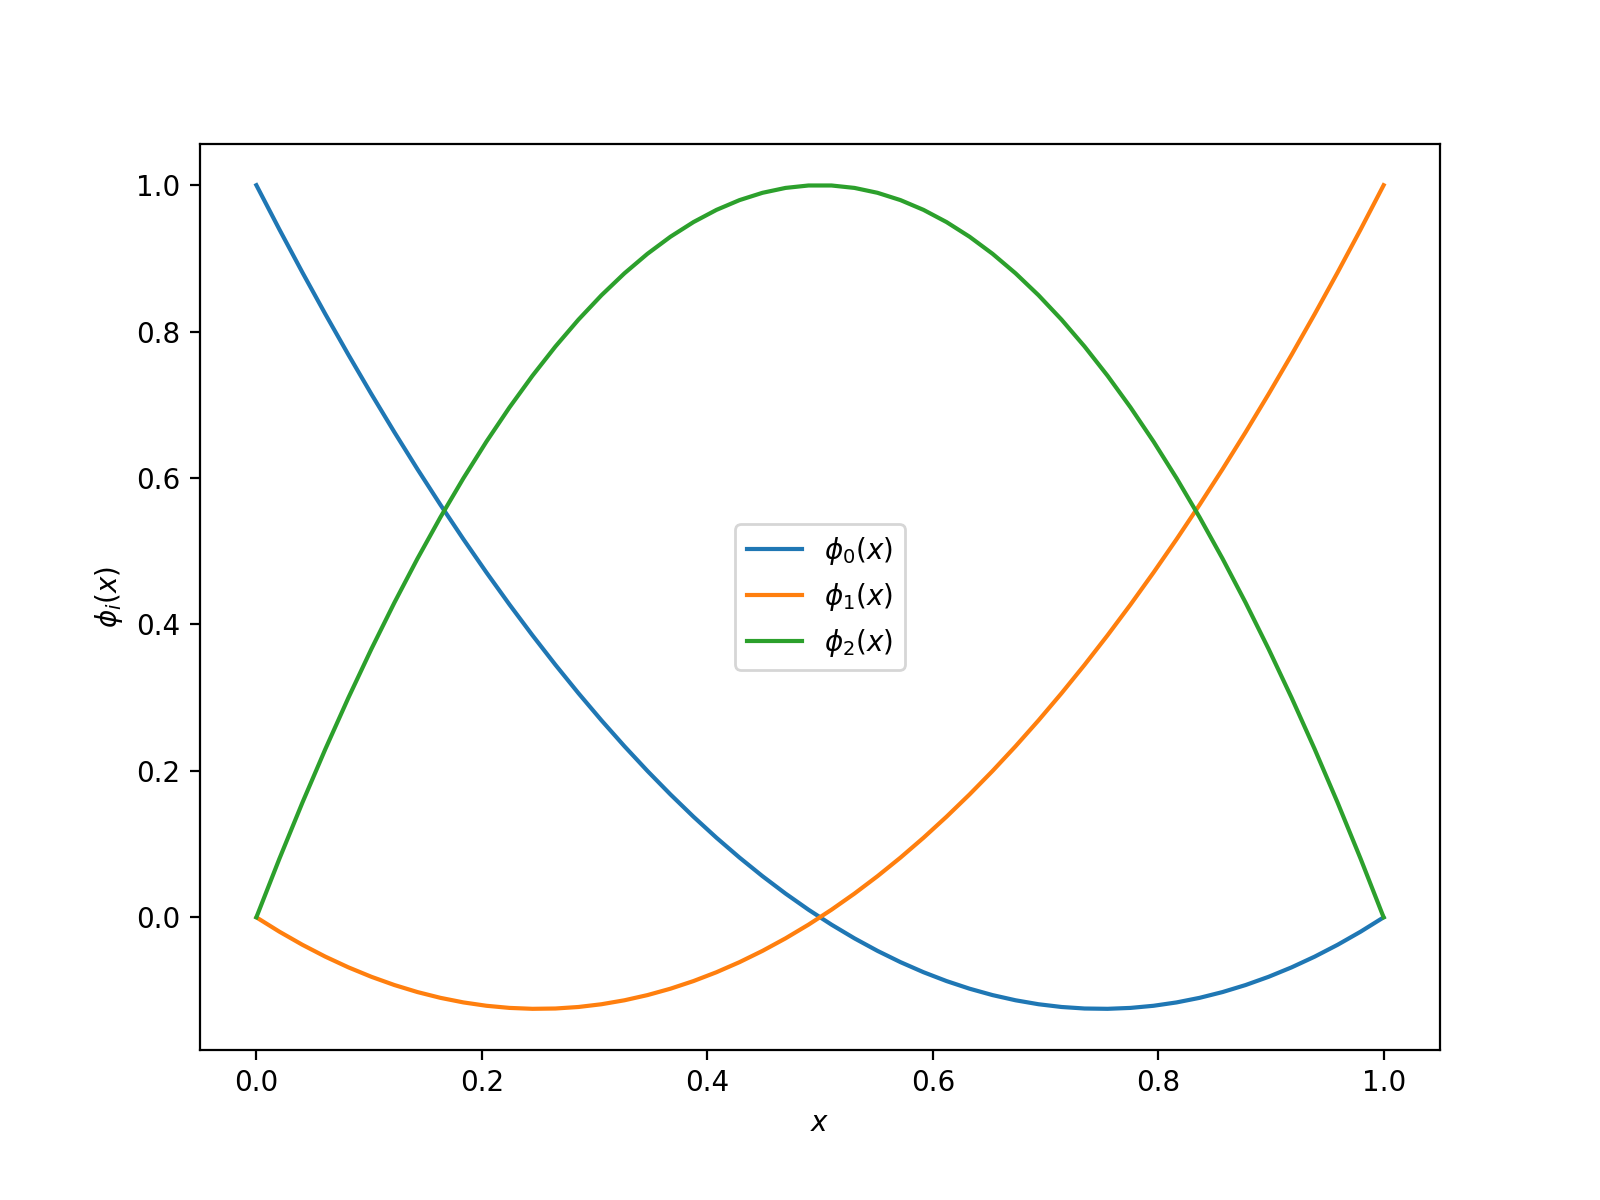
\includegraphics[width=\textwidth]{Pics/BasisFunc/IntervalFuncs.png}
     \caption{Lagrage order 2 basis functions  on interval $[0,1]$}
     \label{InterFuncs}
\end{figure}

\subsection{Triangle (2D)}
For a Lagrange element of order $2$ on a triangle we have $i \in \{0, 1, 2,3,4,5\}$ and the basis functions are of the form
\begin{equation}
\phi_i(x,y) = \xi_{i0} + \xi_{i1} x + \xi_{i2} y + \xi_{i3} xy + \xi_{i4} x^2 + \xi_{i5}y^2,
\end{equation}
where the domain is $x+y\leq 1, x \geq 0$ and $y\geq 0$. For $\ell_i$ we get
\begin{align}
\ell_0 &= (0,0), &\ell_3 = (1/2,1/2), \\
\ell_1 &= (1,0), &\ell_4 = (0,1/2), \\
\ell_2 &= (0,1), &\ell_5 = (1/2,0).
\end{align}
This leads to the set of equations
\begin{figure}[H]
 \begin{subfigure}{0.4\textwidth}
 \begin{align}
\phi_i(\ell_0) &= \xi_{i0}, \\
\phi_i(\ell_1) &= \xi_{i0} + \xi_{i1} + \xi_{i4}, \\
\phi_i(\ell_2) &= \xi_{i0} + \xi_{i2} + \xi_{i5},
 \end{align}
 \end{subfigure}
 \hfill
 \begin{subfigure}{0.6\textwidth}
 \begin{align}
 \phi_i(\ell_3) &= \xi_{i0} + \frac{\xi_{i1}+\xi_{i2}}{2} + \frac{\xi_{i3} + \xi_{i4} + \xi_{i5}}{4}, \\
 \phi_i(\ell_4) &= \xi_{i0} + \frac{\xi_{i2}}{2} + \frac{\xi_{i5}}{4},\\
 \phi_i(\ell_5) &= \xi_{i0} + \frac{\xi_{i1}}{2} + \frac{\xi_{i4}}{4}.
 \end{align}
 \end{subfigure}
 \hfill
\end{figure}
Therefore, using the equations created by (\ref{CG_eq}) we get the matrix of coefficients
\begin{align}
\left[ \begin{matrix}
\xi_{00} & \xi_{01} & \xi_{02} & \xi_{03} & \xi_{04} & \xi_{05}\\
\xi_{10} & \xi_{11} & \xi_{12} & \xi_{13} & \xi_{14} & \xi_{25}\\
\xi_{20} & \xi_{21} & \xi_{22} & \xi_{23} & \xi_{24} & \xi_{25}\\
\xi_{30} & \xi_{31} & \xi_{32} & \xi_{33} & \xi_{34} & \xi_{35}\\
\xi_{40} & \xi_{41} & \xi_{42} & \xi_{43} & \xi_{44} & \xi_{45}\\
\xi_{50} & \xi_{51} & \xi_{52} & \xi_{53} & \xi_{54} & \xi_{55}
\end{matrix} \right] &= 
\left[ \begin{matrix}
1 & 1 & 1 & 1 & 1 & 1\\
0 & 1 & 0 & 1/2 & 0 & 1/2\\
0 & 0 & 1 & 1/2 & 1/2 & 0\\
0 & 0 & 0 & 1/4 & 0 & 0\\
0 & 1 & 0 & 1/4 & 0 & 1/4\\
0 & 0 & 1 & 1/4 & 1/4 & 0
\end{matrix} \right]^{-1}, \\
\left[ \begin{matrix}
\xi_{00} & \xi_{01} & \xi_{02} & \xi_{03} & \xi_{04} & \xi_{05}\\
\xi_{10} & \xi_{11} & \xi_{12} & \xi_{13} & \xi_{14} & \xi_{25}\\
\xi_{20} & \xi_{21} & \xi_{22} & \xi_{23} & \xi_{24} & \xi_{25}\\
\xi_{30} & \xi_{31} & \xi_{32} & \xi_{33} & \xi_{34} & \xi_{35}\\
\xi_{40} & \xi_{41} & \xi_{42} & \xi_{43} & \xi_{44} & \xi_{45}\\
\xi_{50} & \xi_{51} & \xi_{52} & \xi_{53} & \xi_{54} & \xi_{55}
\end{matrix} \right] &= 
\left[ \begin{matrix}
1 & -3 & -3 & 4 & 2 & 2\\
0 & -1 & 0 & 0 & 2 & 0\\
0 & 0 & -1 & 0 & 0 & 2\\
0 & 0 & 0 & 4 & 0 & 0\\
0 & 0 & 4 & -4 & 0 & -4\\
0 & 4 & 0 & -4 & -4 & 0
\end{matrix} \right].
\end{align}
Thus leading to basis functions
\begin{align}
\phi_0(x,y) &= 2(x+y)^2 - 3(x+y) + 1, \\
\phi_1(x,y) &= x(2x-1), \\
\phi_2(x,y) &= y(2y-1), \\
\phi_3(x,y) &= 4xy, \\
\phi_4(x,y) &= 4y(1-x-y), \\
\phi_5(x,y) &= 4x(1-x-y).
\end{align}
With the visual representation in Figure \ref{triBasisFuncs}.
\begin{figure}[H]
 \begin{subfigure}{0.5\textwidth}
     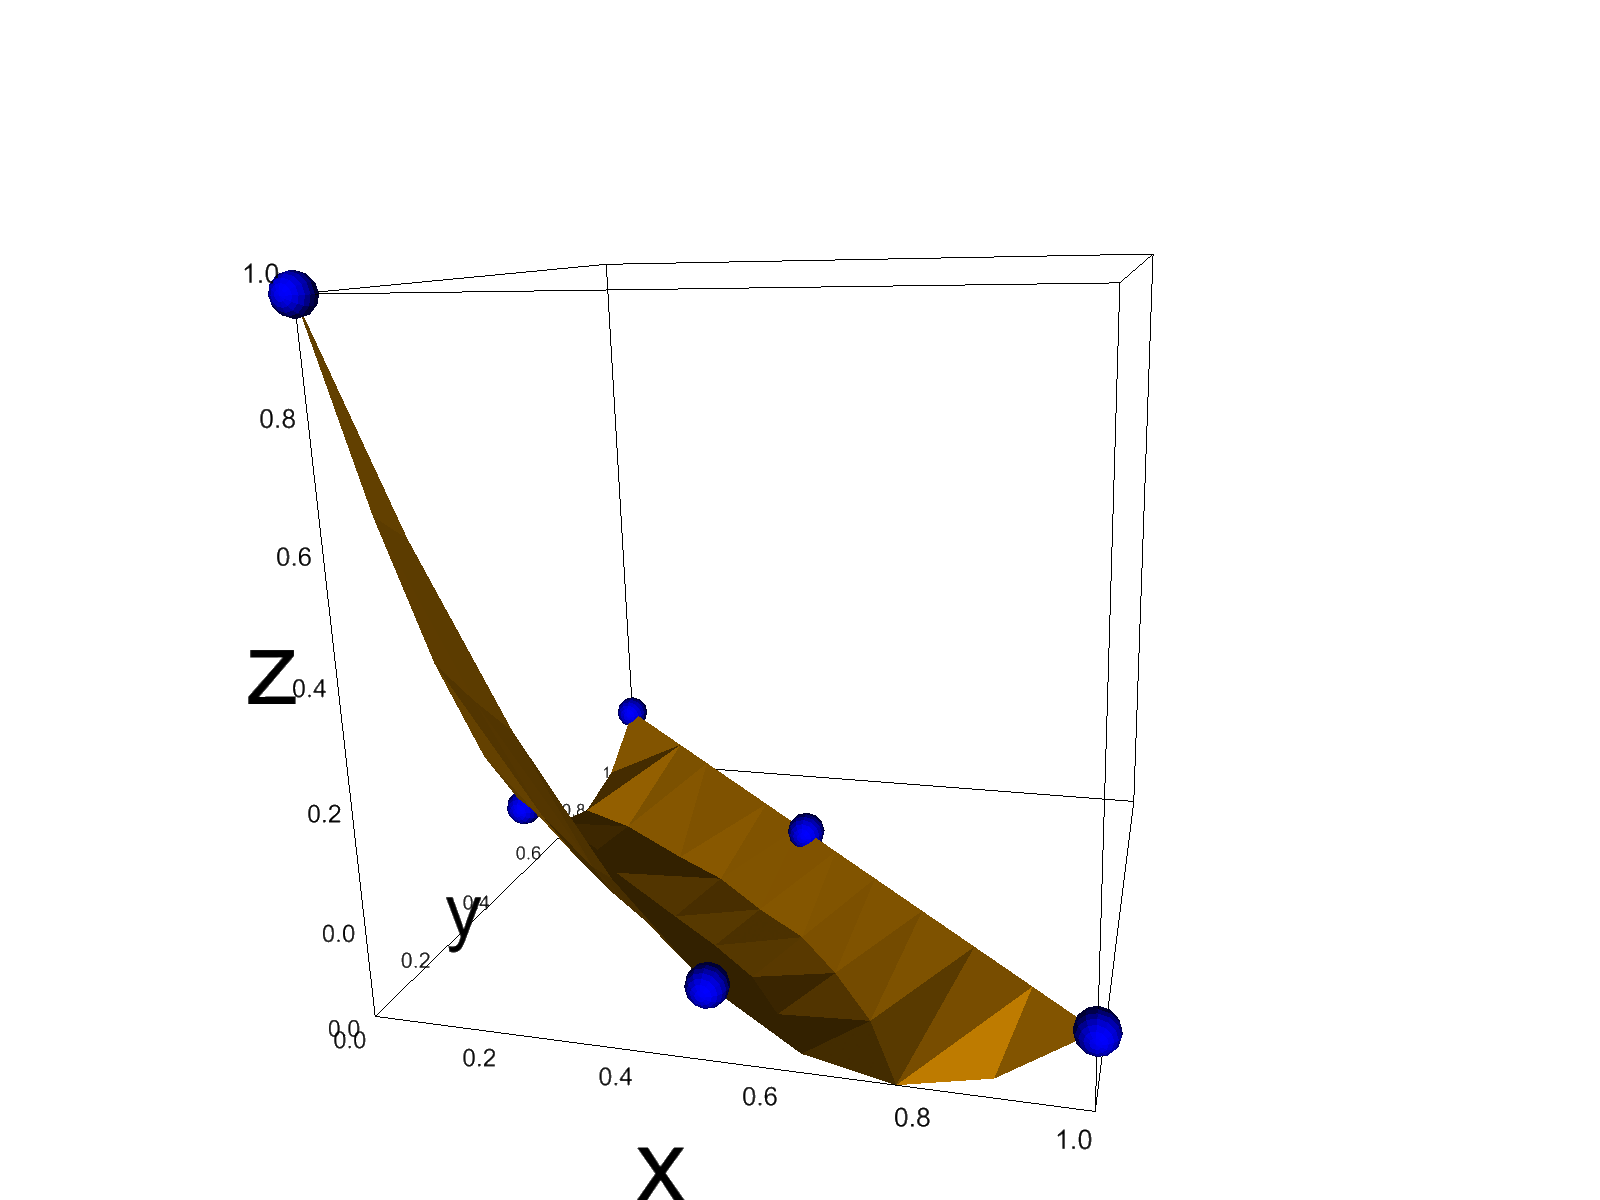
\includegraphics[width=\textwidth]{Pics/BasisFunc/triBasis0.png}
     \caption{$\phi_0(x,y) = 2(x+y)^2 - 3(x+y) + 1$,}
 \end{subfigure}
 \hfill
 \begin{subfigure}{0.5\textwidth}
     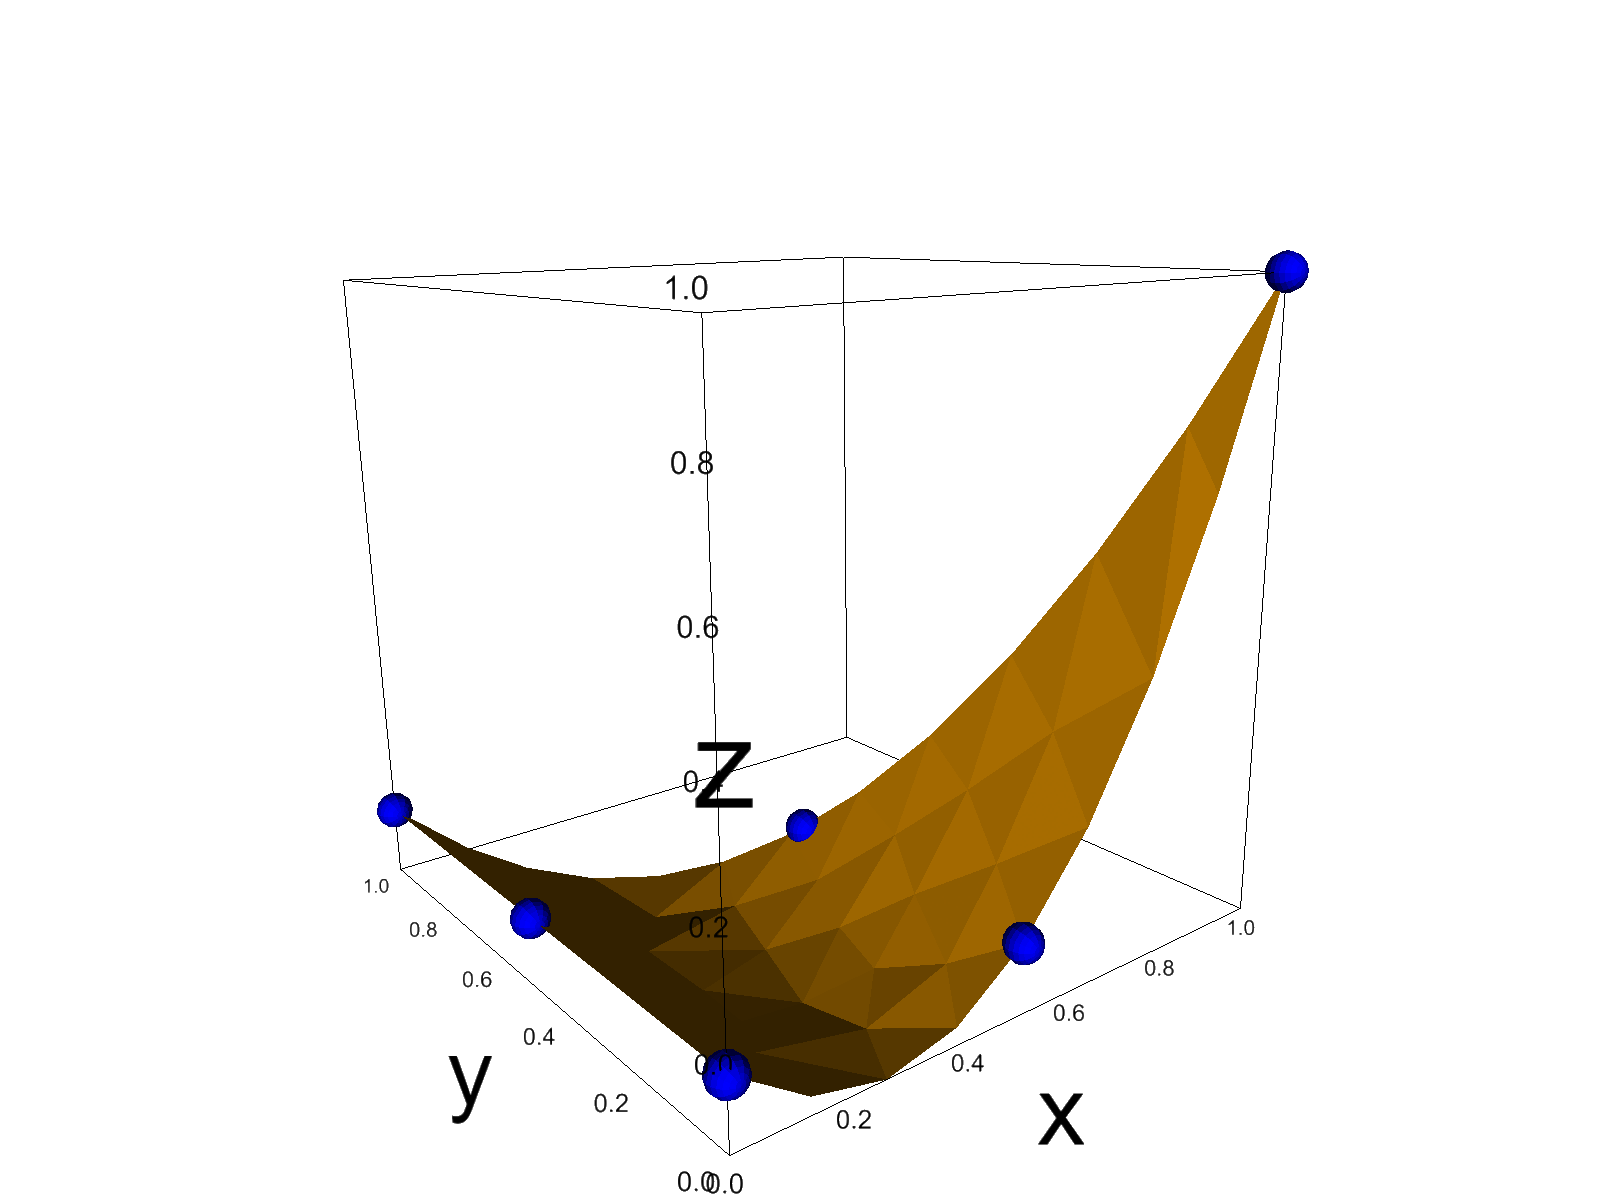
\includegraphics[width=\textwidth]{Pics/BasisFunc/triBasis1.png}
     \caption{$\phi_1(x,y) = x(2x-1)$,}
 \end{subfigure}
 \hfill
 \begin{subfigure}{0.5\textwidth}
     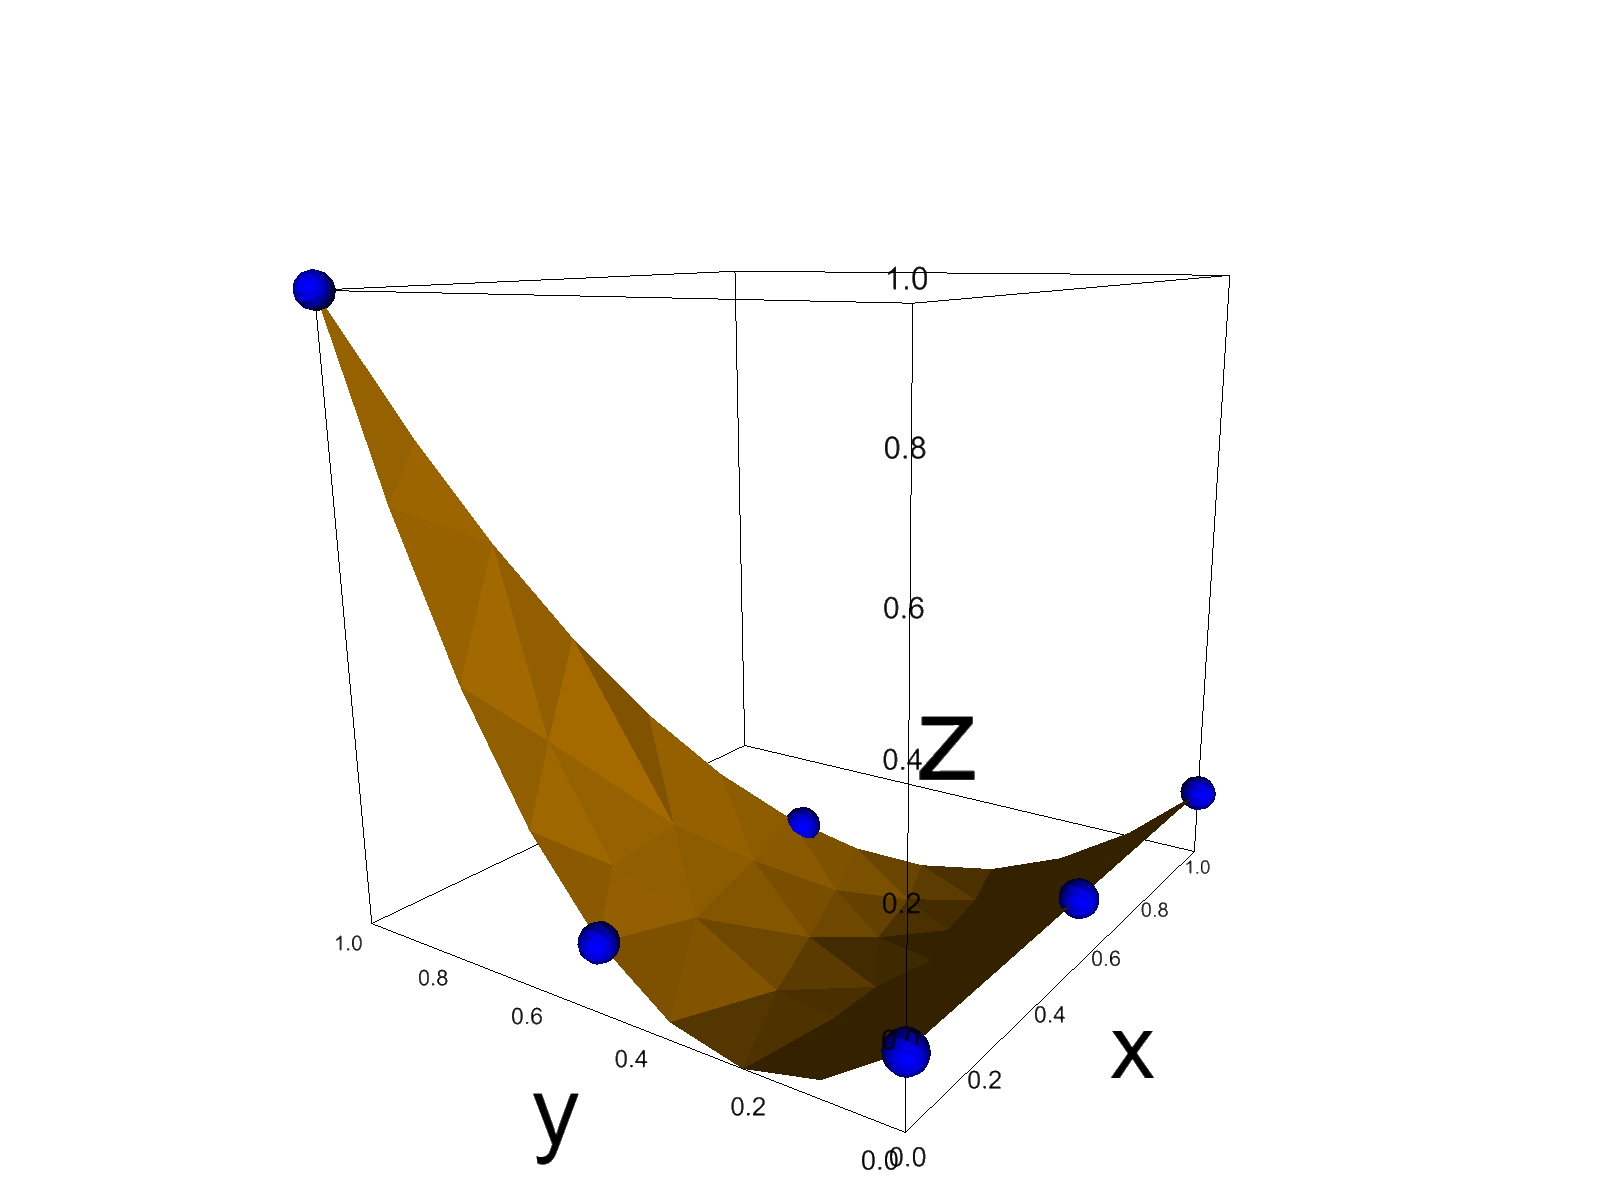
\includegraphics[width=\textwidth]{Pics/BasisFunc/triBasis2.png}
     \caption{$\phi_2(x,y) = y(2y-1)$,}
 \end{subfigure}
 \hfill
 \begin{subfigure}{0.5\textwidth}
     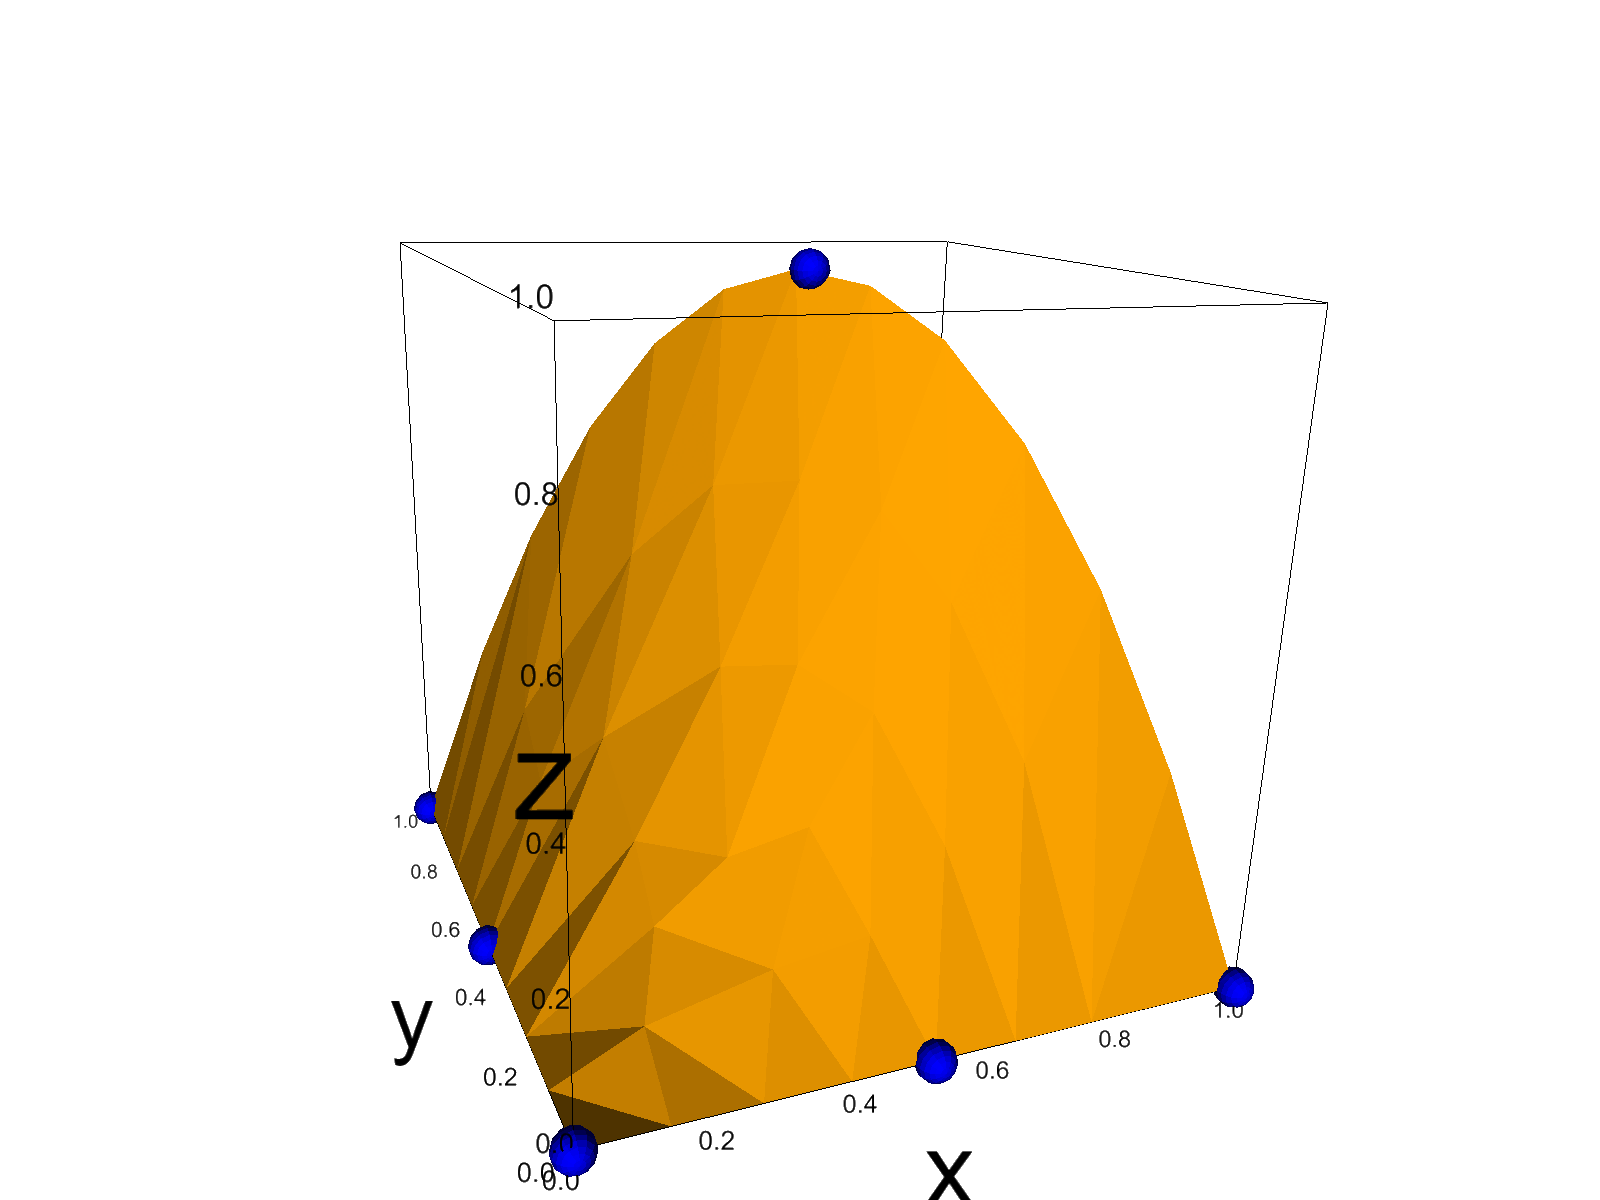
\includegraphics[width=\textwidth]{Pics/BasisFunc/triBasis3.png}
     \caption{$\phi_3(x,y) = 4xy$,}
 \end{subfigure}
 \hfill
 \begin{subfigure}{0.5\textwidth}
     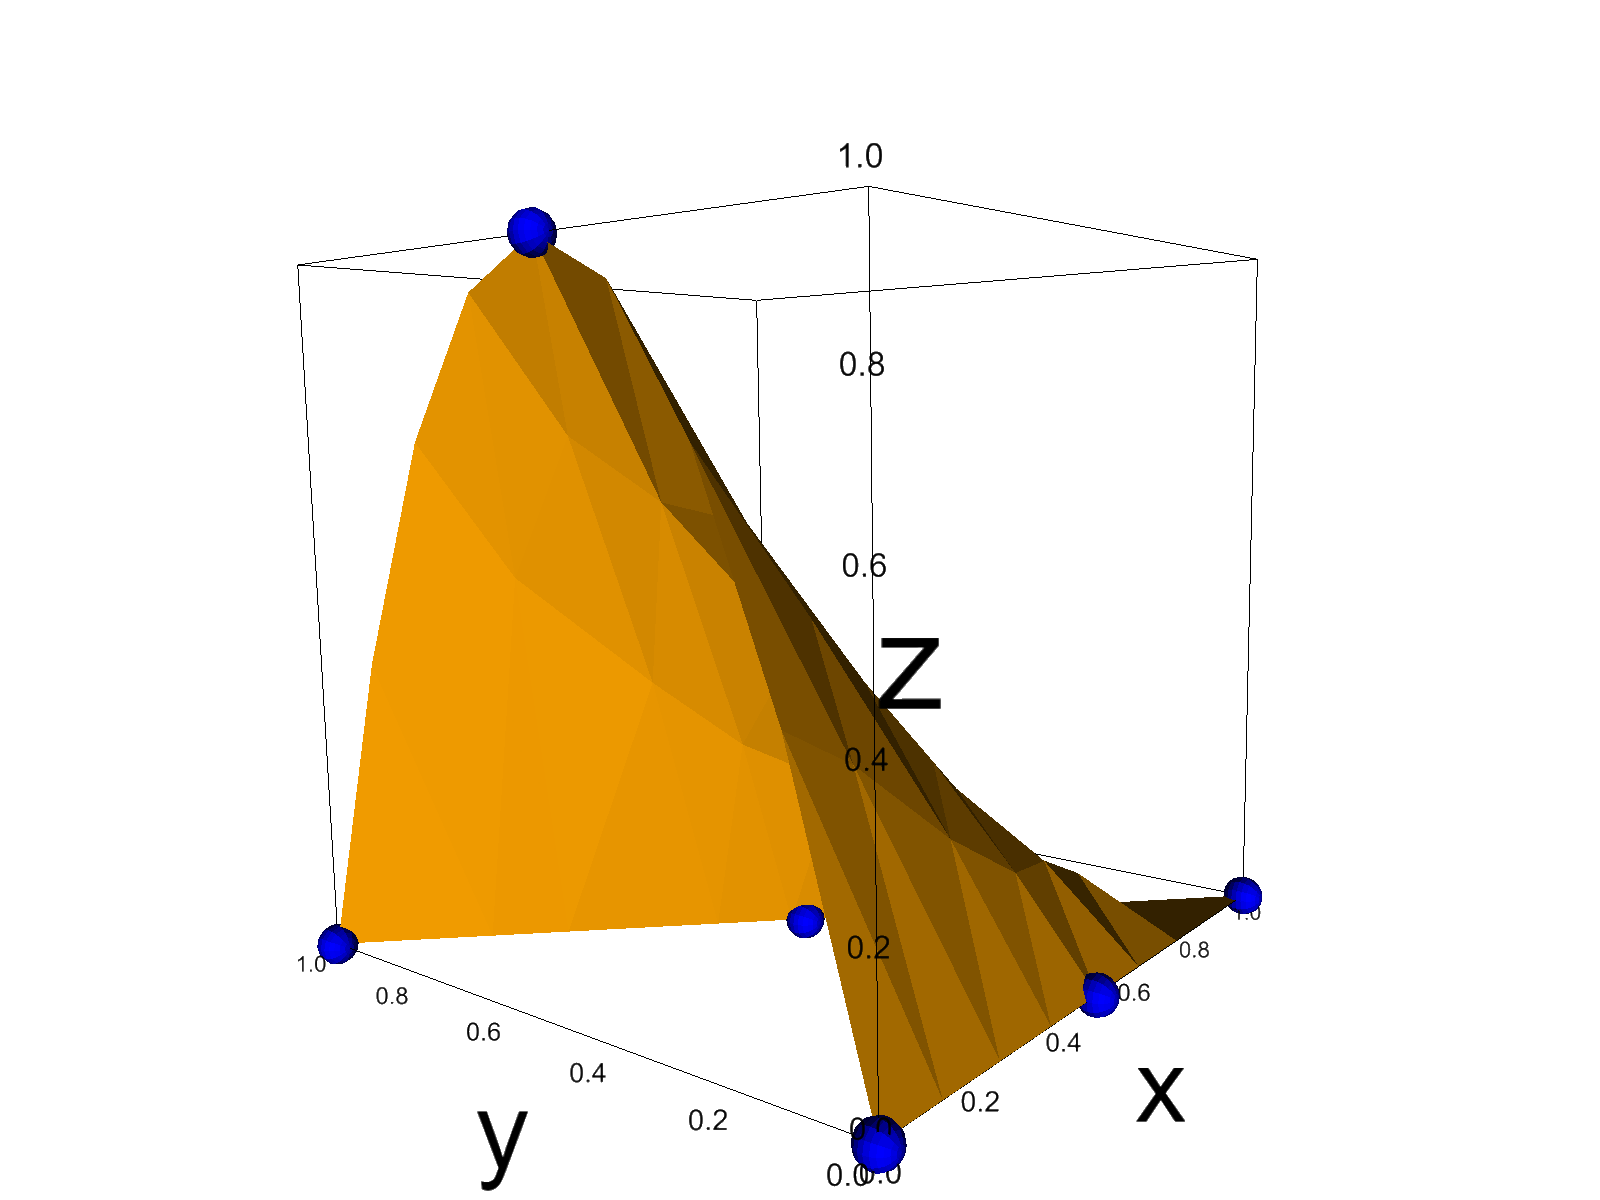
\includegraphics[width=\textwidth]{Pics/BasisFunc/triBasis4.png}
     \caption{$\phi_4(x,y) = 4y(1-x-y)$,}
 \end{subfigure}
 \hfill
 \begin{subfigure}{0.5\textwidth}
     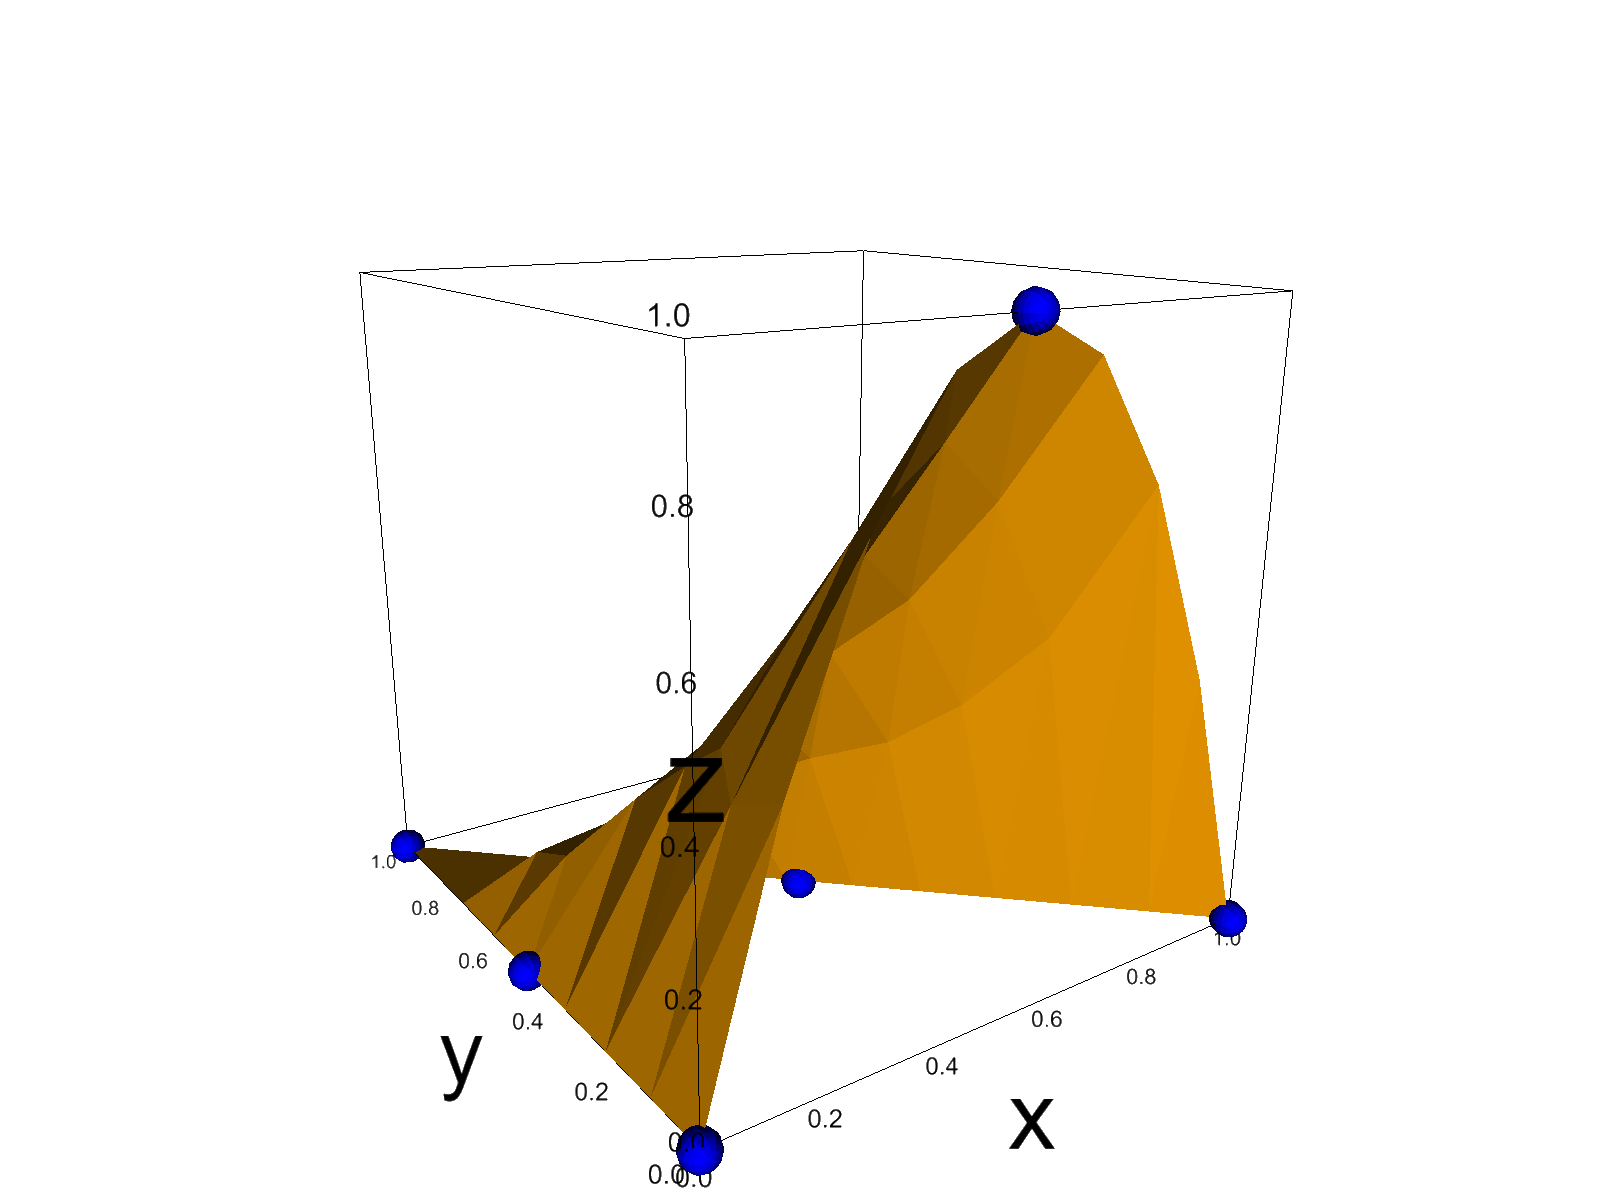
\includegraphics[width=\textwidth]{Pics/BasisFunc/triBasis5.png}
     \caption{$\phi_5(x,y) = 4x(1-x-y)$,}
 \end{subfigure}
 \hfill
 \caption{Basis Functions for Order 2 Lagrange Finite Element on a Triangle.} \label{triBasisFuncs}
\end{figure}

\section{Derivation of the Linear System}
We wish to find a matrix $\mathbb{B}^{(G)}$ and vector $\mathbf{F}^{(G)}$ so that the solution $\mathbf{u}$ to $\mathbb{B}^{(G)} \mathbf{u} = \mathbf{F}^{(G)}$ contains the coefficients for $u$ in the discretised space. We can use a local formulation approach on the domain of a single finite element $(\Omega_{FE})$. Thus we calculate the local $\mathbb{B}^{(L)}$ and $\mathbf{F}^{(L)}$. Then using a local to global map we add the results to the global system. Here is an algorithm to add the local system to the global system.
\lstinputlisting[language=Python]{CodeSnips/Global_Local_Map.py}
This approach is well known for one test function. But when multiple test functions are involved it may not be clear how this translates to a linear system. Thus we show the derivation of the linear system for the $(MMAP)$ method.

In these derivations of linear systems, we will use a finite element with two basis functions. In this case $d=2$. But it is trivial how to introduce more basis functions. Additionally, Firedrake \cite{Dragon} does this automatically thus it does not need to be implemented in code.
\subsection{Linear System for $(SP)$}
We will discrtise $u$ from (\ref{SP_w}) on the finite element domain with basis functions $\phi_0$ and $\phi_1$. Thus we substitute $u=u_0\phi_0 + u_1 \phi_1$ into (\ref{SP_w}) to get equations 
\begin{equation} \label{SP_Eqs}
\varepsilon^{-1}u_0a_{||}(\psi_0, \psi_i) +
\varepsilon^{-1}u_1a_{||}(\psi_1, \psi_i) +
u_0a_{\perp}(\psi_0, \psi_i) +
u_1a_{\perp}(\psi_1, \psi_i) =
\int_{\Omega_{FE}} f \psi_i d\mathbf{x}.
\end{equation}
For $i \in \{0,1\}$. It should be noted that the integrals are over the finite element domain $\Omega_{FE}$. Thus from (\ref{SP_Eqs}) we get linear system
\begin{equation} 
\left[
\begin{matrix}
\varepsilon^{-1}a_{||}(\psi_0, \psi_0) + a_{\perp}(\psi_0,\psi_0) &
\varepsilon^{-1}a_{||}(\psi_1, \psi_0) + a_{\perp}(\psi_1,\psi_0)\\
\varepsilon^{-1}a_{||}(\psi_0, \psi_1) + a_{\perp}(\psi_0,\psi_1) &
\varepsilon^{-1}a_{||}(\psi_1, \psi_1) + a_{\perp}(\psi_1,\psi_1)\\
\end{matrix}
\right] 
\left [
\begin{matrix}
u_0 \\
u_1
\end{matrix}
\right ] =
\left[
\begin{matrix}
\int_{\Omega_{FE}} f \psi_0 d\mathbf{x} \\
\int_{\Omega_{FE}} f \psi_1 d\mathbf{x}
\end{matrix}
\right].
\end{equation}
Then we add this local system to the global system. For $\varepsilon \ll 0$ we can see this matrix is ill-conditioned thus the $(SP)$ method only works for $\varepsilon \approx 1$.

\subsection{Linear System for $(MMAP)$}
Now we will discretise $u$ and  $q$ from (\ref{MMAP_w}). For the local formulation we get test functions $\hat{u}_0, \hat{u}_1, \hat{q_0}$ and $\hat{q_1}$. Now we substitute $u = u_0 \hat{u}_0 + u_1\hat{u}_1$ and $q = q_0\hat{q}_0 + q_1\hat{q}_1$ into (\ref{MMAP_w}). Thus we get equations
\begin{equation} \label{MMAP_Eqs}
\begin{cases}
u_0a_{\perp}(\hat{u}_0, \hat{u}_i) +
u_1a_{\perp}(\hat{u}_1, \hat{u}_i) +
q_0a_{||}(\hat{q}_0, \hat{u}_i) +
q_1a_{||}(\hat{q}_1, \hat{u}_i) &=
\int_{\Omega_{FE}} f \hat{u}_i d\mathbf{x}, \\
u_0a_{||}(\hat{u}_0, \hat{q}_i) +
u_1a_{||}(\hat{u}_1, \hat{q}_i) -
\varepsilon q_0a_{||}(\hat{q}_0, \hat{q}_i) -
\varepsilon q_1a_{||}(\hat{q}_1, \hat{q}_i) &=
0.
\end{cases}
\end{equation}
For $i\in\{0,1\}$. Thus from (\ref{MMAP_Eqs}), we get the linear system
\begin{equation}
\left [
\begin{matrix}
a_{\perp}(\hat{u}_0, \hat{u}_0) &
a_{\perp}(\hat{u}_1, \hat{u}_0) &
a_{||}(\hat{q}_0, \hat{u}_0) &
a_{||}(\hat{q}_1, \hat{u}_0) \\
a_{\perp}(\hat{u}_0, \hat{u}_1) &
a_{\perp}(\hat{u}_1, \hat{u}_1) &
a_{||}(\hat{q}_0, \hat{u}_1) &
a_{||}(\hat{q}_1, \hat{u}_1) \\
a_{||}(\hat{u}_0, \hat{q}_0) &
a_{||}(\hat{u}_1, \hat{q}_0) &
-\varepsilon a_{||}(\hat{q}_0, \hat{q}_0) &
-\varepsilon a_{||}(\hat{q}_1, \hat{q}_0) \\
a_{||}(\hat{u}_0, \hat{q}_1) &
a_{||}(\hat{u}_1, \hat{q}_1) &
-\varepsilon a_{||}(\hat{q}_0, \hat{q}_1) &
-\varepsilon a_{||}(\hat{q}_1, \hat{q}_1) \\
\end{matrix}
\right ]
\left [
\begin{matrix}
u_0 \\
u_1 \\
q_0 \\
q_1
\end{matrix}
\right ] =
\left [
\begin{matrix}
\int_{\Omega_{FE}}f\hat{u}_0 d \mathbf{x} \\
\int_{\Omega_{FE}}f\hat{u}_1 d \mathbf{x} \\
0 \\
0
\end{matrix}
\right ].
\end{equation}
Then we add this local system to the global system. We can see this matrix is well-conditioned thus the $(MMAP)$ method works for $0<\varepsilon<1$.

\section{Example 1}
We will solve the PDE (\ref{PDE}) with $\Omega = [0,1]^2, \Gamma_D = \{y=0 \text{ or } y=1\}$ and $\Gamma_N = \{x=0 \text{ or } x=1\}$. We chose a magnetic field such
\begin{equation} \label{E1_b}
\mathbf{b} = \frac{\mathbf{B}}{|\mathbf{B}|}, 
\mathbf{B} = \left[ \begin{matrix}
\alpha(2y-1)\cos(m\pi x) + \pi\\
\alpha m \pi (y^2-y)\sin(m \pi x)
\end{matrix} \right]
\end{equation}
Thus we have $\Gamma_{in}:= \{x=0\}$ and we have the streamlines defined by 
\begin{equation}
\pi y + \alpha (y^2-y) \cos(m\pi x) = C,
\end{equation}
with $0 \leq C \leq \pi$. This is calculated in Appendix \ref{E1_Stream_Calc}. We have the solution must be constant along streamlines for $\varepsilon \ll 1$. We calculate the streamlines to find exact solutions to test. This leads to an exact solution 
\begin{equation} \label{E1_u}
u = \sin(\pi y + \alpha (y^2-y) \cos(m\pi x)) + \varepsilon \cos(2 \pi x) \sin(\pi y)
\end{equation}
This test problem came from \cite{DN}. However, the same or similar problem is very popular and appears in papers \cite{LINE_INT}, \cite{AP}, \cite{MMAP} and \cite{STAB}. We will cover three sub-examples with $(\alpha=0),(\alpha=2,m=1)$ and $(\alpha = 2, m=10)$. Thus we get electromagnetic fields shown in Figure \ref{E1_VFs}. The field for $\alpha = 0$ is not shown as it is a simple vector field with $\mathbf{b}= [1, 0]$.
\begin{figure}[H]
 \begin{subfigure}{0.5\textwidth}
     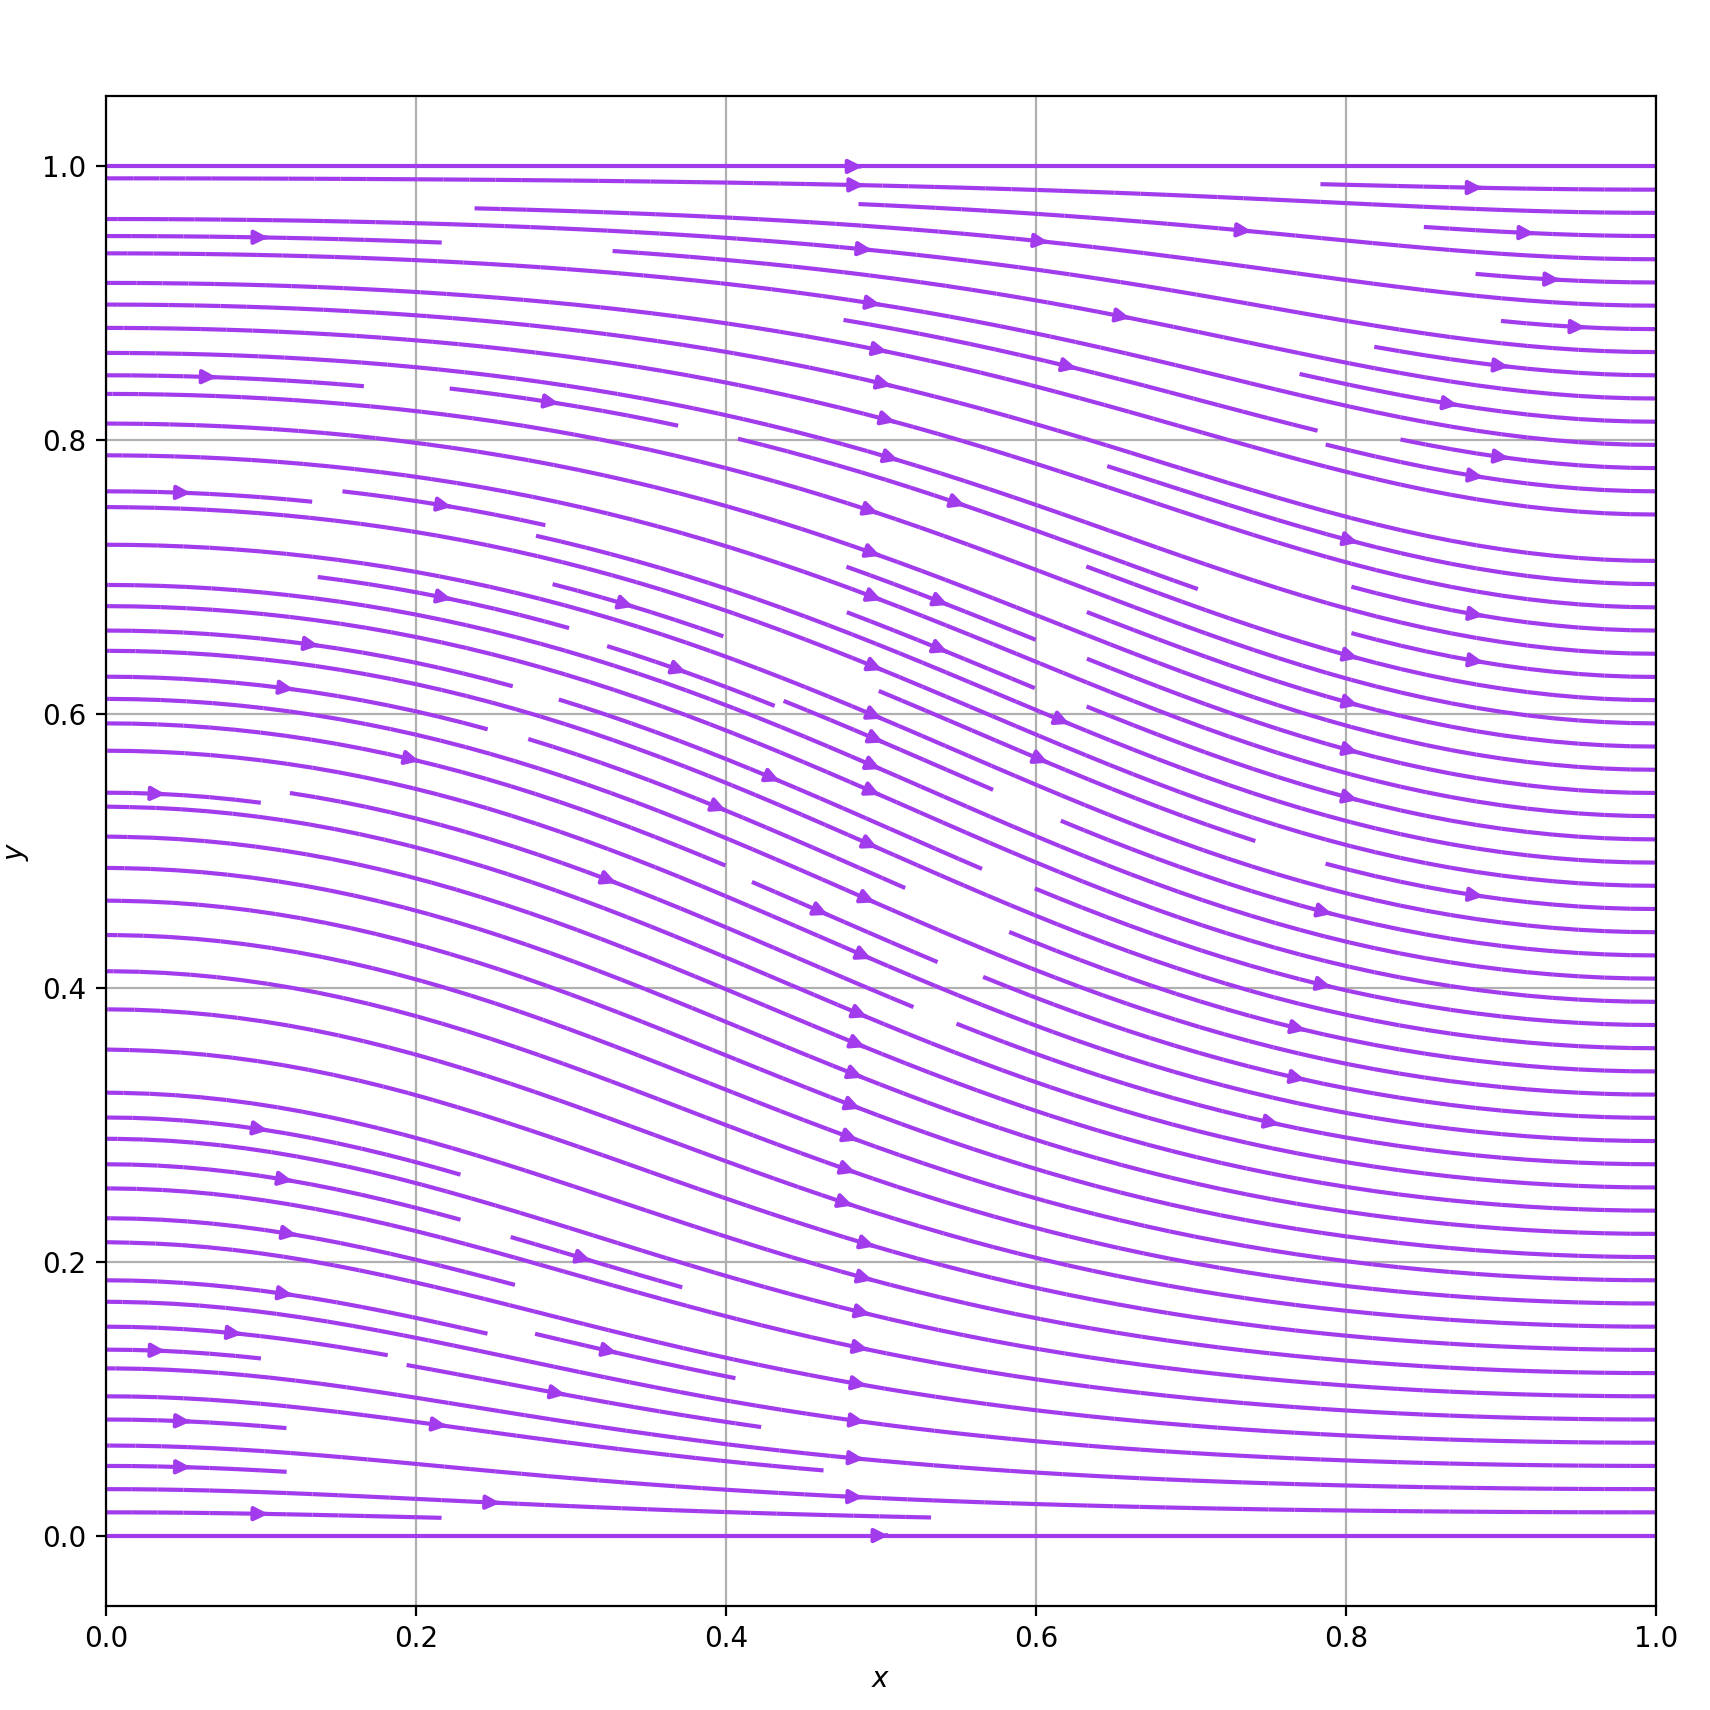
\includegraphics[width=\textwidth]{Pics/VectorField/E1b_a2_m1.png}
     \caption{$\alpha=2, m=1$}
 \end{subfigure}
   \begin{subfigure}{0.5\textwidth}
     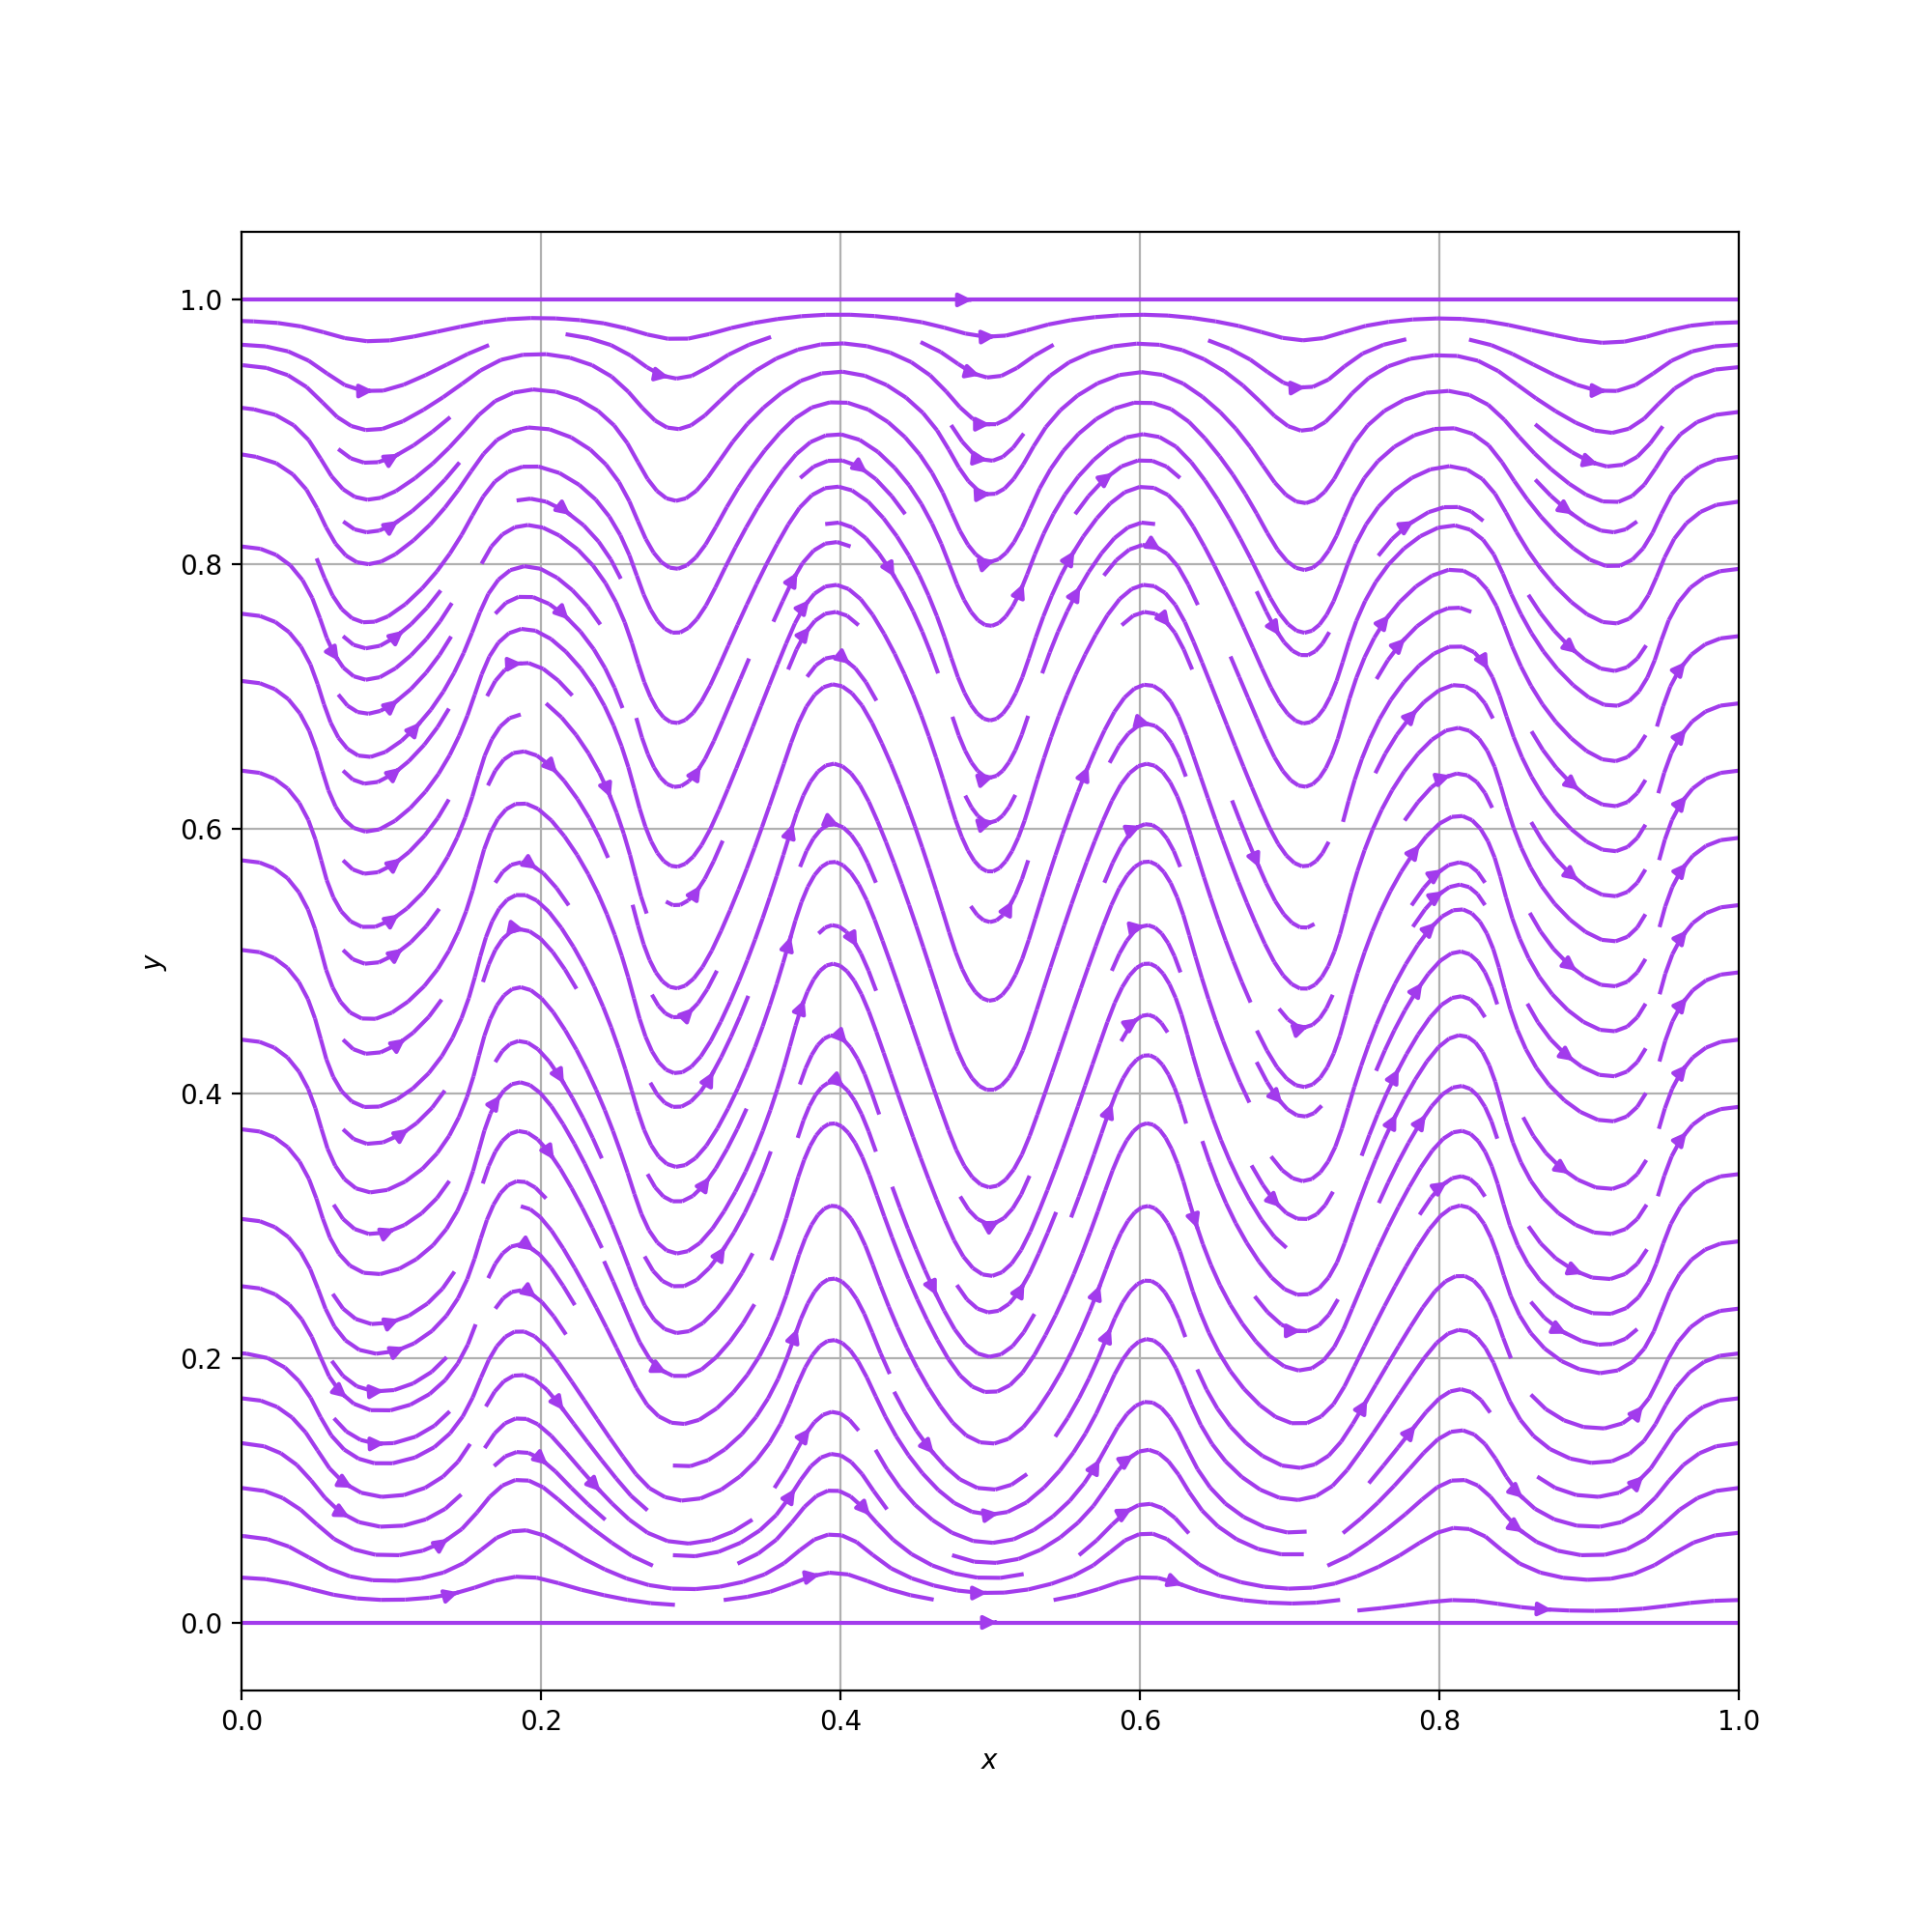
\includegraphics[width=\textwidth]{Pics/VectorField/E1b_a2_m10.png}
     \caption{$\alpha=2, m=10$}
 \end{subfigure}
 \caption{Electromagetic vector field $\mathbf{b}$ from (\ref{E1_b})} \label{E1_VFs}
\end{figure}
In Figure \ref{E1_us} we have the exact solution $u$ (\ref{E1_u}) to example $1$. We have the source term $f$ which is too complicated to write analytically so the visualisation is given in Figure \ref{E1_fs}. We analysis the equation with $\varepsilon = 0.1$ and $\varepsilon = 10^{-10}$. We notice the $\varepsilon = 0.1$ and $\varepsilon = 10^{-10}$ variants are visually similar for the source term $f$ and exact term $u$ this suggests we should consider a method discussed in section \ref{MAP_f}. The main difference is the solution $u$ is not constant on streamlines of the vector field $\mathbf{b}$ this makes logical sense because increasing the anisotropic strength (make $\varepsilon$ smaller) leads to less diffusion perpendicular to the magnetic field and undisturbed diffusion parallel to the magnetic field.

In Figures \ref{E1_LH_PF} and \ref{E1_LM_SP} we numerically simulate the PDE created by Example $1$ with a $20 \times 20$ grid, where each finite element is a square with width $0.05$ discretised with an order $2$ Lagrange element. Also, each red dot represents a numerical calculation with varying $\varepsilon$. Where the degrees of freedom for $(MMAP), (PF), (LM)$ are $3362$, $(SP)$ is $1681$ and $(AP)$ is $8405$.

In Figure \ref{E1_LH_PF} we compare methods $(MMAP), (PF)$ and $(AP)$. The error plot for $(MMAP)$ is located under the error plot for $(AP)$ this strongly suggests these methods will calculate a similar value for the error. Thus for further numerical calculations, we will only consider the $(MMAP)$ because for similar error it has fewer degrees of freedom than the $(AP)$ method. This decreases the amount of computational power used. Additionally, when the vector field is not anisotropic $(\alpha = 0)$ all methods produce small error for $0 <\varepsilon \leq 1$. Also, Figure \ref{E1_Mild_Ans} visually suggests when the vector field is mildly anisotropic the $(MMAP)$ method performs better than the $(PF)$ method. However, from Figure \ref{E1_Strong_Ans} we infer when the vector field is highly anisotropic $(PF)$ performs better than $(MMAP)$. 

In the numerical calculations shown in Figure \ref{E1_LM_SP}, it follows our logic that the $(LM)$ method produces a small error for $\varepsilon \ll 1$ and a much larger error for $\varepsilon \approx 1$. Also, it shows the $(SP)$ method failing when $\varepsilon \ll 1$. This strongly suggests that we have implemented our code correctly. For further numerical calculations we use $(MMAP)$ instead of $(LM)$ and $(SP)$ as in Figure \ref{E1_LM_SP} $(MMAP)$ has the smallest error for  $0 < \varepsilon \leq 1$.

However, the $(SP)$ method has fewer degrees of freedom than the $(MMAP)$ method and from Figure \ref{E1_LM_SP} there exists an $\varepsilon_0$ where when $\varepsilon \geq \varepsilon_0$ the $(SP)$ method has a similar error to the $(MMAP)$ method. Thus we can propose a new method that involves using $(MMAP)$ when $\varepsilon < \varepsilon_0$ and using the $(SP)$ method when $\varepsilon \leq \varepsilon_0$. One problem with this method is that when the PDE becomes more anisotropic $\varepsilon_0$ increases and we are interested in methods for solving highly anisotropic diffusion problems with $\varepsilon \ll 1$. Thus this method is not further discussed.

\begin{table}[H]
\resizebox{\textwidth}{!}{
\begin{tabular}{||cccccccc||}
\cline{3-8}
\multicolumn{2}{c|}{L2 Error} & \multicolumn{2}{c|}{$\alpha = 0$} & \multicolumn{2}{c|}{$\alpha = 2, m=1$} & \multicolumn{2}{c|}{$\alpha = 2, m=10$} \\
\hline 
Size          & dof          & PF        & MMAP        & PF        & MMAP        & PF        & MMAP        \\
\hline \hline
$10\times 10$  &  882    &  $1.26\times10^{-4}$ & $1.26\times10^{-4}$  & $1.64\times10^{-1}$ & $2.25\times10^{-4}$ & $4.29\times10^{-2}$ & $3.16\times10^{-1}$\\
\hline
$20\times 20$  &  3362     & $1.58\times 10^{-5}$ & $1.58\times 10^{-5}$ & $4.01\times10^{-2}$ & $2.80\times10^{-5}$ & $2.94\times10^{-2}$ & $1.25\times10^{-1}$\\
\hline
$40\times 40$ &   13122    & $1.97\times 10^{-6}$ & $1.97\times 10^{-6}$ & $1.42\times10^{-3}$ & $3.44\times10^{-6}$ & $4.23\times 10^{-3}$ & $1.29\times10^{-2}$\\
\hline
$80\times 80$  &  51842     & $2.46\times 10^{-7}$ & $2.46\times 10^{-7}$ & $2.38\times10^{-5}$ & $4.25 \times 10^{-7}$ & $9.71\times10^{-4}$ & $9.70\times10^{-4}$\\
\hline
$160\times 160$ & 206082   & $3.09\times 10^{-8}$ & $3.09\times 10^{-8}$ & $1.47\times10^{-6}$ & $5.25 \times 10^{-8}$ & $2.19\times10^{-4}$ & $6.36\times10^{-5}$ \\
\hline
\end{tabular}}
\end{table}


\begin{table}[H]
\resizebox{\textwidth}{!}{
\begin{tabular}{||cccccccc||}
\cline{3-8}
\multicolumn{2}{c|}{H1 Error} & \multicolumn{2}{c|}{$\alpha = 0$} & \multicolumn{2}{c|}{$\alpha = 2, m=1$} & \multicolumn{2}{c|}{$\alpha = 2, m=10$} \\
\hline 
Size          & dof          & PF        & MMAP        & PF        & MMAP        & PF        & MMAP        \\
\hline \hline
$10\times 10$  &  882    &  $8.16\times10^{-3}$ & $8.16\times10^{-3}$  & $1.00\times10^{0}$ & $1.42\times10^{-2}$ & $2.57\times10^{1}$ & $4.22\times10^{0}$\\
\hline
$20\times 20$  &  3362     & $2.04\times 10^{-3}$ & $2.04\times 10^{-3}$ & $3.99\times10^{-1}$ & $3.57\times10^{-3}$ & $1.21\times10^{1}$ & $1.99\times10^{0}$\\
\hline
$40\times 40$ &   13122    & $5.11\times 10^{-4}$ & $5.11\times 10^{-4}$ & $4.37\times10^{-2}$ & $8.89\times10^{-4}$ & $4.38\times 10^{-1}$ & $3.20\times10^{-1}$\\
\hline
$80\times 80$  &  51842     & $1.28\times 10^{-4}$ & $1.28\times 10^{-4}$ & $7.23\times10^{-3}$ & $2.21\times 10^{-4}$ & $2.01\times10^{-1}$ & $5.00\times10^{-2}$\\
\hline
$160\times 160$ & 206082   & $3.19\times 10^{-5}$ & $3.19\times 10^{-5}$ & $1.77\times10^{-3}$ & $5.49\times 10^{-5}$ & $9.79\times10^{-2}$ & $ 1.10\times10^{-2}$ \\
\hline
\end{tabular}}
\caption{Error for varying quadrilateral grid size for variants of Example $1$ using $(PF)$ and $(MMAP)$ with order $2$ Lagrange finite element and $\varepsilon=10^{-10}$.}
\label{tlb_E1_Error}
\end{table}

As can be seen in Table \ref{tlb_E1_Error} when the number of finite elements in the grid has increased the error is reduced.

\begin{figure}[H]
 \begin{subfigure}{0.5\textwidth}
     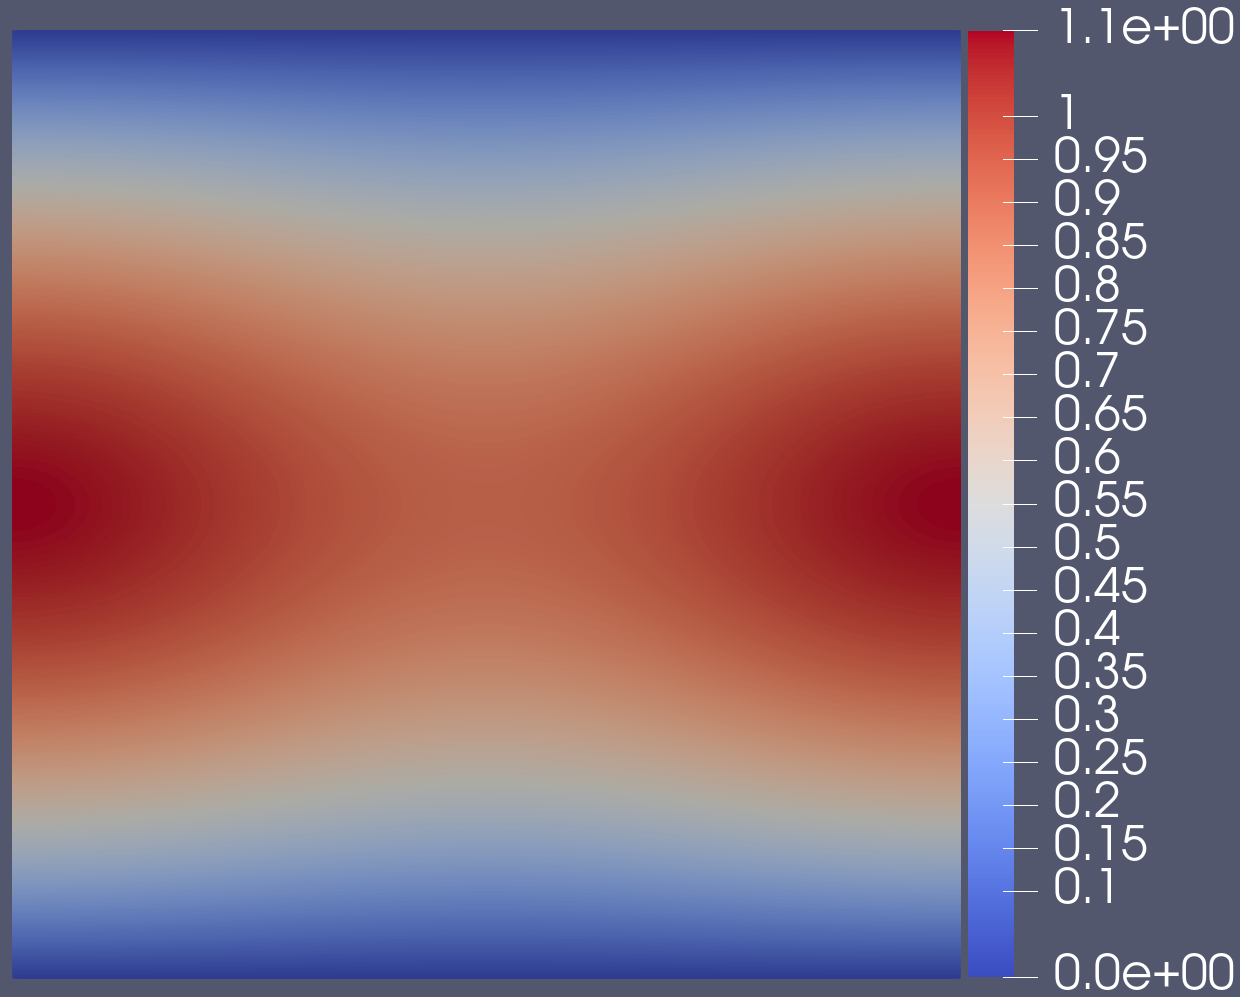
\includegraphics[width=\textwidth]{Pics/uf/U_E1a_eps1.png}
     \caption{$\alpha=0$ and $\varepsilon = 0.1$}
 \end{subfigure}
   \begin{subfigure}{0.5\textwidth}
     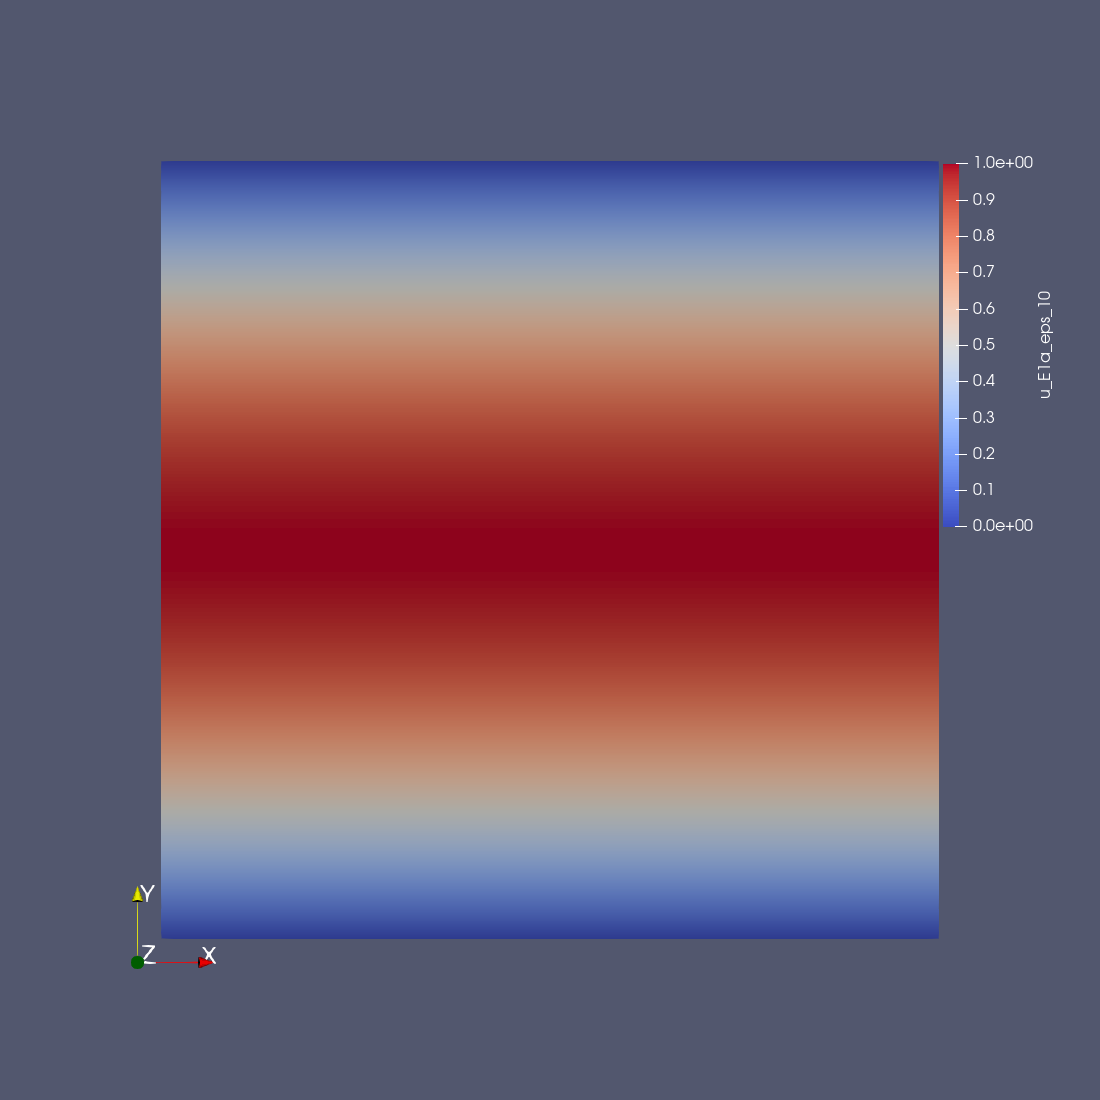
\includegraphics[width=\textwidth]{Pics/uf/U_E1a_eps10.png}
     \caption{$\alpha=0$ and $\varepsilon = 10^{-10}$}
 \end{subfigure}
 \begin{subfigure}{0.5\textwidth}
     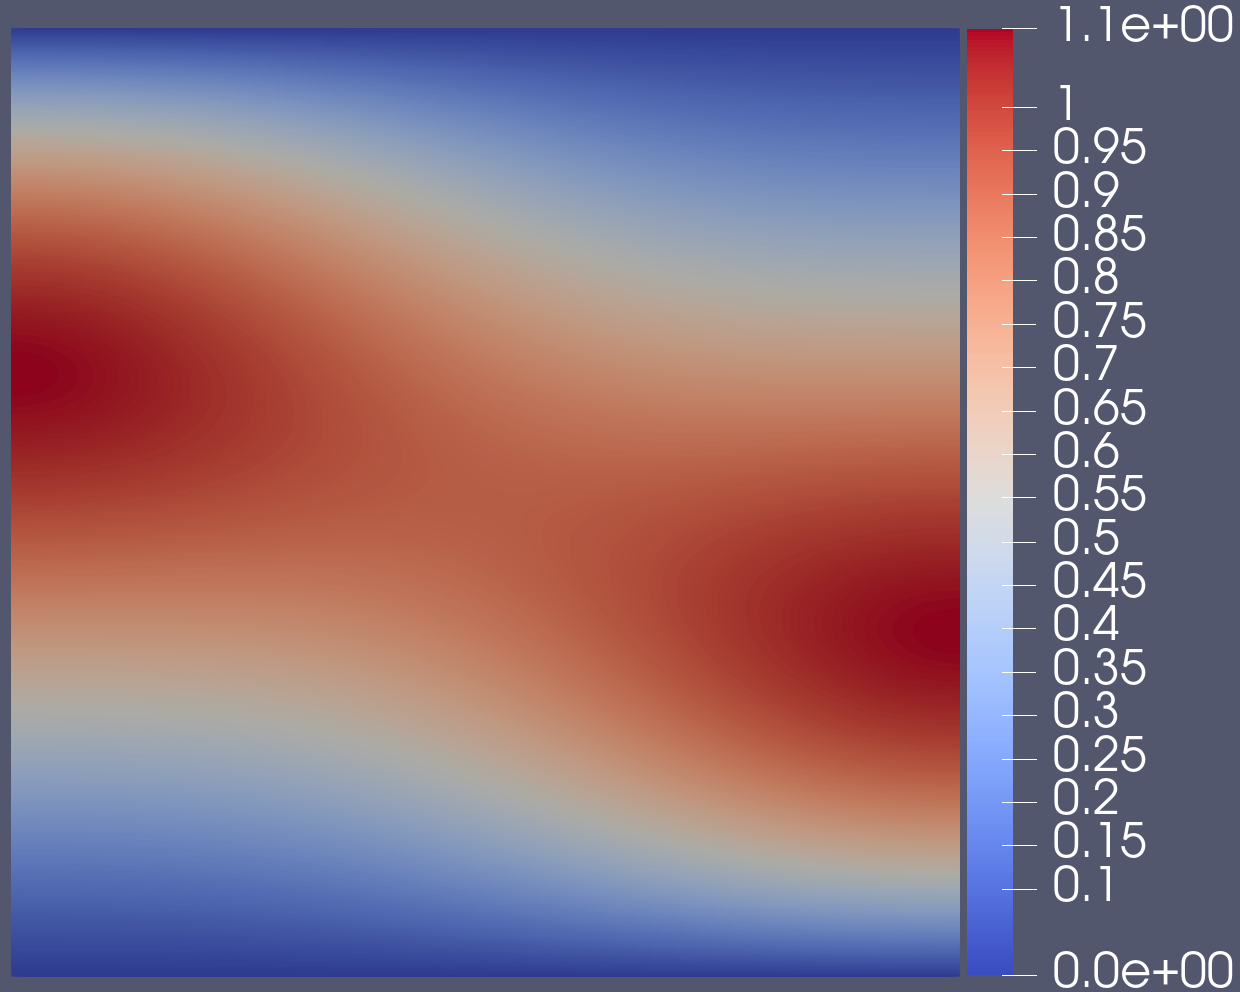
\includegraphics[width=\textwidth]{Pics/uf/U_E1b_eps1.png}
     \caption{$\alpha=2, m=1$ and $\varepsilon = 0.1$}
 \end{subfigure}
 \begin{subfigure}{0.5\textwidth}
     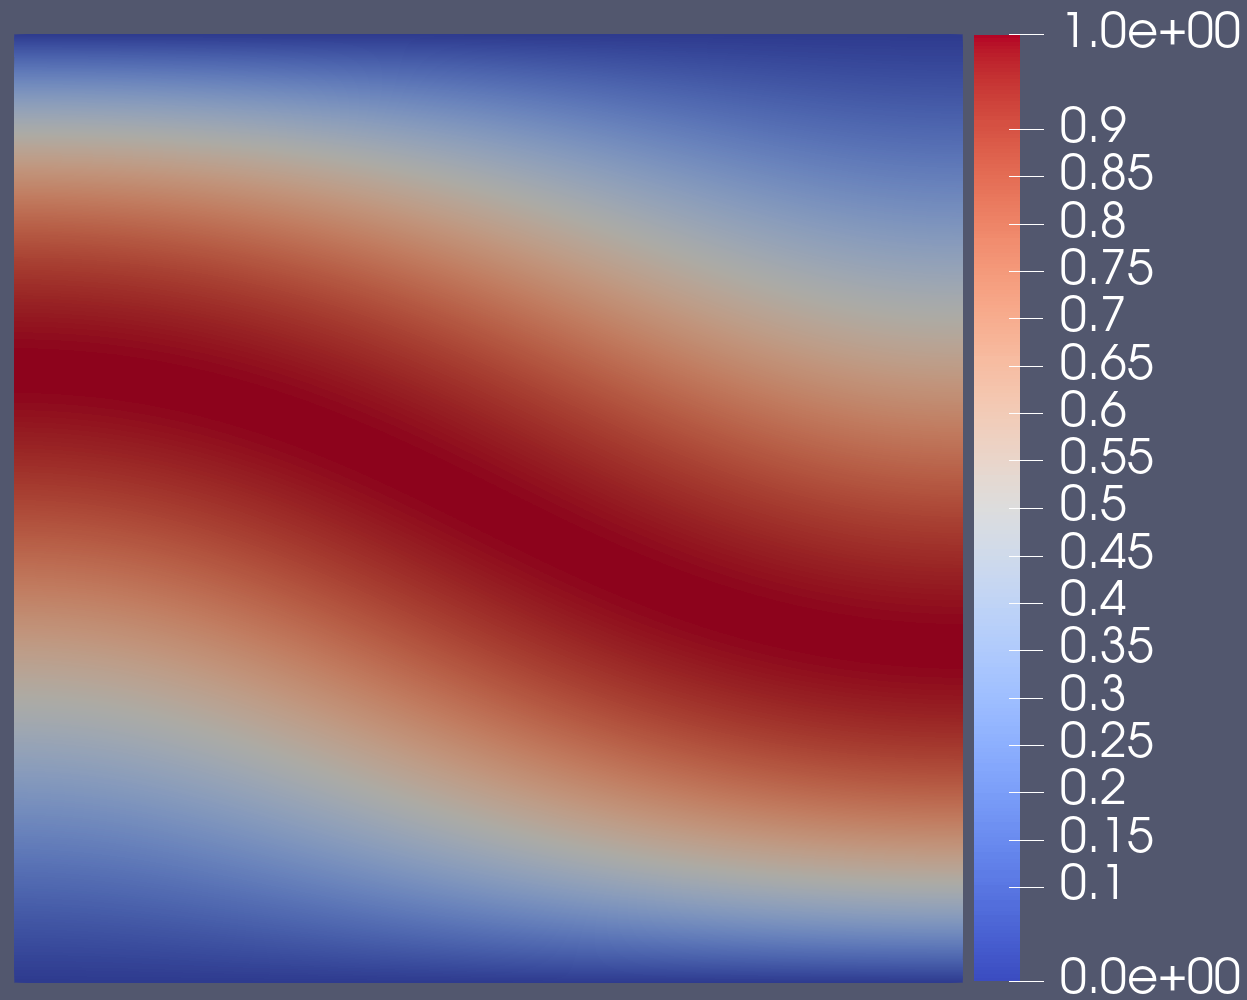
\includegraphics[width=\textwidth]{Pics/uf/U_E1b_eps_10.png}
     \caption{$\alpha=2, m=1$ and $\varepsilon = 10^{-10}$}
 \end{subfigure}
 \begin{subfigure}{0.5\textwidth}
     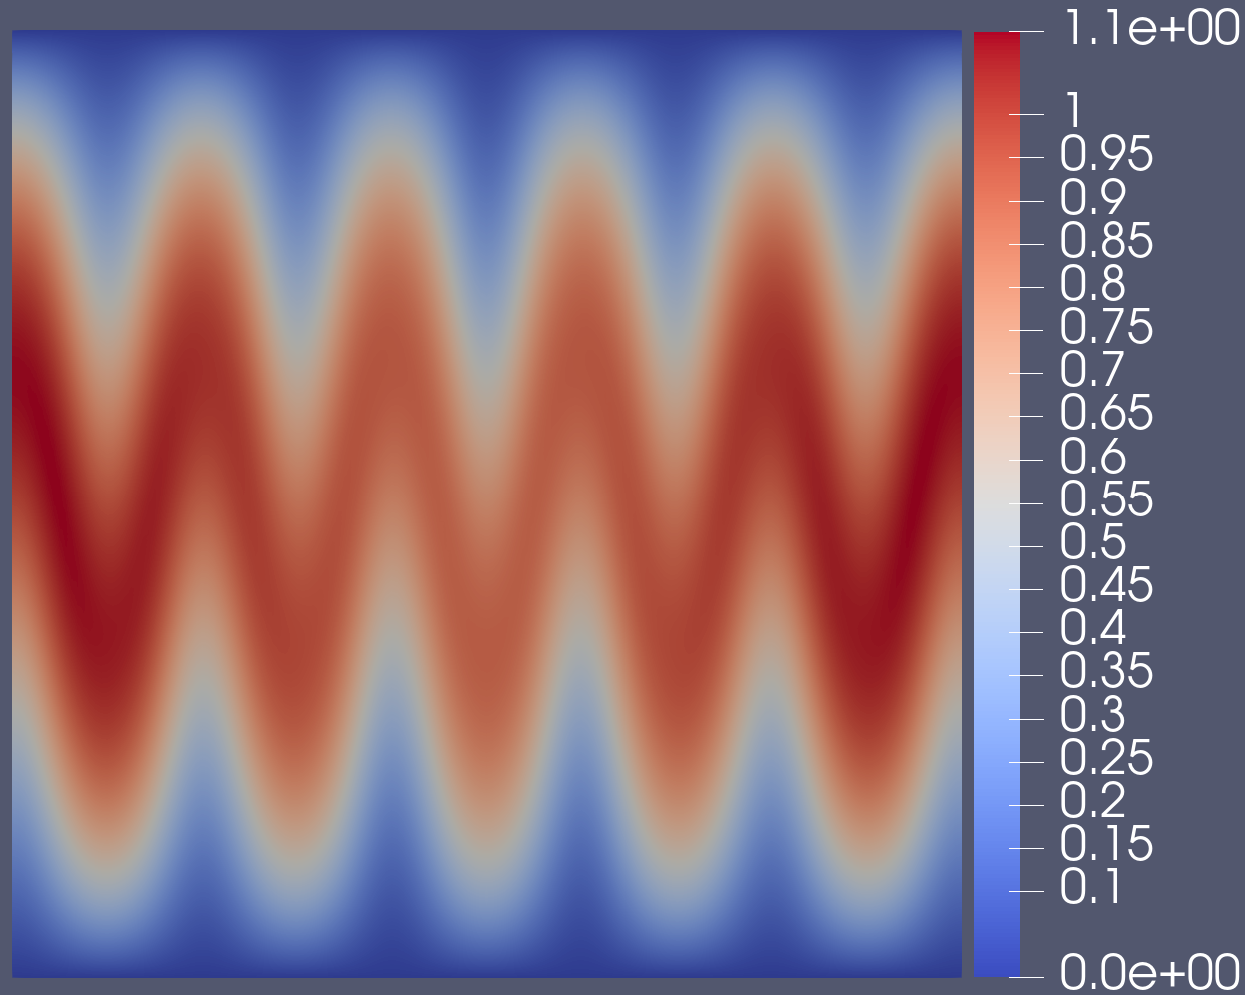
\includegraphics[width=\textwidth]{Pics/uf/U_E1c_eps_1.png}
     \caption{$\alpha=2, m=10$ and $\varepsilon = 0.1$}
 \end{subfigure}
 \hfill
 \begin{subfigure}{0.5\textwidth}
     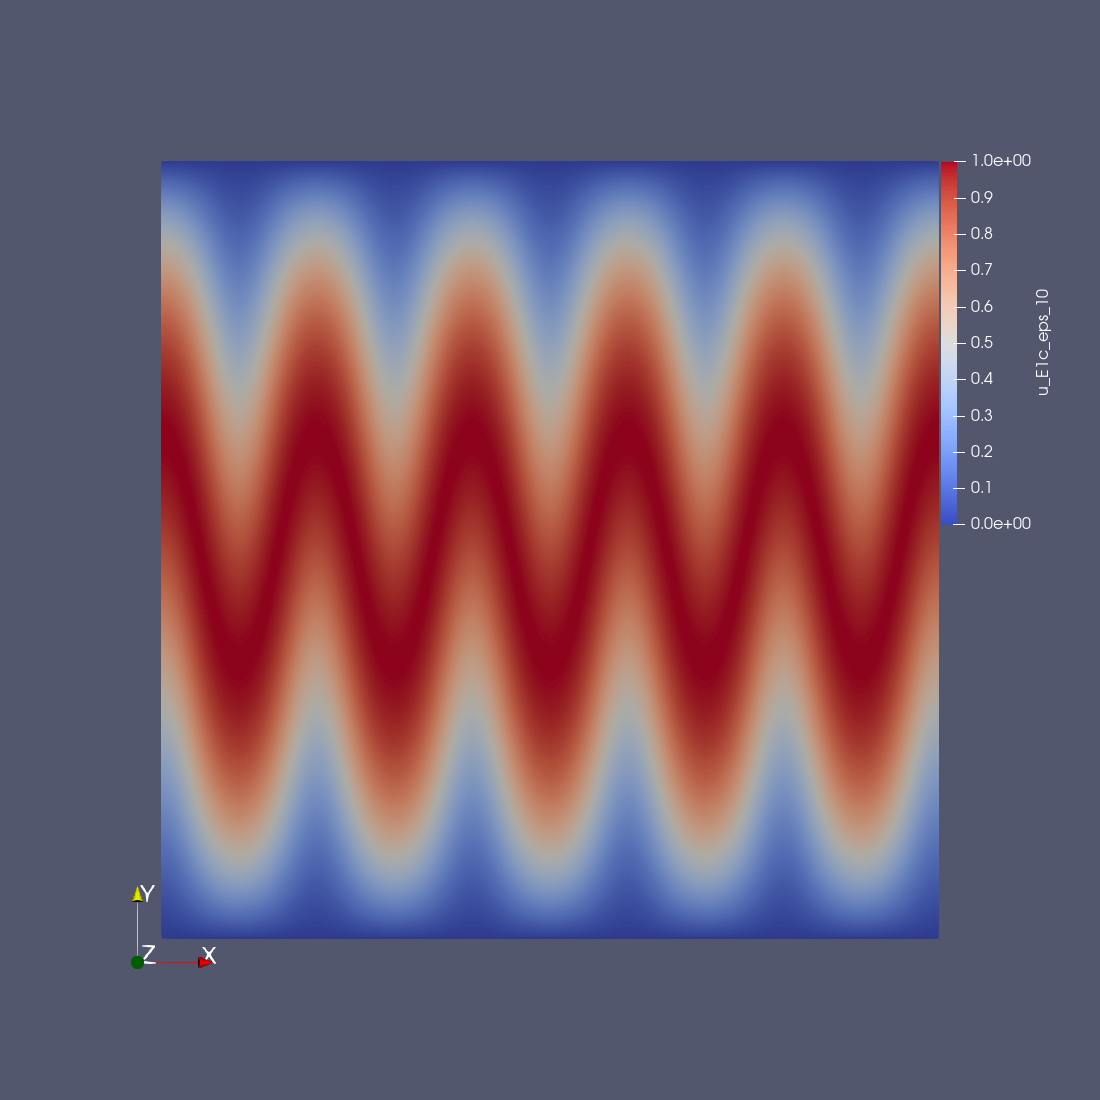
\includegraphics[width=\textwidth]{Pics/uf/u_E1c_eps_10.png}
     \caption{$\alpha=2, m=10$ and $\varepsilon = 10^{-10}$}
 \end{subfigure}
 \caption{Exact solution $u$ (\ref{E1_u}) for Example $1$.} \label{E1_us}
\end{figure}

\begin{figure}[H]
 \begin{subfigure}{0.5\textwidth}
     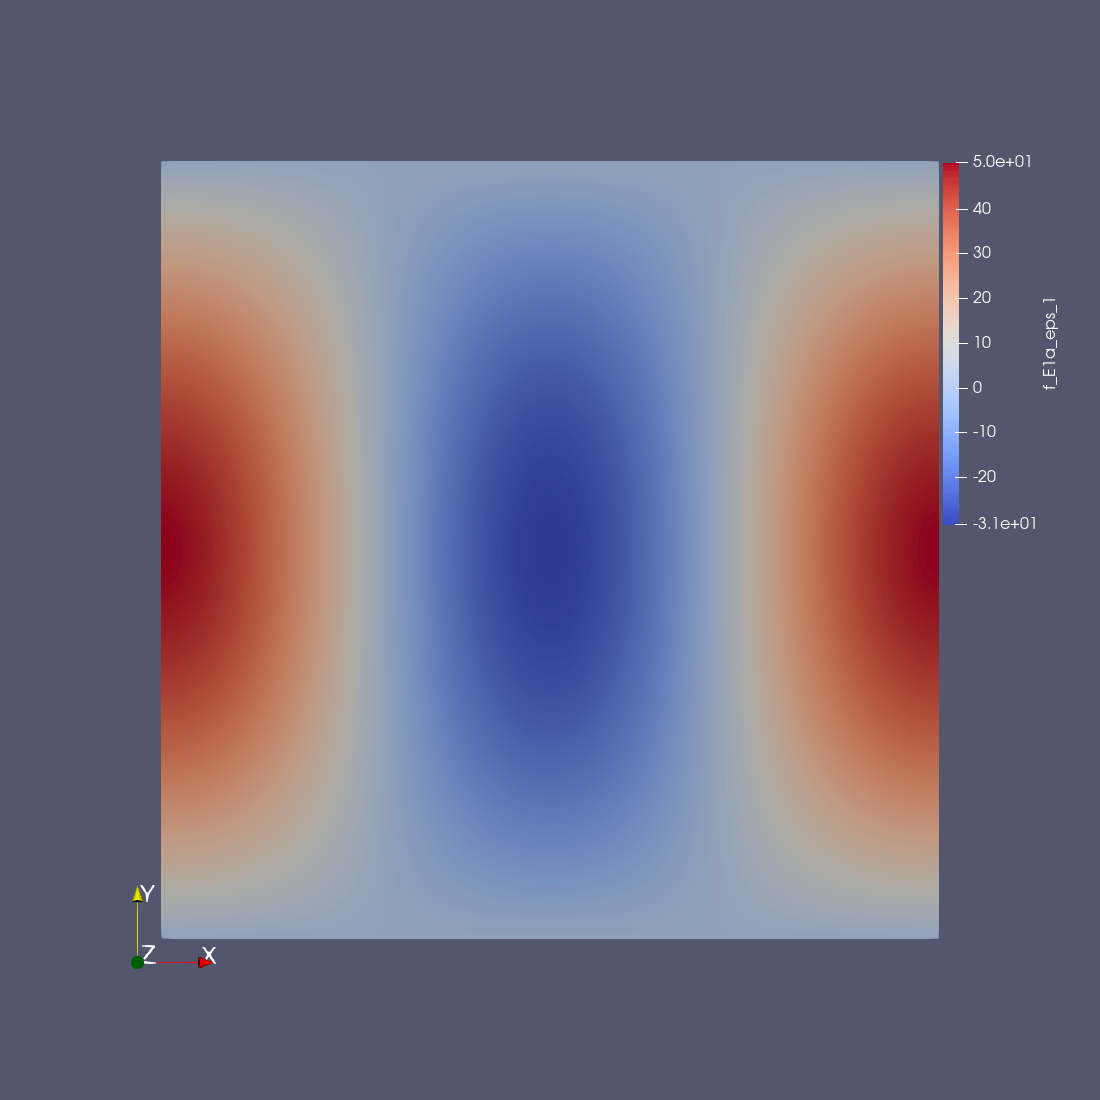
\includegraphics[width=\textwidth]{Pics/uf/F_E1a_eps1.png}
     \caption{$\alpha=0$ and $\varepsilon = 0.1$}
 \end{subfigure}
   \begin{subfigure}{0.5\textwidth}
     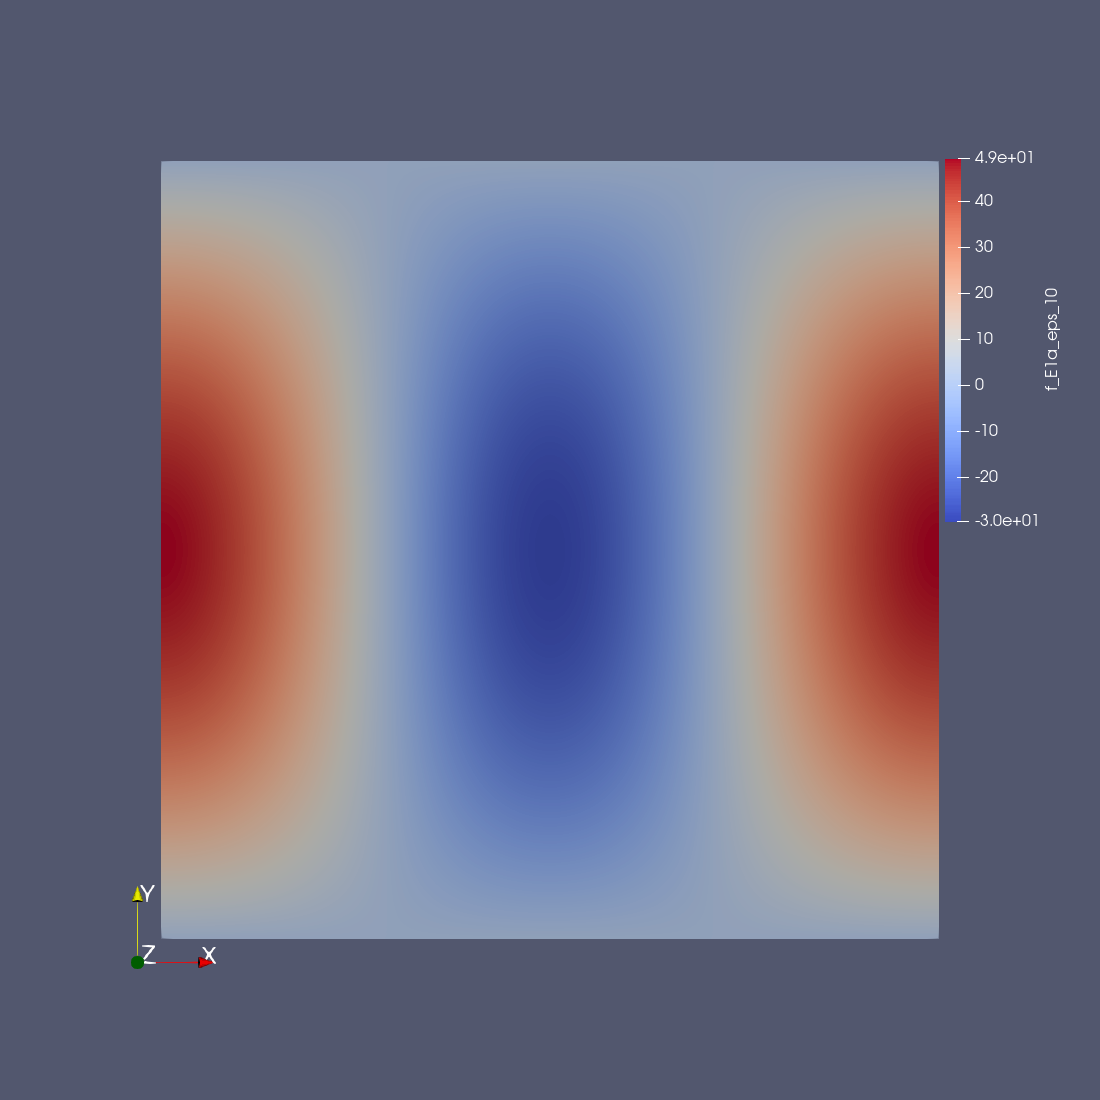
\includegraphics[width=\textwidth]{Pics/uf/F_E1a_eps10.png}
     \caption{$\alpha=0$ and $\varepsilon = 10^{-10}$}
 \end{subfigure}
 \begin{subfigure}{0.5\textwidth}
     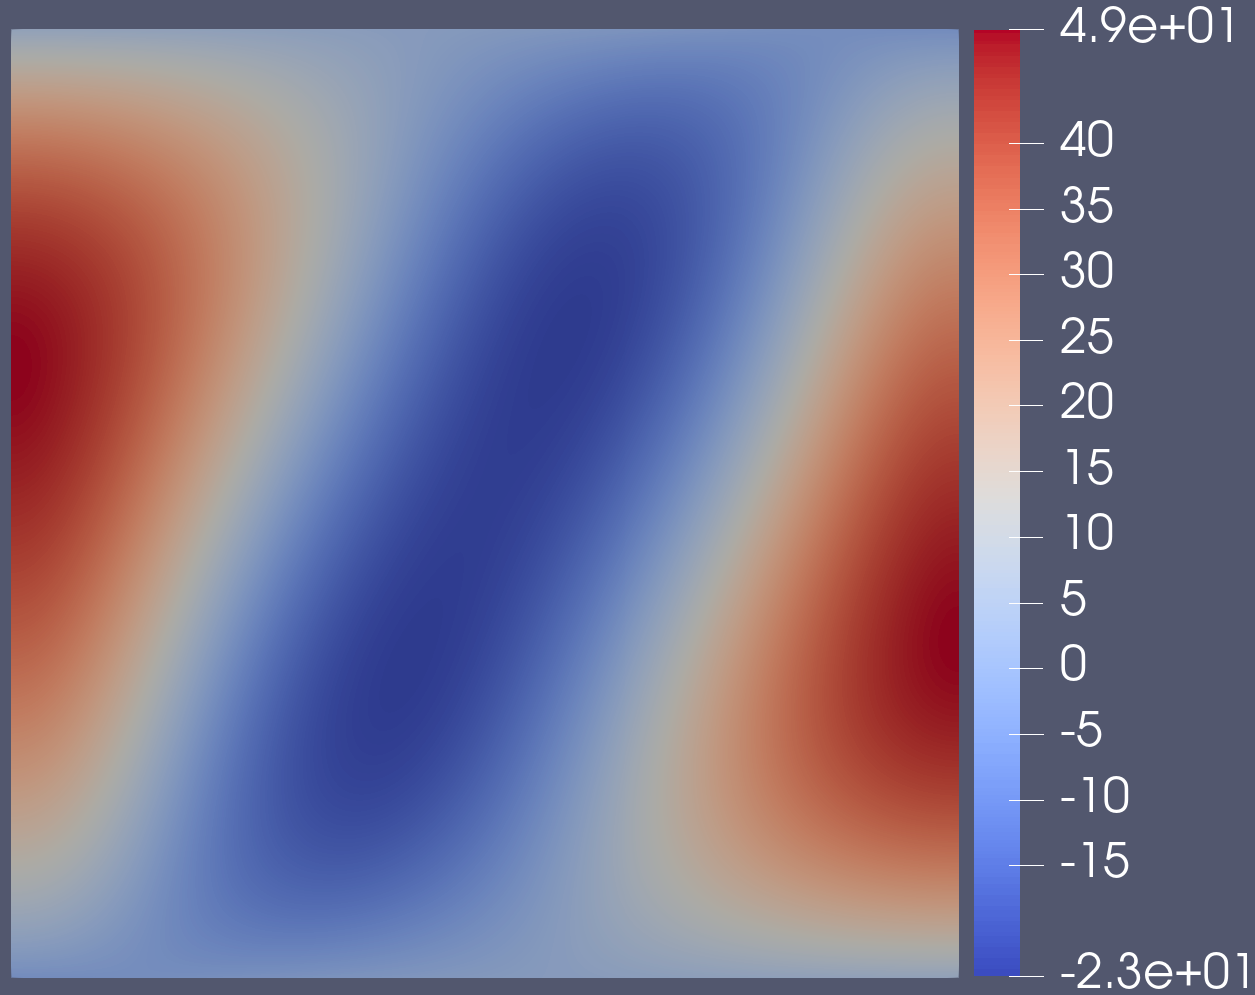
\includegraphics[width=\textwidth]{Pics/uf/F_E1b_eps1.png}
     \caption{$\alpha=2, m=1$ and $\varepsilon = 0.1$}
 \end{subfigure}
 \begin{subfigure}{0.5\textwidth}
     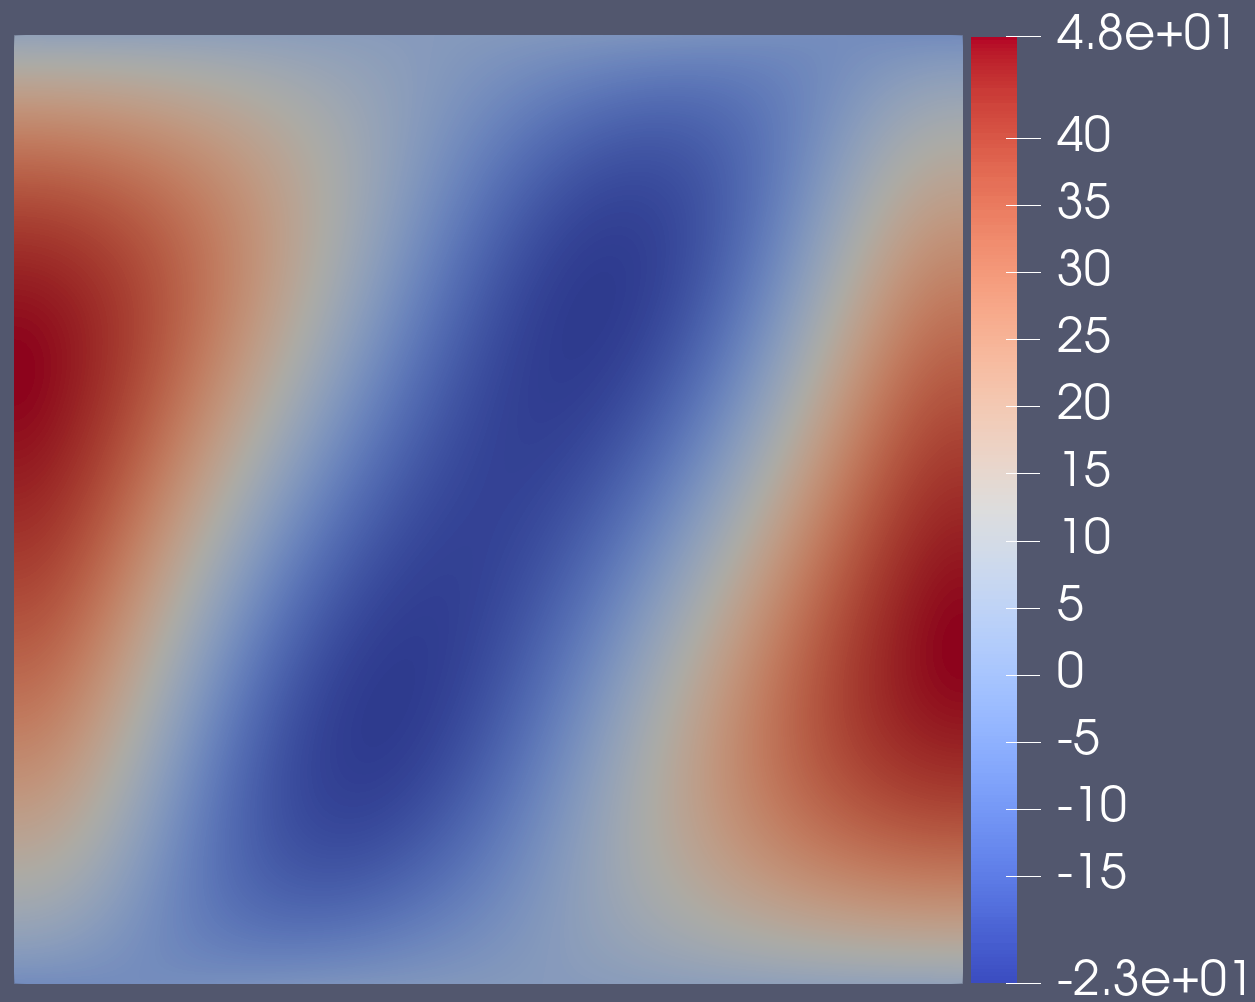
\includegraphics[width=\textwidth]{Pics/uf/F_E1b_eps_10.png}
     \caption{$\alpha=2, m=1$ and $\varepsilon = 10^{-10}$}
 \end{subfigure}
 \begin{subfigure}{0.5\textwidth}
     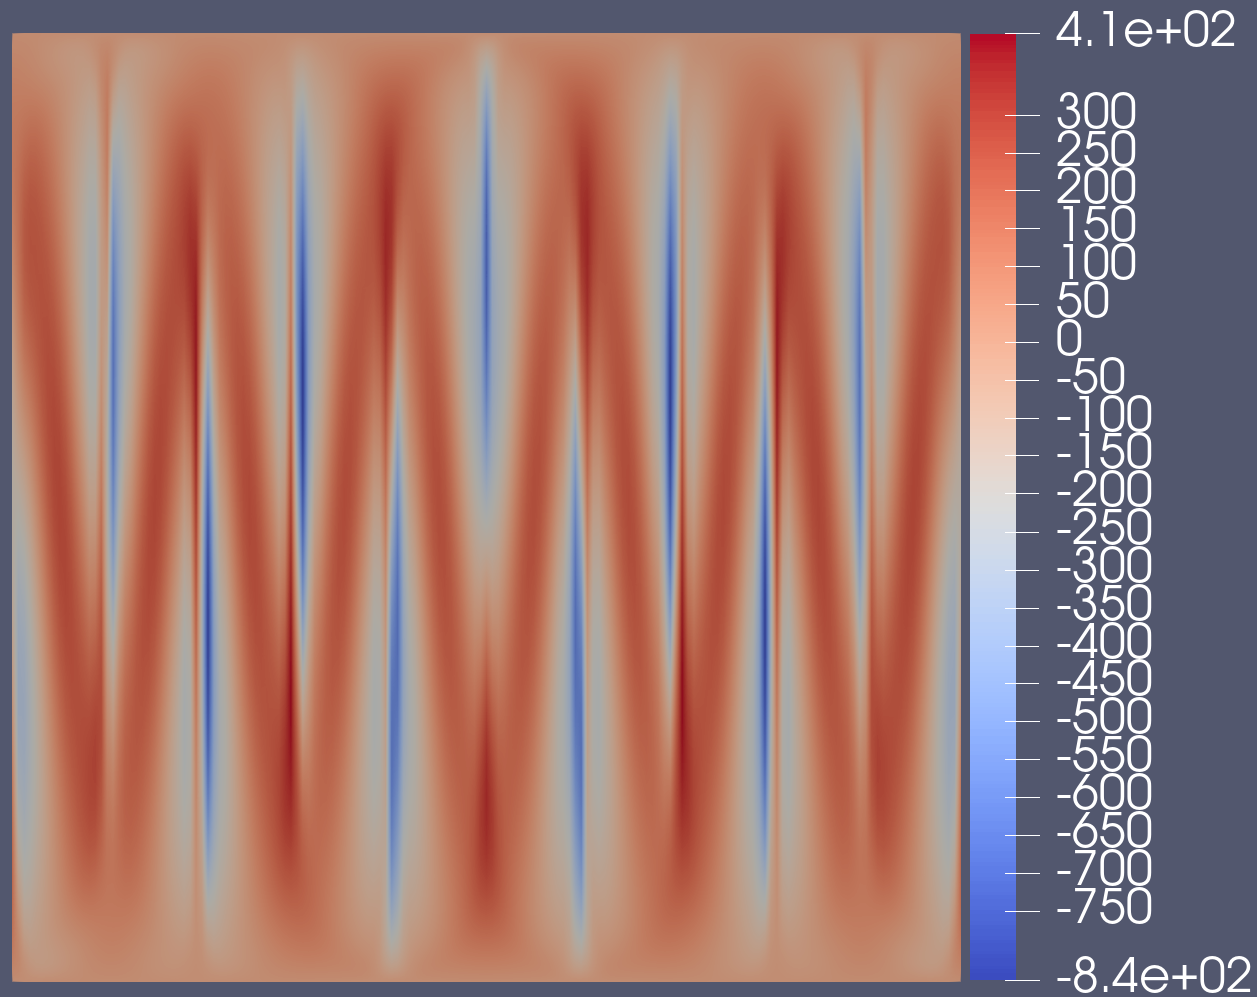
\includegraphics[width=\textwidth]{Pics/uf/F_E1c_eps_1.png}
     \caption{$\alpha=2, m=10$ and $\varepsilon = 0.1$}
 \end{subfigure}
 \hfill
 \begin{subfigure}{0.5\textwidth}
     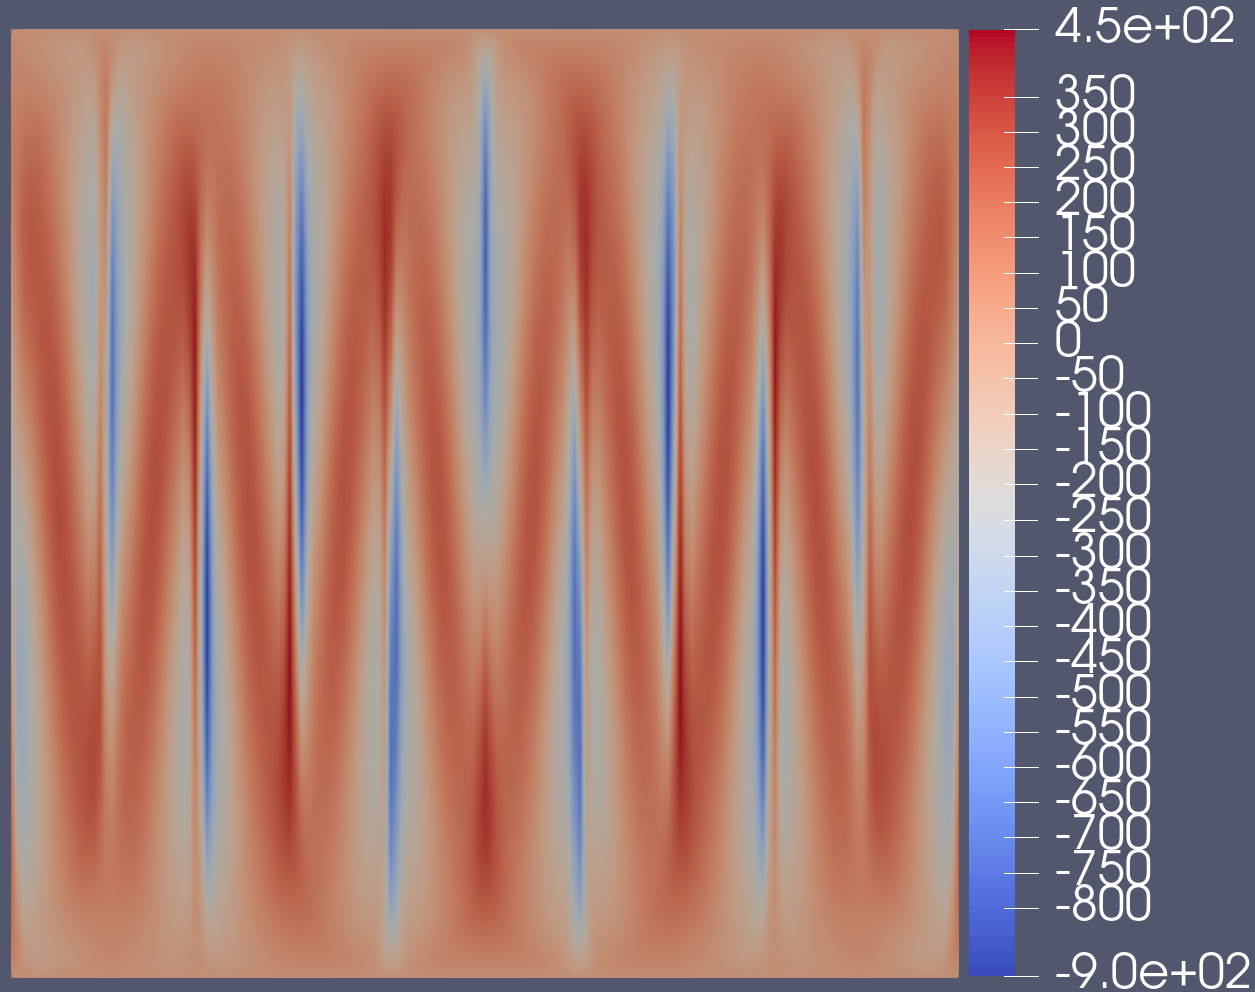
\includegraphics[width=\textwidth]{Pics/uf/f_E1c_eps_10.png}
     \caption{$\alpha=2, m=10$ and $\varepsilon = 10^{-10}$}
 \end{subfigure}
 \caption{Source term $f$ for Example $1$.} \label{E1_fs}
\end{figure}

\begin{figure}[H]
 \begin{subfigure}{0.42\textwidth}
     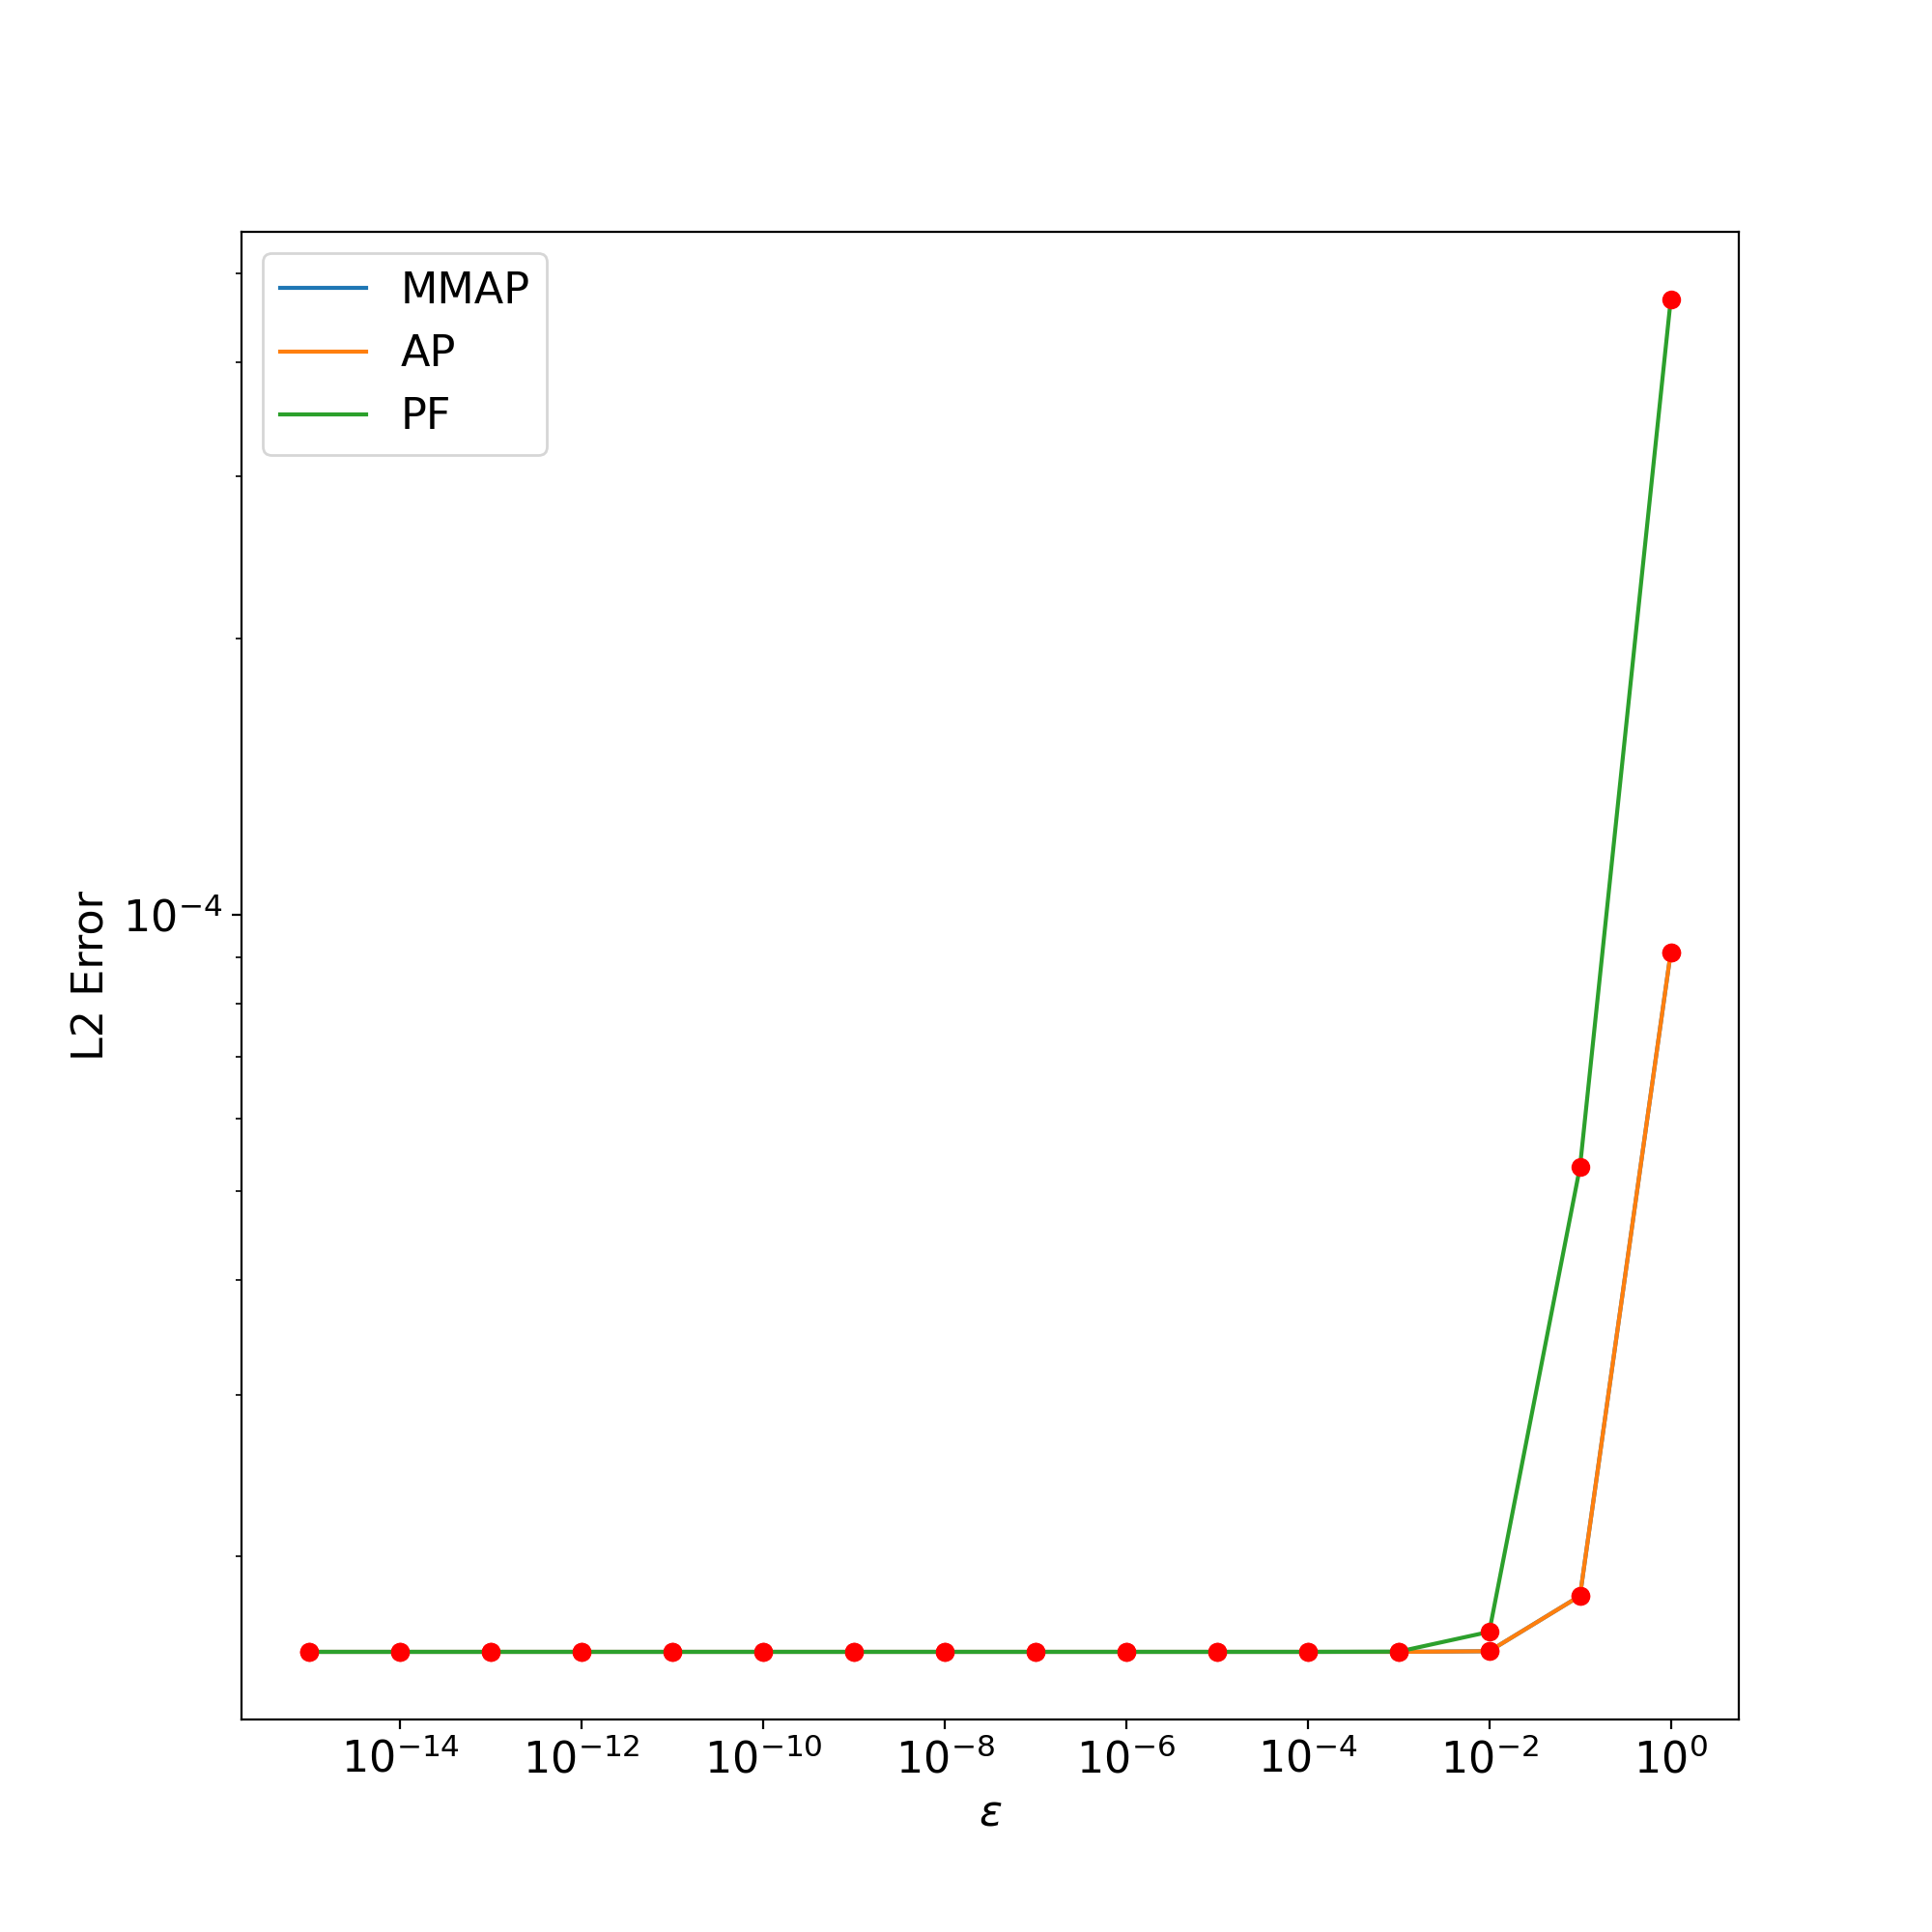
\includegraphics[width=\textwidth]{Pics/LHSims/E1a_MMAP_AP_PFL2.png}
     \caption{L2 Error $\alpha=0$}
 \end{subfigure}
   \begin{subfigure}{0.42\textwidth}
     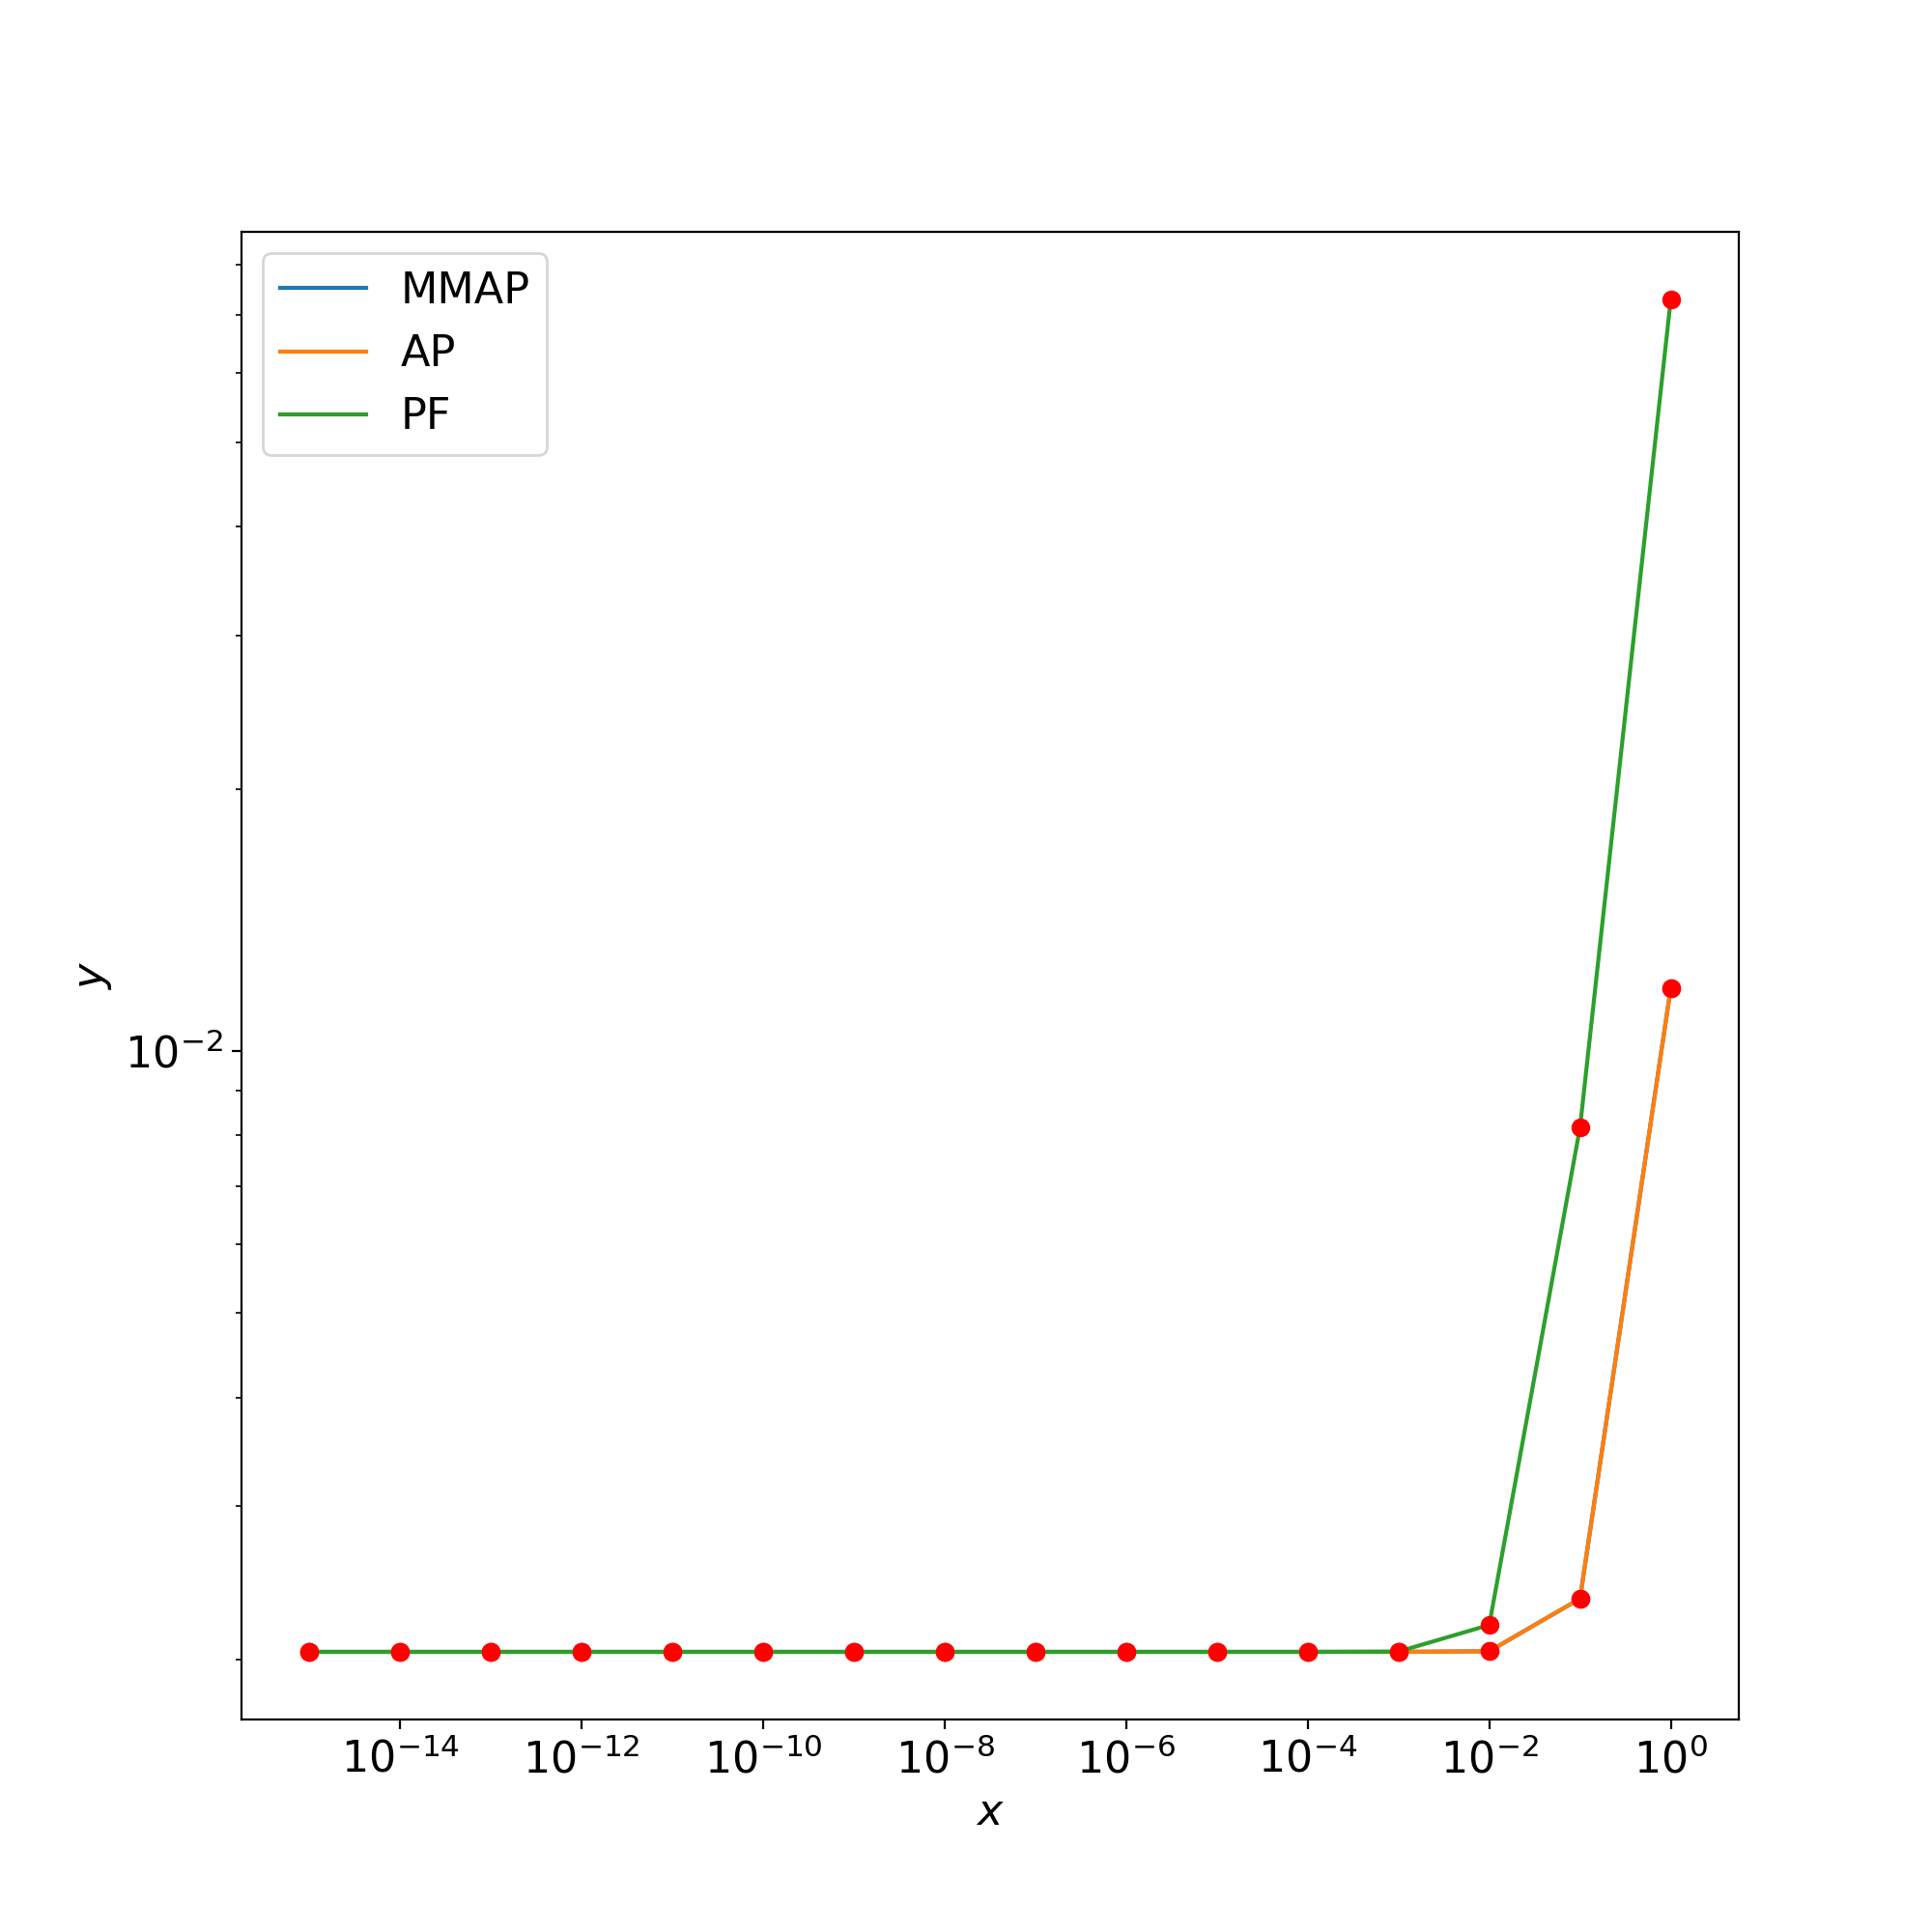
\includegraphics[width=\textwidth]{Pics/LHSims/E1a_MMAP_AP_PFH1.png}
     \caption{H1 Error $\alpha=0$}
 \end{subfigure}
 \begin{subfigure}{0.42\textwidth}
     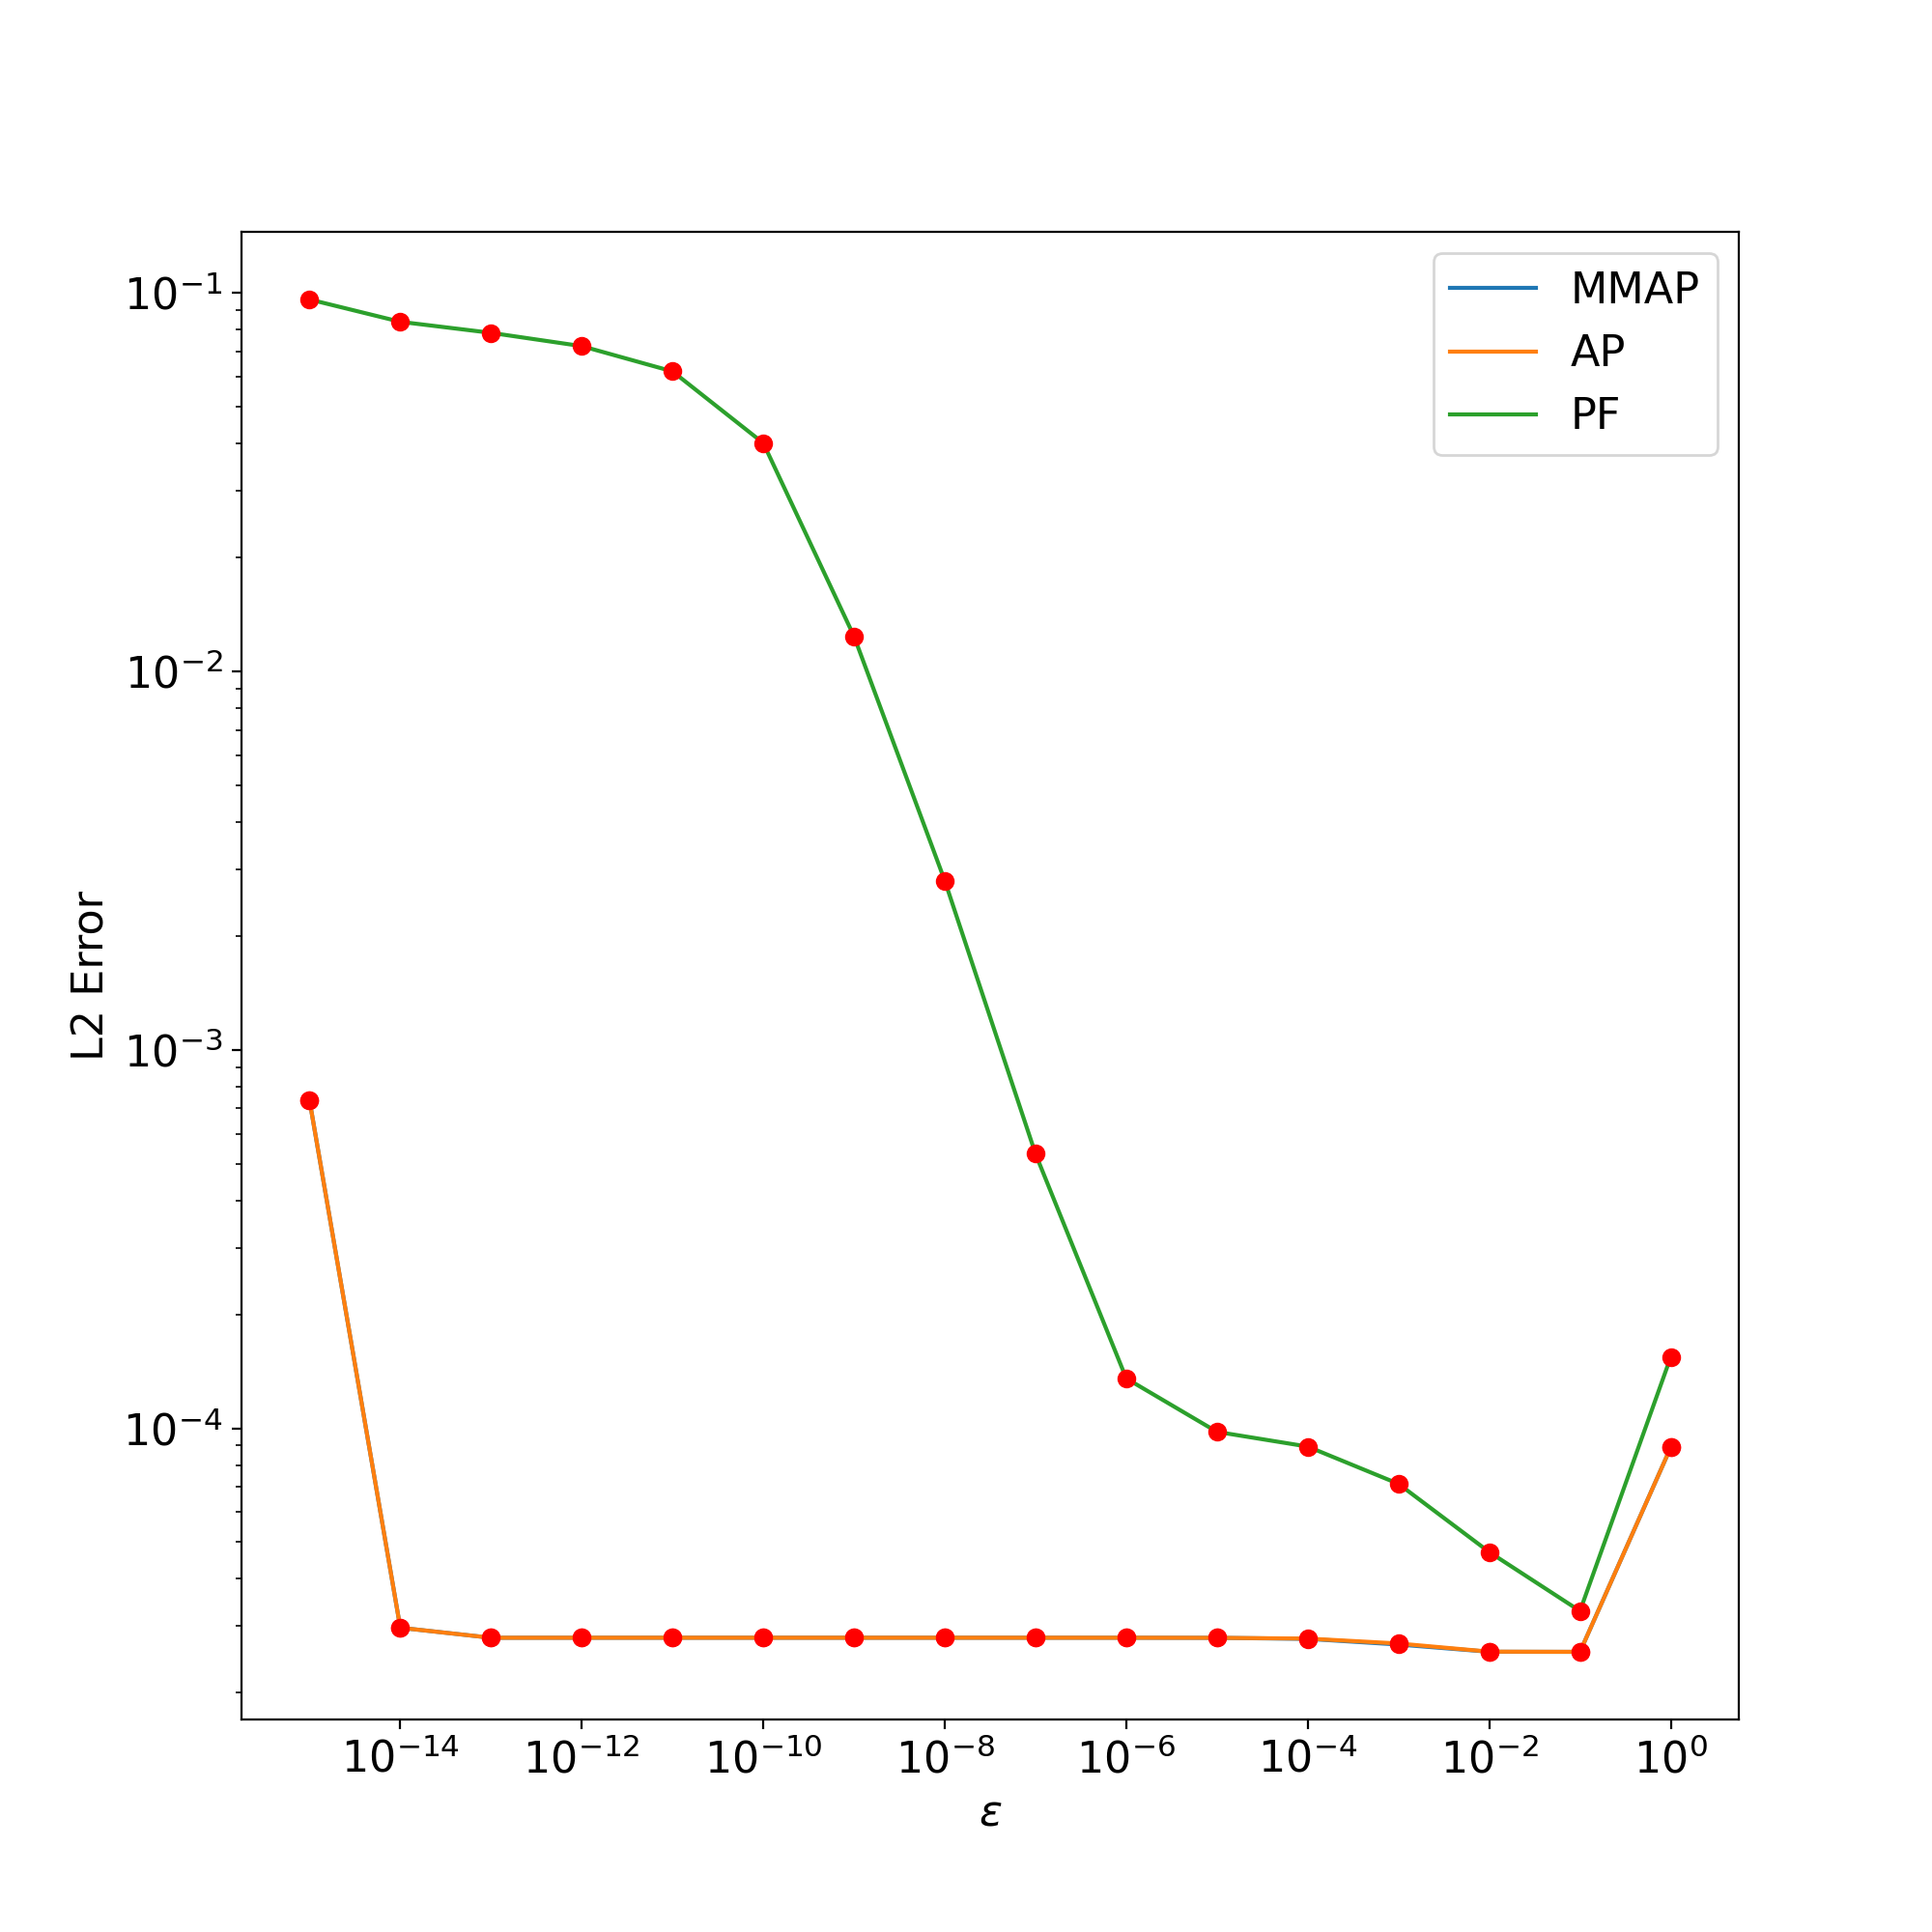
\includegraphics[width=\textwidth]{Pics/LHSims/E1b_MMAP_AP_PFL2.png}
     \caption{L2 Error $\alpha=2, m=1$} \label{E1_Mild_Ans}
 \end{subfigure}
 \begin{subfigure}{0.42\textwidth}
     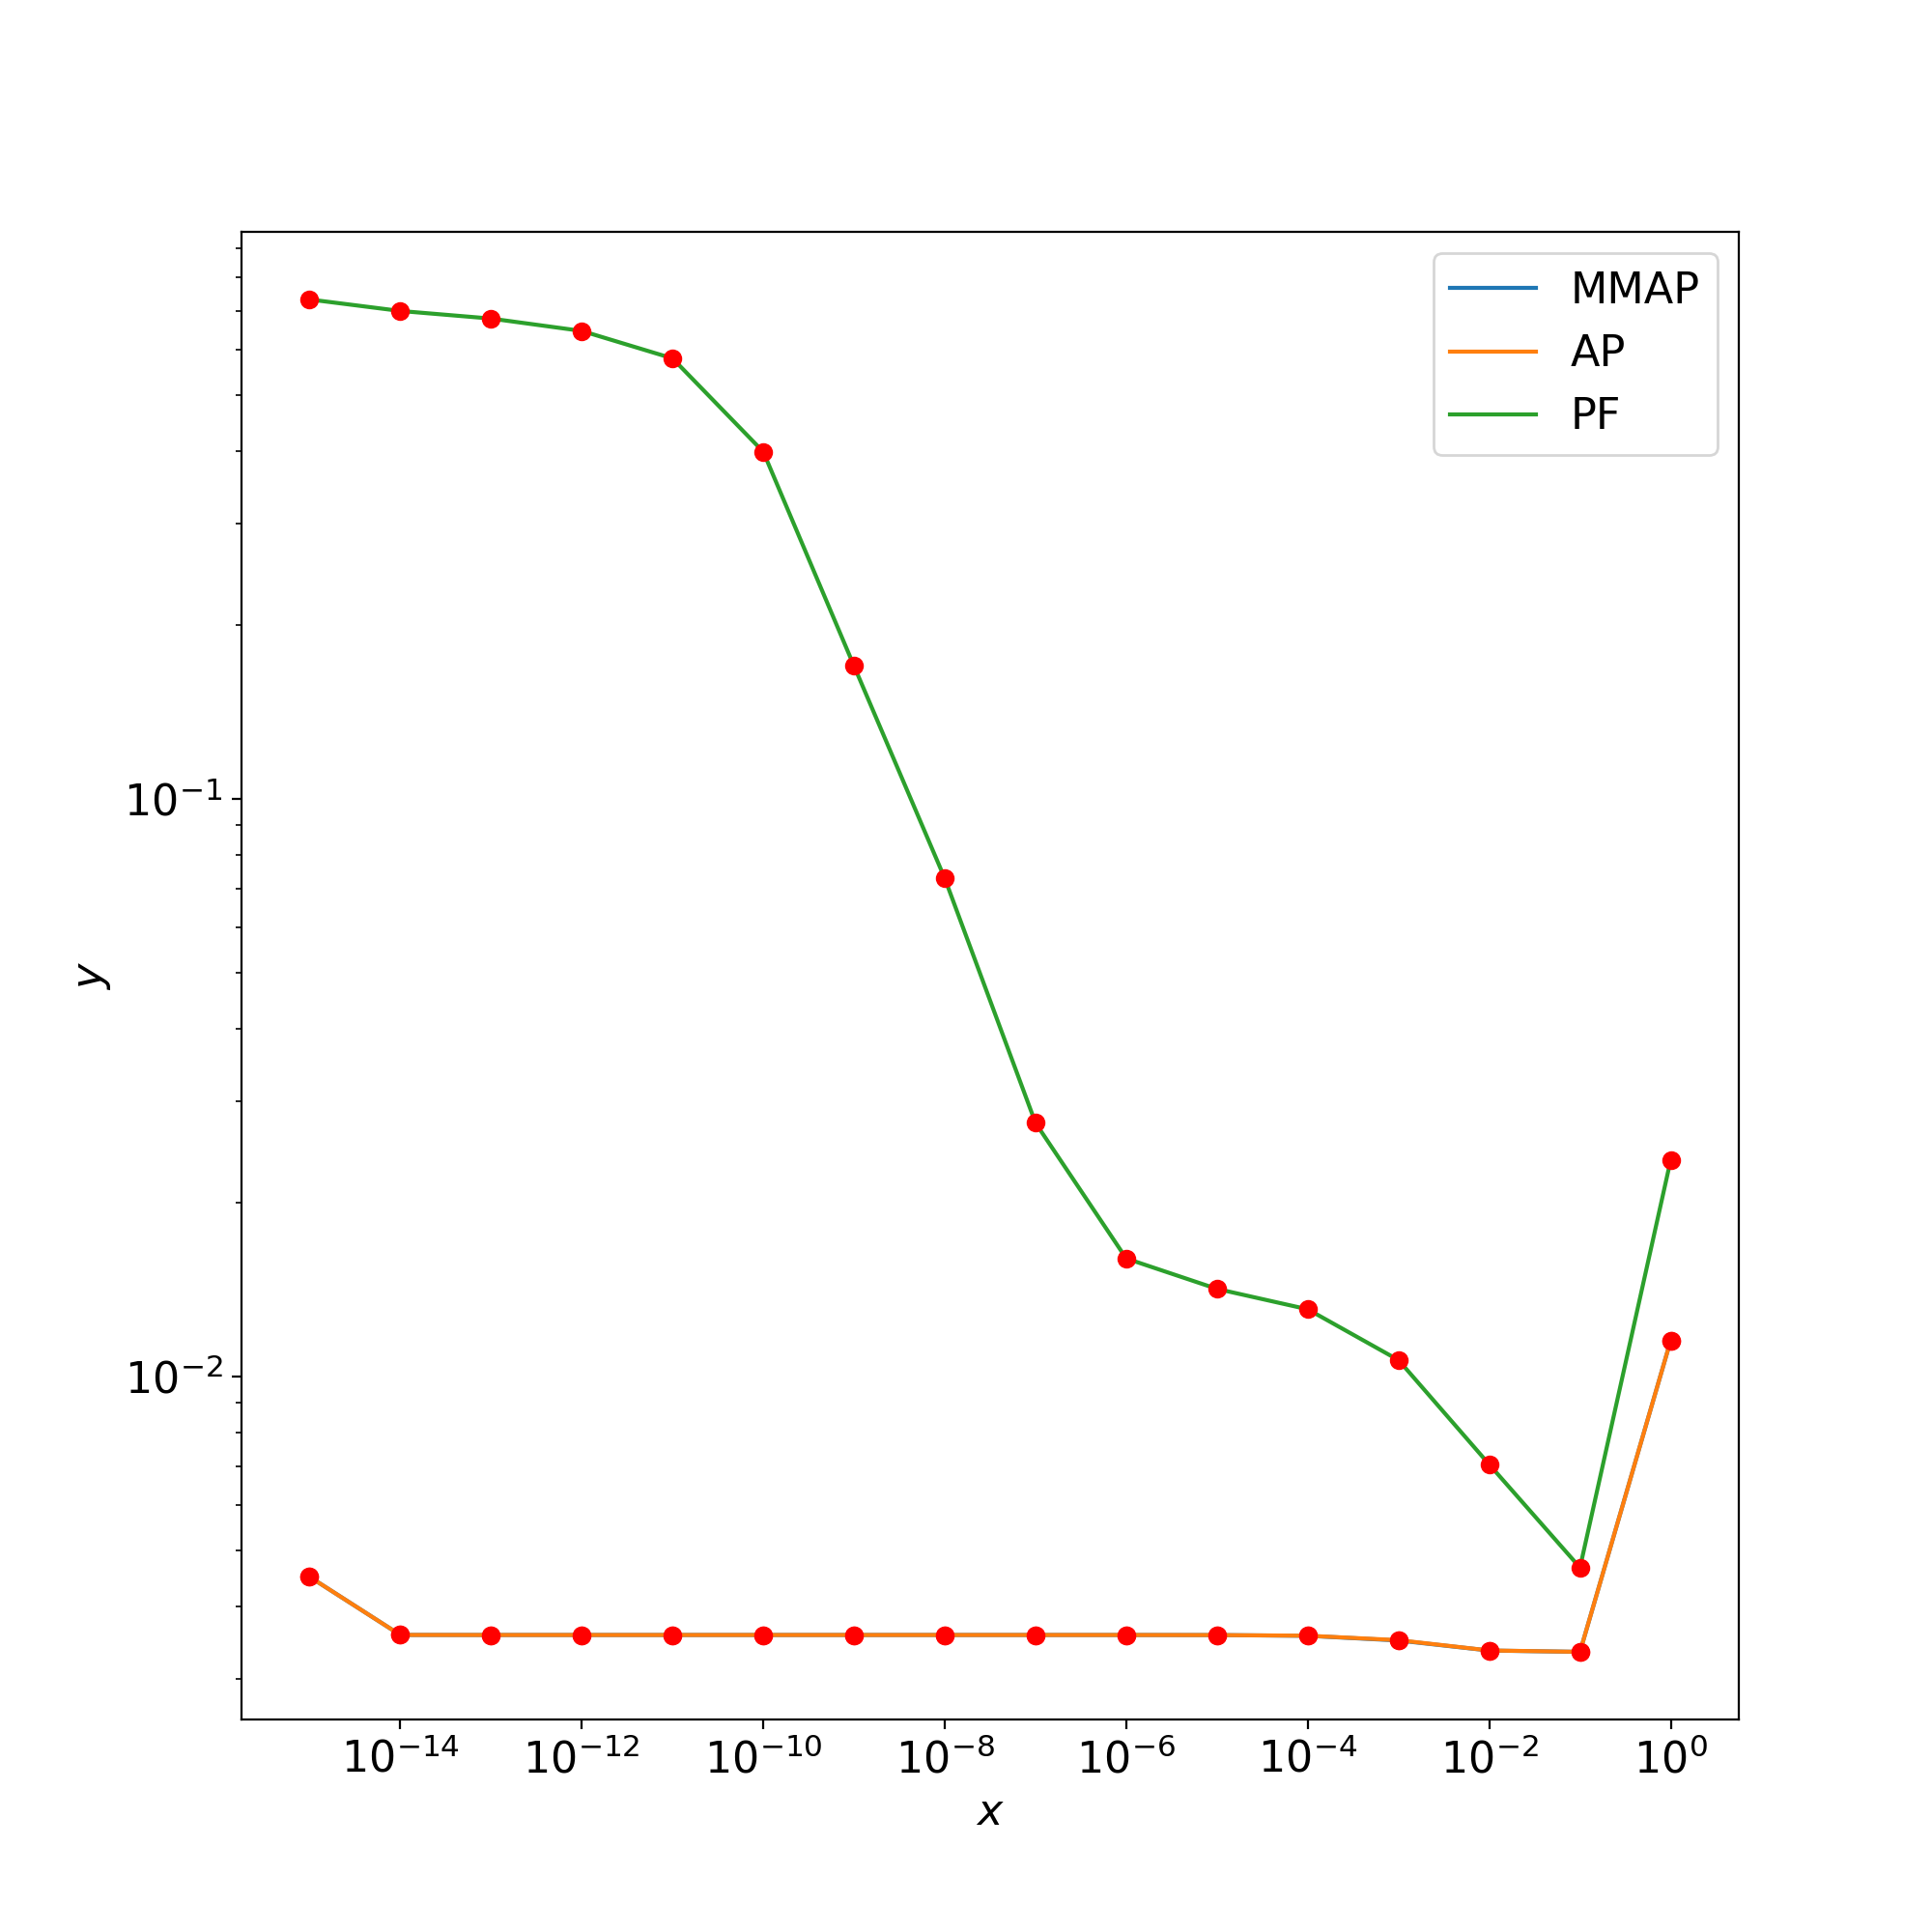
\includegraphics[width=\textwidth]{Pics/LHSims/E1b_MMAP_AP_PFH1.png}
     \caption{H1 Error, $\alpha=2, m=1$}
 \end{subfigure}
 \begin{subfigure}{0.42\textwidth}
     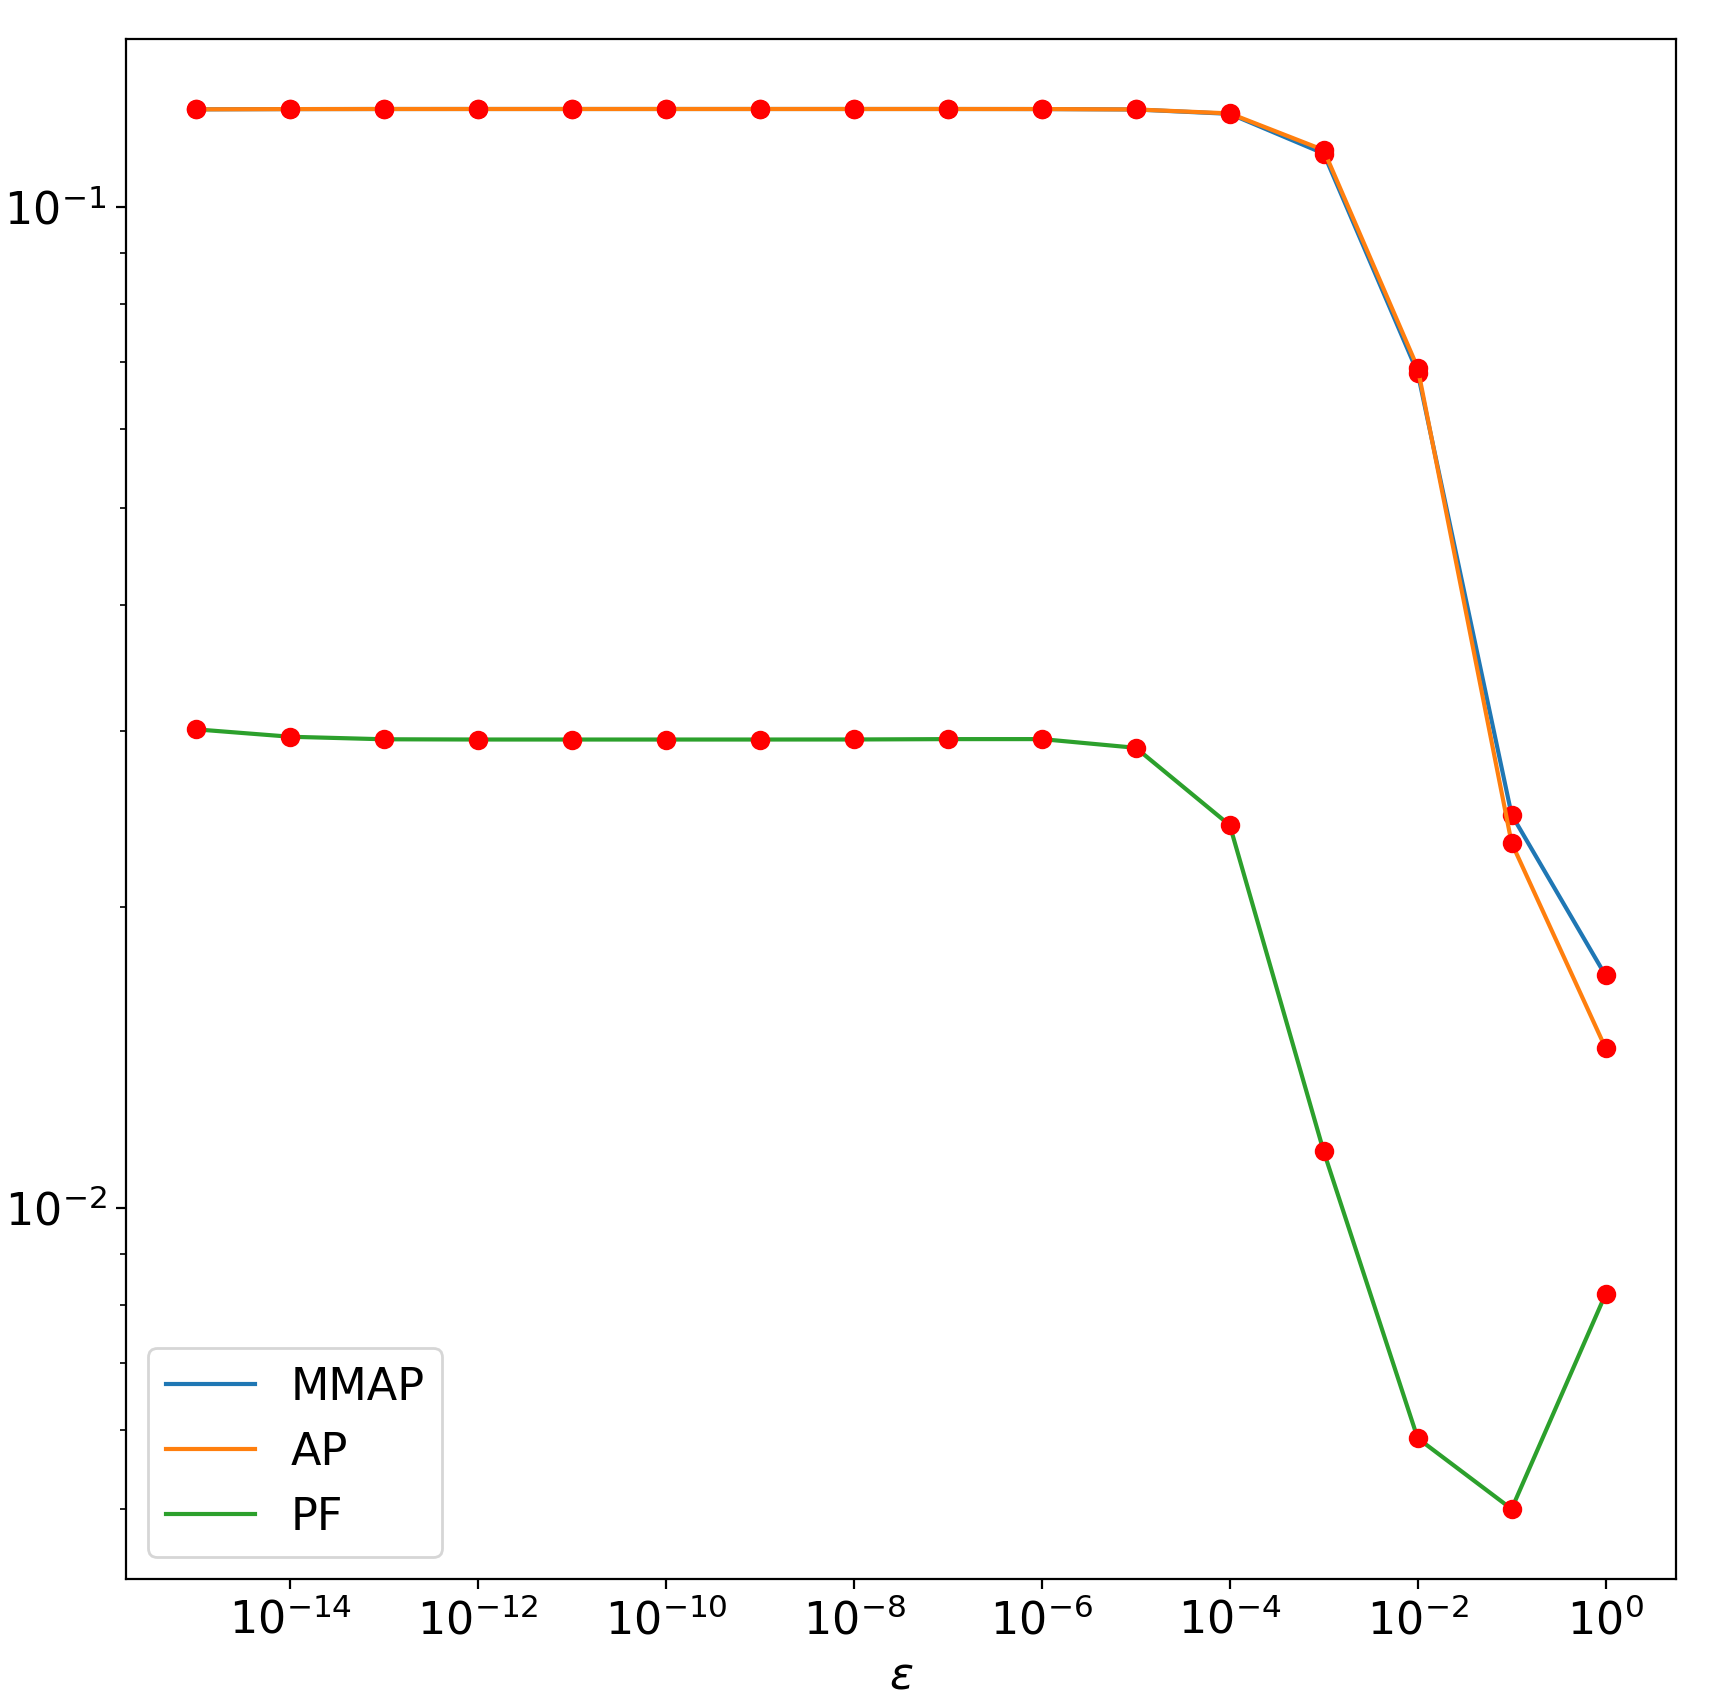
\includegraphics[width=\textwidth]{Pics/LHSims/E1c_MMAP_AP_PFL2.png}
     \caption{L2 Error, $\alpha=2, m=10$} \label{E1_Strong_Ans}
 \end{subfigure}
 \hfill
 \begin{subfigure}{0.42\textwidth}
     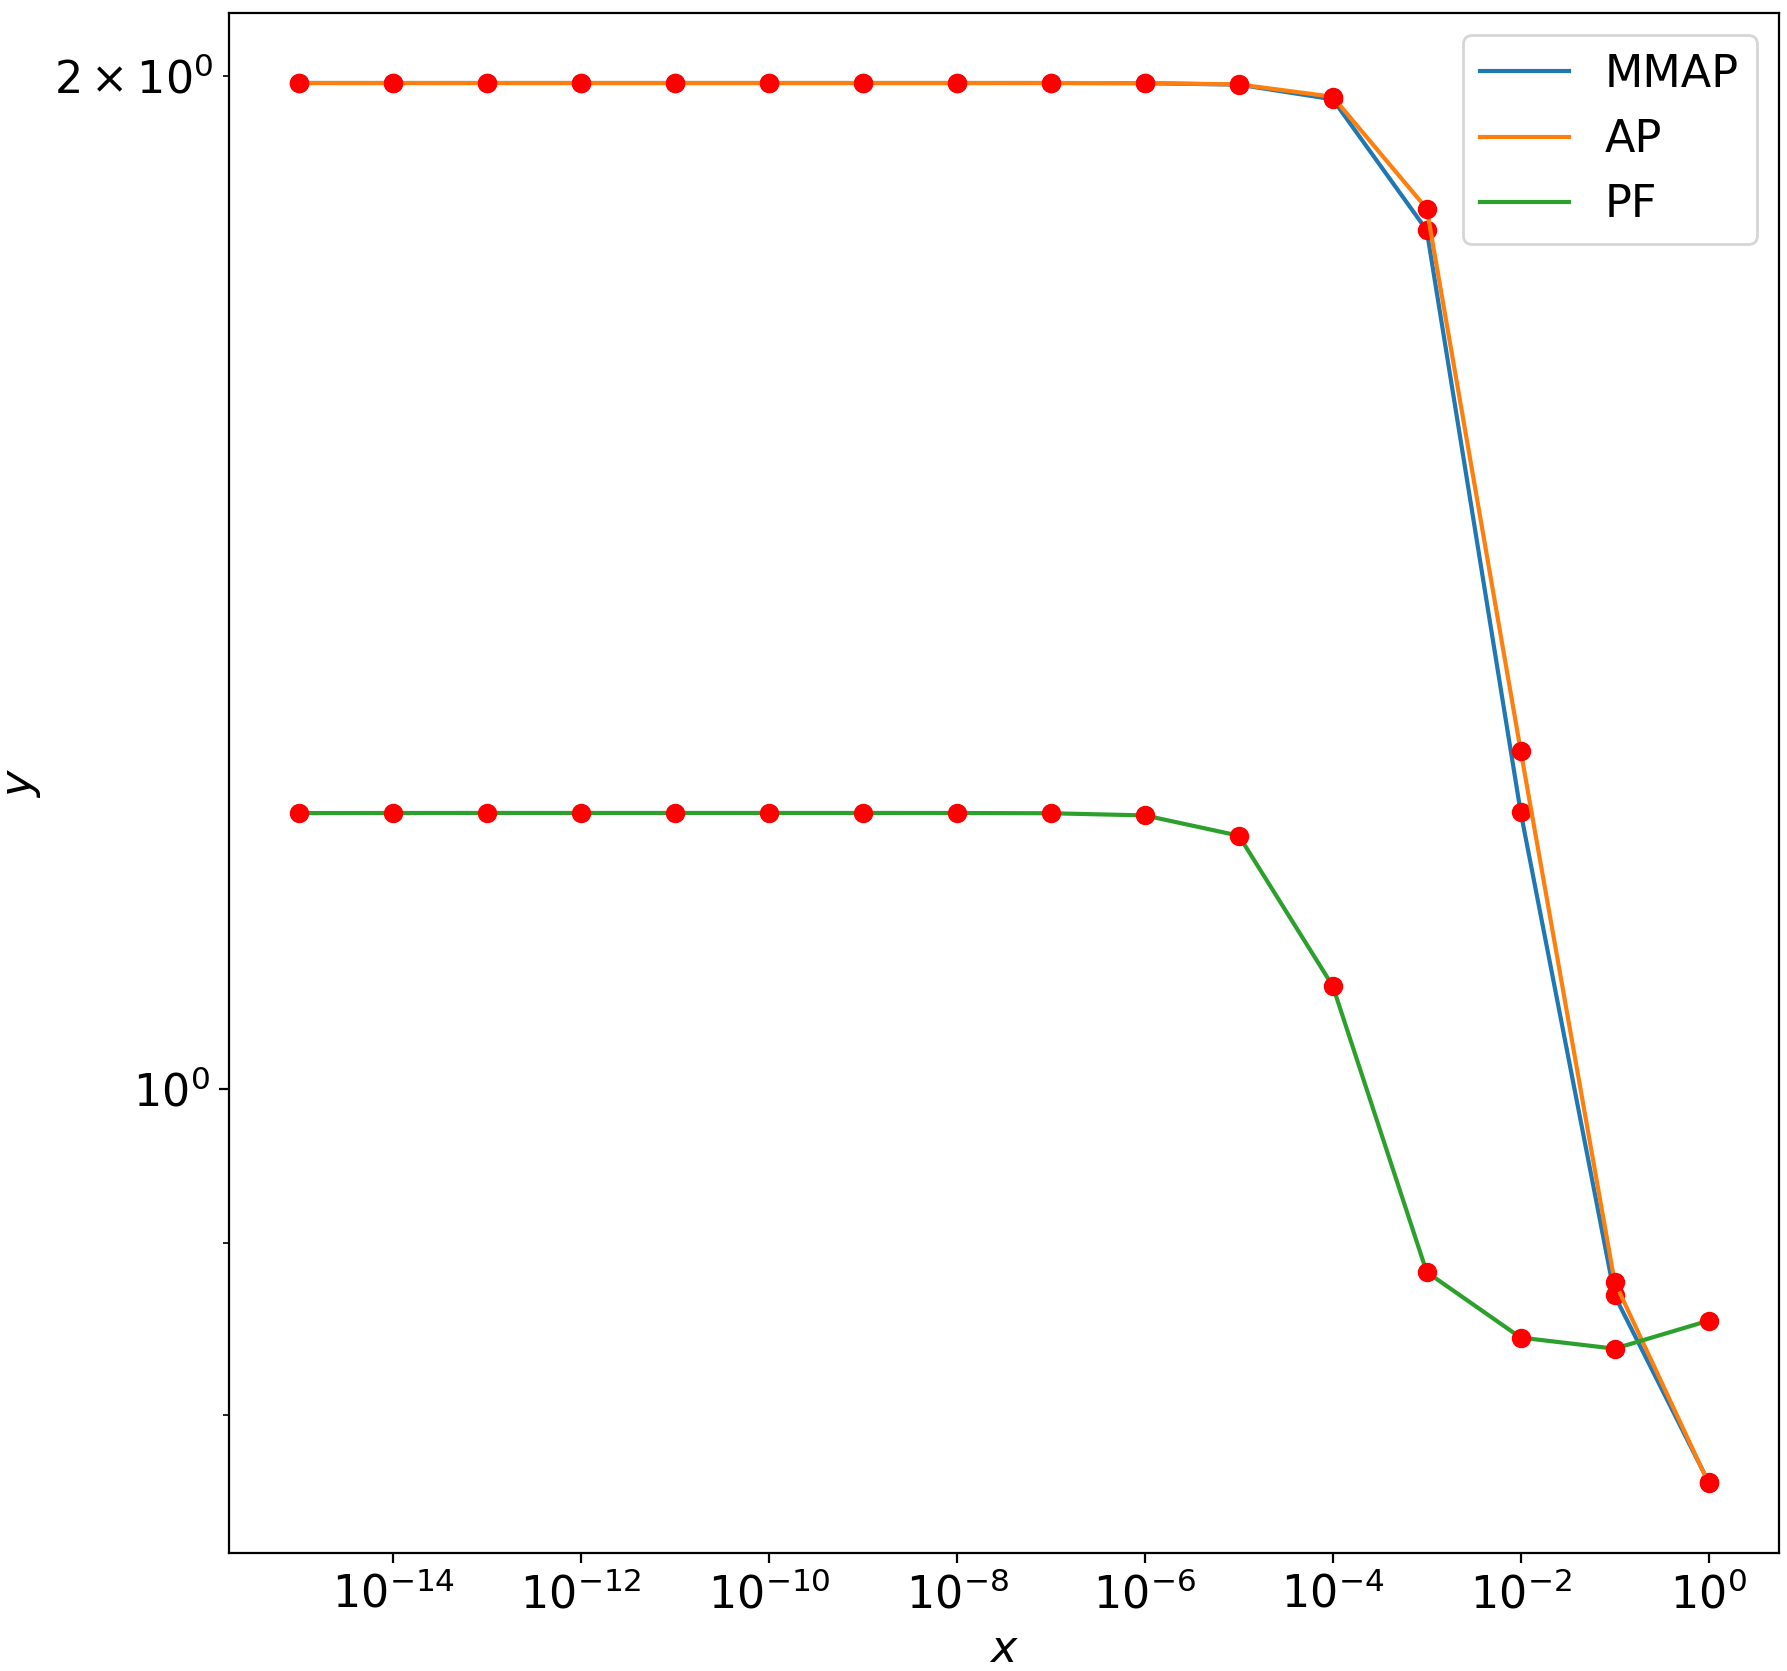
\includegraphics[width=\textwidth]{Pics/LHSims/E1c_MMAP_AP_PFH1.png}
     \caption{H1 Error, $\alpha=2, m=10$}
 \end{subfigure}
 \caption{Numerical demonstration for solver $MMAP, AP$ and $PF$ on a $20\times 20$ quadrilateral grid using CG order $2$ for Example $1$, with $x=\varepsilon$ and $y=$ Error.} \label{E1_LH_PF}
\end{figure}

\begin{figure}[H]
 \begin{subfigure}{0.42\textwidth}
     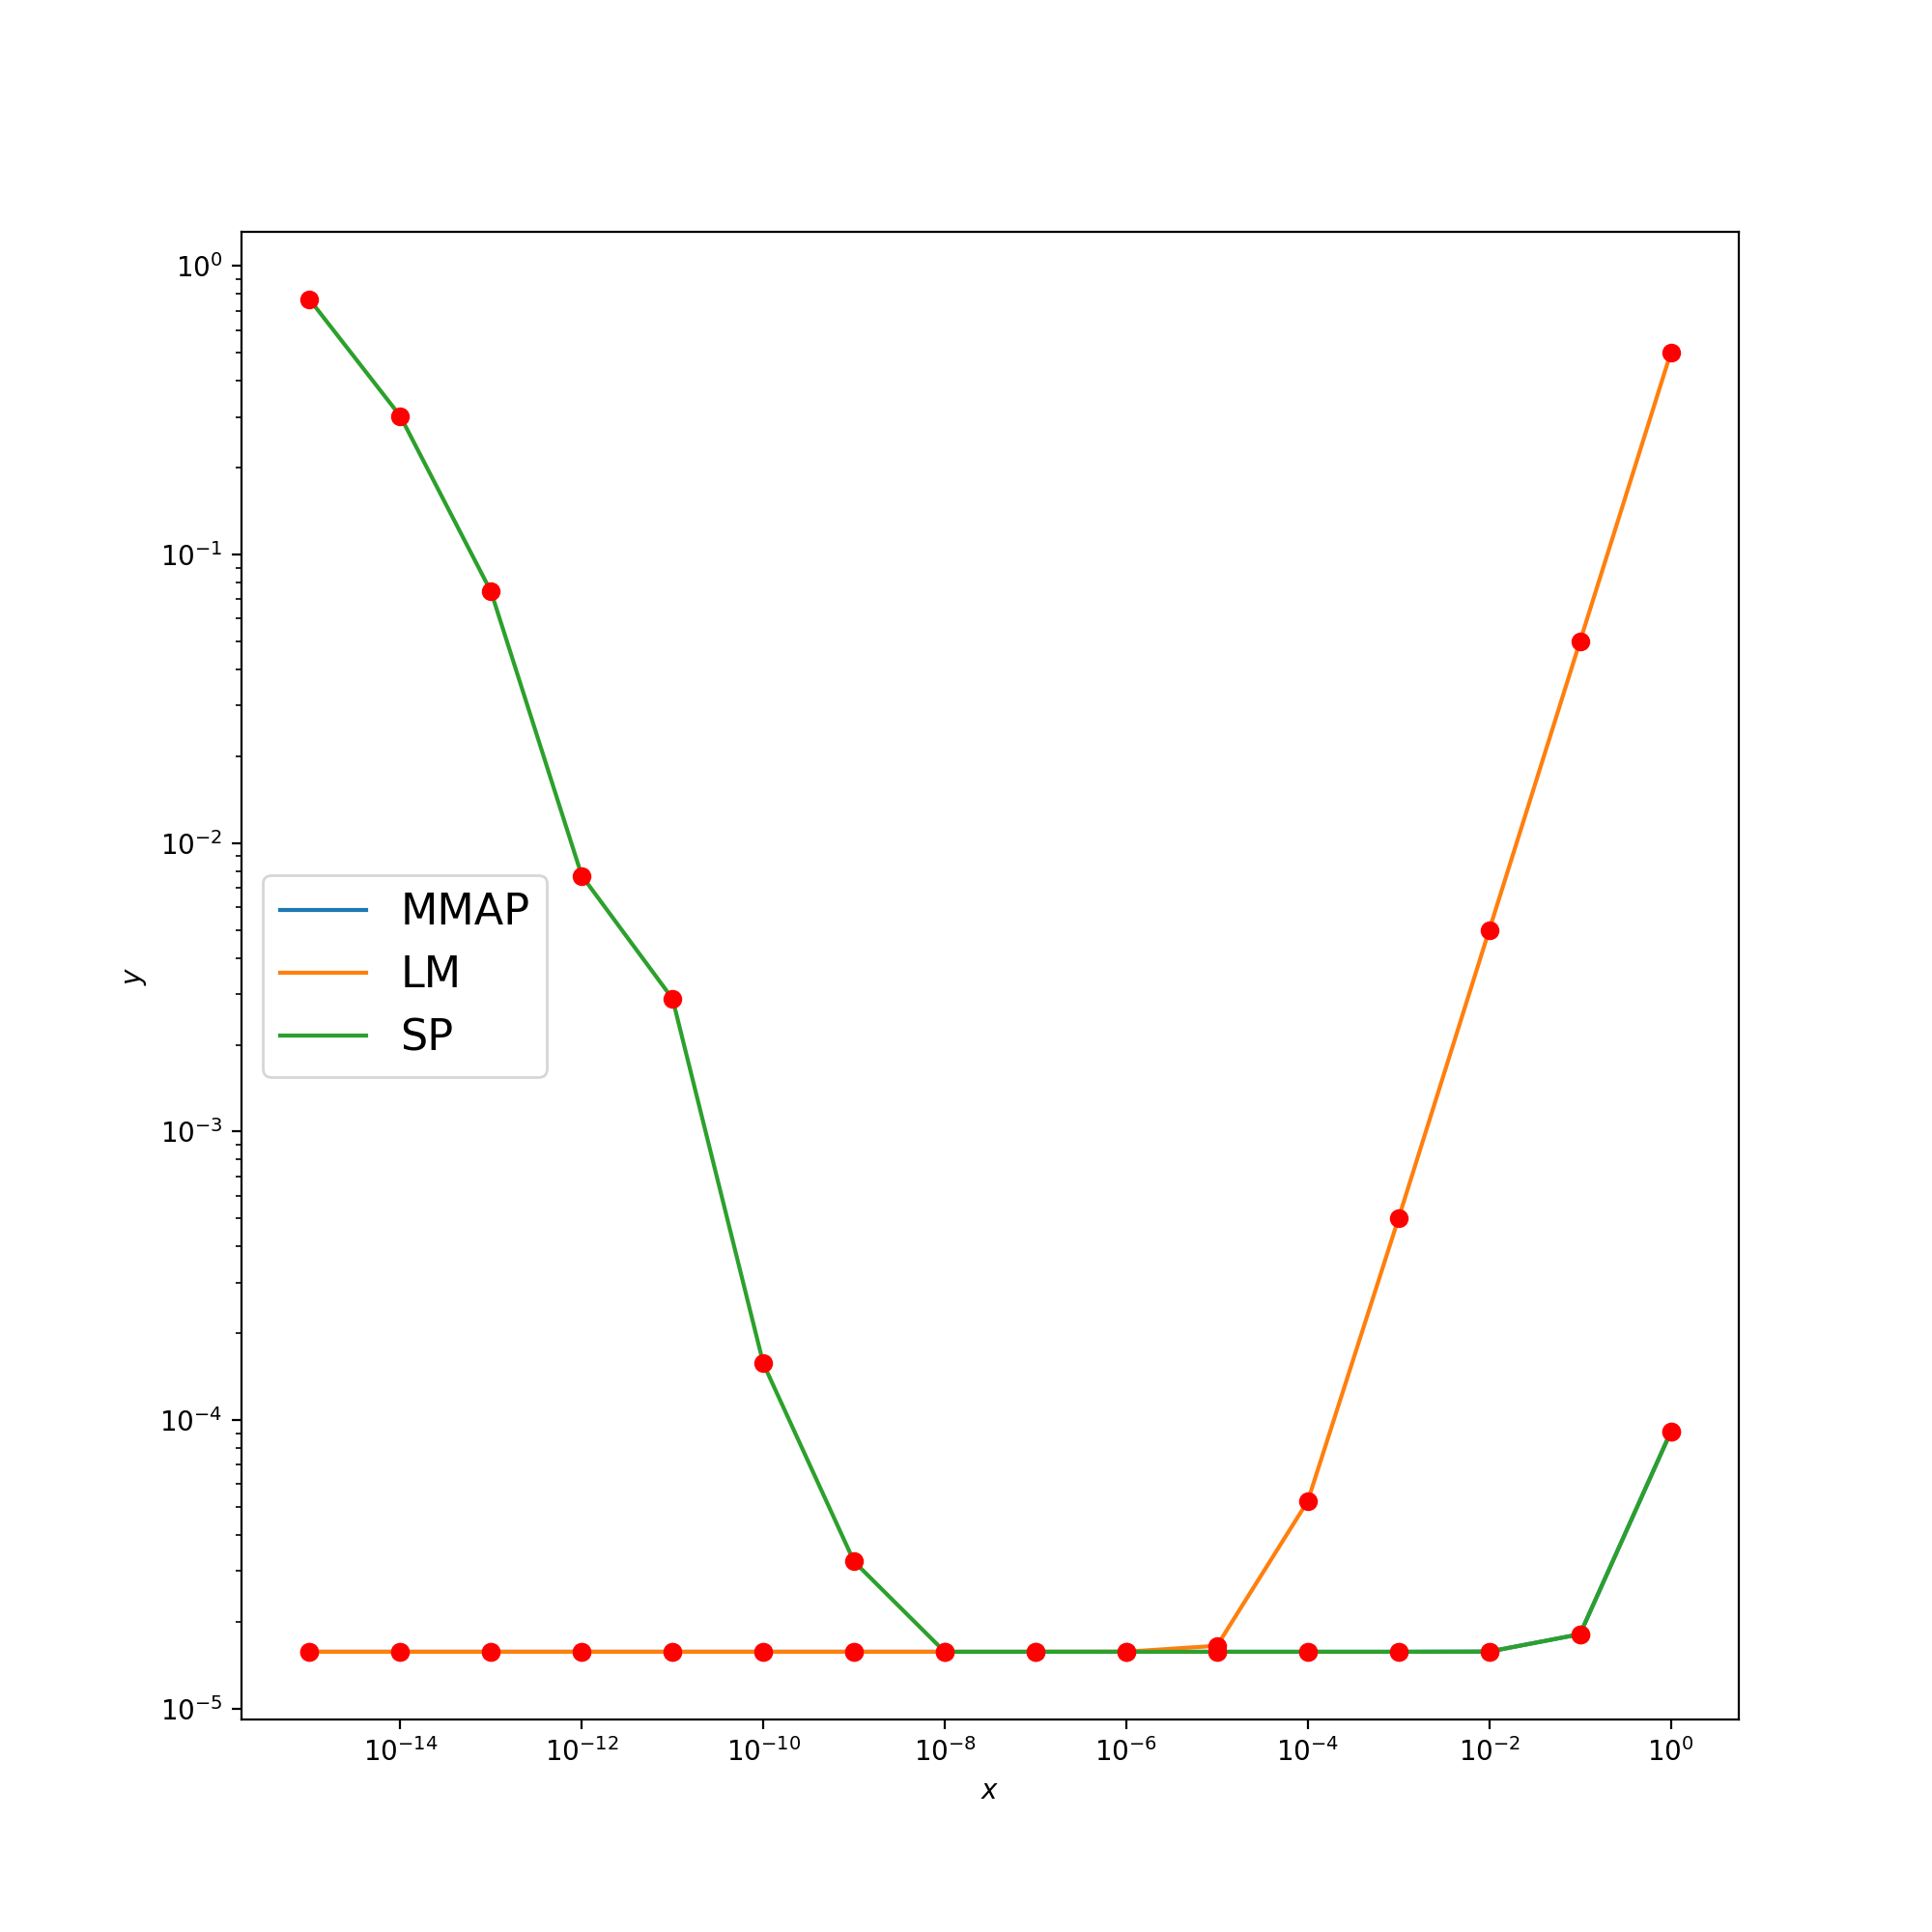
\includegraphics[width=\textwidth]{Pics/LHSims/E1a_MMAP_LM_SPL2.png}
     \caption{L2 Error $\alpha=0$}
 \end{subfigure}
   \begin{subfigure}{0.42\textwidth}
     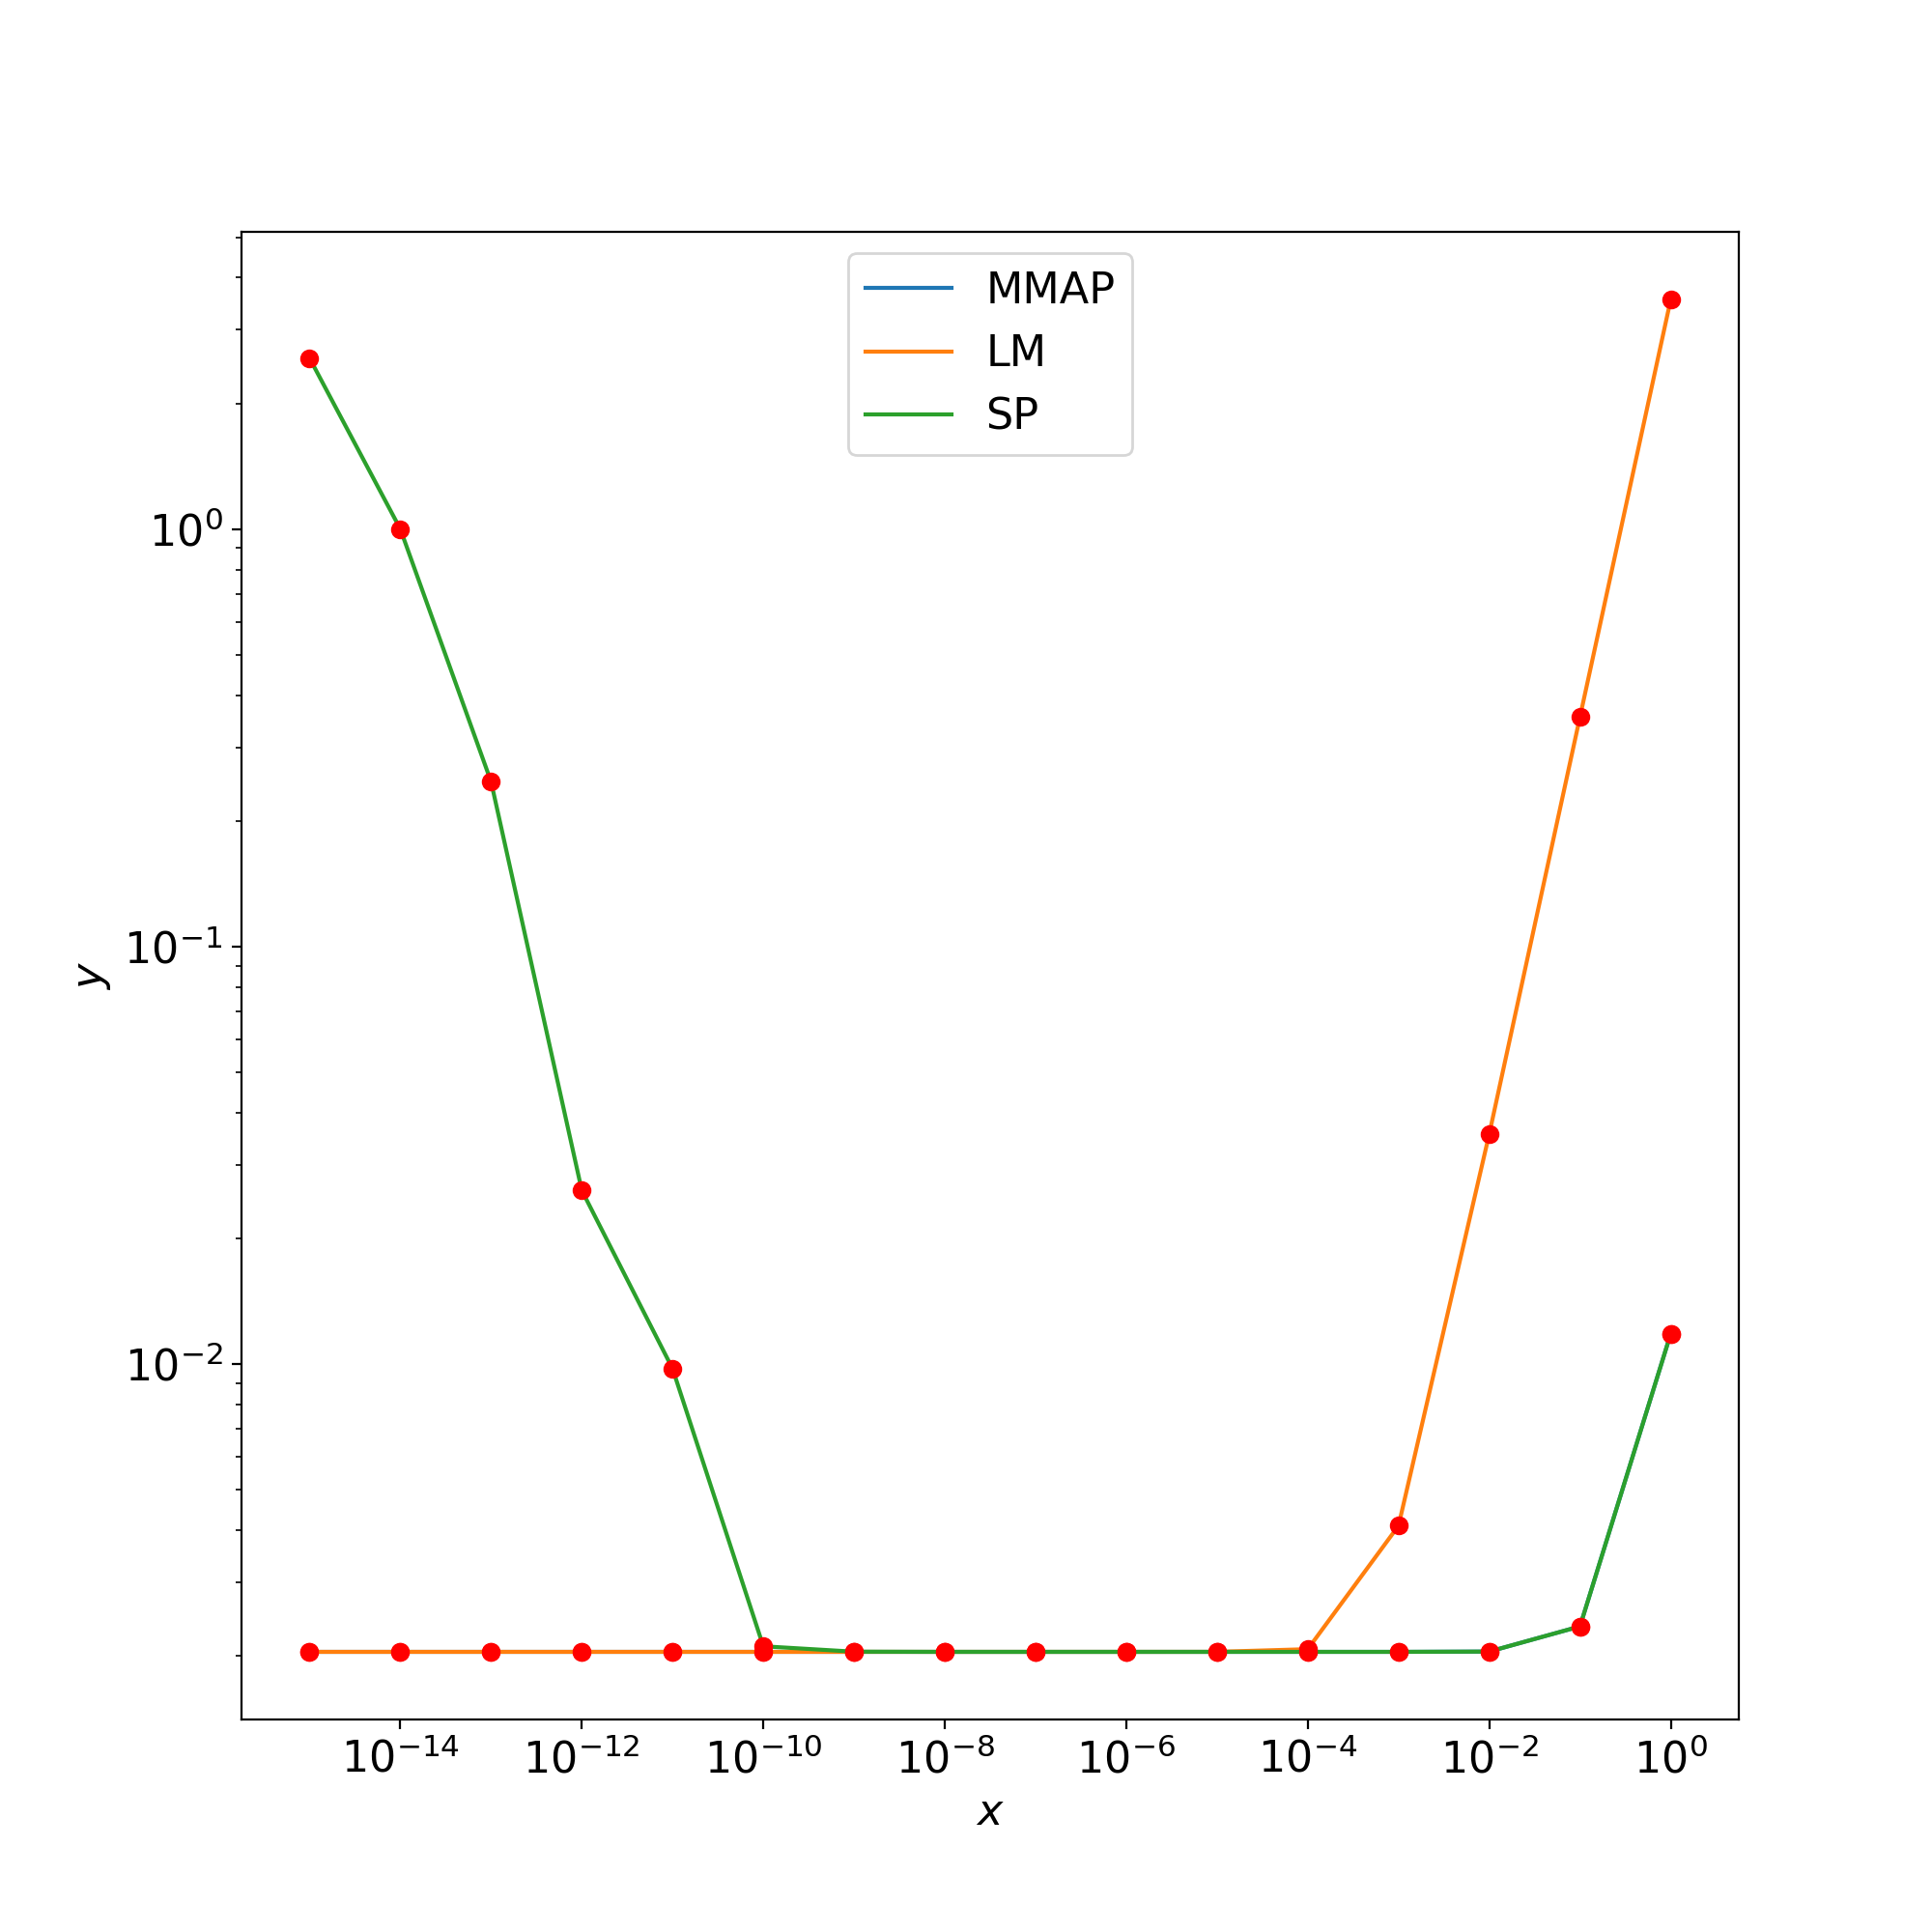
\includegraphics[width=\textwidth]{Pics/LHSims/E1a_MMAP_LM_SPH1.png}
     \caption{H1 Error $\alpha=0$}
 \end{subfigure}
 \begin{subfigure}{0.42\textwidth}
     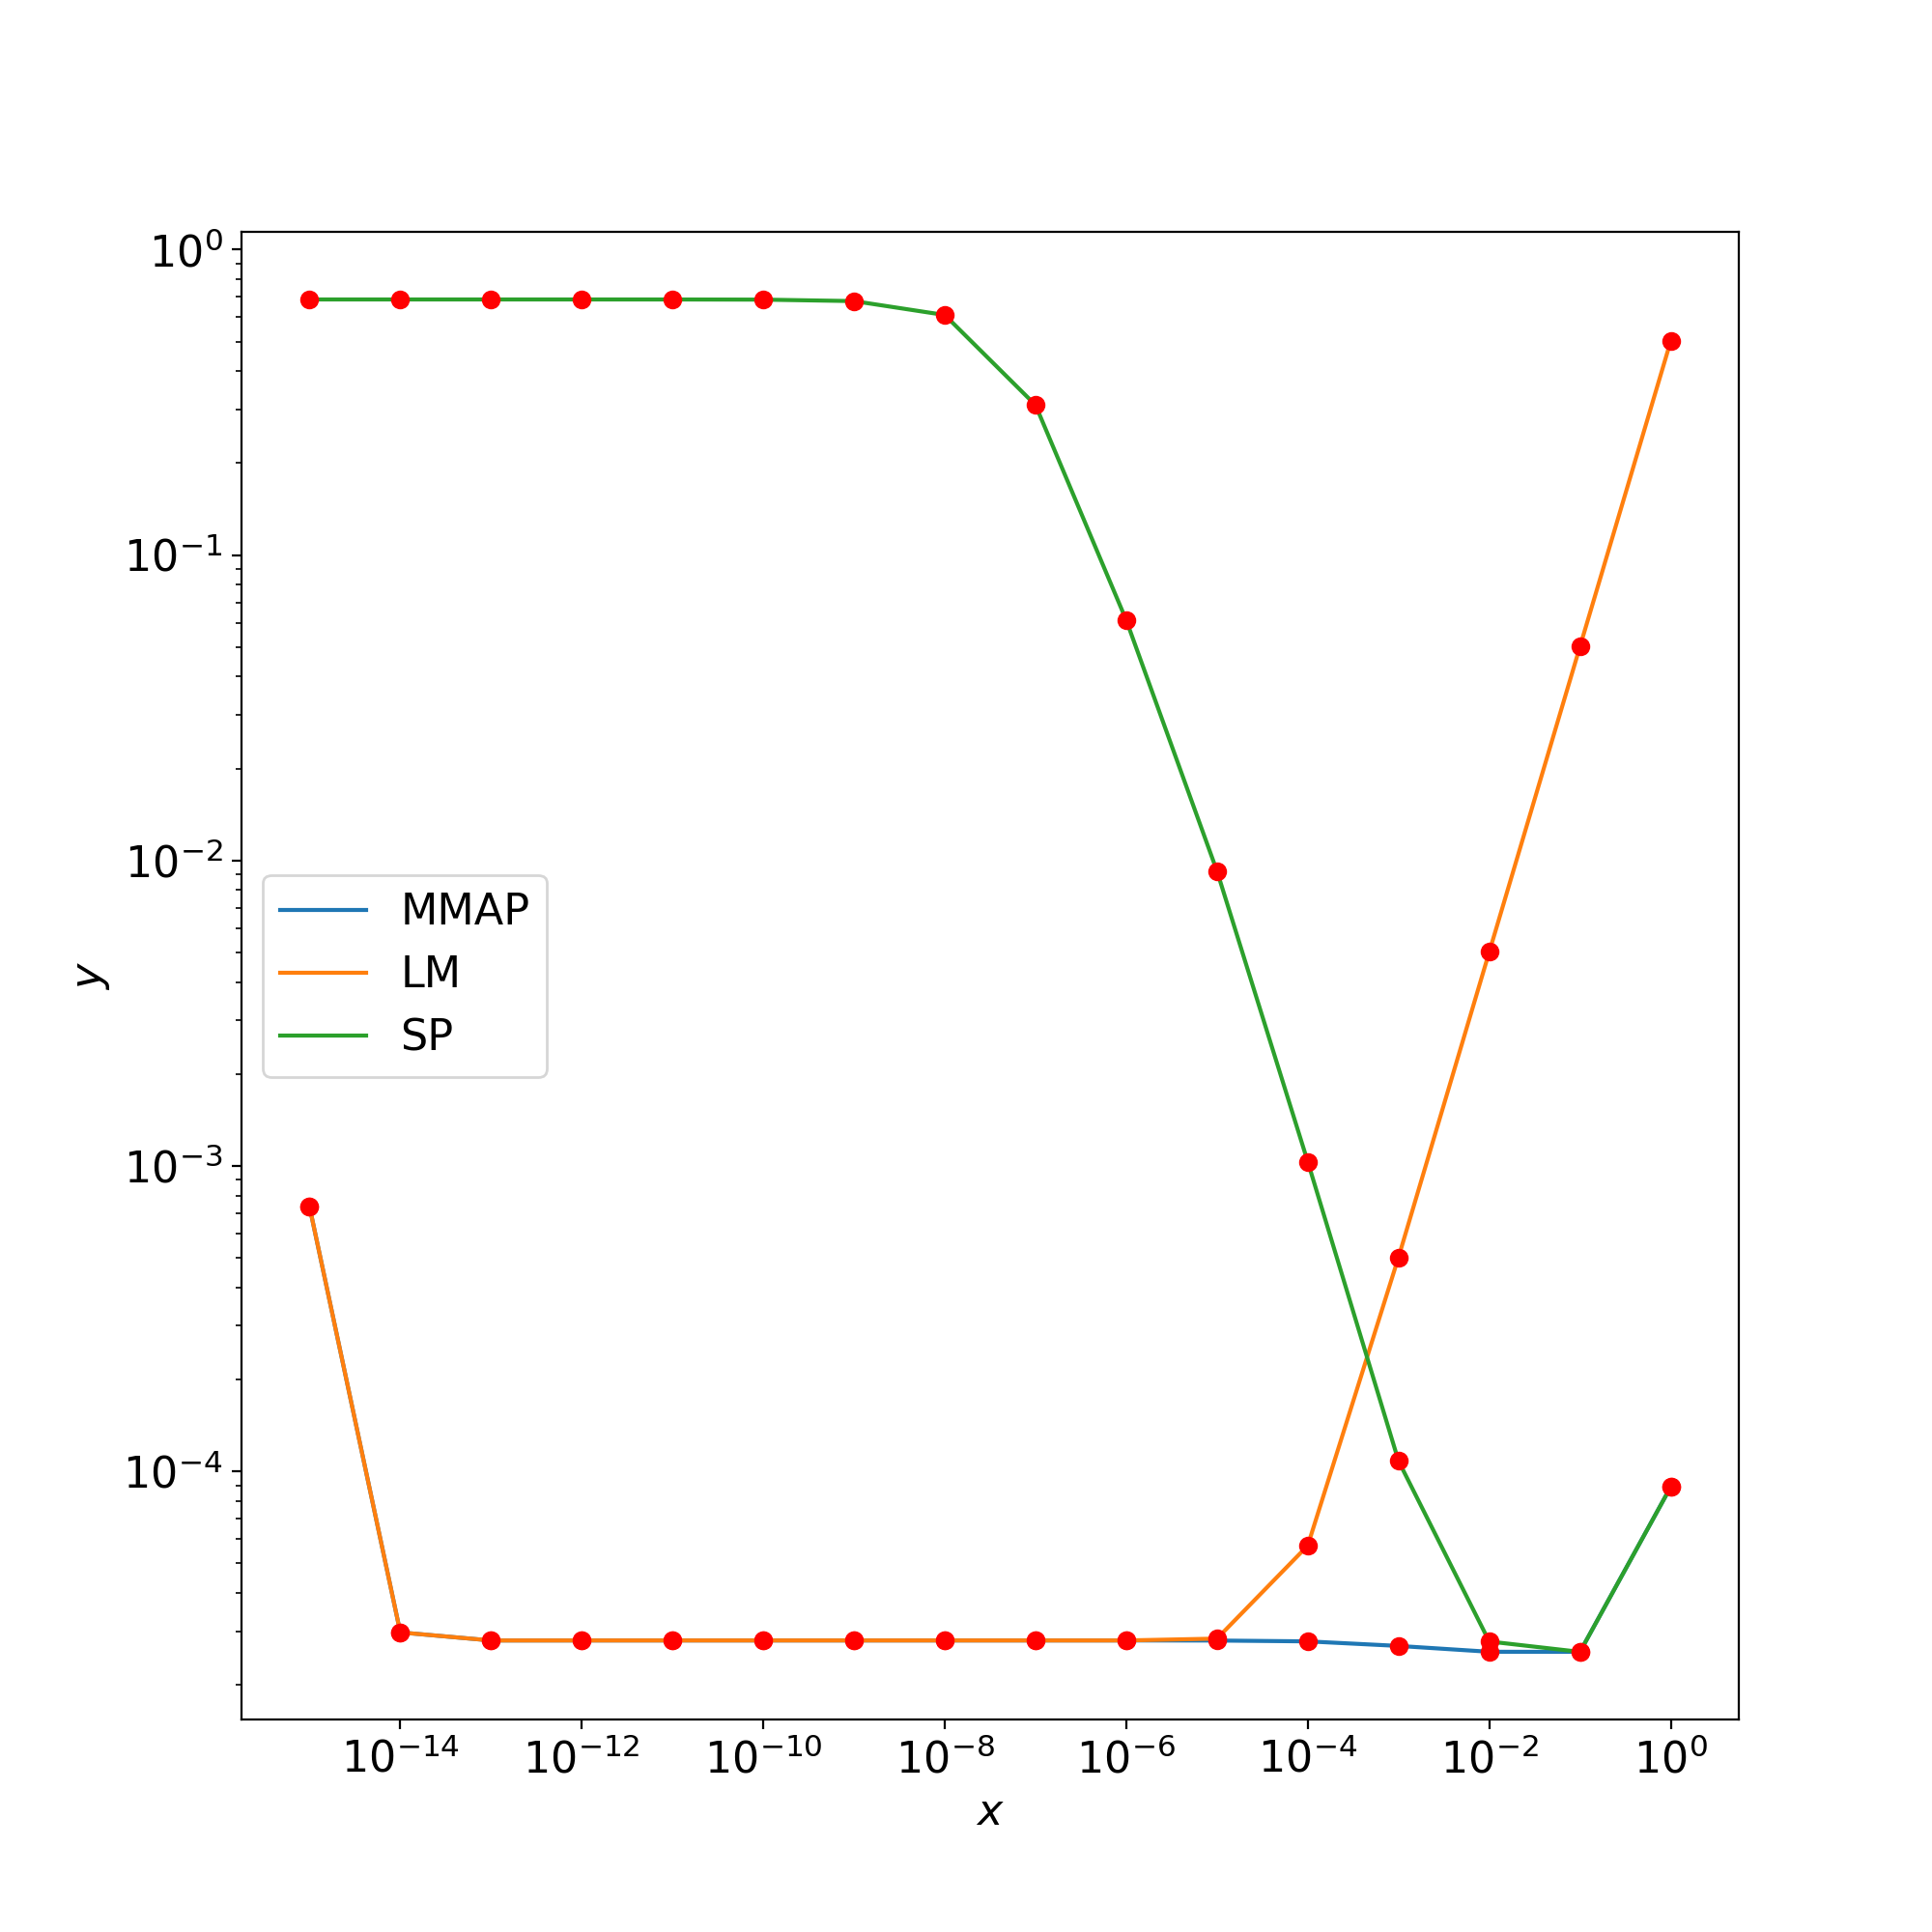
\includegraphics[width=\textwidth]{Pics/LHSims/E1b_MMAP_LM_SPL2.png}
     \caption{L2 Error $\alpha=2, m=1$}
 \end{subfigure}
 \begin{subfigure}{0.42\textwidth}
     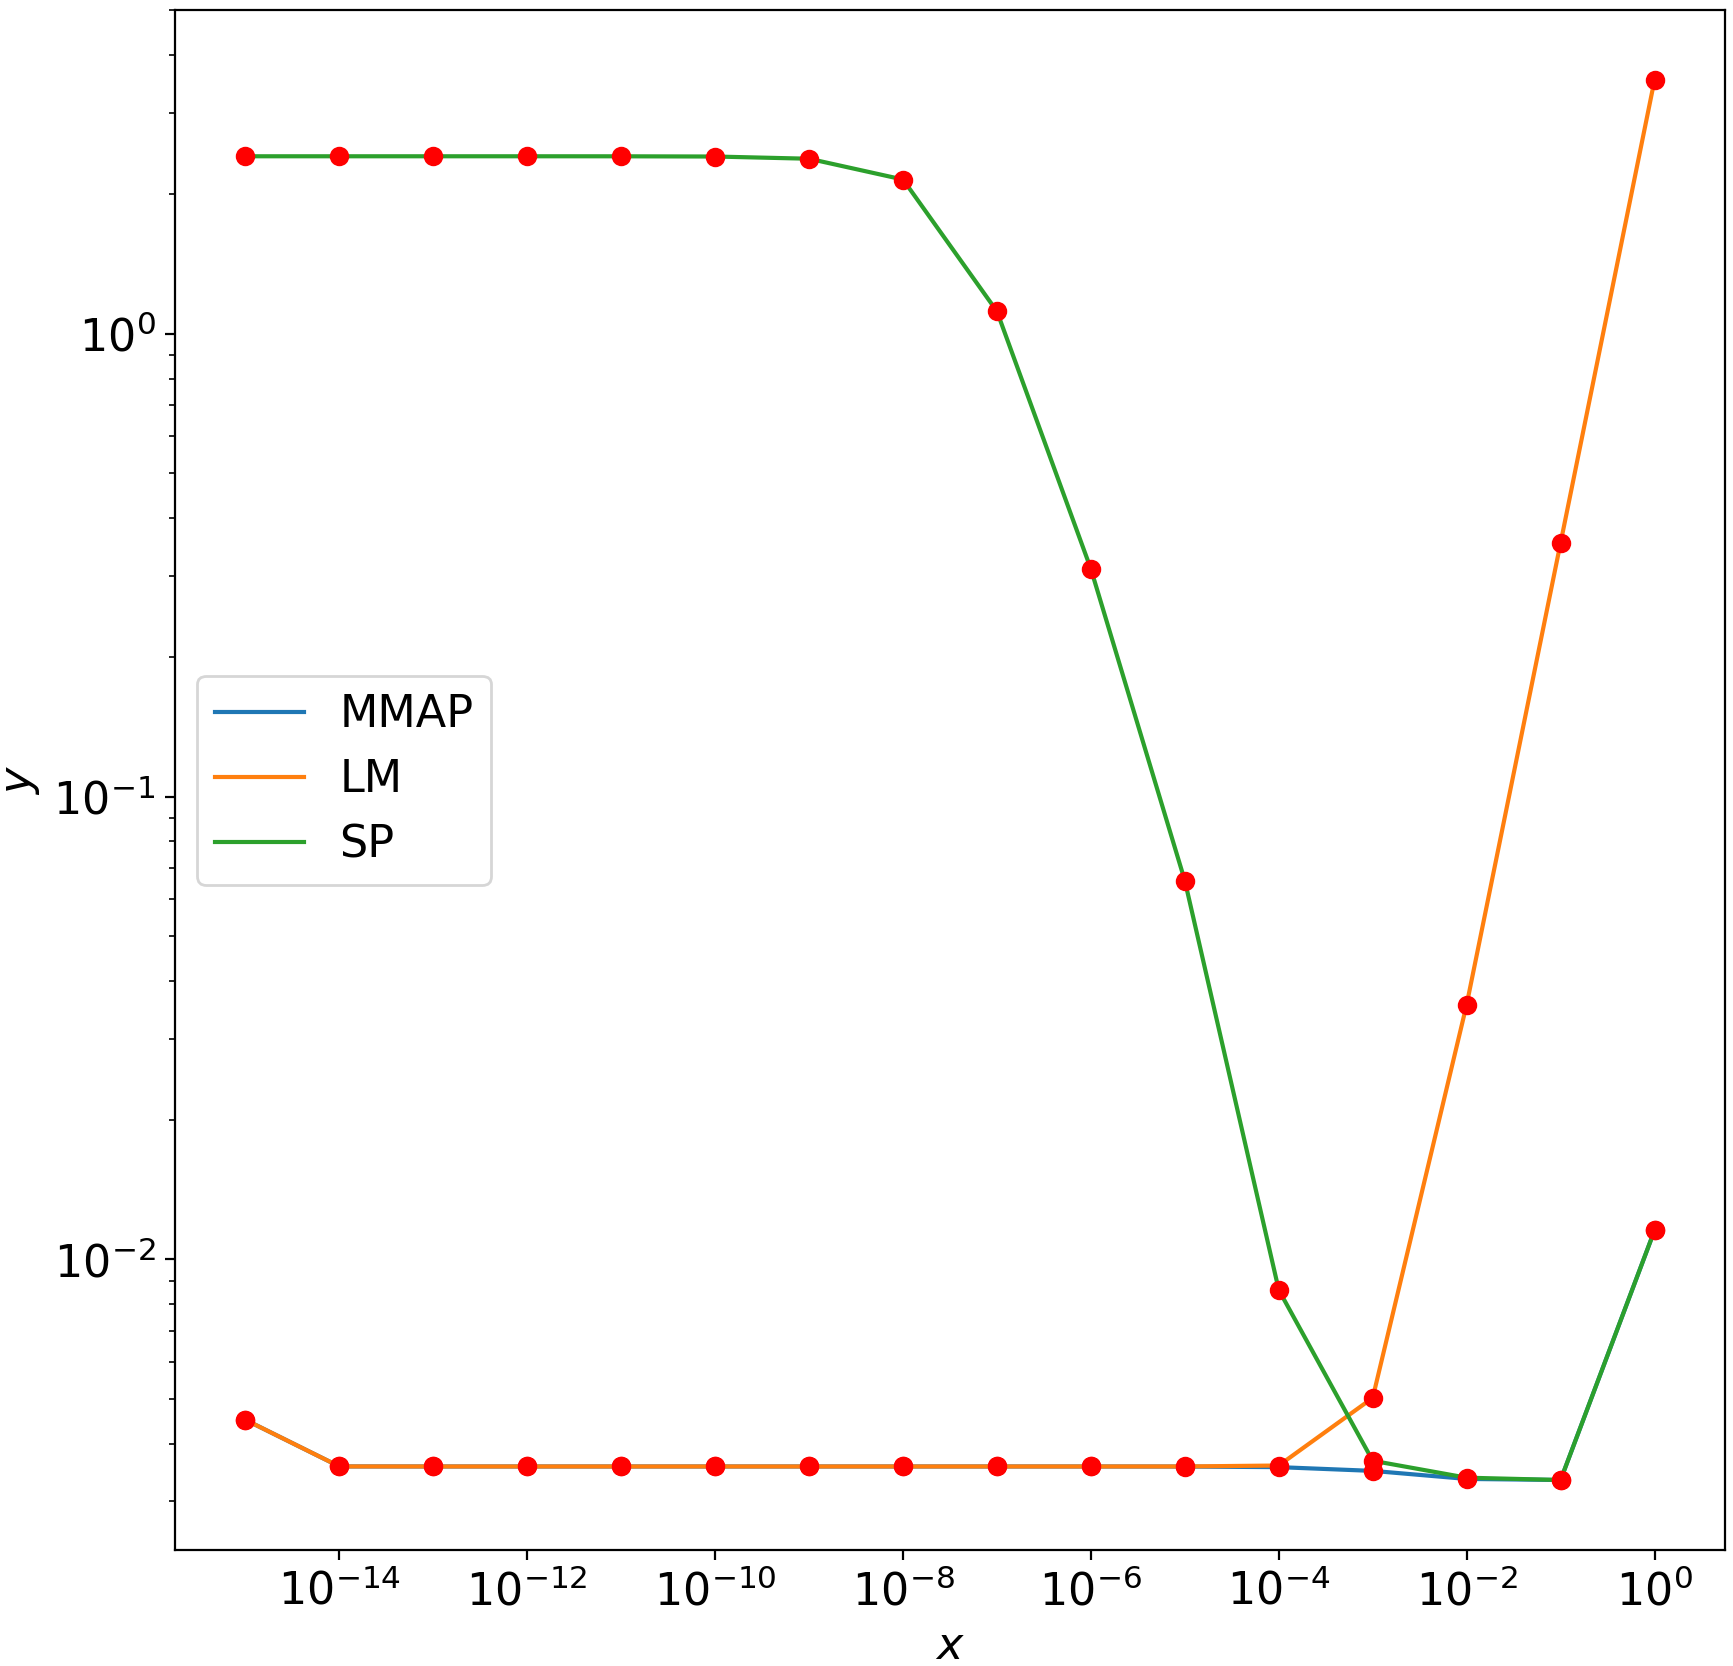
\includegraphics[width=\textwidth]{Pics/LHSims/E1b_MMAP_LM_SPH1.png}
     \caption{H1 Error, $\alpha=2, m=1$}
 \end{subfigure}
 \begin{subfigure}{0.42\textwidth}
     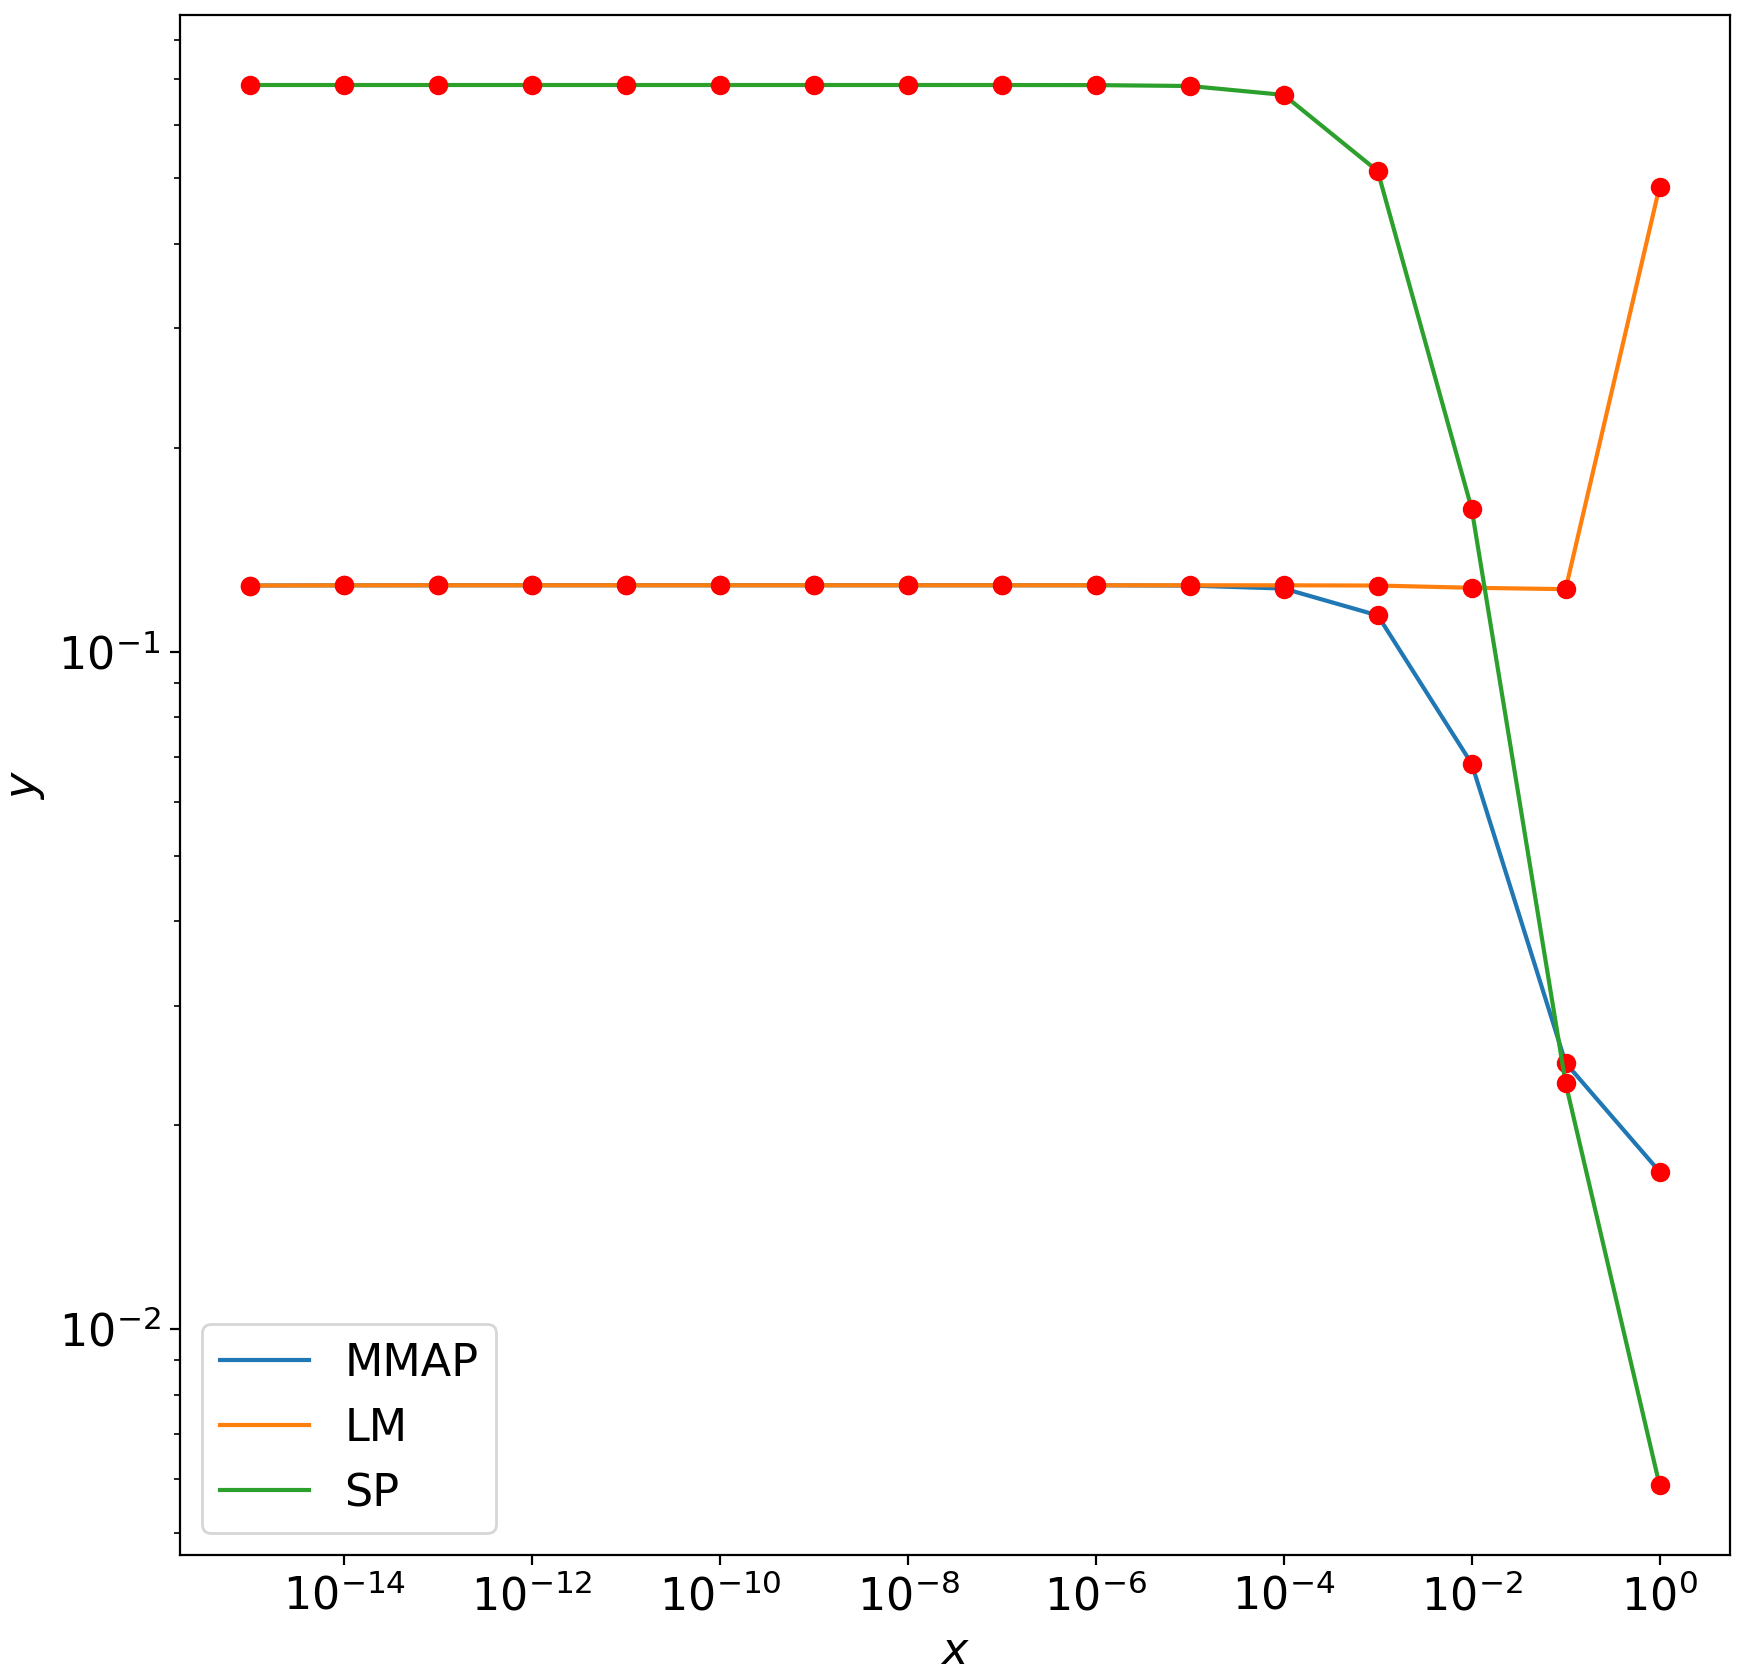
\includegraphics[width=\textwidth]{Pics/LHSims/E1c_MMAP_LM_SPL2.png}
     \caption{L2 Error, $\alpha=2, m=10$}
 \end{subfigure}
 \hfill
 \begin{subfigure}{0.42\textwidth}
     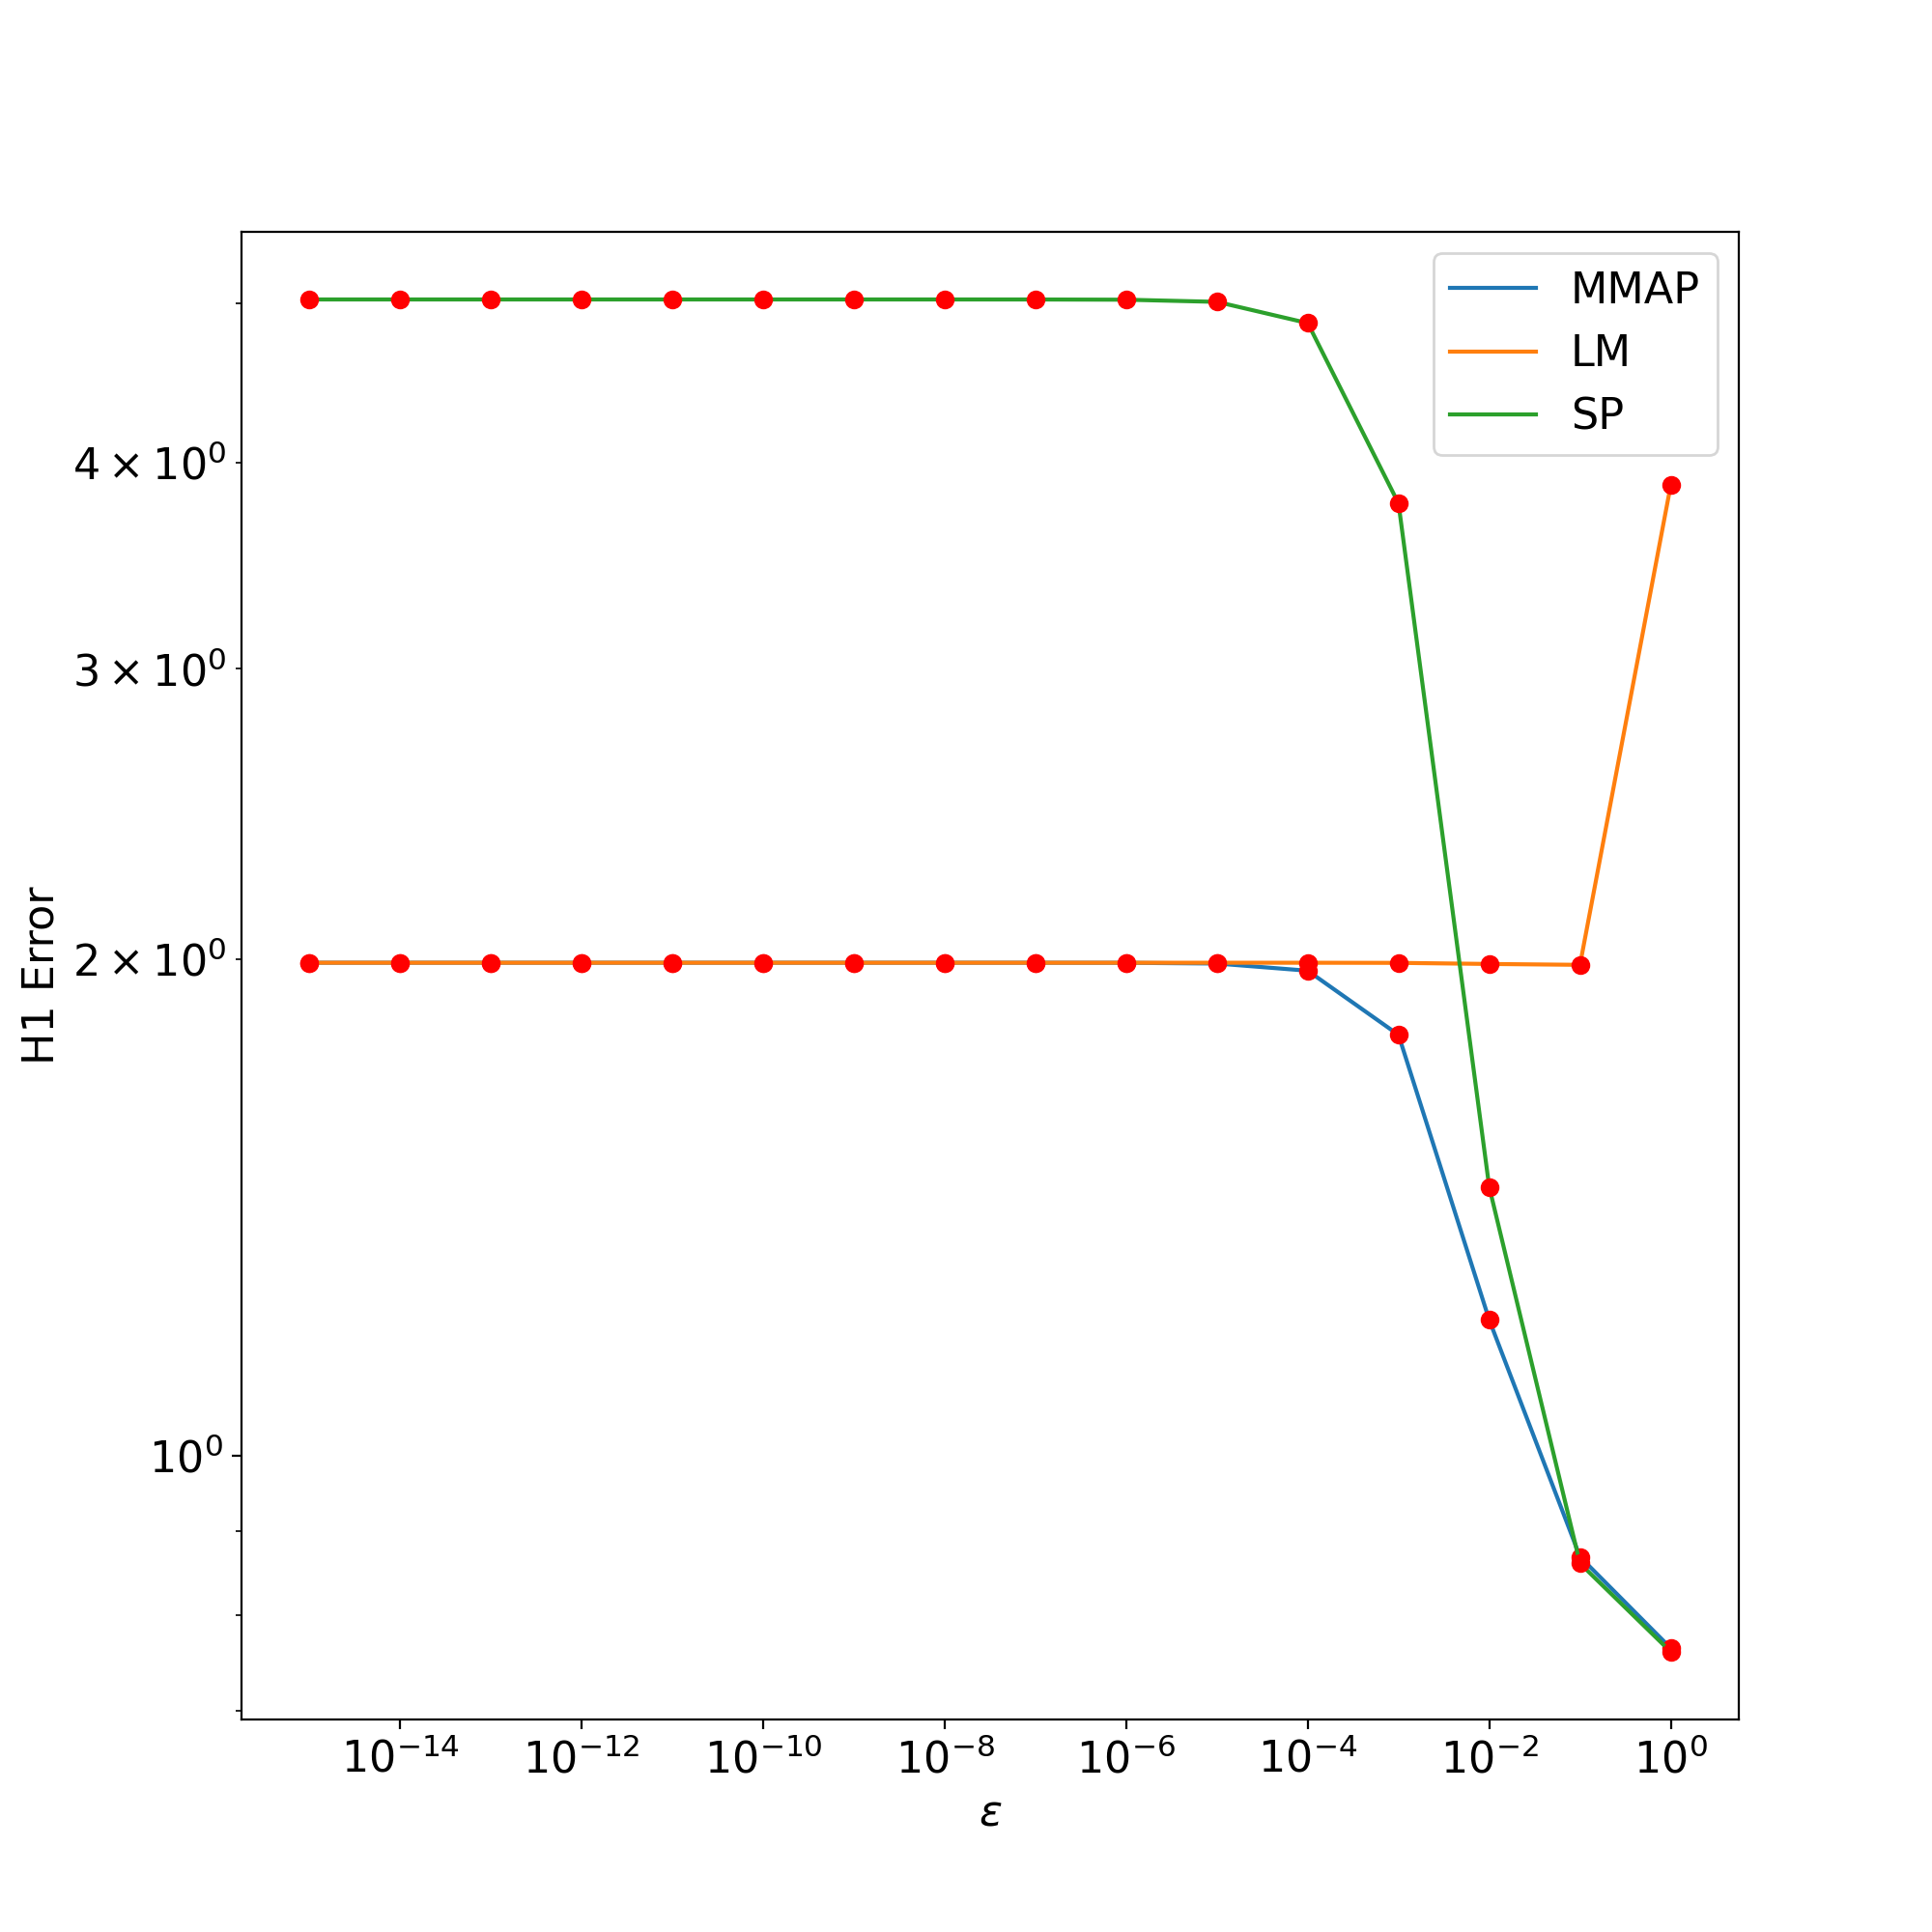
\includegraphics[width=\textwidth]{Pics/LHSims/E1c_MMAP_LM_SPH1.png}
     \caption{H1 Error, $\alpha=2, m=10$}
 \end{subfigure}
 \caption{Numerical demonstration for solver $MMAP, LM$ and $SP$ on a $20\times 20$ quadrilateral grid using CG order $2$ for Example $1$, with $x=\varepsilon$ and $y=$ Error.} \label{E1_LM_SP}
\end{figure}






\begin{table}[]
\resizebox{\textwidth}{!}{
\begin{tabular}{||ccccc||}
\cline{2-5}
\multicolumn{1}{c|}{} & \multicolumn{2}{c|}{$\Gamma_{in} := \{x=0\}$} & \multicolumn{2}{c|}{$\Gamma_{in} := \{x=1\}$}\\
\hline 
L2 Error & PF        & MMAP        & PF        & MMAP   \\
\hline \hline
$\alpha = 0$ & $2.4624E-07$  & $2.4624E-07$ & $2.4624E-07$ & $2.4624E-07$\\
\hline
$\alpha = 2, m=1$ & 
$2.3834E-05$  & $4.2451E-07$ & $2.3834E-05$ & $4.2451E-07$\\
\hline
$\alpha = 2, m=10$ & 
$9.7179E-04$  & $9.7017E-04$ & $9.7179E-04$ & $9.7017E-04$\\
\hline
\end{tabular}}
\end{table}

\begin{table}[]
\resizebox{\textwidth}{!}{
\begin{tabular}{||ccccc||}
\cline{2-5}
\multicolumn{1}{c|}{} & \multicolumn{2}{c|}{$\Gamma_{in} := \{x=0\}$} & \multicolumn{2}{c|}{$\Gamma_{in} := \{x=1\}$}\\
\hline 
H1 Error & PF        & MMAP        & PF        & MMAP   \\
\hline \hline
$\alpha = 0$ &
$1.2767E-04$  & $1.2767E-04$ & $1.2767E-04$ & $1.2767E-04$\\
\hline
$\alpha = 2, m=1$ & 
$7.2261E-03$  & $2.2108E-04$ & $7.2261E-03$ & $2.2108E-04$\\
\hline
$\alpha = 2, m=10$ &
$2.0097E-01$  & $4.9986E-02$ & $2.0097E-01$ & $4.9986E-02$\\
\hline
\end{tabular}}
\caption{Error for different definitions of $\Gamma_{in}$ on an $80 \times 80$ quadrilateral grid with order $2$ Lagrange finite element, $51842$ degrees of freedom and $\varepsilon=10^{-10}$.}
\label{tbl_E1_diff_Gam}
\end{table}

Thus numerical experimentation shown in Table \ref{tbl_E1_diff_Gam} strongly suggests that the set $\mathcal{L}$ can be set to zero anywhere on the streamline. In other words, if $\Gamma_{SL} := \{\text{ one point on every streamline }\}$ then we can have $\mathcal{L} := \{\lambda \in \mathcal{H}^1(\Omega): \lambda|_{\Gamma_{SL}\cup \Gamma_{D}}=0\}$.

\section{Example 2, Annulus}
We now propose an example of an annulus with closed field lines.
We will solve the PDE (\ref{PDE}) with $\Omega := \{x,y \in \mathbb{R}, 1<x^2+y^2<4\}$, $\Gamma_D := \{x,y \in \mathbb{R}, (x^2+y^2=1 \text{ or } x^2+y^2=4)\}$ and $\Gamma_N := \emptyset$. We chose the magnetic field 
\begin{equation}
\mathbf{b} = \frac{\mathbf{B}}{|\mathbf{B}|} = 
\left[ \begin{matrix}
-y\\
 x
\end{matrix} \right]/\sqrt{x^2+y^2}, 
\mathbf{B} = \left[ \begin{matrix}
-y\\
 x
\end{matrix} \right]
\end{equation}
which is visualised in Figure \ref{E2_VF} and the streamlines follow the equation
\begin{equation}
x^2 + y^2 = R^2, \text{ with } 1\leq R \leq 2.
\end{equation}
\begin{figure}[H]
 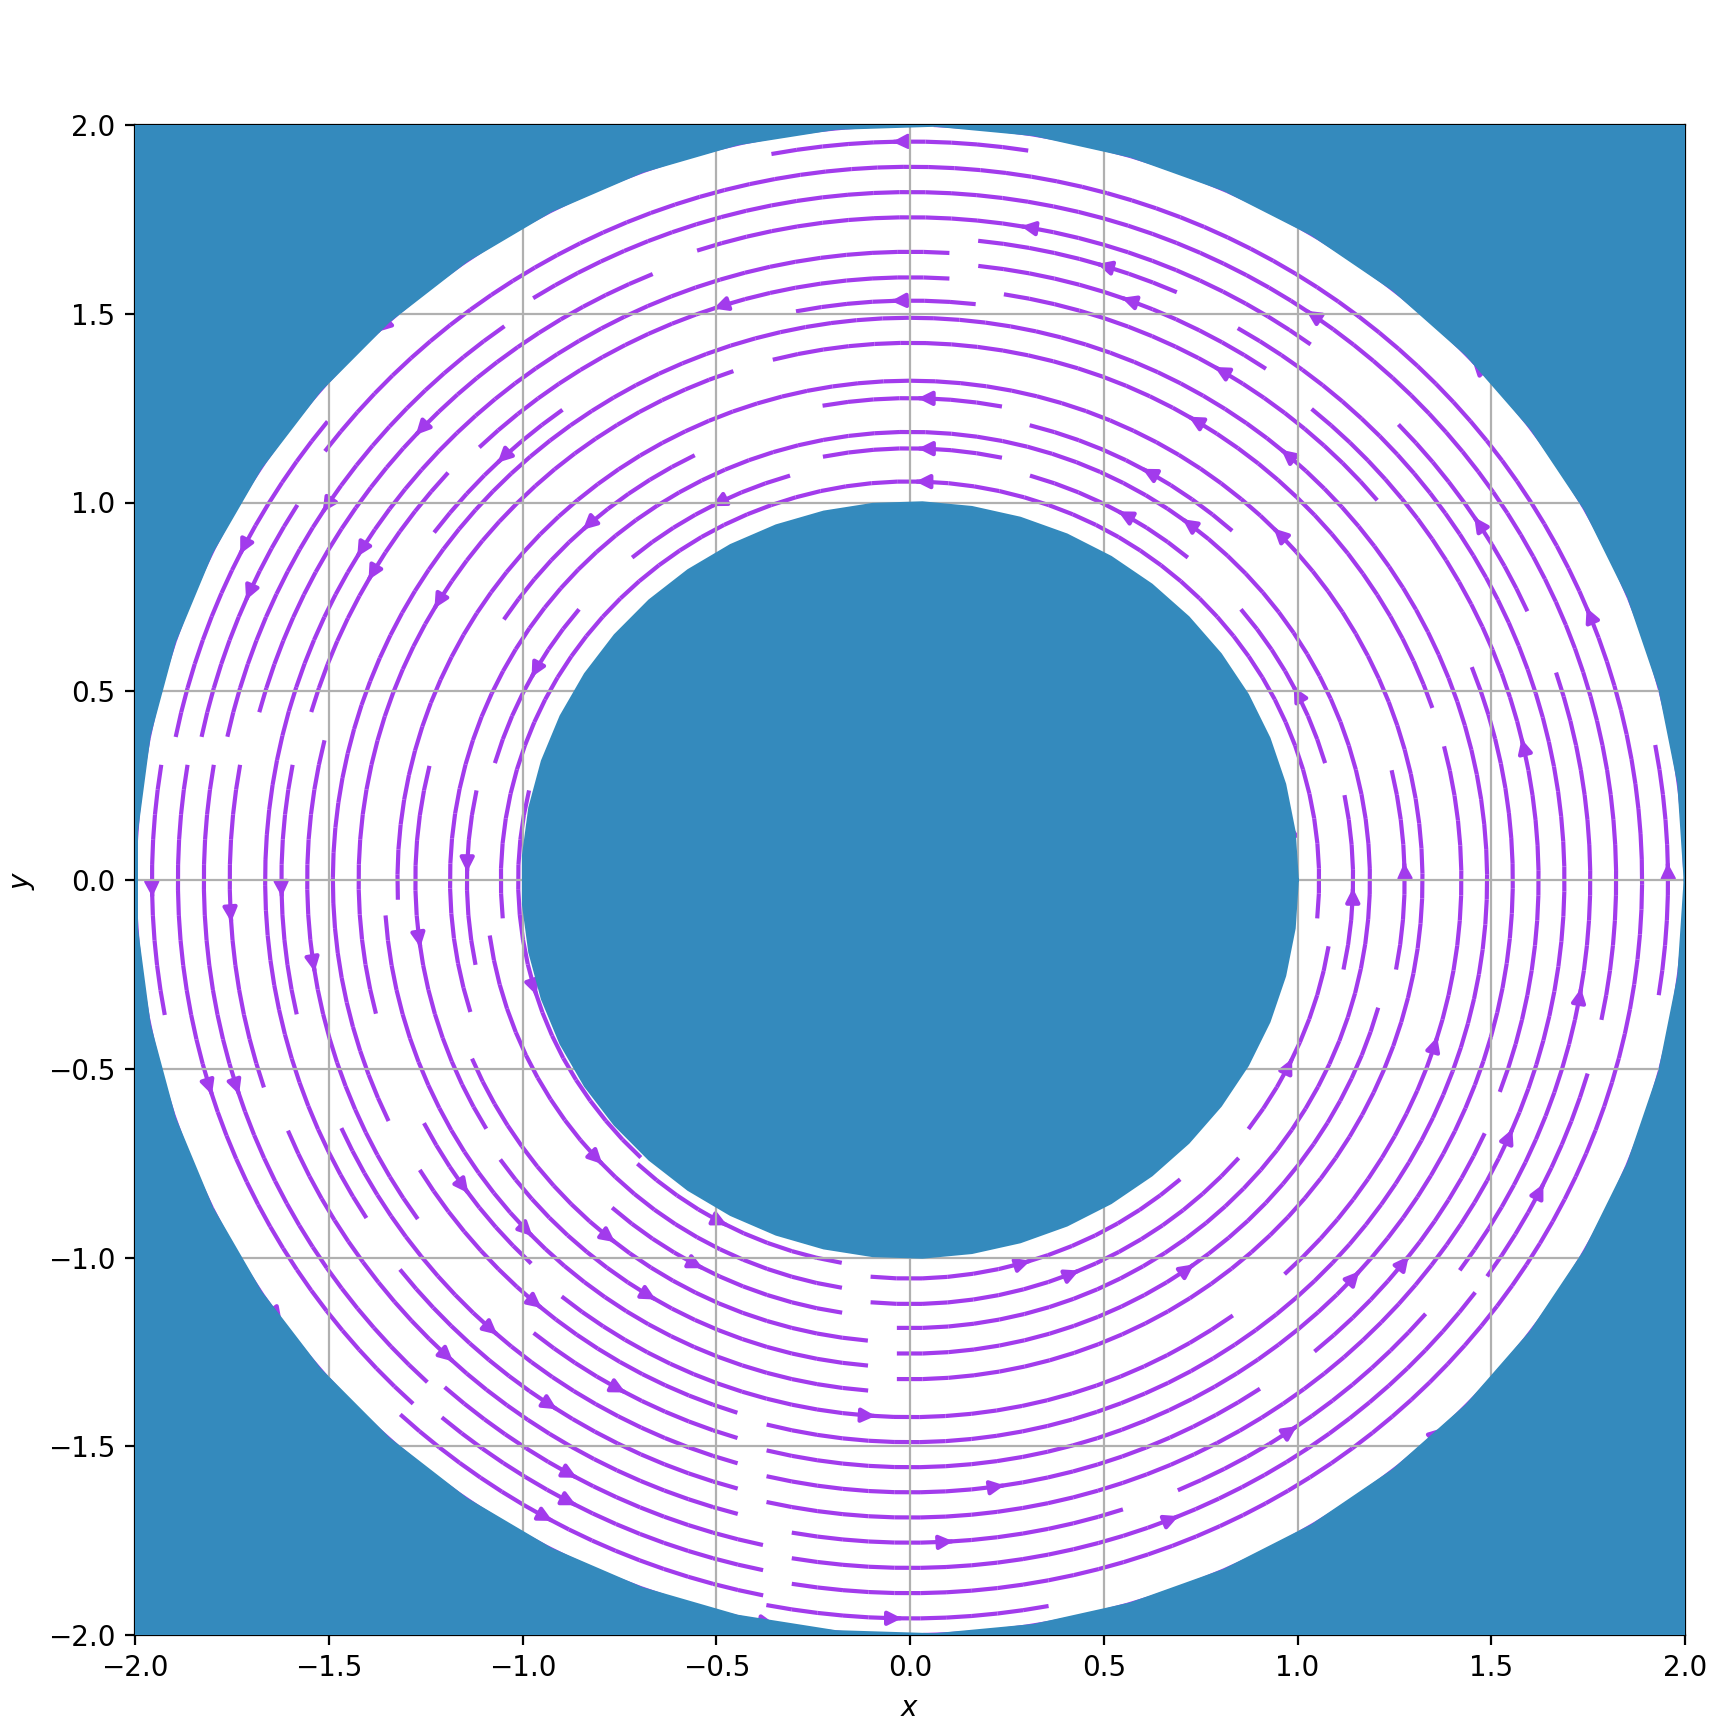
\includegraphics[width=\textwidth]{Pics/VectorField/E2b.png}
  \caption{Electromagnetic field $\mathbf{b}$ for Example $2$.}
 \label{E2_VF}
\end{figure}

From Fig \ref{E2_VF} it can be seen the magnetic field has closed lines. Therefore, for methods which involve $\Gamma_{in}$ we use the stabilisation variants. However, from the numerical investigation of Example 1 from Table \ref{tbl_E1_diff_Gam} we found that we can change $\Gamma_{in}$ to $\Gamma_{out}$ and get a similar error. This strongly suggests that $\Gamma_{in}$ can represent a point on each streamline. Thus we will numerically investigate the consequence of setting $\Gamma_{in}:=\{x,y \in \mathbb{R}, x>0, y=0\}$.

We will use the solution
\begin{equation}
u = (1+\varepsilon)(x^2 + y^2 -1)(4-x^2-y^2)
\end{equation}
which is visualised with its source term $f$ in Figure \ref{E2_uf} at $\varepsilon = 0.1$.
\begin{figure}[H]
 \begin{subfigure}{0.5\textwidth}
     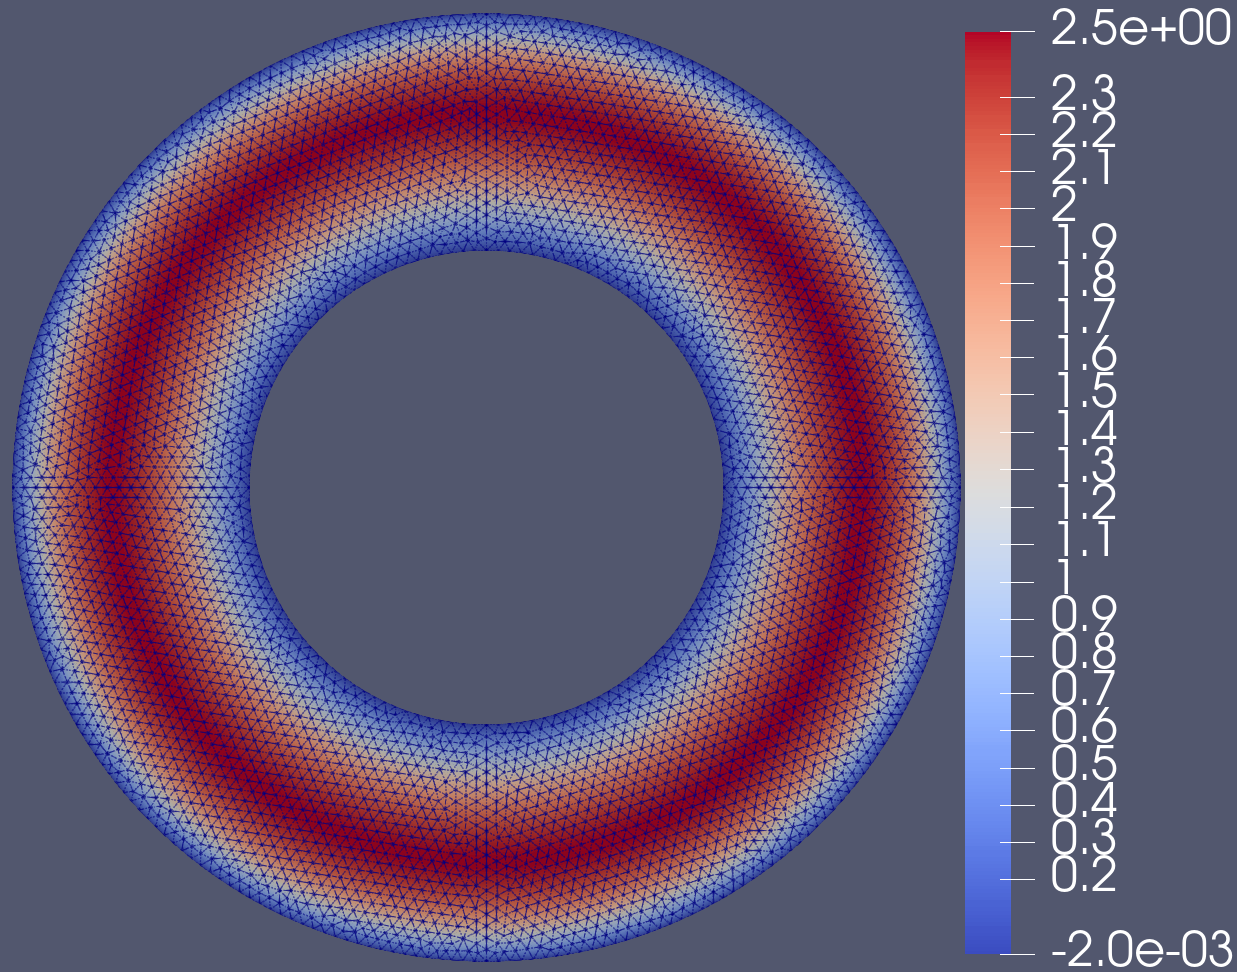
\includegraphics[width=\textwidth]{Pics/uf/U_E2_eps_1.png}
     \caption{Exact solution $u$ with mesh.}
 \end{subfigure}
   \begin{subfigure}{0.5\textwidth}
     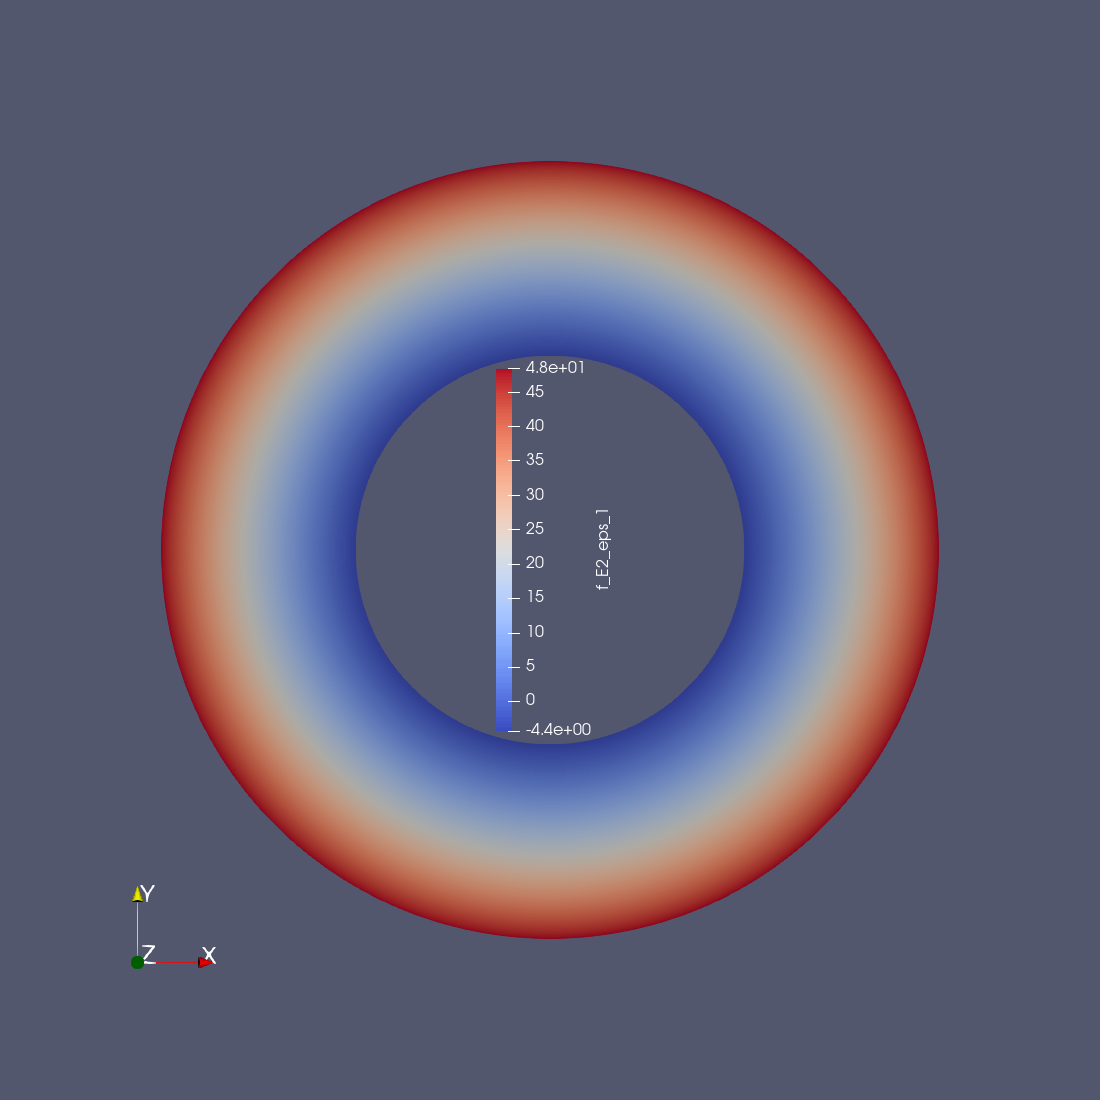
\includegraphics[width=\textwidth]{Pics/uf/F_E2_eps_1.png}
     \caption{Source term $f$.}
 \end{subfigure}
 \caption{Example $2$ with $\varepsilon = 0.1$} \label{E2_uf}
\end{figure}

In Figure \ref{E2_LH} we have numerical calculations for varying $\varepsilon$ for Example $2$ with degrees $36944$ of freedom. As can be seen by Figures \ref{E2_LH_L2} and \ref{E2_LH_H1} when there are closed field lines the methods $(PF)$ and $(MMAP)$ fail to produce accurate solutions for $\varepsilon \ll 1$.

However, in Figures \ref{E2_LH_L2_CON} and \ref{E2_LH_H1_CON} we change $\Gamma_{in} := \emptyset$ to $\Gamma_{in}:=\{x,y \in \mathbb{R}, x>0, y=0\}$. This change makes a negligible difference to the $(PF)$ method. It is currently unclear why there is no difference, the code has been checked multiple times but no error has been found. But, the change leads to a significant improvement for the $(MMAP)$. Therefore, we propose a new variant of the $(MMAP)$ where the definition of the set $\mathcal{L}$ is $\{\lambda \in \mathcal{H}^1(\Omega): \lambda|_{\Gamma_{CL}\cup \Gamma_{D}}=0\}$.

The new $(MMAP)$ variant is not discussed further because Figures \ref{E2_LH_L2_STAB} and \ref{E2_LH_H1_STAB} show methods $(MMAP\_STAB)$ and $(PF\_STAB)$ outperform the $(MMAP)$ variant. Thus for the following examples, we only consider methods $(MMAP\_STAB)$ and $(PF\_STAB)$.

\begin{figure}[H]
 \begin{subfigure}{0.42\textwidth}
     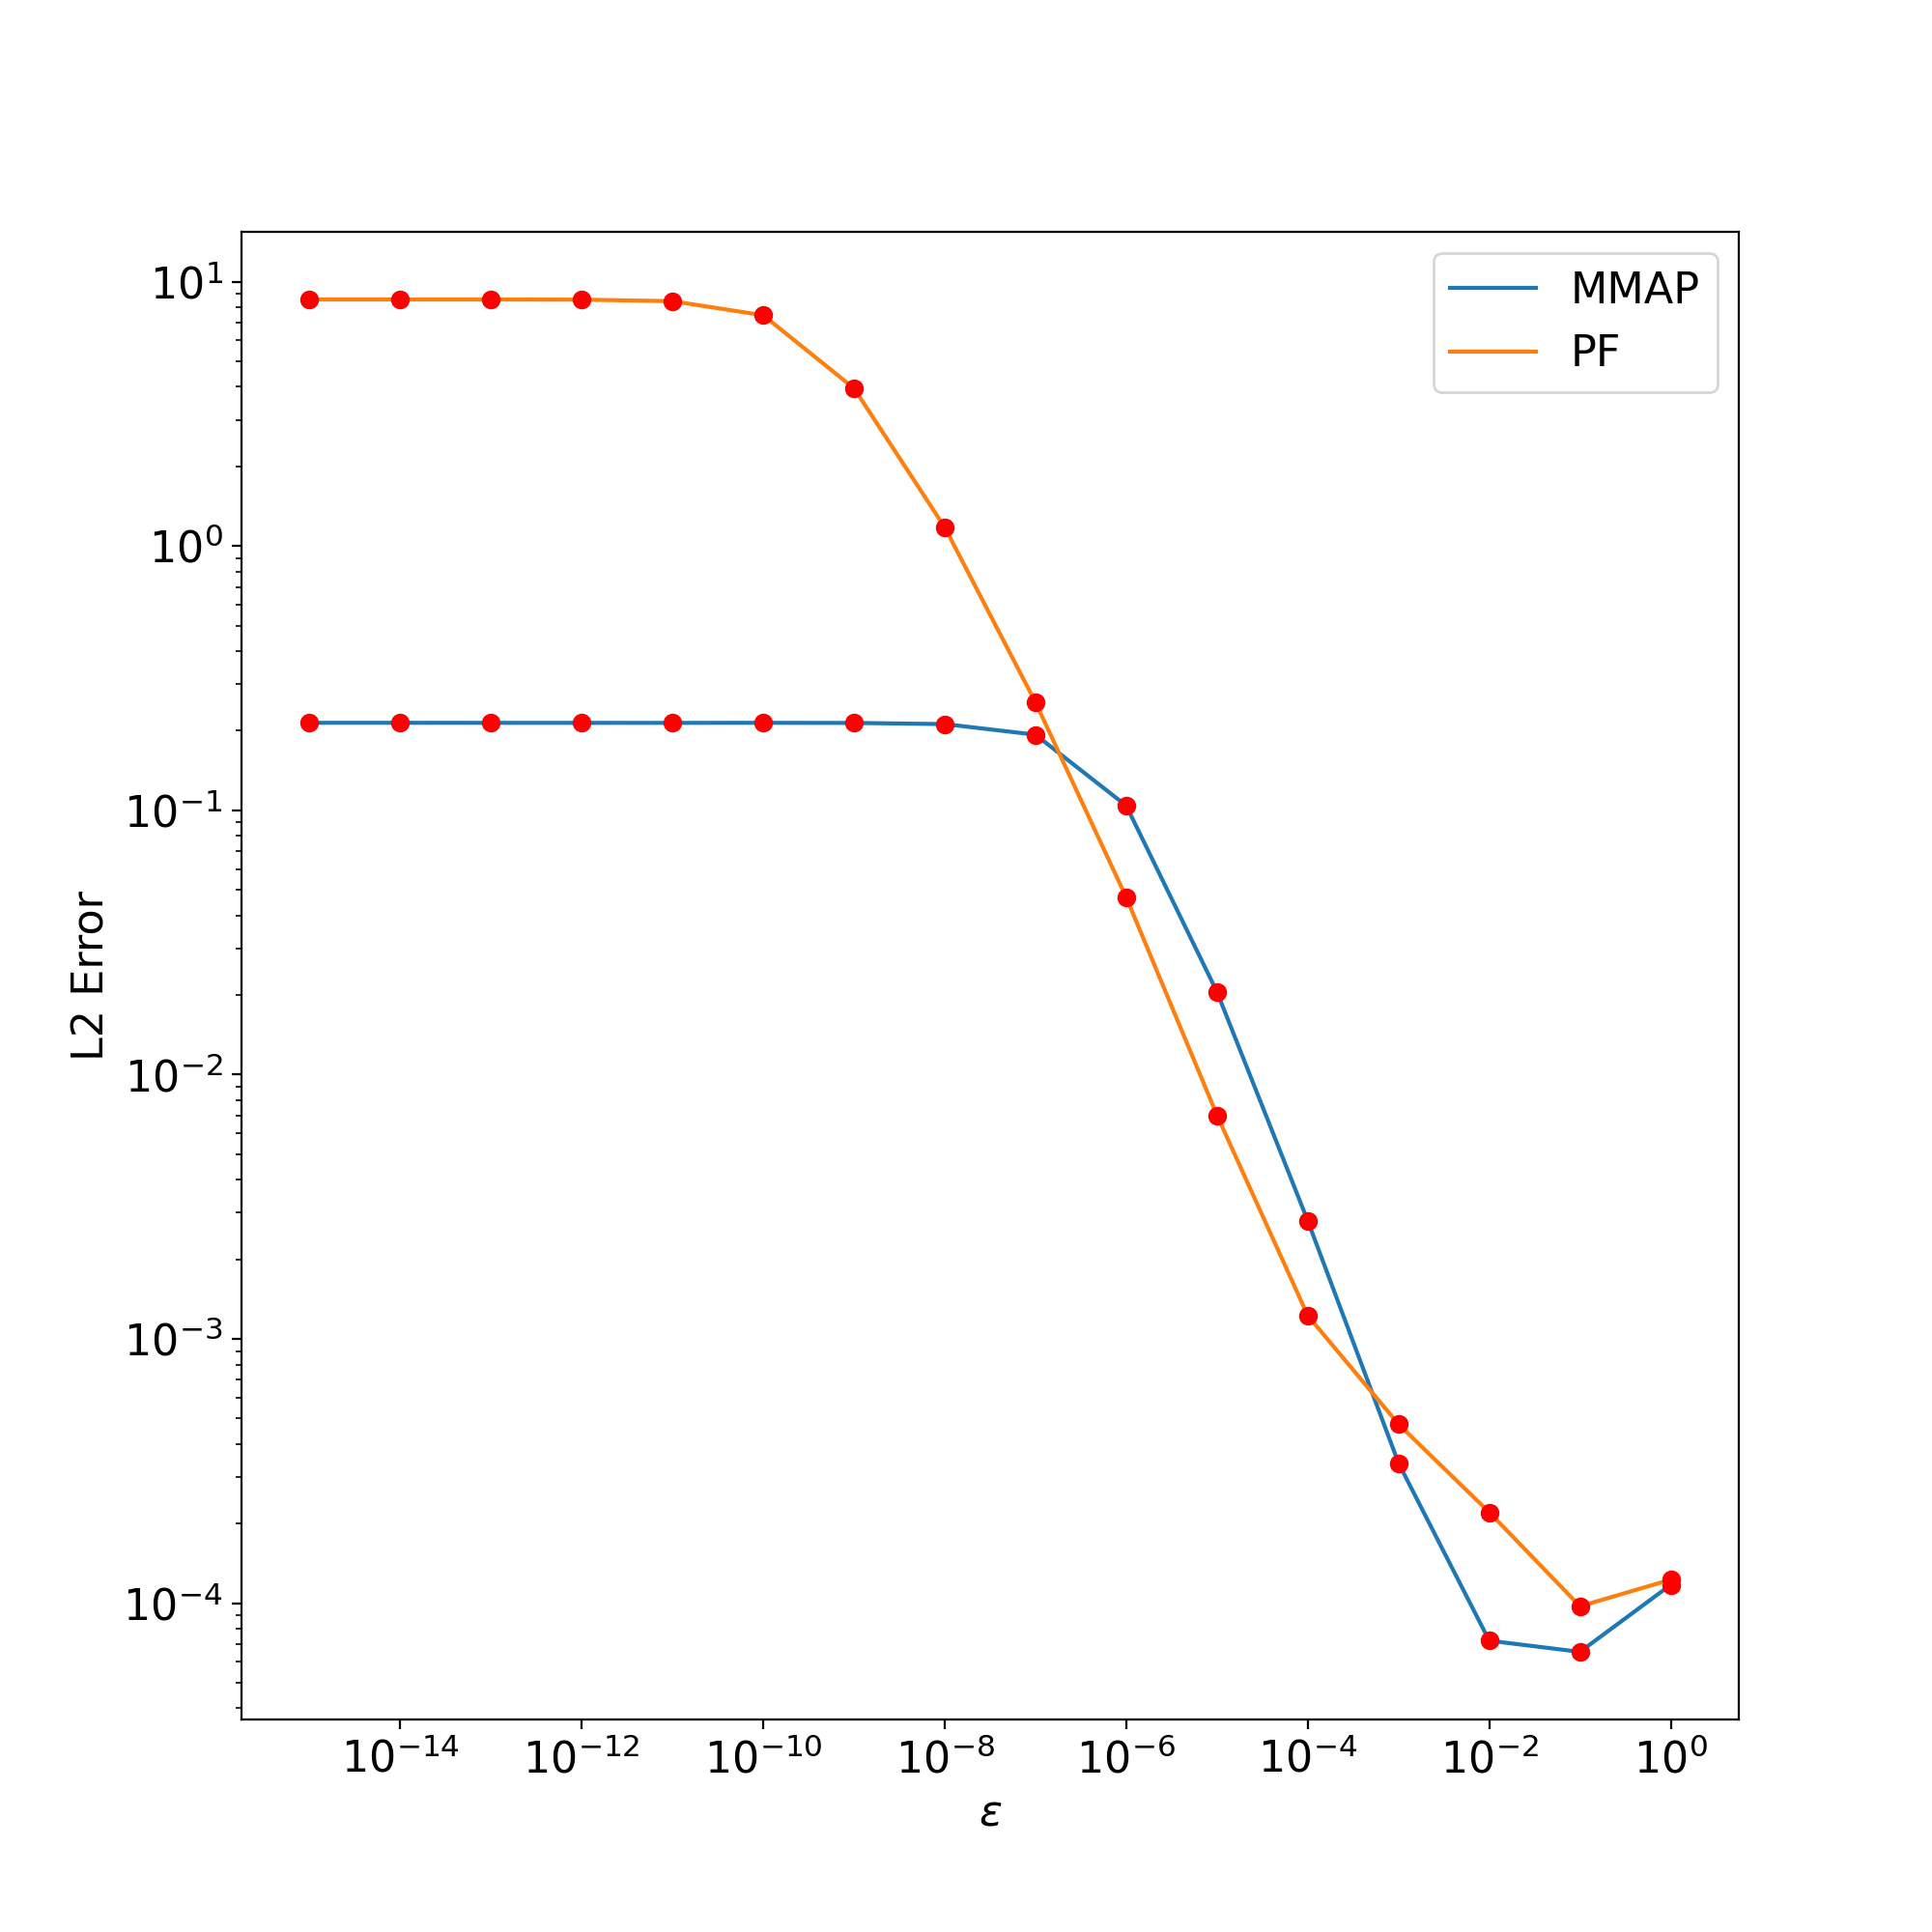
\includegraphics[width=\textwidth]{Pics/LHSims/E2/E2_NormalL2.png}
     \caption{L2 Error} \label{E2_LH_L2}
 \end{subfigure}
   \begin{subfigure}{0.42\textwidth}
     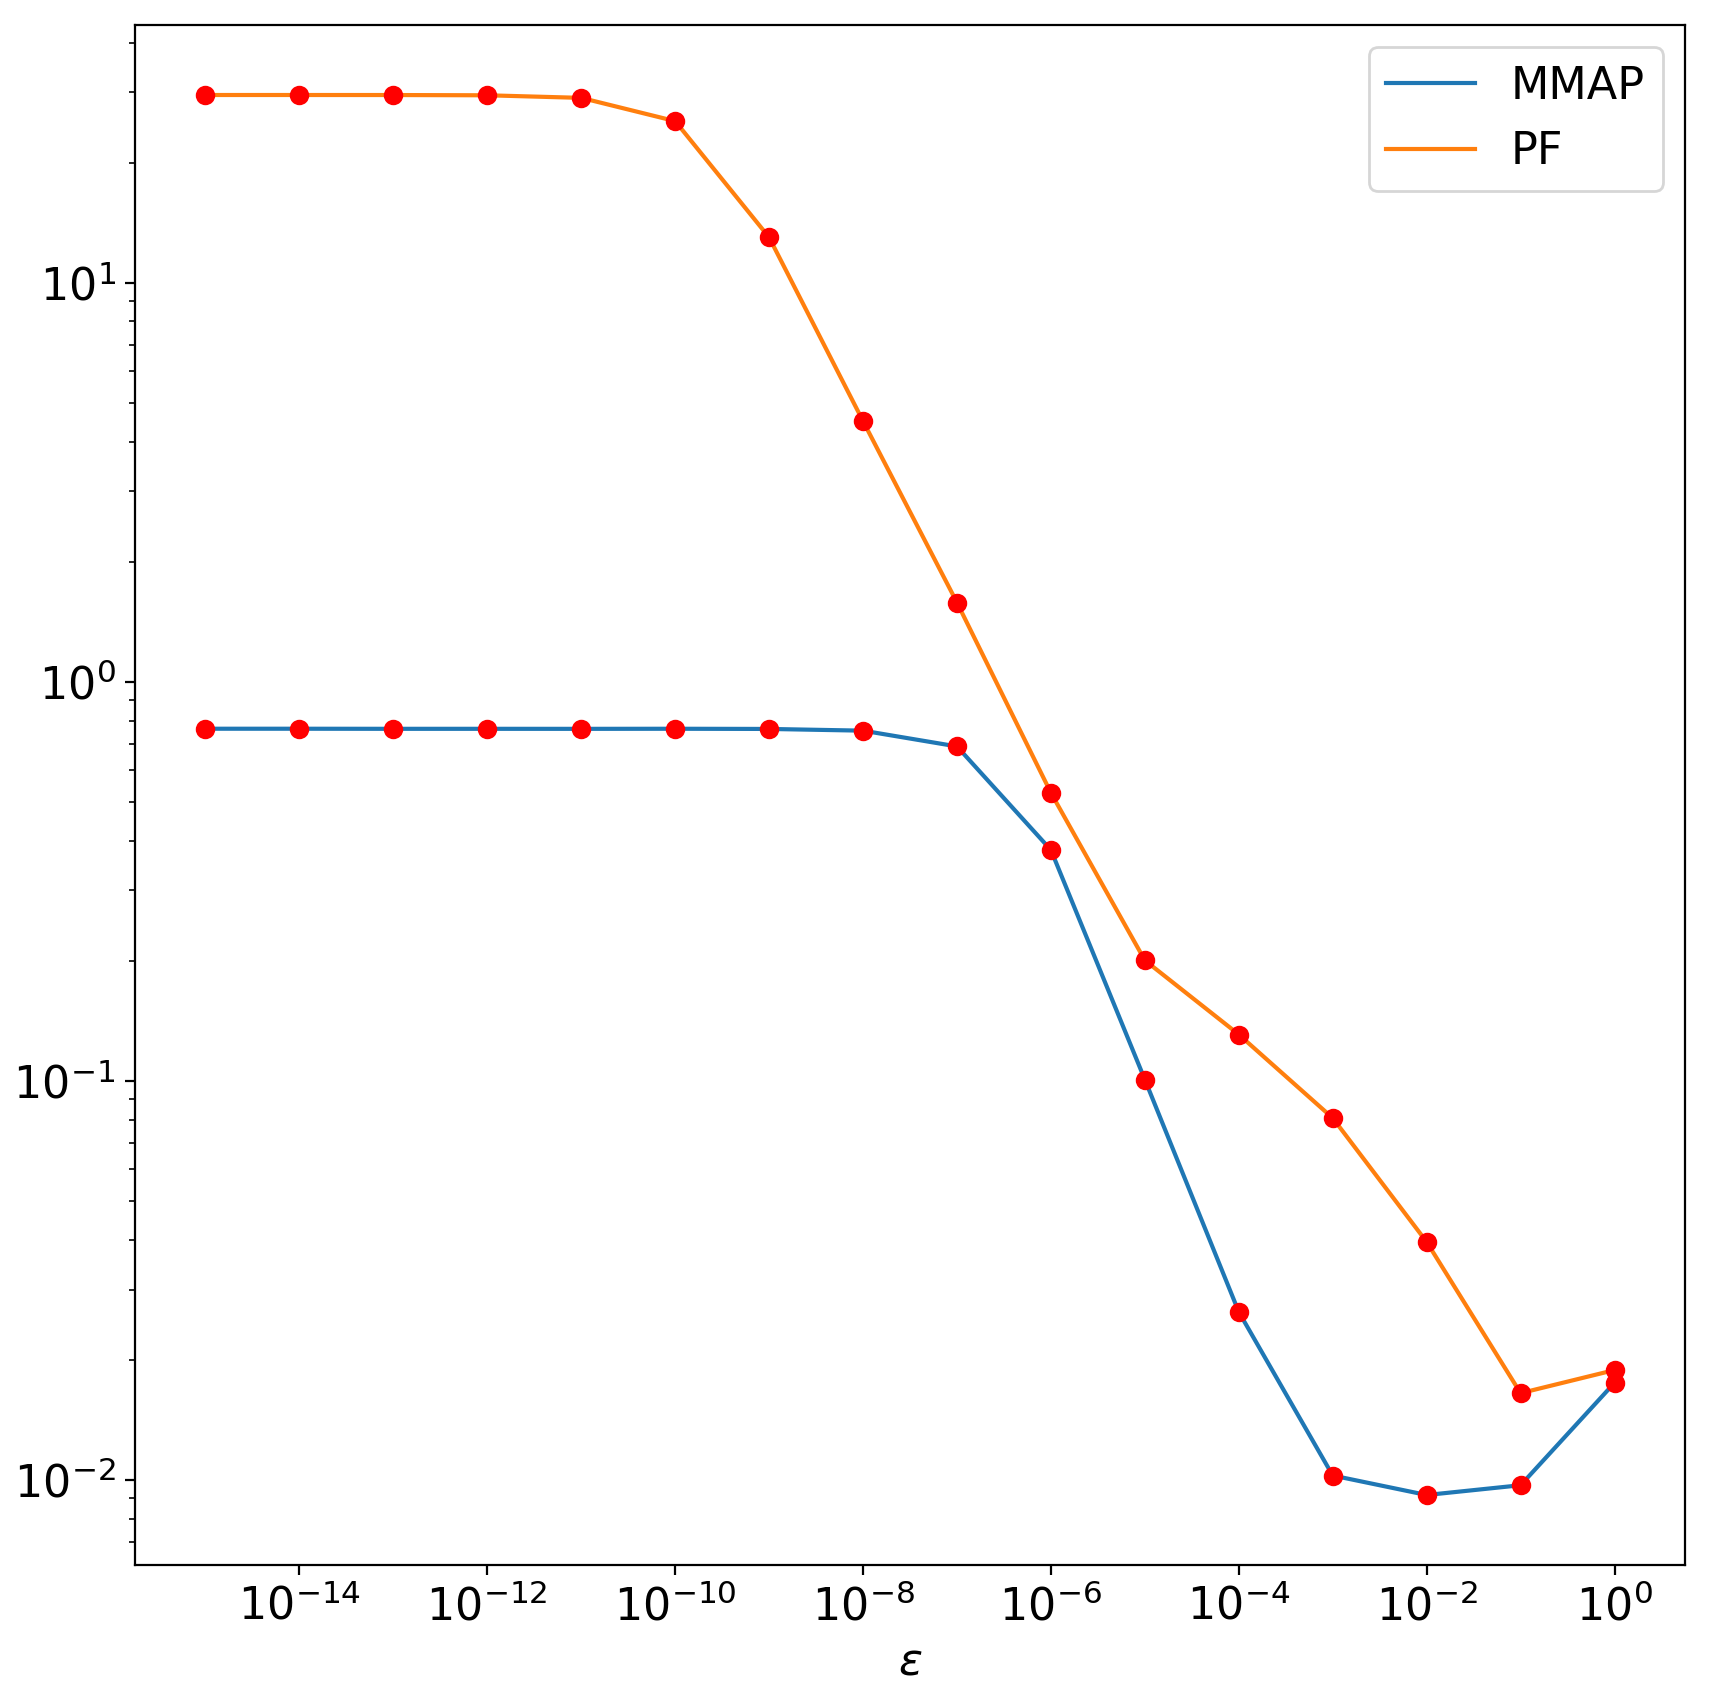
\includegraphics[width=\textwidth]{Pics/LHSims/E2/E2_NormalH1.png}
     \caption{H1 Error} \label{E2_LH_H1}
 \end{subfigure}
 \begin{subfigure}{0.42\textwidth}
     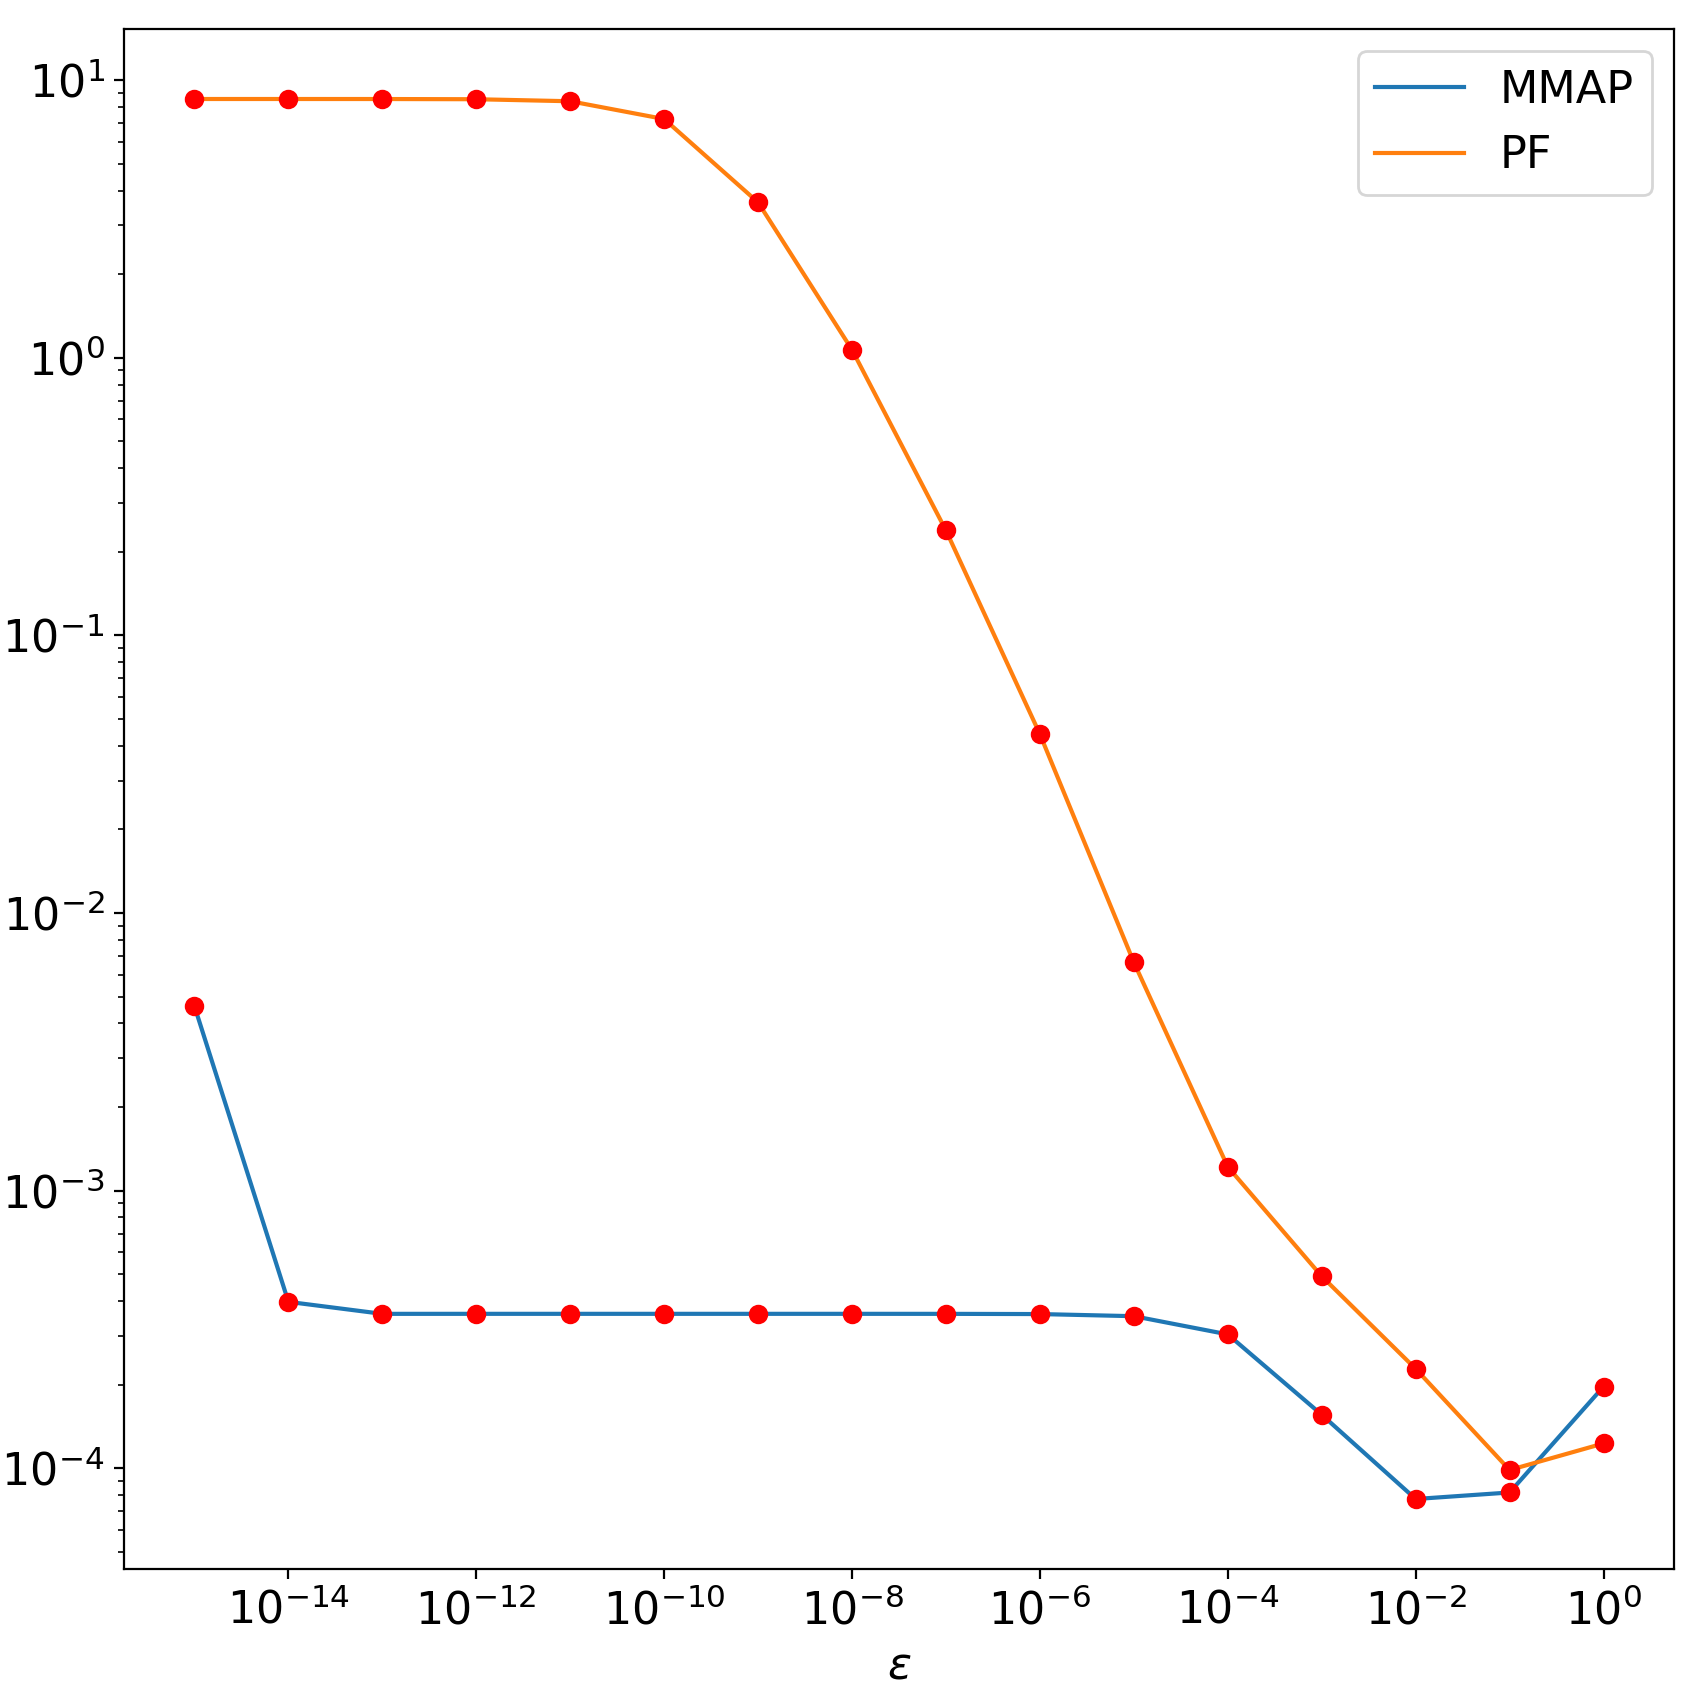
\includegraphics[width=\textwidth]{Pics/LHSims/E2/E2_INL2.png}
     \caption{L2 Error, with constraint} \label{E2_LH_L2_CON}
 \end{subfigure}
 \begin{subfigure}{0.42\textwidth}
     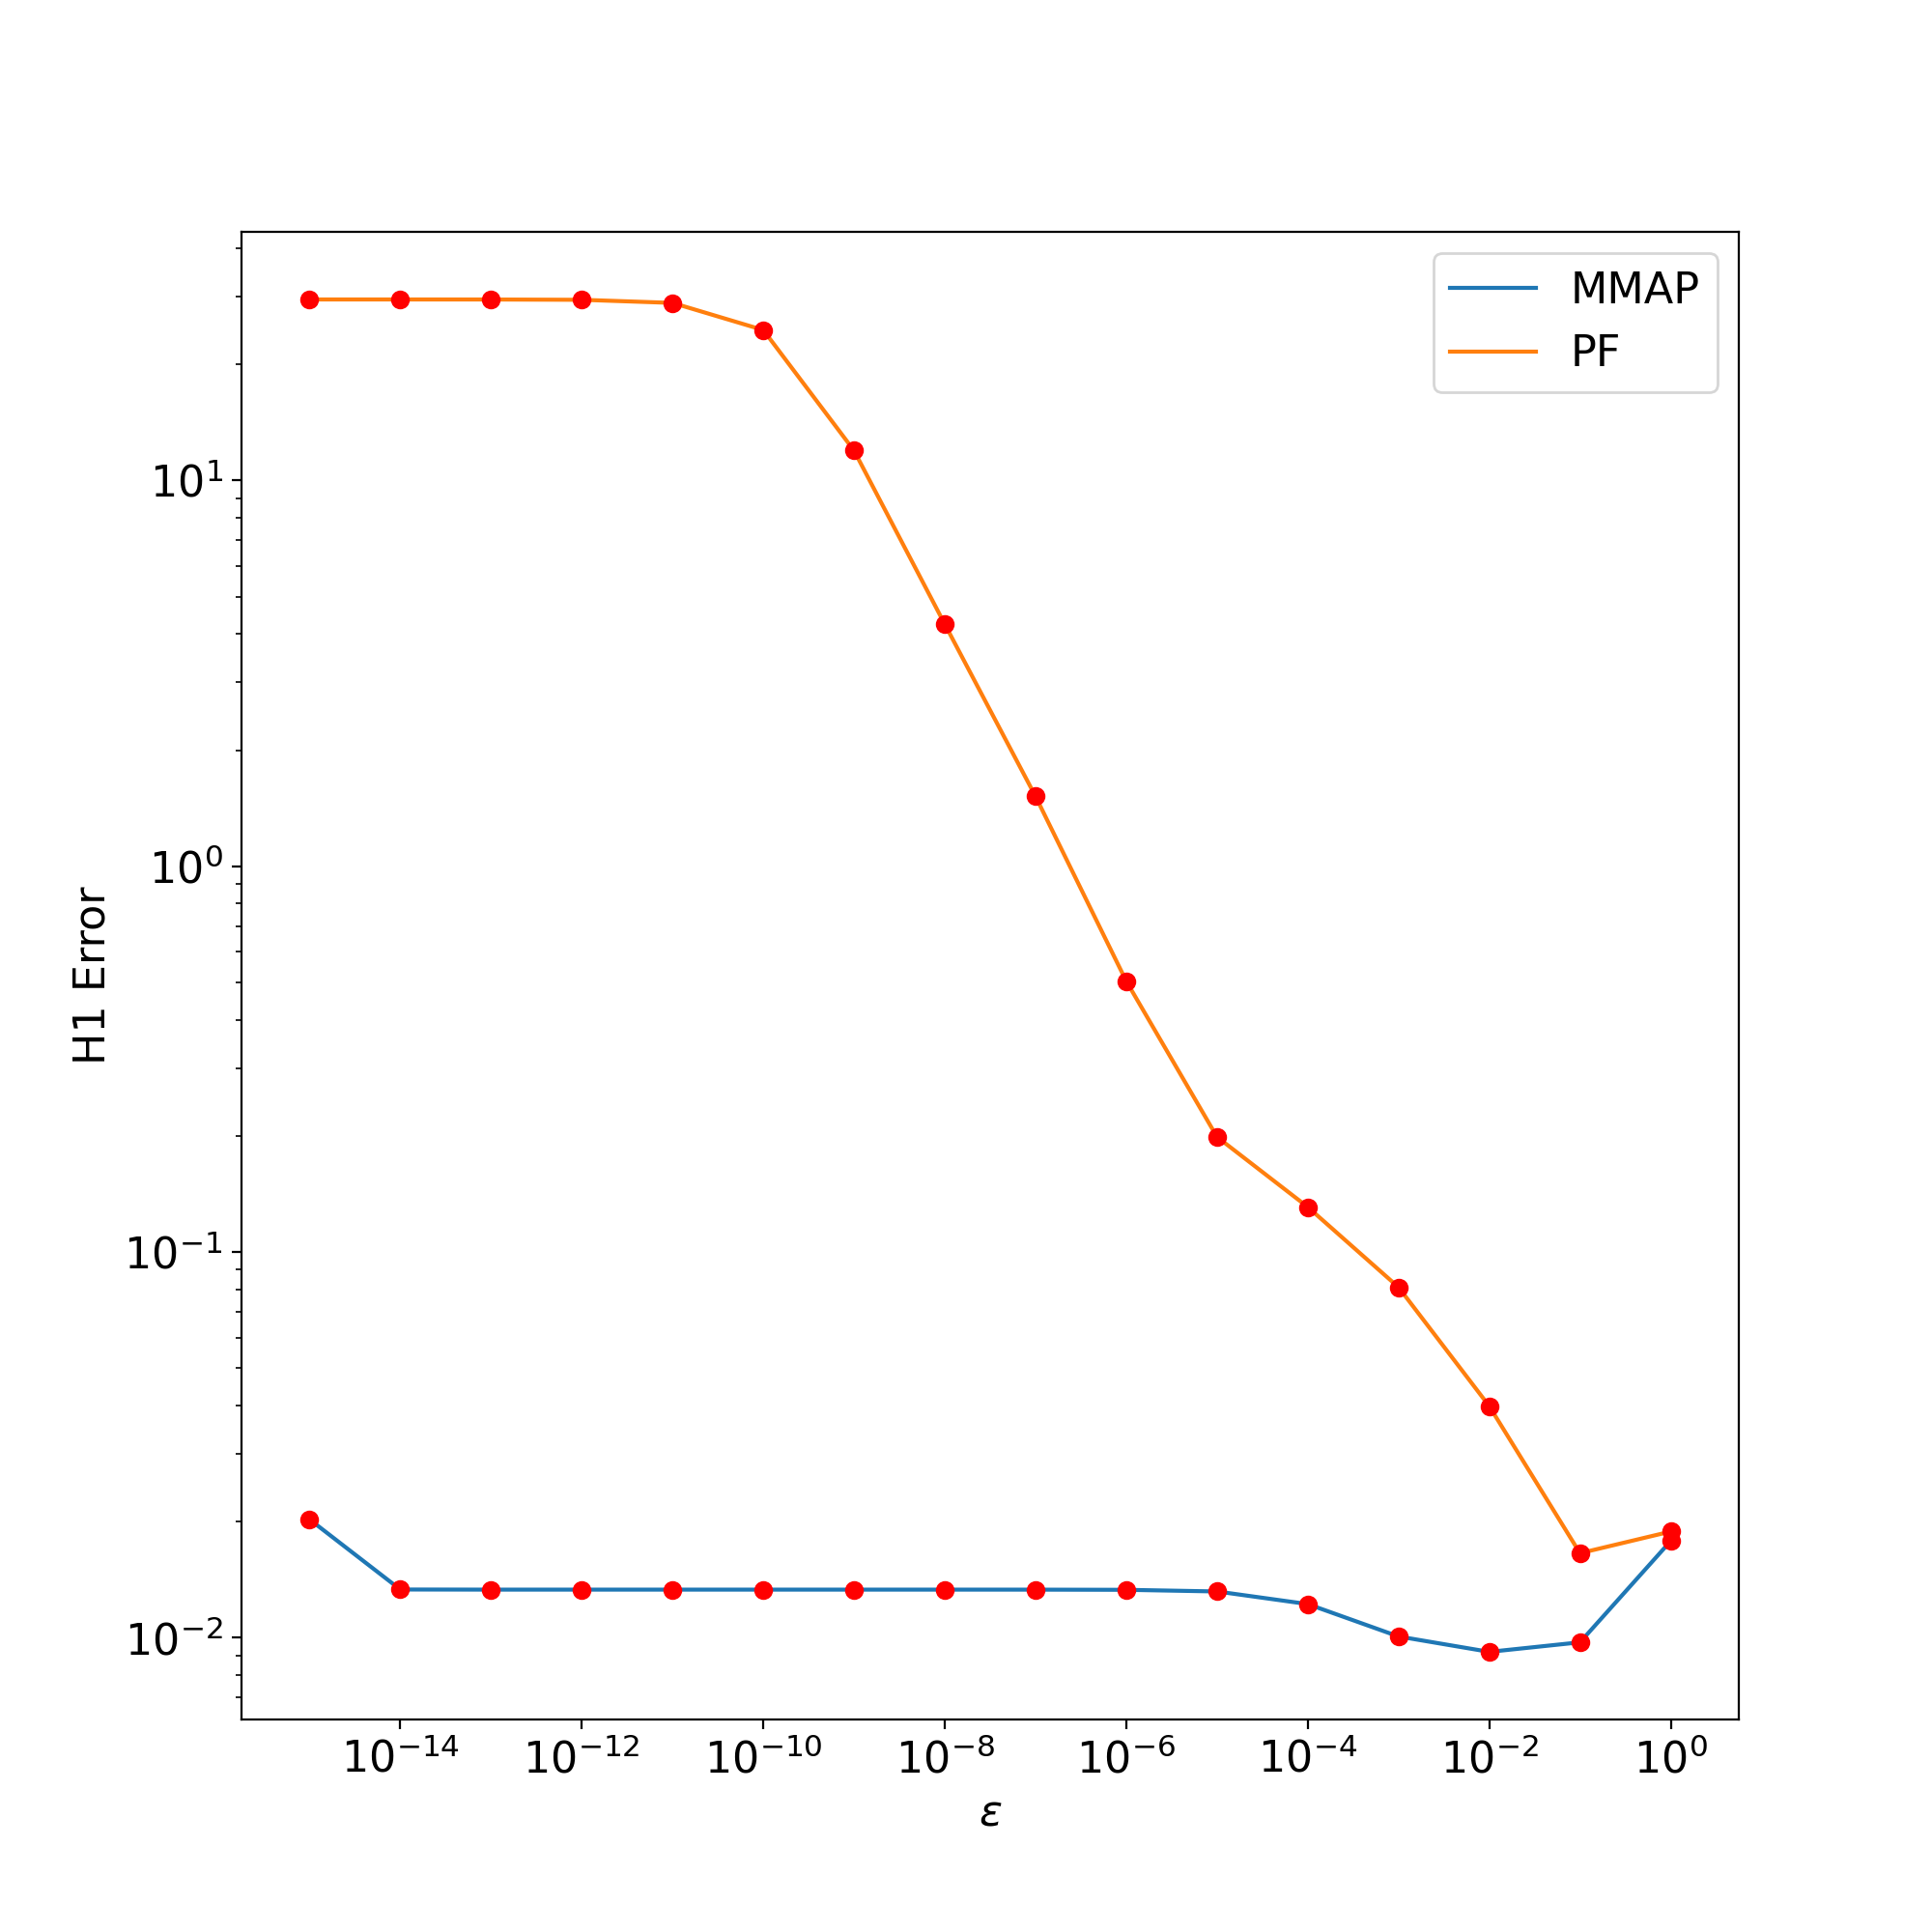
\includegraphics[width=\textwidth]{Pics/LHSims/E2/E2_INH1.png}
     \caption{H1 Error, with constraint} \label{E2_LH_H1_CON}
 \end{subfigure}
 \begin{subfigure}{0.42\textwidth}
     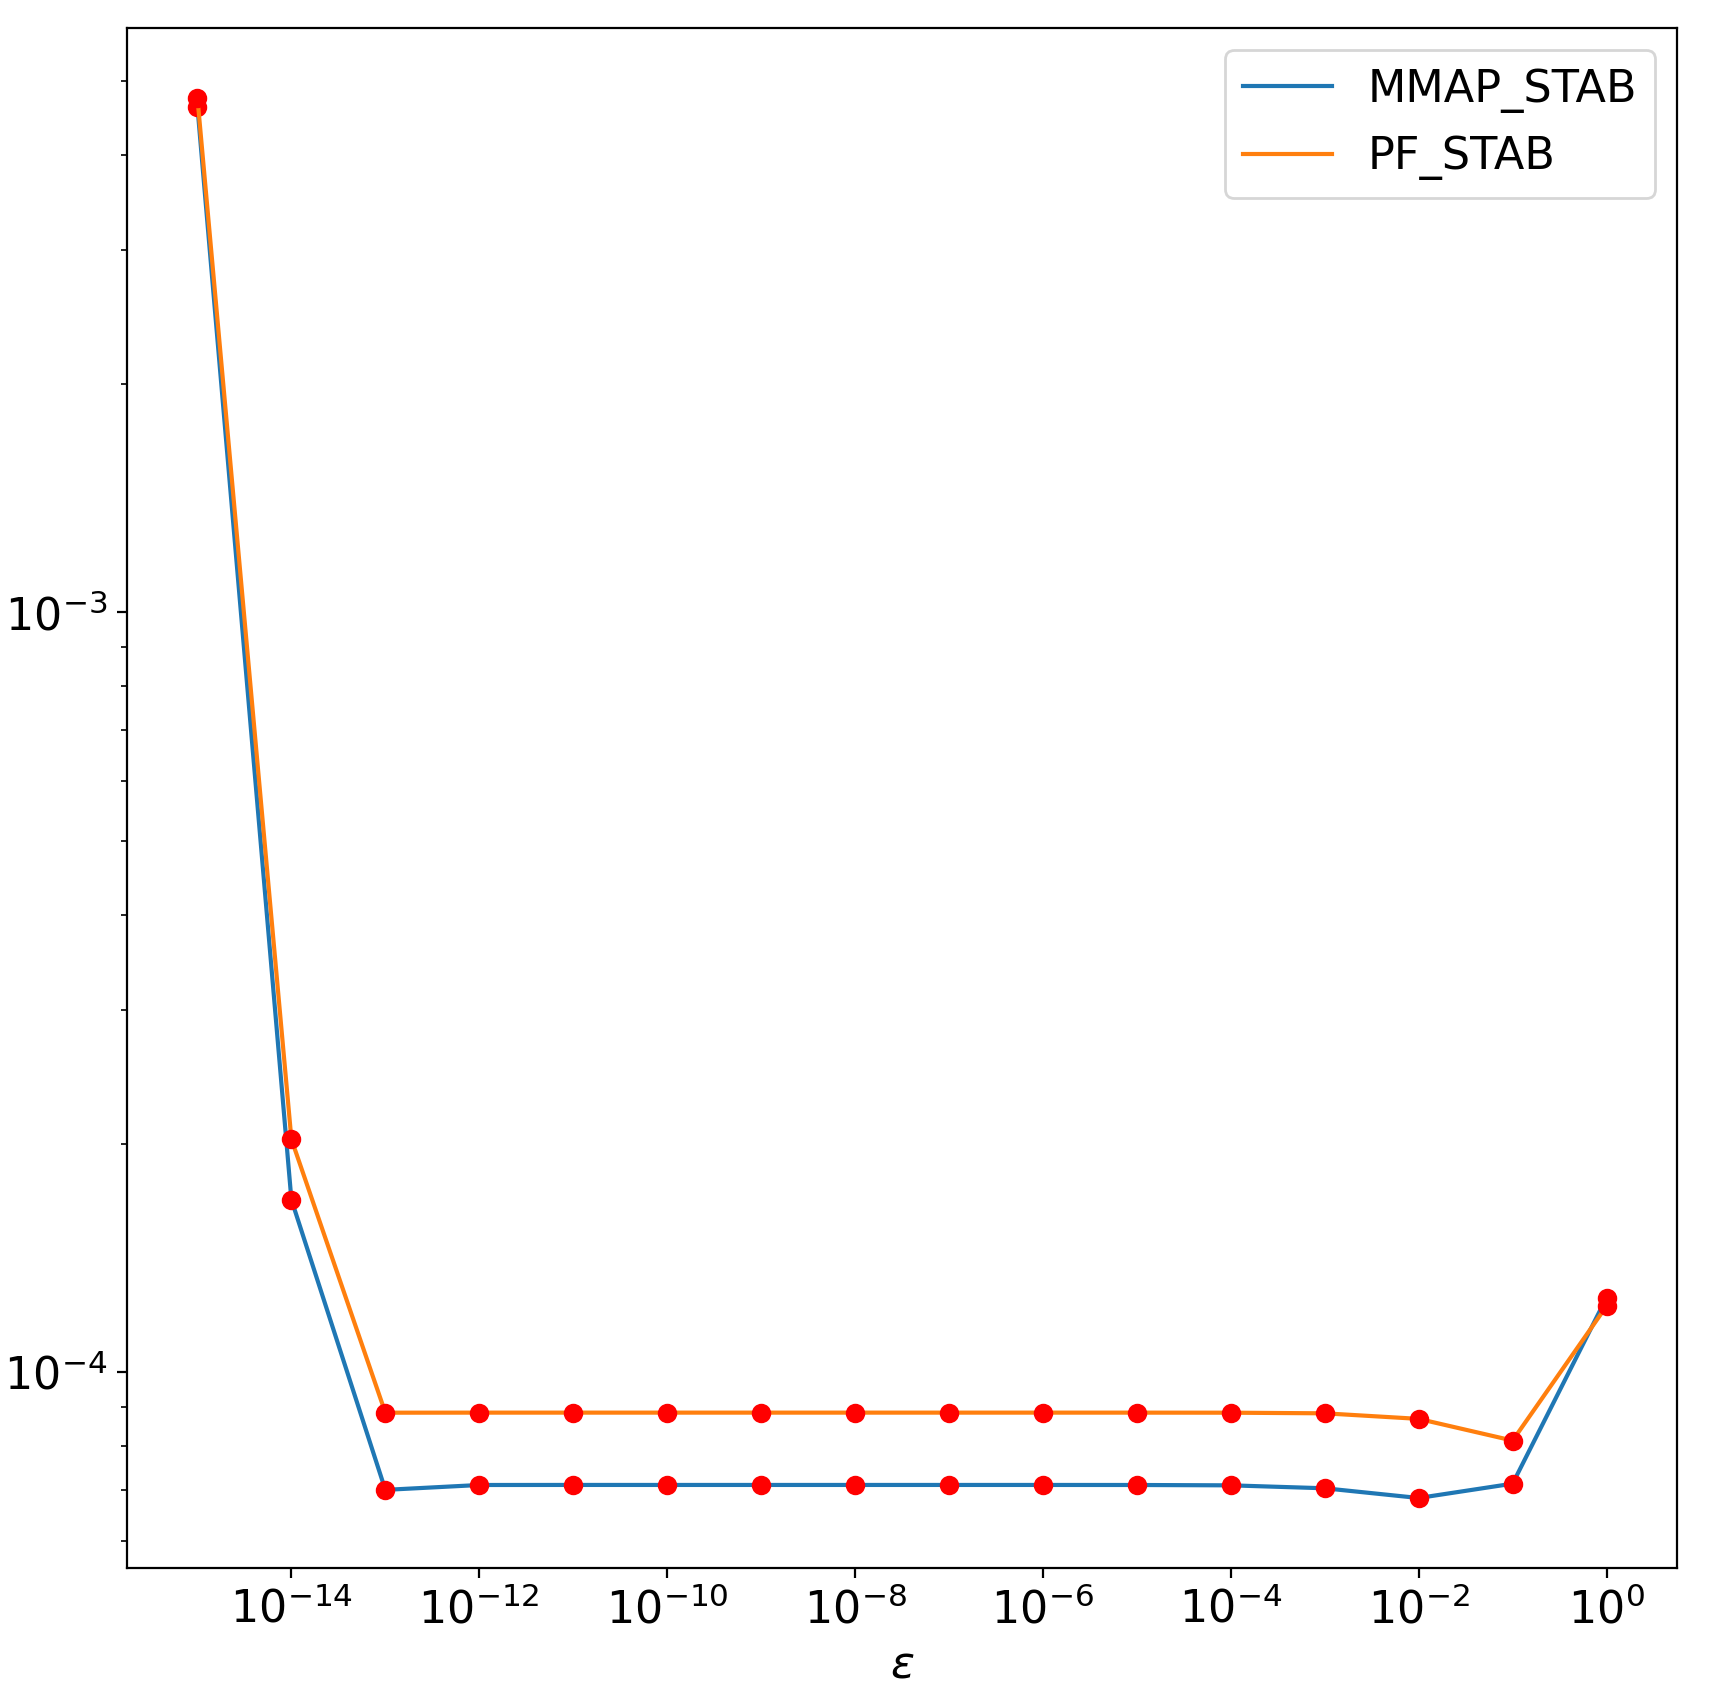
\includegraphics[width=\textwidth]{Pics/LHSims/E2/E2_STABL2.png}
     \caption{L2 Error, with stabilisation} \label{E2_LH_L2_STAB}
 \end{subfigure}
 \hfill
 \begin{subfigure}{0.42\textwidth}
     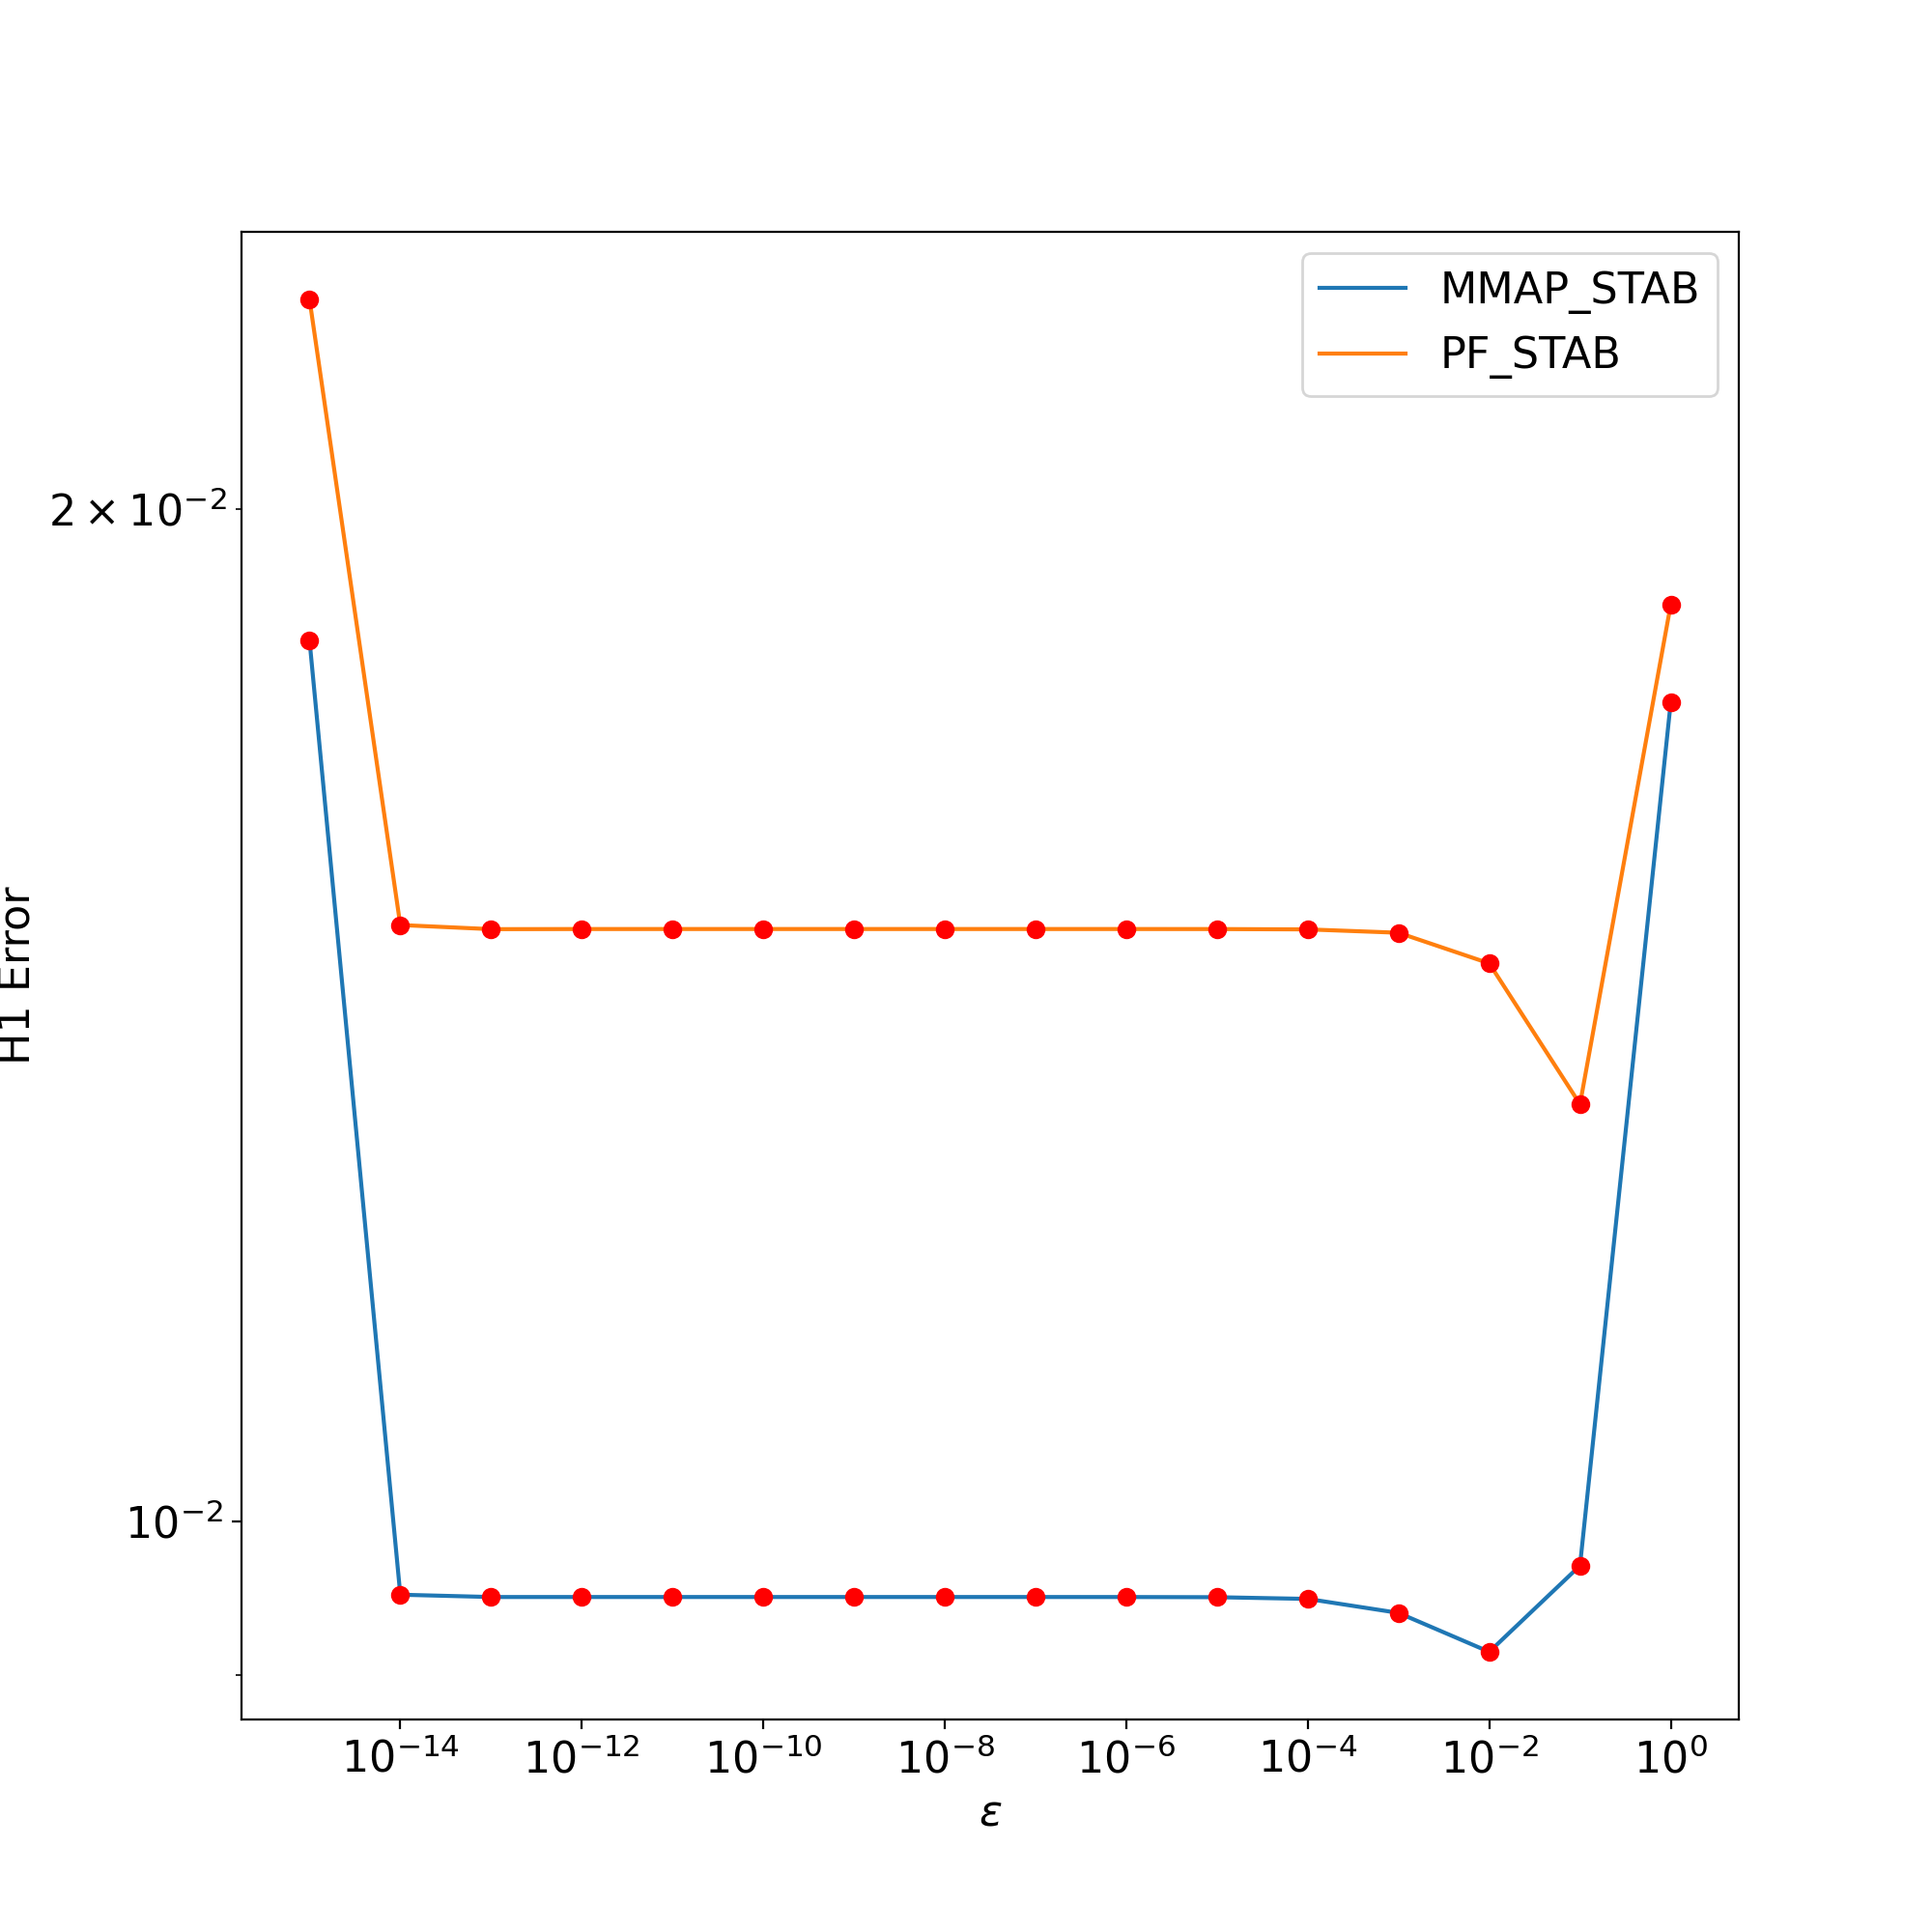
\includegraphics[width=\textwidth]{Pics/LHSims/E2/E2_STABH1.png}
     \caption{H1 Error, with stabilisation} \label{E2_LH_H1_STAB}
 \end{subfigure}
 \caption{Numerical demonstration for solver $(MMAP), (MMAP\_STAB), (PF)$ and $(PF\_STAB)$ on a $20\times 20$ quadrilateral grid using CG order $2$ for Example $2$. Also, $x=\varepsilon$ and $y=$ Error.} \label{E2_LH}
\end{figure}

\section{Example 3, Magnetic Islands}
We now solve an example on a square domain with non-zero boundary conditions on $\Gamma_D$ and with closed and open field lines. We will solve the PDE (\ref{PDE}) with $\Omega = [0,1]^2, \Gamma_D = \{y=0 \text{ or } y=1\}$ and $\Gamma_N = \{x=0 \text{ or } x=1\}$. We choose a magnetic field such 
\begin{equation}
\mathbf{b} = \frac{\mathbf{B}}{|\mathbf{B}|}, 
\mathbf{B} = \left[ \begin{matrix}
-\cos(\pi y)\\
4a \sin(4 \pi x)
\end{matrix} \right]
\end{equation}
which is visualised in Figure \ref{E3_VF}. Additionally, after some ODE analysis, we get the streamlines for this vector field are
\begin{equation}
\sin(\pi y)-a\cos(4\pi x) = C,
\end{equation}
with $-a\leq C \leq 1+a$.
\begin{figure}[H]
\begin{center}
 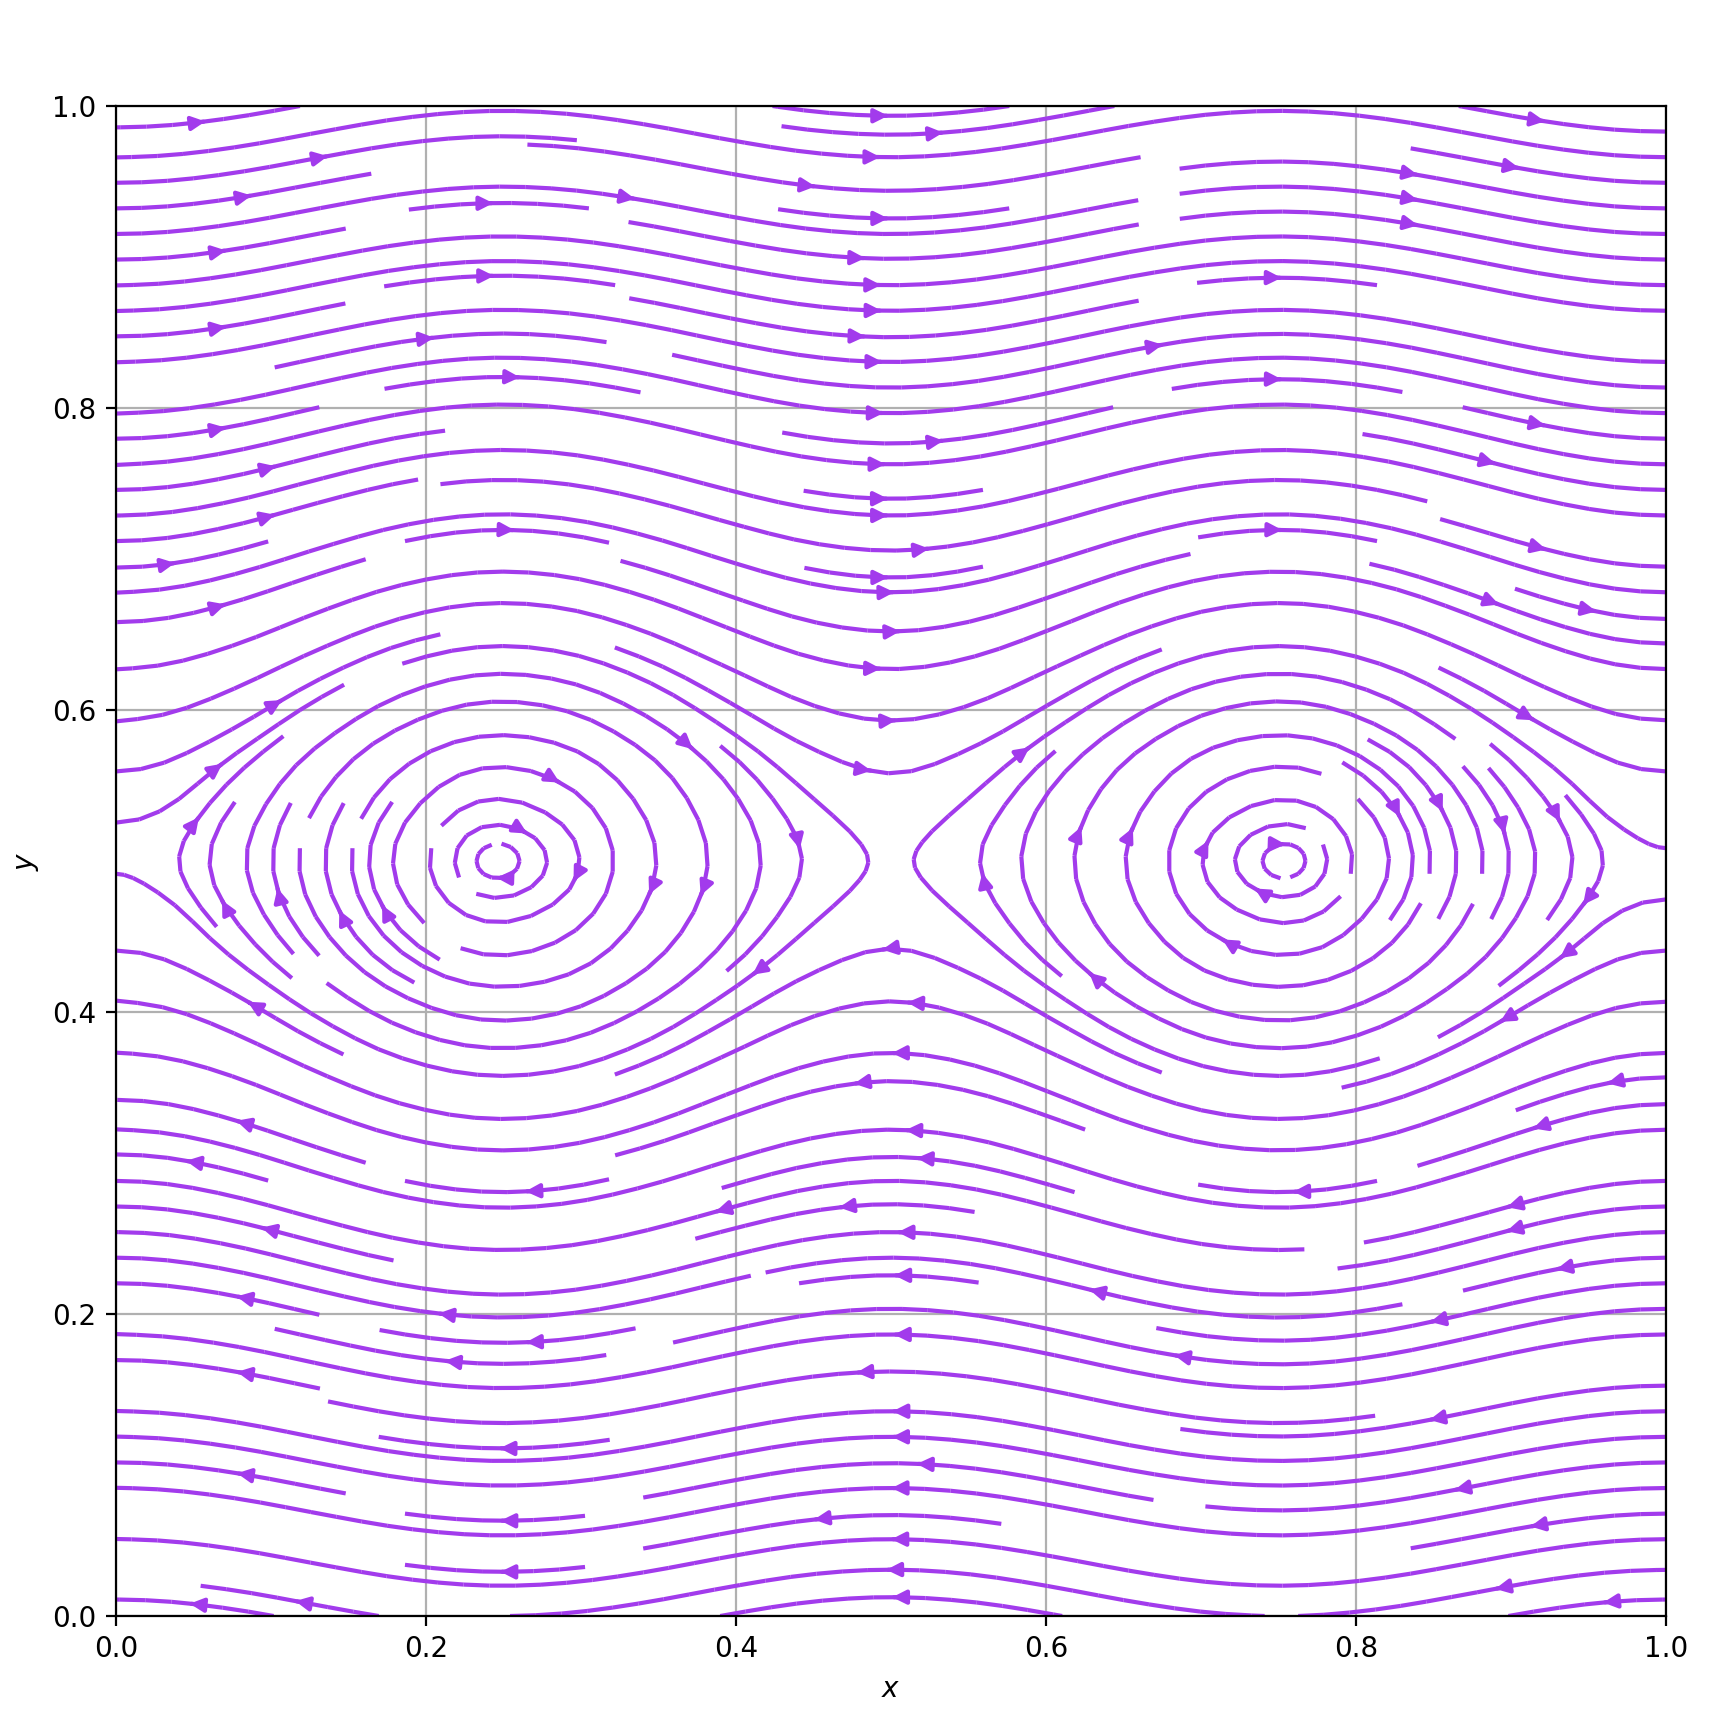
\includegraphics[width=0.85\textwidth]{Pics/VectorField/E3b.png}
  \caption{Electromagnetic field $\mathbf{b}$ for Example $3$.}
 \label{E3_VF}
\end{center}
\end{figure}

 This example was proposed by \cite{DN} but it does not satisfy the restrictions we impose. The restrictions are $\mathbf{b} \cdot \mathbf{n} = 0$ on $\Gamma_D$ this failed restriction can be seen in Figure \ref{E3_VF} and $u = 0$ on $\Gamma_D$ this failed restriction can be seen in Figure \ref{E3_u}. Thus, our numerical solvers will struggle to solve this example, this problem is rectified by in Example $4$. Additionally, \cite{DN} rectified this problem by defining $\Gamma_D := \{\mathbf{x} \in \partial \Omega :  \mathbf{b} \cdot \mathbf{n} = 0\}$.

We will use the exact solution
\begin{equation}
u = \sin(10\sin(\pi y)-10a\cos(4 \pi x)) + \varepsilon \cos(2 \pi x)\sin(10 \pi y)
\end{equation}
which is visualised with its source term $f$ in Figure \ref{E3_uf} at $\varepsilon = 10^{-10}$. Additionally, we visualise this for $\varepsilon = 0.1$.
\begin{figure}[H]
 \begin{subfigure}{0.5\textwidth}
     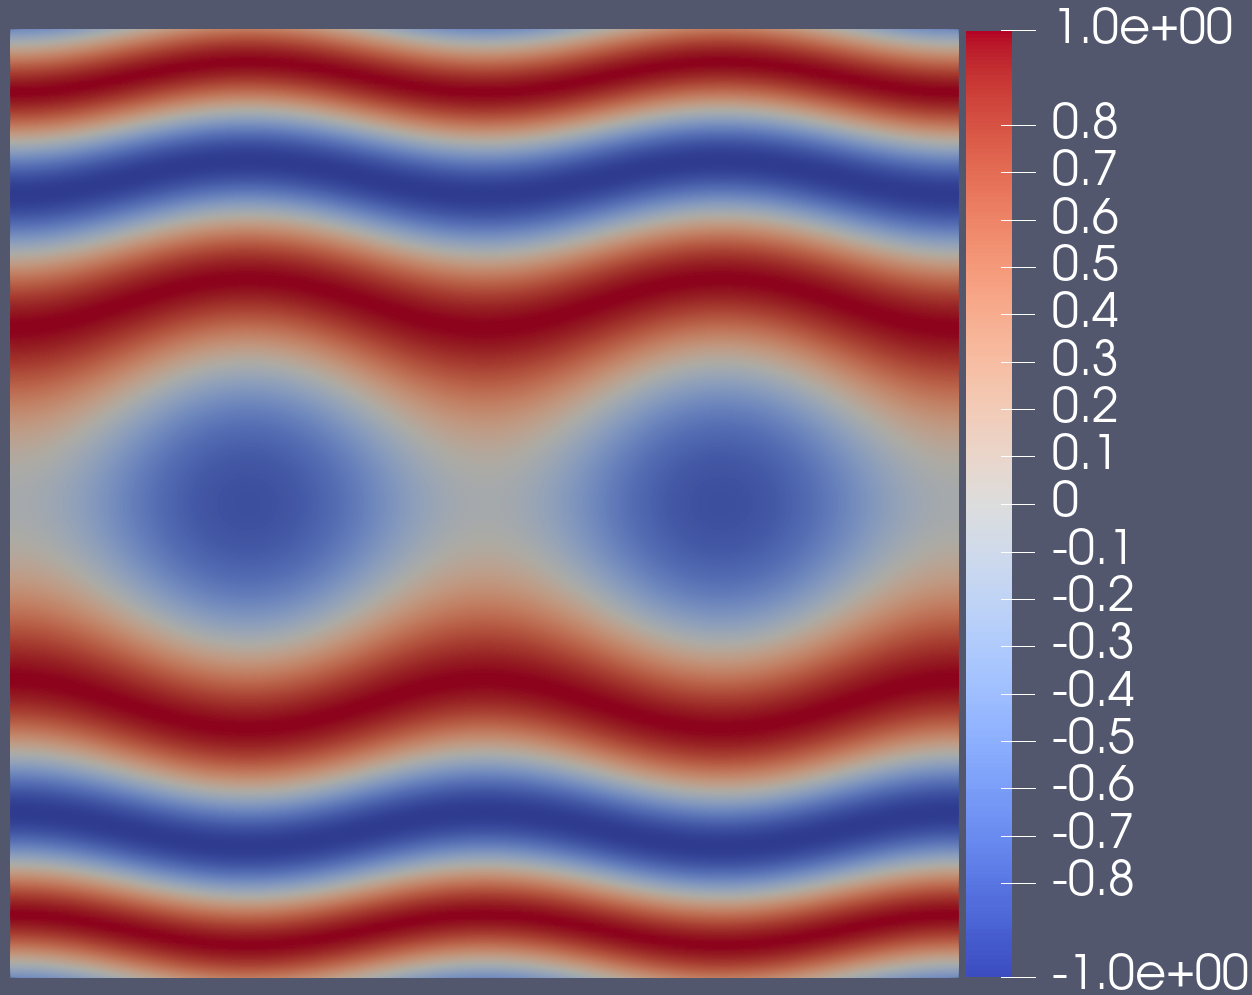
\includegraphics[width=\textwidth]{Pics/uf/U_E3_eps_10.png}
     \caption{Exact solution $u$.} \label{E3_u}
 \end{subfigure}
   \begin{subfigure}{0.5\textwidth}
     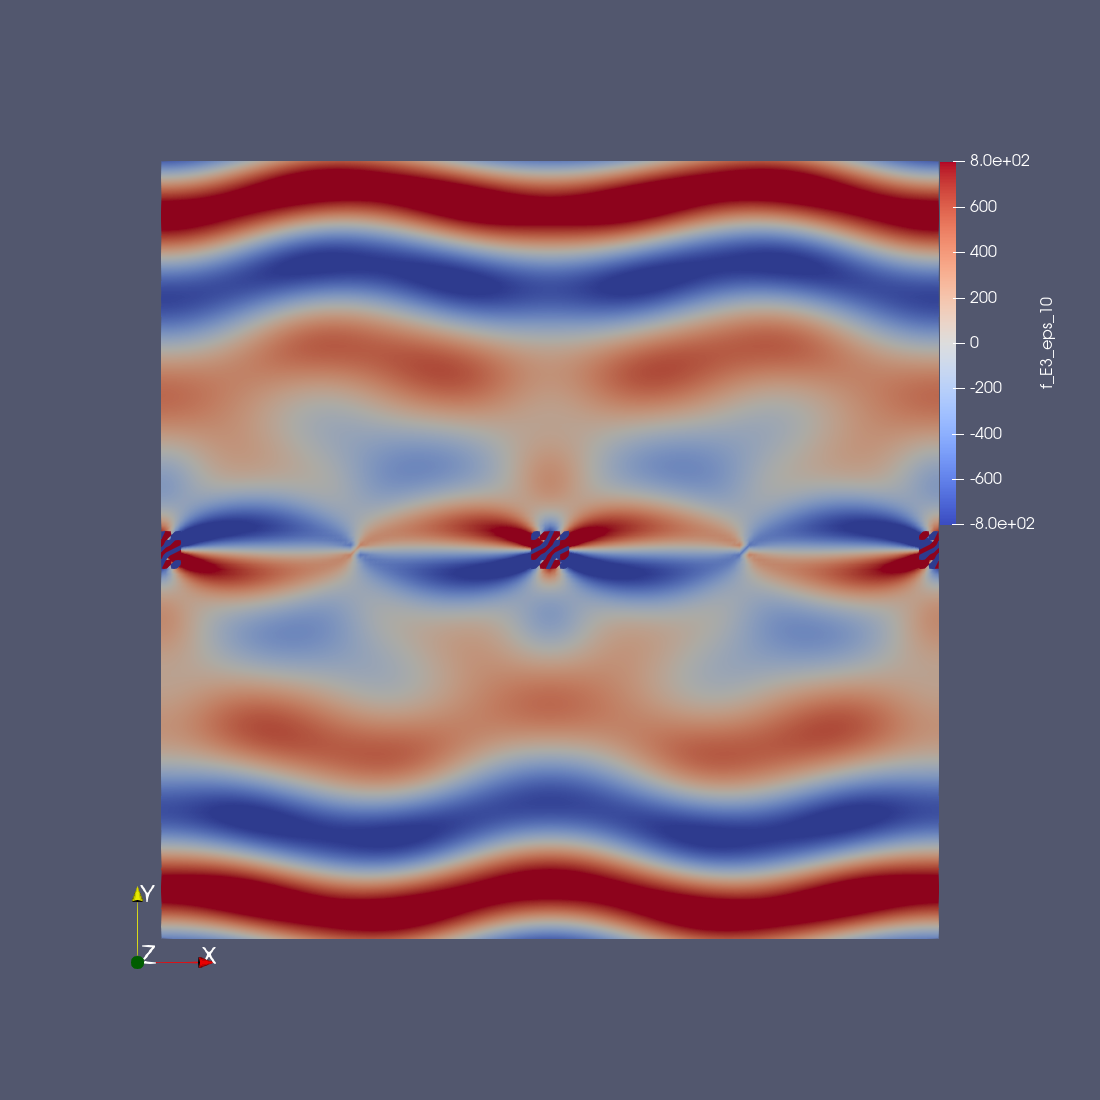
\includegraphics[width=\textwidth]{Pics/uf/F_E3_eps_10.png}
     \caption{Source term $f$.}
 \end{subfigure}
 \caption{Example $3$ with $\varepsilon = 10^{-10}$.} \label{E3_uf}
\end{figure}
\begin{figure}[H]
 \begin{subfigure}{0.5\textwidth}
     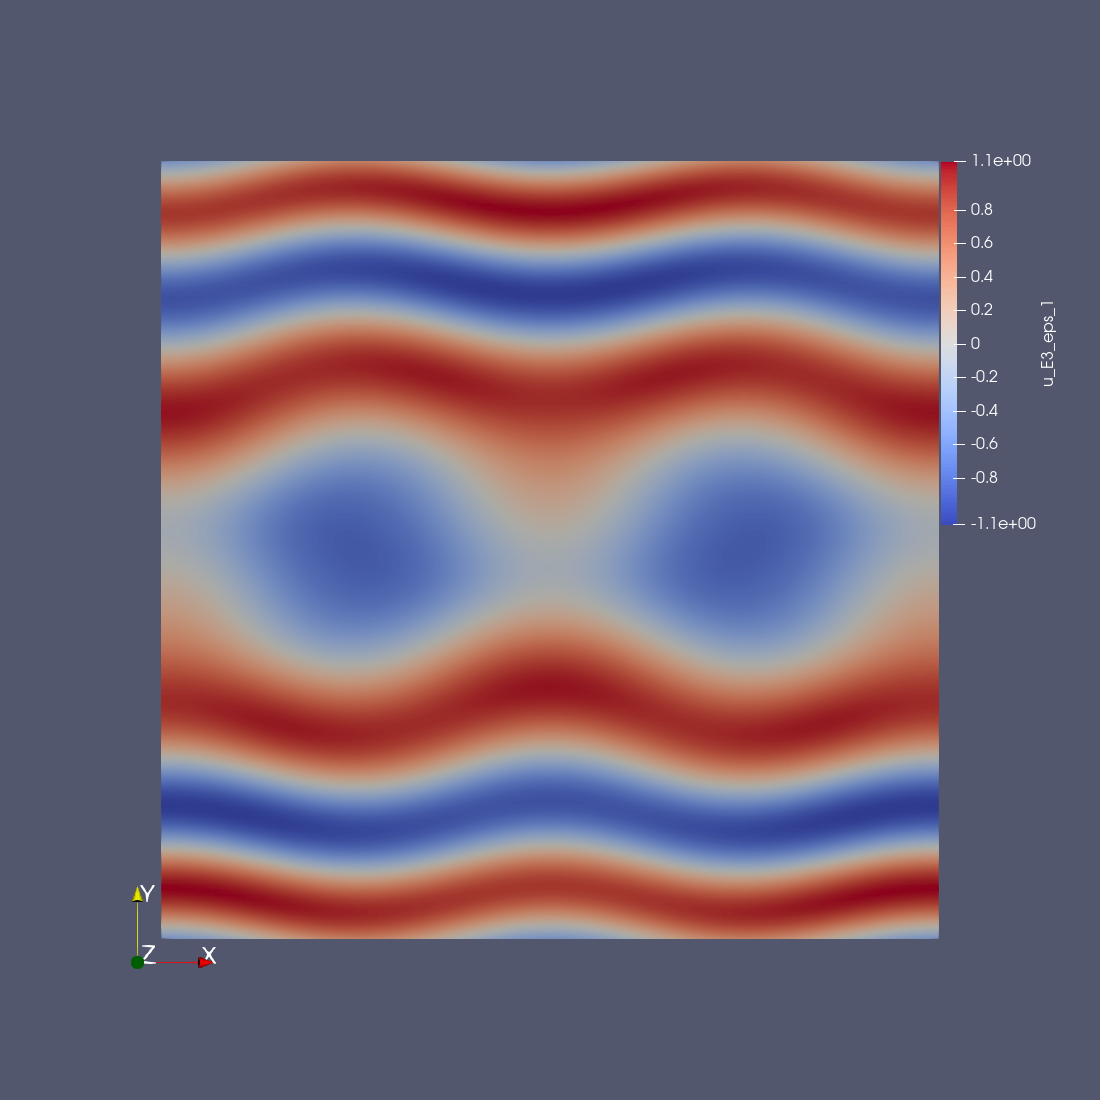
\includegraphics[width=\textwidth]{Pics/uf/U_E3_ep1.png}
     \caption{Exact solution $u$.}
 \end{subfigure}
   \begin{subfigure}{0.5\textwidth}
     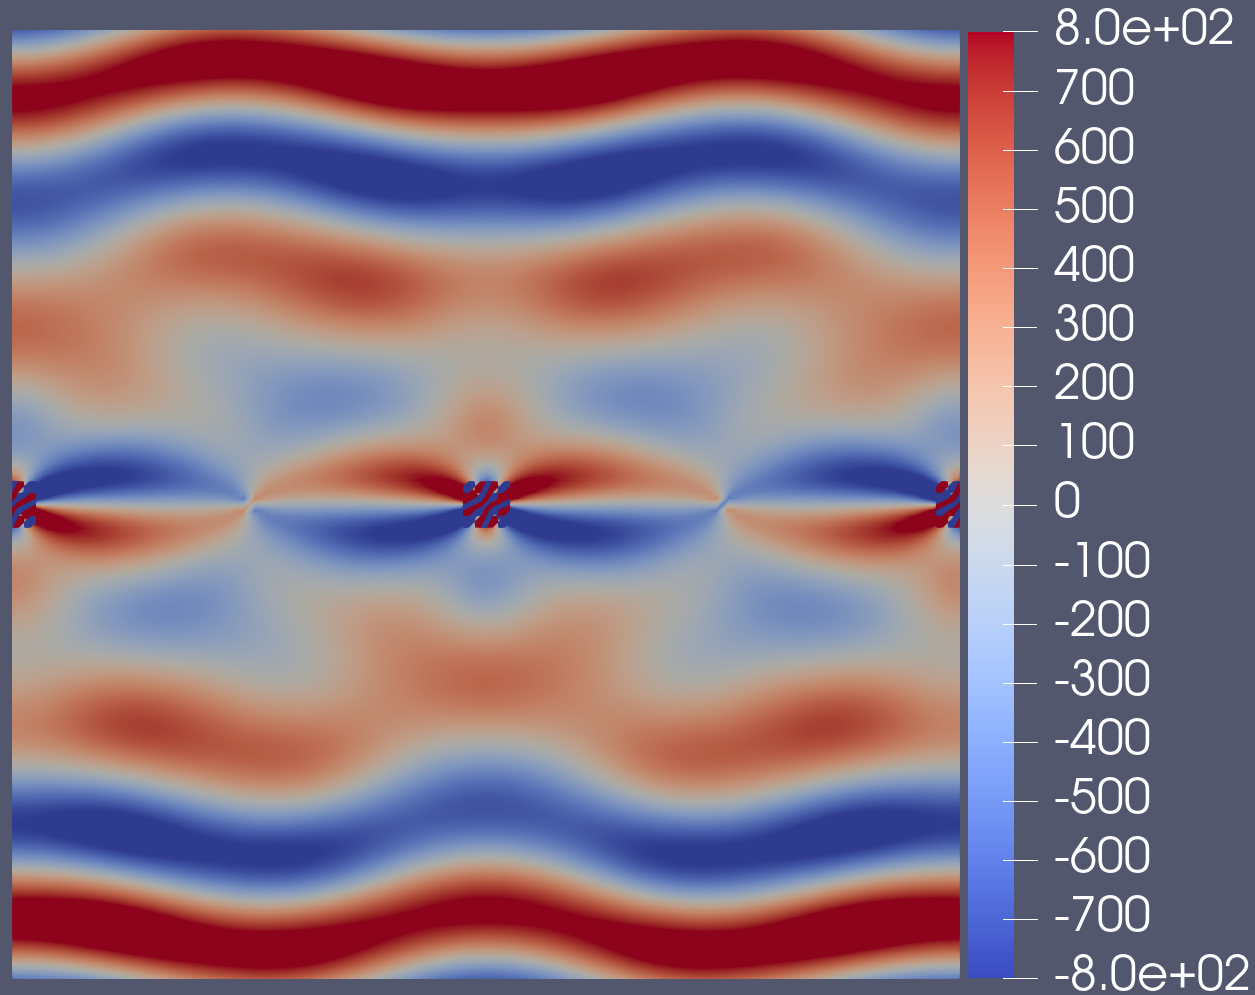
\includegraphics[width=\textwidth]{Pics/uf/F_E3_eps_1.png}
     \caption{Source term $f$.}
 \end{subfigure}
 \caption{Example $3$ with $\varepsilon = 0.1$.} \label{E3_uf_01}
\end{figure}


\begin{figure}[H]
 \begin{subfigure}{0.5\textwidth}
     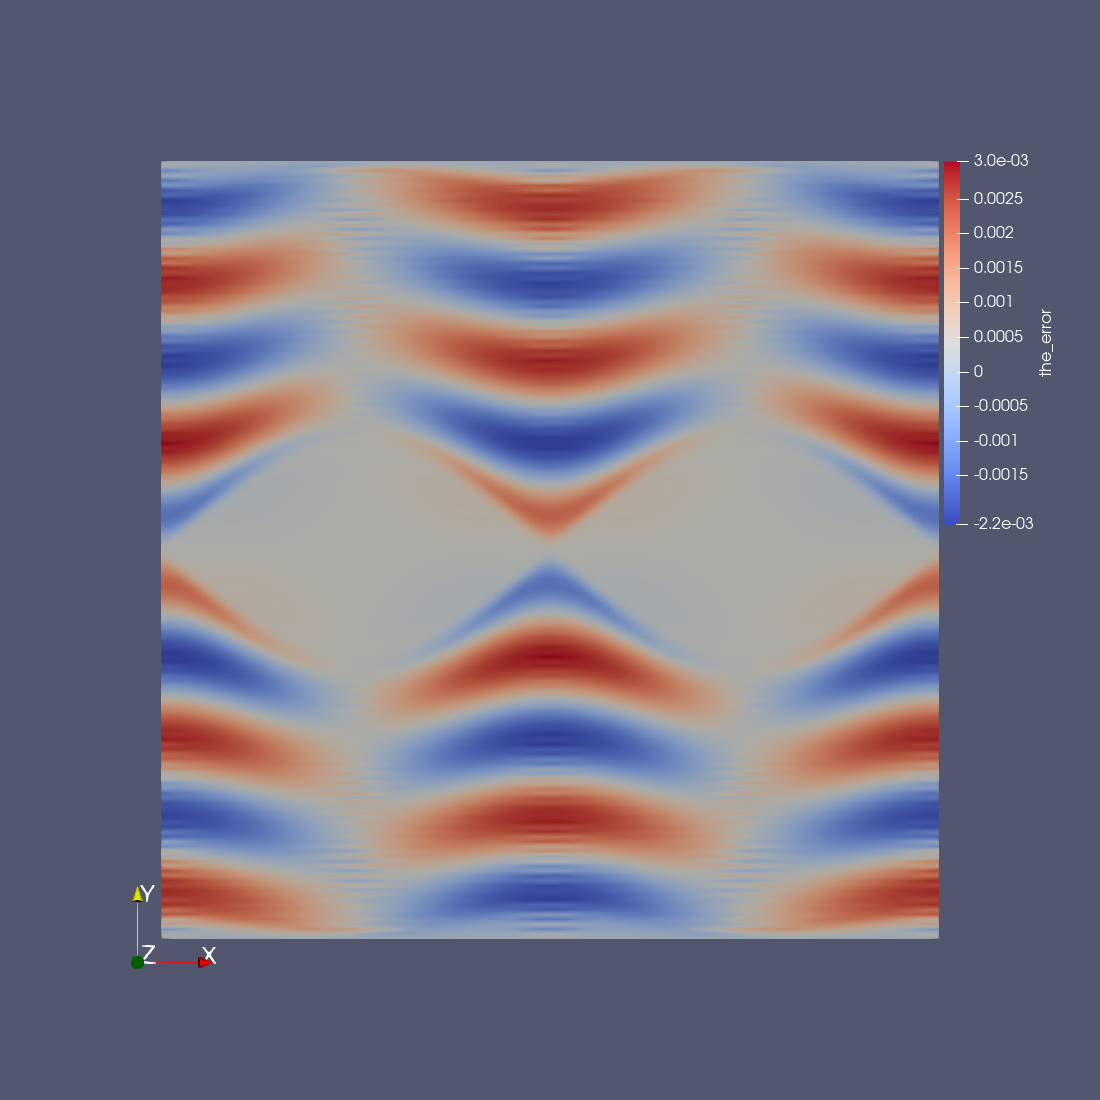
\includegraphics[width=\textwidth]{Pics/ErrorPlots/E3_MMAP_STAB.png}
     \caption{L2 $=2.6\times10^{-2}$ for $(MMAP\_STAB)$}
 \end{subfigure}
   \begin{subfigure}{0.5\textwidth}
     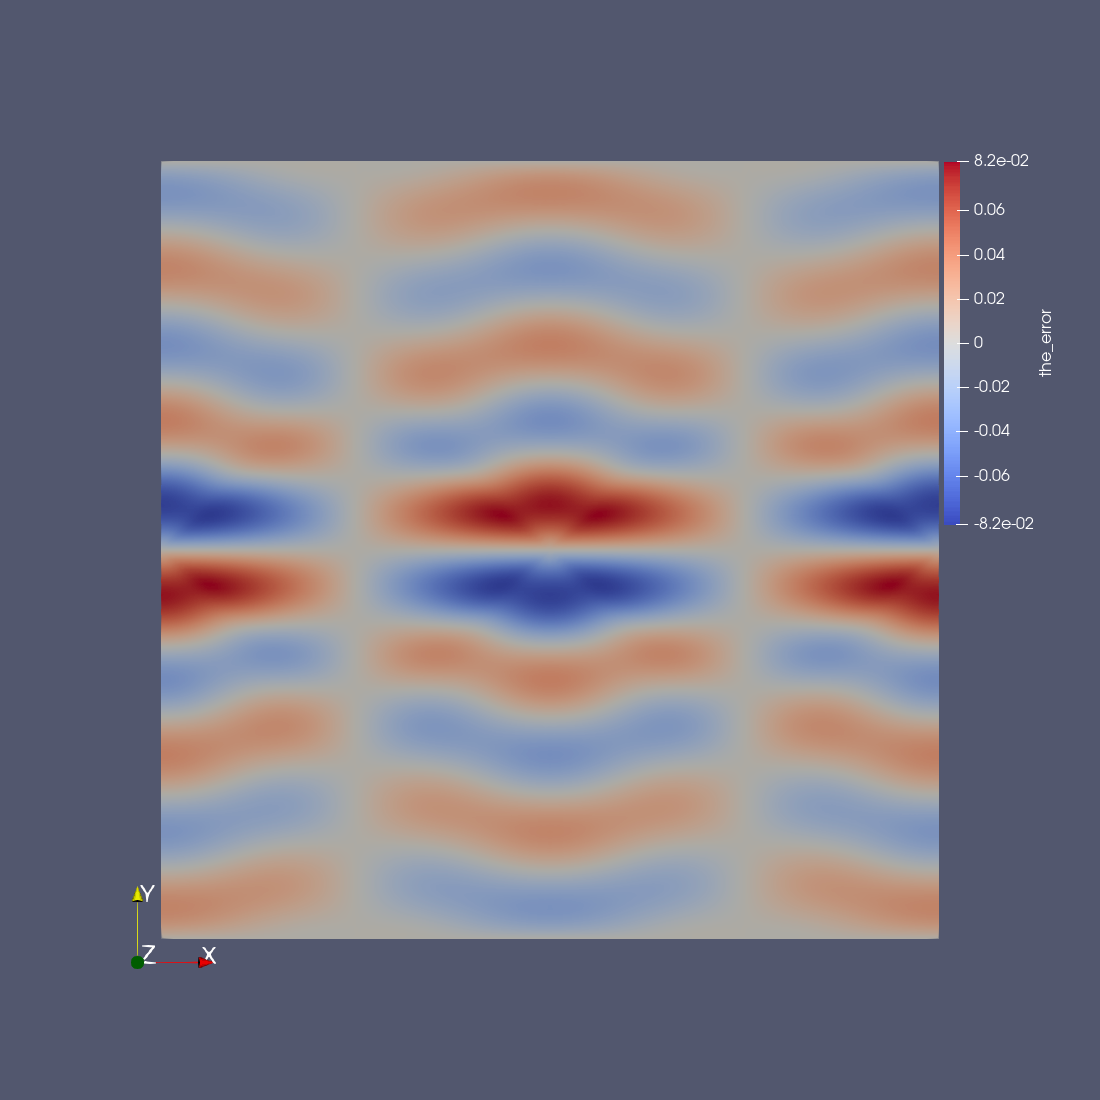
\includegraphics[width=\textwidth]{Pics/ErrorPlots/E3_PF_STAB.png}
     \caption{L2 $=2.6\times10^{-2}$ for $(PF\_STAB)$}
 \end{subfigure}
 \caption{Visualisation of Error $u_e-u_h$ for Example $3$ with $\varepsilon = 10^{-10}$, CG order $2$ on a $80 \times 80$ quadrilateral grid with dof$=51842$} \label{E3_Error}
\end{figure}


\begin{figure}[H]
 \begin{subfigure}{0.5\textwidth}
     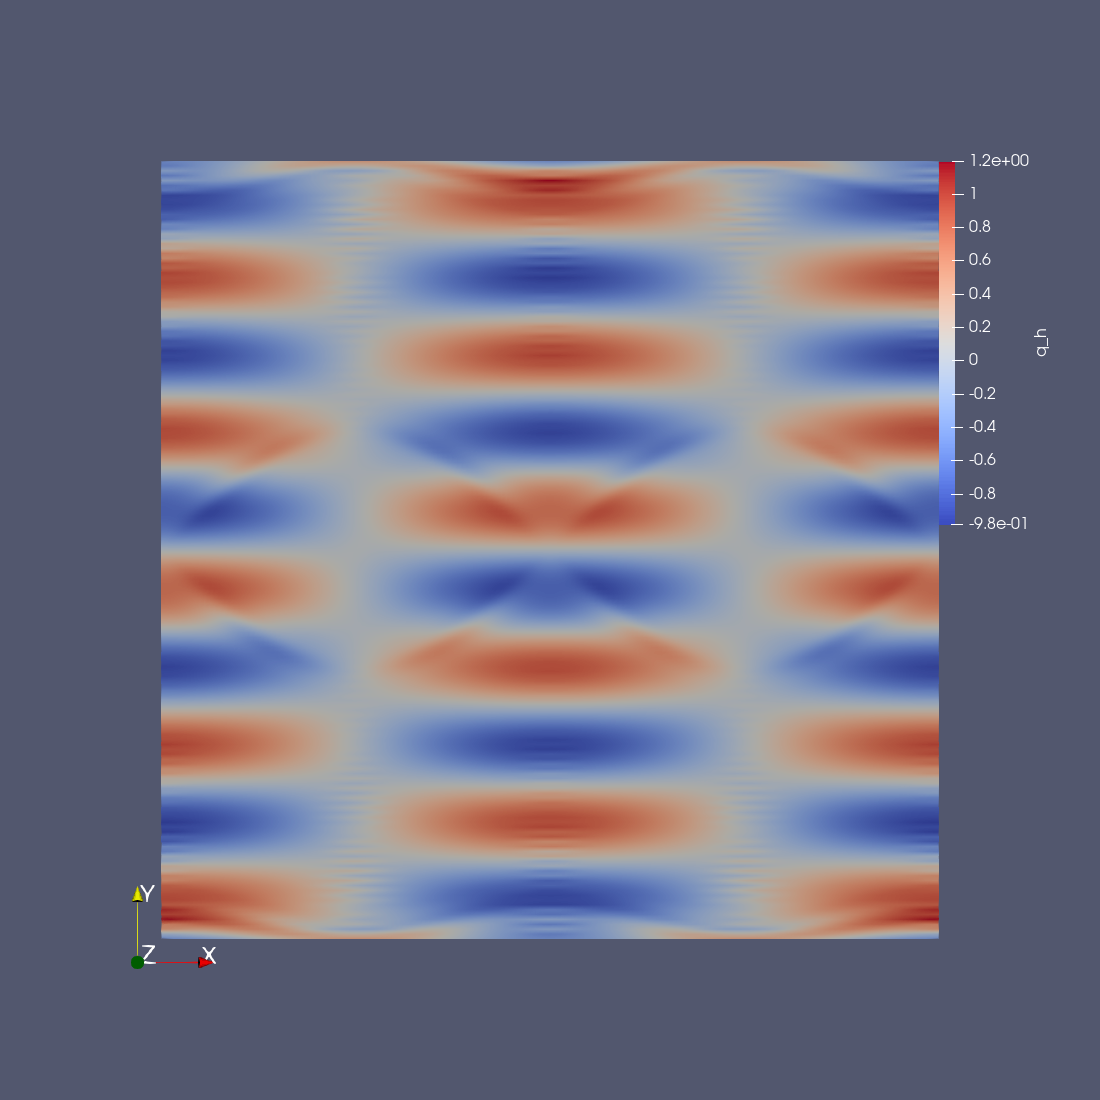
\includegraphics[width=\textwidth]{Pics/ErrorPlots/E3_MMAP_STAB_Q.png}
     \caption{Solves $q$ defined in equation (\ref{MMAP_STAB_w}) for $(MMAP\_STAB)$}
 \end{subfigure}
   \begin{subfigure}{0.5\textwidth}
     \includegraphics[width=\textwidth]{Pics/ErrorPlots/E3_PF_STAB_Q.png}
     \caption{Solves $q$ defined in equation (\ref{PF_STAB_w}) for $(PF\_STAB)$}
 \end{subfigure}
 \caption{Visualisation of $q$ defined in sections \ref{MMAP_STAB} and \ref{PF_STAB} for Example $3$ with $\varepsilon = 10^{-10}$, CG order $2$ on a $80 \times 80$ quadrilateral grid with dof$=51842$.} \label{E3_Q}
\end{figure}

\newpage
\section{Example 4, Magnetic Islands}

We now introduce an example on a unit square where $\Gamma_D$ has zero boundary conditions. This is similar to Example $3$ but Example $4$ satisfies $\mathbf{b}\cdot\mathbf{n} = 0$ on $\Gamma_D$ this can be seen in Figure \ref{E4_VF}. This shows its vector field $\mathbf{b}$ on $y=0$ and $y=1$ is parallel to the boundary. Additionally, this has open and closed field lines.
Thus on $\Omega = [0,1]^2, \Gamma_D = \{y=0 \text{ or } y=1\}$ and $\Gamma_N = \{x=0 \text{ or } x=1\}$ we solve the PDE (\ref{PDE}) with the same magnetic
\begin{equation}
\mathbf{b} = \frac{\mathbf{B}}{|\mathbf{B}|}, 
\mathbf{B} = \left[ \begin{matrix}
-\cos(\pi y)\\
4a \sin(4 \pi x) \sin(\pi y)
\end{matrix} \right]
\end{equation}
where the electromagnetic field $\mathbf{b}$ is shown in Figure \ref{E4_VF}. This vector field has streamlines 
\begin{equation}
\sin(\pi y)\exp^{-a\cos(4\pi x)} = C,
\end{equation}
with $0\leq C \leq e^a$.

\begin{figure}[H]
\begin{center}
 \includegraphics[width=0.78\textwidth]{Pics/VectorField/E4b.png}
  \caption{Electromagnetic field $\mathbf{b}$ for Example $4$.}
 \label{E4_VF}
\end{center}
\end{figure}
Where the exact solution is 
\begin{equation}
u = \sin(10 \sin(\pi y) \exp^{-a\cos(4 \pi x)})  + \varepsilon \sin(10 \sin(\pi y) \exp^{-a\cos(4 \pi x)})
\end{equation}
which is shown in Figure \ref{E4_uf}.

\begin{figure}[H]
 \begin{subfigure}{0.5\textwidth}
     \includegraphics[width=\textwidth]{Pics/uf/U_E4_eps_10.png}
     \caption{Exact solution $u$.}
 \end{subfigure}
   \begin{subfigure}{0.5\textwidth}
     \includegraphics[width=\textwidth]{Pics/uf/F_E4_eps_10.png}
     \caption{Source term $f$.}
 \end{subfigure}
 \caption{Example $4$ with $\varepsilon = 10^{-10}$.} \label{E4_uf}
\end{figure}

\begin{figure}[H]
 \begin{subfigure}{0.5\textwidth}
     \includegraphics[width=\textwidth]{Pics/LHSims/E4/E4_STABL2.png}
     \caption{L2 Error}
 \end{subfigure}
   \begin{subfigure}{0.5\textwidth}
     \includegraphics[width=\textwidth]{Pics/LHSims/E4/E4_STABH1.png}
     \caption{H1 Error} \label{E4_eps_H1}
 \end{subfigure}
 \caption{Numerical solution of Example $4$ for solver $(MMAP\_STAB)$ and $(PF\_STAB)$ with varying $\varepsilon$ on $20 \times 20$ quadrilateral grid with CG order $2$. This has $3362$ degrees of freedom.} \label{E4_eps}
\end{figure}

\begin{table}[H]
\resizebox{\textwidth}{!}{
\begin{tabular}{||cccccc||}
\cline{3-6}
\multicolumn{2}{c|}{Error} & \multicolumn{2}{c|}{L2 Error} & \multicolumn{2}{c|}{H1 Error} \\
\hline 
Size          & dof          & PF\_STAB       & MMAP\_STAB        & PF\_STAB        & MMAP\_STAB        \\
\hline \hline
$10\times 10$  &  882    &  $2.33\times10^{-2}$ & $3.91\times10^{-2}$  & $1.97\times10^{0}$ & $2.16\times10^{0}$\\
\hline
$20\times 20$  &  3362     & $8.78\times 10^{-3}$ & $1.00\times 10^{-2}$ & $1.16\times10^{0}$ & $1.25\times10^{0}$\\
\hline
$40\times 40$ &   13122    & $1.14\times 10^{-3}$ & $1.26\times 10^{-3}$ & $2.98\times10^{-1}$ & $3.31\times10^{-1}$\\
\hline
$80\times 80$  &  51842     & $1.45\times 10^{-4}$ & $1.56\times 10^{-4}$ & $7.57\times10^{-2}$ & $8.32\times 10^{-2}$\\
\hline
$160\times 160$ & 206082   & $1.84\times 10^{-5}$ & $1.92\times 10^{-5}$ & $1.93\times10^{-2}$ & $2.04\times 10^{-2}$ \\
\hline
\end{tabular}}
\caption{Error for varying quadrilateral grid size for Example $4$ using $(PF\_STAB)$ and $(MMAP\_STAB)$ with order $2$ Lagrange finite element and $\varepsilon=10^{-10}$.} \label{tlb_E4_Error}
\end{table}

\begin{figure}[H]
 \begin{subfigure}{0.5\textwidth}
     \includegraphics[width=\textwidth]{Pics/ErrorPlots/E4_MMAP_STAB.png}
     \caption{L2 $=1.56\times10^{-4}$ for $(MMAP\_STAB)$}
 \end{subfigure}
   \begin{subfigure}{0.5\textwidth}
     \includegraphics[width=\textwidth]{Pics/ErrorPlots/E4_PF_STAB.png}
     \caption{L2 $=1.45\times10^{-4}$ for $(PF\_STAB)$}
 \end{subfigure}
 \caption{Visualisation of Error $u_e-u_h$ for Example $4$ with $\varepsilon = 10^{-10}$, CG order $2$ on a $80 \times 80$ quadrilateral grid with dof$=51842$.} \label{E4_Error}
\end{figure}

Since Example $4$ is highly anisotropic the $(PF\_STAB)$ method performs slightly better than the $(MMAP\_STAB)$ method. This can be seen in the numerical calculations shown in Figure \ref{E4_eps}. Also, from Tables \ref{tlb_E1_Error} and \ref{tlb_E4_Error} we can infer higher density meshes lead to better solutions we discuss how we can take advantage of this in section \ref{FE_HER}.

In Figure \ref{E4_eps_H1} and Table \ref{tlb_E4_Error} it states a large H1 Error. To fix this We could consider a Hermite finite element to reduce the H1 Error. This is discussed in section \ref{GMRES_GPU}.

\begin{figure}[H]
 \begin{subfigure}{0.5\textwidth}
     \includegraphics[width=\textwidth]{Pics/ErrorPlots/E4_MMAP_STAB_Q.png}
     \caption{Solves $q$ defined in equation (\ref{MMAP_STAB_w}) for $(MMAP\_STAB)$}
 \end{subfigure}
   \begin{subfigure}{0.5\textwidth}
     \includegraphics[width=\textwidth]{Pics/ErrorPlots/E4_PF_STAB_Q.png}
     \caption{Solves $q$ defined in equation (\ref{PF_STAB_w}) for $(PF\_STAB)$}
 \end{subfigure}
 \caption{Visualisation of $q$ defined in sections \ref{MMAP_STAB} and \ref{PF_STAB} for Example $4$ with $\varepsilon = 10^{-10}$, CG order $2$ on a $80 \times 80$ quadrilateral grid.} \label{E4_Q}
\end{figure}

\section{Formulation of Toroidal Coordinates} \label{Form_Toro}
Here we discuss how to parameterise a torus and to find its inverted map. We use Figures \ref{Torus_XY} and \ref{Torus_z} located below to help us derive the parameterisation.
\begin{figure}[H]
 \begin{subfigure}{0.5\textwidth}
     \includegraphics[width=\textwidth]{Pics/TorusCordsXY.png}
     \caption{Cross section of a torus with $z=0$}
     \label{Torus_XY}
 \end{subfigure}
 \hfill
 \begin{subfigure}{0.5\textwidth}
     \includegraphics[width=\textwidth]{Pics/TorusCordsr_XYZ.png}
     \caption{Cross section of torus}
     \label{Torus_z}
 \end{subfigure}
 \caption{Visual aids for the derivation of the Toroidal parameterisation.} \label{BO}
\end{figure}

From visual inspection of Figure \ref{Torus_XY}, we get 
\begin{align} \label{FTC_Eq1}
x &= (r_I + r_{xy})\cos(\theta)\\
y &= (r_I + r_{xy})\sin(\theta)
\end{align}
Additionally, from Figure \ref{Torus_z} we get 
\begin{align}
r_{xy}& = r \cos(\phi) \\ \label{FTC_Eq2}
z &= r \sin(\phi)
\end{align}
Thus joining the equations (\ref{FTC_Eq1}) to (\ref{FTC_Eq2}) we get the toroidal parametrisation
\begin{align}
x &= (r_I + r\cos(\phi))\cos(\theta) \\
y &= (r_I + r \cos(\phi))\sin(\theta) \\
z &= r \sin(\phi)
\end{align}
where $0\leq r \leq r_O$ and $0 \leq \phi, \theta \leq 2 \pi$. Now we calculate the inverse of this map by considering $x^2 + y^2 + z^2$. 
\begin{align}
x^2 + y^2 + z^2 &= (r_I + r \cos(\phi))^2 + r^2\sin^2(\phi)\\
&= r_I^2 + 2r_Ir\cos(\phi) + r^2\\
&= r_I^2 +2r_I \sqrt{r^2-z^2} + r^2
\end{align}
This is a quadratic in disguise thus after some algebraic manipulation we get $4$ possible solutions
\begin{equation}
r = \pm\sqrt{r_I^2 + x^2 + y^2 + z^2 \pm 2r_I\sqrt{x^2+y^2}}
\end{equation}
However, by using enforcing $r\geq0$ we remove two solutions. We find the final solution by substitution. We use the substitution $(x, y, z) = (r_I, 0, 0)$ where $r=0$. With $+$ we get $r=2r_I$ and for $-$ we get $r = 0$. Thus we have 
\begin{equation}
r = \sqrt{r_I^2 + x^2 + y^2 + z^2 - 2r_I\sqrt{x^2+y^2}}
\end{equation}
For completeness will we calculate $\theta$ and $\phi$. To get $\theta$ and $\phi$ we do a similar process used for calculating the argument of complex numbers. We note $r_{xy}=x^2+y^2-r_I$ thus we get
\begin{align}
\theta &= \text{atan2}(y, x) \\
\phi &= \text{atan2}(z, x^2+y^2-r_{I})
\end{align}
where atan2 is a common variation of the arctan function.

We use the inverse of the map because calculating the differential operators leads to large expressions. When we need to solve a PDE on a domain which can be parameterised it is usually easier to turn the source term $f$ into Cartesian coordinates so we deal with the Cartesian differential operators.

\section{Example 5, Torus}
We now look at an example in 3D where the domain $\Omega $ is a torus with inner radius $r_I = 1$, outer radius $r_O = 0.5$ and is centred at the origin. It will have zero Dirichlet boundary conditions. For this example, we will use Toroidal coordinates which are explained in section \ref{Form_Toro} and demonstrate how to find the inverse map. We invert back to Cartesian coordinates because the toroidal Laplacian is very complicated. Thus the definition of $r$ is
\begin{equation}
r = \sqrt{r_I^2 + x^2 + y^2 + z^2 -2r_I\sqrt{x^2+y^2}}
\end{equation}
Where $r$ denotes the minimum distance from the circumference of a circle centred at the origin with radius $r_I$ and has $z=0$. We have a magnetic field 
\begin{equation}
\mathbf{b} = \frac{\mathbf{B}}{|\mathbf{B}|} = 
\left[ \begin{matrix}
-y\\
 x \\
 0
\end{matrix} \right]/\sqrt{x^2+y^2}, 
\mathbf{B} = \left[ \begin{matrix}
-y\\
 x\\
 0
\end{matrix} \right]
\end{equation}
Therefore, we have the streamlines following the equation
\begin{equation}
x^2 + y^2 = R^2, \text{ with } r_I-\sqrt{r_O^2-z^2} \leq R \leq r_I+\sqrt{r_O^2-z^2}.
\end{equation}
In this case $1-\sqrt{0.25-z^2} \leq R \leq 1 + \sqrt{0.25+z^2}$. Also, we will have the exact solution
\begin{equation}
u = 
\begin{cases}
(1+\varepsilon)((0.5)^2 - r ),\\
(1+\varepsilon)(0.25 -  \sqrt{r_I^2 + x^2 + y^2 + z^2 -2r_I\sqrt{x^2+y^2}})
\end{cases}
\end{equation}
This $u$ is displayed in Figure \ref{E5_uf} with its source term $f$ and $\varepsilon=10^{-10}$.
\begin{figure}[H]
 \begin{subfigure}{0.5\textwidth}
     \includegraphics[width=\textwidth]{Pics/uf/U_E5_eps_10.png}
     \caption{Exact solution $u$.}
 \end{subfigure}
   \begin{subfigure}{0.5\textwidth}
     \includegraphics[width=\textwidth]{Pics/uf/F_E5_eps_10.png}
     \caption{Source term $f$.}
 \end{subfigure}
 \caption{Example $5$ with $\varepsilon = 10^{-10}$.} \label{E5_uf}
\end{figure}


\begin{figure}[H]
 \begin{subfigure}{0.5\textwidth}
     \includegraphics[width=\textwidth]{Pics/LHSims/E5/E5_STABL2.png}
     \caption{L2 Error}
 \end{subfigure}
   \begin{subfigure}{0.5\textwidth}
     \includegraphics[width=\textwidth]{Pics/LHSims/E5/E5_STABH1.png}
     \caption{H1 Error}
 \end{subfigure}
 \caption{Numerical solution of Example $5$ for solver $(MMAP\_STAB)$ and $(PF\_STAB)$ with varying $\varepsilon$ on torus mesh with CG order $2$. This has $69976$ degrees of freedom.} \label{E5_eps}
\end{figure}

The numerical calculations in Figure \ref{E5_eps} show the $(PF\_STAB)$ method and the $(MMAP\_STAB)$ method work with closed streamlines in $3D$. However, since the finite element is a tetrahedron and involves volume integrals it takes longer to calculate the entries to the linear system than a domain in $2D$.

\chapter{Conclusion and Future Work}

\section{Methods For Investigation}

\subsection{Line Integration}
The paper \cite{LINE_INT} states we can use line integration to solve PDE (\ref{PDE}).  The idea of line integration is to use the fact that the solution should be approximately constant along streamlines for $\varepsilon \ll 1$. Therefore, we only have to calculate the PDE on $\Gamma_{in}$. We demonstrate the idea of this method for Example $1$ when $\alpha=0$. Thus, the magnetic field $\mathbf{b} = [1, 0]$. When substituting this $\mathbf{b}$ into (\ref{PDE}) we get 
\begin{equation} \label{LINE_PDE}
\begin{cases}
\varepsilon^{-1}u_{xx} + u_{yy} = f(x,y), &\in \Omega,\\
u_x = 0, &\text{on } \Gamma_{N},\\
u = 0, &\text{on } \Gamma_{D}.
\end{cases}
\end{equation}
Now we take line integrals along the vector field and take the limit of $\varepsilon \rightarrow 0$ in (\ref{LINE_PDE}) to get
\begin{equation} \label{LINE_ID1}
\begin{cases}
u_{xx} = 0, &\in \Omega,\\
u_{x} = 0, & \text{on }x=0,\\
-\int_0^1 u_{yy} dx = \int_0^1f(x,y)dx, &\forall y \in [0,1],\\
u = 0, &\text{on } y=0 \text{ or } y=1.
\end{cases}
\end{equation}
This problem can be solved. From the first two equations in (\ref{LINE_ID1}) we get the solution for $u$ is constant along $\mathbf{b}$. Thus $u$ is independent of $x$. From this fact and last the two equations we get
\begin{equation}
\begin{cases}
-u_{yy} =\int_0^1 f(x, y) dx, &\text{on } x=0,\\
u = 0, &\text{on } y=0 \text{ or } y=1.
\end{cases}
\end{equation}
Now we demonstrate this works. For Example 1 with $\alpha = 0$ we get 
\begin{equation}
f(x,y) = \sin(\pi y)\pi^2(1+(4+\varepsilon)\cos(2\pi x)) .
\end{equation}
Thus after some integration, we get
\begin{equation}
u_{yy} = - \int_0^1 f(x,y)dx = - \int_0^1 \sin(\pi y)\pi^2(1+(4+\varepsilon)\cos(2\pi x)) dx = -\pi^2 sin(\pi y).
\end{equation}
Which implies $u= \sin(\pi y)$, this is missing the $\varepsilon$ order term from (\ref{E1_u}) because we have solved the limit problem. Therefore we get the value of $u$ as $\varepsilon \rightarrow 0$. Additionally, the paper \cite{LINE_INT} describes how to use this method for a vector field of the form $\mathbf{b} = [\cos(\theta), \sin(\theta)]$, then they parameterise $\theta$ to get an arbitrary vector field. Also, as Example $1$ is a popular example to use to demonstrate methods for solving PDE (\ref{PDE}), they cover $(\alpha = 0)$ and $(\alpha=2, m=1)$ in their numerical demonstrations. Additionally, our $(PF)$ and $(MMAP)$ seem to have smaller L2 Error for the same examples, this is hard to compare because they used a finite difference method to numerically solve their PDE.
 
 However, it is not clear how a stabilisation technique can be used to solve vector fields with closed field lines. At the end of their paper, they stated their future work would be to solve this problem. One potential solution could be to take a point on each streamline and then join the points together for streamlines that touch. Then solve the reduced dimension PDE.

\subsection{Mapping of $f$} \label{MAP_f}
The idea behind this method is given $f$ for PDE (\ref{PDE}) when $\varepsilon = 10^{-15}$. We use this $f$ and solve the PDE for $\varepsilon = 10^{-1}$, this reduces the anisotropic strength and should reduce the error. We use the code below to quickly test this hypothesis on Example $4$ using the $(MMAP\_STAB)$ method.

Table \ref{Tbl_Map_f} contains some output of the code. It shows doing this method slightly reduces H1 Error but slightly increases L2 Error. Therefore, this suggests this technique does not work. Also, by looking at our numerical demonstrations of the $(MMAP\_STAB)$ method shown in Figure \ref{E4_eps} it can be seen varying $\varepsilon$ does not change the error. This shows that for the $(MMAP\_STAB)$ method the difficulty comes from having a vector field $\mathbf{b}$ that is highly anisotropic. 
\begin{table}[H]
\begin{center}
\begin{tabular}{||ccc||}
\cline{2-3}
\multicolumn{1}{c|}{$\varepsilon$} & \multicolumn{1}{c|}{L2 Error} & \multicolumn{1}{c|}{H1 Error} \\
\hline 
\hline
$10^{-15}$  &  $0.02880$   &  $0.34581$\\
$10^{-10}$  &  $0.02880$   &  $0.34581$\\
$10^{-5}$  &  $0.02880$   &  $0.34564$\\
$10^{-4}$  &  $0.02880$   &  $0.34415$\\
$10^{-3}$  &  $0.02880$   &  $0.31149$\\
$10^{-2}$  &  $0.02880$   &  $0.31481$\\
$10^{-1}$  &  $0.02884$   &  $0.31149$\\
$10^{0}$  &  $0.02904$   &  $0.31333$\\
\hline
\end{tabular}
\end{center}
\caption{Error for solving with $(MMAP\_STAB)$ with $\varepsilon$ on a $40 \times 40$ quadrilateral grid with an order $2$ Lagrange Element (dof$=13122$) using $f$ from $\varepsilon=10^{-15}$.}
\label{Tbl_Map_f}
\end{table}
Future work would involve finding a mapping for the $f$ generated by the PDE (\ref{PDE}) when $\varepsilon=10^{-15}$ and the $f$ generated by the PDE when $\varepsilon=10^{-1}$. This would lead to a reduced error because solving Example $4$ with the $(MMAP\_STAB)$ method on a $40 \times 40$ quadrilateral grid with order $2$ Lagrange elements with $\varepsilon = 0.1$ we get an L2 Error of $0.001249$. Which is orders of magnitude lower than the L2 Error of $0.02880$ from Table \ref{Tbl_Map_f} at $\varepsilon=10^{-15}$.

\subsection{Splitting of Domain}


\subsection{More Finite Elements} \label{FE_HER}
Future work would involve looking at different finite elements. Currently, our numerical calculations have been done with an order $2$ Lagrange finite element. This means our solutions will be continuous but the solutions derivative will be discontinuous. This leads to the H1 error being large for the highly anisotropic examples. We can counter this by having a Hermite finite element which will give a continuous solution and the derivative will be continuous.

We have the basis functions for a Hermite finite element stated at \cite{defelement}. Also, they can be calculated using a similar method discussed in section \ref{LDEF}. In Figure \ref{InterFuncsHER} we show the basis functions for the Hermite finite element on a unit interval.

\begin{figure}[H]
     \includegraphics[width=\textwidth]{Pics/BasisFunc/IntervalFuncsHER.png}
     \caption{Hermite basis functions on interval $[0,1]$}
     \label{InterFuncsHER}
\end{figure}

\subsection{Parallel Implementation} \label{GMRES_GPU}
A parallel implementation would speed up the calculation of the solution. Thus in the same amount of time as the sequential Firedrake implementation, a higher density mesh can be used and this leads to a solution with less error as shown in Tables \ref{tlb_E1_Error} and \ref{tlb_E4_Error}.

When using a local formulation it is trivial to calculate and add the contribution from each finite element to the global matrix in parallel.

\begin{table}[] 
\resizebox{\textwidth}{!}{
\begin{tabular}{||ccccc||} 
\cline{2-5}
\multicolumn{1}{c|}{} & \multicolumn{2}{c|}{Time Seconds} & \multicolumn{2}{c|}{Residual $|\mathbb{A}\mathbf{x}=\mathbf{b}|$}\\
\hline 
tol & Python SciPy        & CUDA CUSP &  Python SciPy        & CUDA CUSP \\
\hline \hline
$10^{-2}$ & $0.0976$  &  $0.0766$   &  $1.681E-01$   &  $1.681E-01$   \\
\hline
$10^{-3}$ &  $0.6493$   &  $0.4654$  &  $1.711E-02$ & $1.706E-02$    \\
\hline
$10^{-4}$ &  $9.6704$   &  $5.5791$   &   $1.715E-03$ &  $1.715E-03$   \\
\hline
$10^{-5}$ &  $45.5871$   &  $30.7765$   &  $1.715E-04$ & $ 1.715E-04$  \\
\hline
\end{tabular}}
\caption{Comparison of solving linear system created by the data set thermal1 \cite{} using SciPy \cite{} GMRES $8$ Core CPU implementation  and CUDA CUSP \cite{} GMRES GPU implementation.}
\label{tbl_GPU}
\end{table} 

What is not so clear is how to solve a linear system in parallel. 

What takes the most time in FEM

No one uses Guassian or direct methods for large systems.

Future work would involve a git branch 

\section{Conclusion}
Do pros and cons of methods
$PF\_STAB$ works better when highly anisotropic
State using lagrange element leads to high error in H1
Check out github page \cite{Hub}

\printbibliography[heading=bibintoc]

\appendix

\chapter{Example of Using Our Code}
The code below shows how to use our code to calculate a solution to Example $1$ with $\alpha=2$ and $m=10$ in Python with Firedrake \cite{Dragon}.
\lstinputlisting[language=Python]{CodeSnips/SolveE1.py}
This will output the following text to the command line
\lstinputlisting{CodeSnips/SolveE1Out.txt}
From this code, it is trivial to change the example and method used.

\chapter{Calculation of Streamlines} \label{E1_Stream_Calc}
Here we present the method we used to calculate the streamlines for the vector field $\mathbf{b}$ (\ref{E1_b}) in Example $1$. A similar approach can be used to calculate the streamlines for the other examples covered in this paper. First, we have
\begin{equation}
\frac{dy}{dx} = \frac{\dot{y}}{\dot{x}} = 
\frac{\alpha m \pi (y^2-y)\sin(m \pi x)}{\alpha(2y-1)\cos(m\pi x) + \pi},
\end{equation}
after some algebraic manipulation, we get
\begin{equation}
df = (\alpha m\pi (y^2-y)\sin(m\pi x))dx + 
(\alpha(2y-1)\cos(m\pi x)+\pi)dy = 0.
\end{equation}
This is in exact form so we must solve the following equations
\begin{align}
\frac{\partial f}{\partial x} &= \alpha m\pi (y^2-y)\sin(m\pi x)\\
\frac{\partial f}{\partial y} &= (\alpha(2y-1)\cos(m\pi x)+\pi)
\end{align}
Thus the streamlines follow the function
\begin{equation}
\pi y + \alpha (y^2-y)\cos(m\pi x) = C.
\end{equation}

\chapter{Code File: Solvers.py} \label{CFSolve}

\chapter{Code File: Examples.py} \label{CFExample}

\chapter{Code File: }

\end{document}